\documentclass[a4paper, twoside]{report}

%% Language and font encodings
\usepackage[english]{babel}
\usepackage[utf8x]{inputenc}
\usepackage[T1]{fontenc}

%% Sets page size and margins
\usepackage[a4paper,top=3cm,bottom=2cm,left=3cm,right=3cm,marginparwidth=1.75cm]{geometry}

%% Useful packages
\usepackage{amsmath}
\usepackage{graphicx}
\usepackage{subfig}
\usepackage{tikz}
\usetikzlibrary{patterns}
\usepackage{schemabloc}
\usetikzlibrary{arrows,shapes,snakes,automata,backgrounds,petri}
\usepackage[colorlinks=true, allcolors=blue]{hyperref}
\usepackage{multirow} %to center a table cell with the multi lines cells in its row
\usepackage{pgfgantt} % gantt chart
\usepackage{todonotes} %just add [disable] between \usepackage and {todonotes}...also look line below
\setlength{\marginparwidth}{2cm} %This is also related to the todo package so also comment it out when you eventually disable the todonotes
\interfootnotelinepenalty=10000 %% Completely prevent breaking of footnotes
\usepackage{pgfplots} % for processor chart
\usetikzlibrary{intersections} % for processor chart
\pgfplotsset{compat=newest}% for processor chart
\usepackage{tikzscale}% for processor chart
\usepackage{amssymb}%for nested sets
\usepackage{tikz}%for nested sets
\usetikzlibrary{positioning}%for nested sets
\tikzset{set/.style={draw,circle,inner sep=0pt,align=center}}%for nested sets
\usepackage{pifont}% check-mark
\newcommand{\cmark}{\ding{51}}% check-mark
\newcommand{\xmark}{\ding{55}}% check-mark
\usepackage{babel,blindtext}%to have 3 images together
\usepackage{enumitem}% to have bold numbers in enumerate in chapter 1
\usepackage{floatrow}% table side by side with image
% Table float box with bottom caption, box width adjusted to content
\newfloatcommand{capbtabbox}{table}[][\FBwidth]% table side by side with image
\usepackage{rotating}% to rotate trips from MC figure
\usepackage{xcolor}% to use HEX colors
\usepackage[ruled,vlined]{algorithm2e}%for algorithms
\usetikzlibrary{decorations.pathreplacing,positioning, arrows.meta}
\usepackage{makecell, cellspace, caption}% to color rows of table
\usepackage{color, colortbl}
\usepackage{mathtools}%to have one line of equation out of line
 

%%%%%%%%%%%%%%%%%%%%%%%%%%%%%%%%%%%%%%%%%%%%%%%%% COLORS %%%%%%%%%%%%%%%%%%%%%%%%%%%%%%%%%%%%%%%%
%Random Colors
\definecolor{light blue}{HTML}{bdc9e1}
\definecolor{otherbluegantt}{HTML}{67a9cf}
\definecolor{myLightGray}{RGB}{191,191,191}
\definecolor{myGray}{RGB}{160,160,160}
\definecolor{myDarkGray}{RGB}{144,144,144}
\definecolor{myDarkRed}{RGB}{167,114,115}
\definecolor{myRed}{HTML}{e41a1c}
\definecolor{myGreen}{HTML}{4daf4a}
\definecolor{myBlue}{HTML}{377eb8}
\definecolor{Gainsboro}{HTML}{DCDCDC}
\definecolor{light gray}{HTML}{BDBDBD}

\definecolor{skiastro}{HTML}{abd9e9}
\definecolor{newpoints}{HTML}{fdae61}
\definecolor{points}{HTML}{2c7bb6}

\definecolor{blue1}{HTML}{f0f9e8}
\definecolor{blue2}{HTML}{bae4bc}
\definecolor{blue3}{HTML}{7bccc4}
\definecolor{blue4}{HTML}{2b8cbe}

%sequential right (1)
\definecolor{seqr1}{HTML}{B7E6A5}
\definecolor{seqr2}{HTML}{7CCBA2}
\definecolor{seqr3}{HTML}{46AEA0}
\definecolor{seqr4}{HTML}{089099}

%Diverging (1)
\definecolor{div1}{HTML}{009392}
\definecolor{div2}{HTML}{39B185}
\definecolor{div3}{HTML}{9CCB86}
\definecolor{div4}{HTML}{E9E29C}

%Diverging (2)
\definecolor{div21}{HTML}{089099}
\definecolor{div22}{HTML}{7CCBA2}
\definecolor{div23}{HTML}{FCDE9C}
\definecolor{div24}{HTML}{F0746E}


%\title{Mixed-Integer Optimisation for Scheduling Driving Time at Royal Mail} %or Mixed-Integer Optimisation for the Provision of efficient
%\title{Mixed-Integer Optimisation for the Provision of Efficient Scheduling of HGV Driving Time} %or Mixed-Integer Optimisation for the Provision of efficientScheduling at Royal Mail
\title{Data Analysis with Mixed-Integer Optimisation for Scheduling Royal Mail Deliveries} 
\author{Athanasios Liaskas}
% Update supervisor and other title stuff in title/title.tex

\begin{document}
\begin{titlepage}

\newcommand{\HRule}{\rule{\linewidth}{0.5mm}} % Defines a new command for the horizontal lines, change thickness here

%----------------------------------------------------------------------------------------
%	LOGO SECTION
%----------------------------------------------------------------------------------------


\includegraphics[width=8cm]{title/logo.eps}\\[1cm] % Include a department/university logo - this will require the graphicx package
 
%----------------------------------------------------------------------------------------

\center % Center everything on the page

%----------------------------------------------------------------------------------------
%	HEADING SECTIONS
%----------------------------------------------------------------------------------------

\textsc{\LARGE MEng Individual Project}\\[1.5cm] % Name of your university/college
\textsc{\Large Imperial College London}\\[0.5cm] % Major heading such as course name
\textsc{\large Department of Computing}\\[0.5cm] % Minor heading such as course title

%----------------------------------------------------------------------------------------
%	TITLE SECTION
%----------------------------------------------------------------------------------------
\makeatletter
\HRule \\[0.4cm]
{ \huge \bfseries \@title}\\[0.4cm] % Title of your document
\HRule \\[1.5cm]
 
%----------------------------------------------------------------------------------------
%	AUTHOR SECTION
%----------------------------------------------------------------------------------------

\begin{minipage}{0.4\textwidth}
\begin{flushleft} \large
\emph{Author:}\\
\@author % Your name
\end{flushleft}
\end{minipage}
~
\begin{minipage}{0.5\textwidth}
\begin{flushright} \large
\emph{Supervisor:} \\
Ruth Misener \& Dimitrios Letsios \\[1.2em] % Supervisor's Name
\emph{Second Marker:} \\
Panos Parpas % second marker's name
\end{flushright}
\end{minipage}\\[2cm]
\makeatother

% If you don't want a supervisor, uncomment the two lines below and remove the section above
%\Large \emph{Author:}\\
%John \textsc{Smith}\\[3cm] % Your name

%----------------------------------------------------------------------------------------
%	DATE SECTION
%----------------------------------------------------------------------------------------

{\large \today}\\[2cm] % Date, change the \today to a set date if you want to be precise

\vfill % Fill the rest of the page with whitespace

\end{titlepage}

\begin{abstract}
Industrial Operations Research is one of the original and most vital fields highlighting the effectiveness of the theory of optimisation when applied to real-world applications. This work investigates the efficacy of Mixed-Integer Optimisation techniques in scheduling the routes performed by Royal Mail's fleet of postal service vehicles. Our findings although theoretical are designed to be easily transferable to the current infrastructure in operation, to help the corporation fulfil its same-day mail delivery mandate. 

\vspace{\baselineskip}
\noindent
We show that the current scheduling practices are open to improvement on various aspects through solving Mathematical Programs that generate significantly more optimal schedules with respect to three objectives. We subsequently, select one of those optimal schedules and subject it to an uncertainty study. A Mail Transportation system such as the one run by Royal Mail is vulnerable from numerous aspects to uncertainty-related events. The purpose of the study is to determine the schedule's level of robustness against perturbations that resemble real-life disturbance occurrences. We close our project by studying two additional scheduling methodologies within the framework of Robust Optimisation to determine the methodology that best balances the provision of an efficient schedule that also remains robust under the influence of uncertainty.
\end{abstract}

\renewcommand{\abstractname}{Acknowledgements}
\begin{abstract}
\textit{This dissertation was undertaken in consultation with Royal Mail's Data Science Group.}
\end{abstract}


\tableofcontents
%\listoffigures
%\listoftables
\listoftodos

\chapter{Introduction}

\vspace{\baselineskip}
Royal Mail the national mail provider of the UK runs a hierarchically structured organisation. On any given day, the Royal Mail postal service workforce belonging to one of Royal Mail’s 1,250 Delivery Offices (DO) collects mail from customers and aggregates it at their respective DO. The mail is then collected by a fleet of \textit{Heavy Goods Vehicles} (HGV) (7,000 in total) belonging to one of 50 regional centralised Mail Centres where mail is gathered for sorting, ready for its redistribution the following day. After the sorting process, the aggregated mail at each mail centre is sent down either of two paths. It is either sent onwards to a region covered by a different mail centre or it is sent back to one of the DOs covered by the MC where it was sorted. This project focuses on the latter rather than the former path, attempting to establish a method for scheduling the routes from the regional MCs to the local DOs and back. The objective is to generate schedules that \textbf{optimise the use of Royal Mail’s HGV drivers’ time}.

\vspace{\baselineskip}
\noindent
This problem might appear to belong in the class of \textit{Vehicle Routing }problems given that the majority of \textit{delivery system} problems tend to focus on the optimisation of the routing. However, due to the repetitiveness of the daily routes to-and-from each mail centre, the project leverages the HGV drivers’ prior familiarity with the routes to make efficiency gains.

\vspace{\baselineskip}

\noindent
The employees responsible for the scheduling of Royal Mail’s operations are currently generating the daily schedules heuristically without any algorithm-based procedures associated with the process they employ. In essence, they are attempting to perform a \textbf{complete search} among the spectrum of feasible timetables for each day. Due to the complexity of such a task, they often compromise for a non-optimal arrangement that satisfies the legal requirements, with little to no regard as to whether it is optimal. As a result, the HGV drivers’ time is not utilised as efficiently as it could be hence, resulting in additional costs for Royal Mail, and drivers’ shifts often ending very late in the day. Given that there is currently no efficient method guaranteeing the provision of optimal schedules, even a marginal improvement in minimising the time drivers spend off the road could yield substantial cost savings to Royal Mail’s budget as well as a more uniform timetabling of shifts.

\vspace{\baselineskip}
\paragraph{Contributions}
The project’s challenge is to construct an efficient method that will provide scheduling strategies by formulating and solving a \textit{discrete optimisation problem}. In order to achieve this, we first need to understand whether true optimal solutions to the problem do exist. By formulating a mixed-integer linear program and analysing it over a dataset of real scheduling data, provided by Royal Mail, we will evaluate whether optimal exact solutions can be obtained. Moreover, we will generate exact solutions that are optimal with respect to a series of different objectives that have different qualitative effects when implemented. Following that, we must explore whether it is possible to incorporate aspects of Royal Mail’s company policy to the problem in order to provide more realistic solutions. By analysing the drivers’ workflow at a more detailed level we aim to determine whether, the removal of pre-existing tactics regarding the sequence with which drivers perform their assigned tasks can further minimise the time they spend performing non-critical activities. 

\vspace{\baselineskip}
\noindent
The final contribution is arguably one of the most critical points in the study of the development of an efficient schedule for Royal Mail since it involves the incorporation of a taste of reality in our timetabling efforts. The schedules developed in previous sections operated in a deterministic \textit{offline scheduling} environment. Namely, as the scheduler we are aware of every level detail with respect to the components that need scheduling, prior to attempting to create the schedule. However, for our final contribution we choose to go beyond such restrictions and allow various components to be perturbed up to a certain degree such that we can simulate the effects of various uncertainty components that are bound to occur in a real-life Mail Transportation environment such as that of Royal Mail. Consequently, we proceed to compare and contrast two different scheduling methodologies to determine which one can remain undeterred by the addition of the uncertain environment while still preserving a fairly optimal and efficient schedule.

\vspace{\baselineskip}
\noindent
A summary of the contributions of the project is found below:


\vspace{\baselineskip}
\begin{itemize}

	\item \textbf{Formulate Exact Models:} We formulate deterministic parallel machine models that accurately represent the context of the Royal Mail problem. Each model examines the problem through a different prism and attempts to optimise it under the affiliated objective.  \par

	\item \textbf{Attainment of Exact Solutions:} Utilising the formulated models we obtain optimal solutions for each instance of the problem that highlight the opportunities for optimisation that exist within the domain of this problem.   \par
	
	\item \textbf{Comparison of solutions to Historical Schedules of Royal Mail: }We compare the heuristically obtained schedule currently operated by Royal Mail to our optimised schedules for each objective. We evaluate the degree to which our solutions are out-performing the historical schedule for each objective. \par

	\item \textbf{Study of Uncertainty:} We conduct experiments that determine the effects of the application of uncertainty components that resemble real-life perturbations have on our schedules.
	
	\item \textbf{Robust Optimisation:} Having established the consequences of the disturbances on our schedules, we study two methodologies, Lexicographic Optimisation and Polynomial Objective Makespan Scheduling, from the field of Robust Optimisation to obtain efficient schedules that are also robust to uncertainty..
\end{itemize}\par
\vspace{\baselineskip}
\paragraph{Organisation}


\vspace{\baselineskip}
\begin{itemize}
	\item Chapter \ref{chapter: Background}: outlines the background concepts that the reader needs to understand, in order to be capable of following the principles explored throughout this dissertation.\par

	\item Chapter \ref{chapter: Problem Definition}: describes the problem of interest and presents the reader with an overview of the data provided by Royal Mail. \par

	\item Chapter \ref{chapter: 2-Evaluating Royal Mail Historical Data}: evaluates the current practices ran by Royal Mail, by performing simple Mixed-Integer Optimisation, and obtains optimal solutions through computer-based procedures for deriving solutions. It then compares the optimised solutions to the problem from the model, and subsequently validates and refines the model where needed.\par

    \item Chapter \ref{chapter:Benchmark Instances}: introduces the study of uncertainty conducted in this dissertation. It evaluates the robustness of one of the optimal solutions obtained in Chapter \ref{chapter: 2-Evaluating Royal Mail Historical Data} concerning uncertainty. It then studies robustness enhancing methodologies that aid in the development of more uncertainty robust schedules.   \par

	\item Chapter \ref{chapter: Evaluation}: evaluates the body of work discussed in this dissertation\par

	\item Chapter \ref{chapter: Future Directions}: concludes with a synopsis of the key achievements of this dissertation and a series of ideas for future exploration, and improvements to the modelling that would extend the aspects of the problem captured.
\end{itemize}\par

\vspace{\baselineskip}
\paragraph{Project Management}
The Gantt chart featured in Figure \ref{fig:project organisation gantt chart} provides an outline of the various steps that we implemented in order to complete the experiments in this dissertation. As one can observed from the chart, Milestone (2) lasted a while longer than originally planned for. This was mostly due to the fact that the analysis of the dataset was a much bigger task than initially anticipated. This had a substantial effect on our ability to complete Milestone (3) since the study of uncertainty was added in fairly late stages of the project and the pursuit of our full intentions for that chapter was not realised. Namely, we did not end up studying the effects of ellipsoidal uncertainty sets as we originally planned to.


\begin{figure}[h]
    \centering
    \begin{ganttchart}[%Specs
     y unit title=0.5cm,
     y unit chart=0.7cm,
     vgrid,hgrid,
     title height=1,
%     title/.style={fill=none},
     title label font=\bfseries\footnotesize,
     bar/.style={fill=blue},
     bar height=0.7,
%   progress label text={},
     group right shift=0,
     group top shift=0.7,
     group height=.3,
     group peaks width={0.2},
     inline]{1}{24}
    %labels
    \gantttitle{Dissertation Timeline}{24}\\  % title 1
    \gantttitle[]{2019}{12}                 % title 2
    \gantttitle[]{2020}{12} \\              


    \gantttitle{Oct-Dec}{8}
    \gantttitle{Jan-Mar}{8}
    \gantttitle{Apr-June}{8}

    % Setting group if any
    \ganttgroup[inline=false]{Milestone 1}{1}{7}\\ 
    \ganttbar[progress=100,inline=false]{Formluate MILPs}{1}{7}\\


    \ganttgroup[inline=false]{Milestone 2}{8}{14} \\ 
    \ganttbar[progress=100,inline=false]{Receive Dataset}{10}{12} \\
    \ganttbar[progress=100,inline=false]{Data Cleaning}{11}{13} \\
    \ganttbar[progress=100,inline=false]{Optimisation}{13}{19} \\

    \ganttgroup[inline=false]{Milestone 3}{15}{18} \\
    \ganttbar[progress=100,inline=false]{Interim Presentation}{15}{18} \\ 
    
        \ganttgroup[inline=false]{Milestone 3}{19}{24} \\
    \ganttbar[progress=85,inline=false]{Study of Uncertainty}{19}{24} \\ 
    \ganttbar[progress=100,inline=false]{Report Preparation}{15}{24} \\ 
    

\end{ganttchart}
    \caption{Gantt chart illustrating the various milestones that were performed to complete this dissertation.}
    \label{fig:project organisation gantt chart}
\end{figure}


     
\chapter{Background}
\label{chapter: Background}

In this chapter, we introduce the fundamental concepts of mathematical programming as well as simplified forms of the models on which our modelling efforts will be built upon throughout this dissertation. This material is organised in a way that hopefully can provide the reader with a high-level understanding of the necessary mathematical concepts that will be utilised throughout this dissertation. A literature review for each topic covered has been incorporated accordingly to each section of the chapter. To gain a deeper understanding of those principles, and a more accurate grasp of the state of the art our reader is advised to thoroughly consult the literature sources referenced throughout this report.

\vspace{\baselineskip}
\noindent
Sections \ref{section: 2.1}-\ref{section: Duality} give a generic definition of Mathematical Programming, and its branches. They also mention the principal algorithms that are going to be utilised for the solution of the mathematical problems dealt with in this dissertation. Section \ref{section: vrp} studies the class of problems most relevant to the context of our problem. Sections \ref{section: Pareto}-\ref{section: Lexicographic} describe the theoretical concepts used in the latter stages of the dissertation for the experiments with the higher degree of difficulty but also the most value-added, with respect to new insights gained.

%%%%%%%%%%%%%%%%%%%%%%%%%%%%%%%%%%%%%%%%%%%%%%%%%%%%%%%%%%%%%%%%%%%%%%%%%%%%%%%%%%%    SECTION  %%%%%%%%%%%%%%%%%%%%%%%%%%%%%%%%%%%%%%%%%%%%%%%%%%%%%%%%%%%%%%%%%%%%%%

\section{Mathematical Programming}
\label{section: 2.1}
A mathematical program involves the maximizing or minimizing of an objective function by providing input values from within a defined domain, computing the value of the function that dictates the quality of each solution and subsequently choosing the best available outputs.\par
\vspace{\baselineskip}
\noindent
General mathematical programming models can be stated as \cite{DUMMY:1}:



\begin{equation}
\begin{aligned}
& \underset{x}{\text{minimise}}
& & f(x) \\
& \text{subject to}
& & g_i(x) = 0 \;\;\; i = 1,2, \ldots, m\\
& & & h_j(x) \leq 0 \;\;\; j = 1,2, \ldots, r\\
\end{aligned}
\end{equation}
\[\text{where} \; x \in S \subset \mathbb{R}^{n} \; , \; f:\mathbb{R}^{n}\rightarrow \mathbb{R} \; , \; g:\mathbb{R}^{n}\rightarrow \mathbb{R}^{m} \; \text{and} \; h:\mathbb{R}^{n}\rightarrow \mathbb{R}^{r} \]

\vspace{\baselineskip}
\noindent
The \textit{decision variables} are represented by an \textit{n}-dimensional vector  \( \pmb{x}=x_{1},x_{2}, \ldots ,x_{n} \) and the \textit{objective function f} is a function of the decision variables that we want to minimise. The \textit{feasible set}  \( S\) determined by the equations \textit{g(x)}, inequalities \textit{$h(x)$}, and set restrictions and it is a subset of the \textit{n}-dimensional space containing all the admissible decisions. All the points $x \in S$ are feasible solutions, but sought after is an optimal solution, a vector $\pmb{x^\ast}$ that satisfies the constraints of the feasible set, and achieves the best possible outcome i.e.: \par

\begin{equation*}
\begin{aligned}
f(x)\geq f(x^\ast) > -\infty \;\; \forall \; x\in S
\end{aligned}
\end{equation*}

\vspace{\baselineskip}
\noindent
The objective of mathematical programming is to utilise optimisation theory, and algorithms to obtain those optimal solution(s).


%%%%%%%%%%%%%%%%%%%%%%%%%%%%%%%%%%%%%%%%%%%%%%%%%%%%%%%%%%%%%%%%%%%%%%%%%%%%%%%%%%%    SECTION  %%%%%%%%%%%%%%%%%%%%%%%%%%%%%%%%%%%%%%%%%%%%%%%%%%%%%%%%%%%%%%%%%%%%%%

\subsection{Linear Programming}
\label{section: LP}
A\textit{ Linear Program (LP) }is a type of mathematical program where the\textbf{ }objective function and the constraints are \textbf{linear} over the feasible set of decision variables. The conventional form for representing LPs is the \textit{standard form} below \cite{DUMMY:1}:\par

\vspace{\baselineskip}

\begin{equation}
\begin{aligned}
\label{equation: LP}
& \underset{x}{\text{minimise}}
& & c_{1}x_{1}+ c_{2}x_{2}+ \ldots + c_{n}x_{n} \\
& \text{subject to}
& & a_{11}x_{1}+ a_{12}x_{2}+ \ldots + a_{1n}x_{n}=~ b_{1}\\
& & & a_{21}x_{1}+ a_{22}x_{2}+ \ldots + a_{2n}x_{n}=~ b_{2}\\
& & & \vdots\\
& & & a_{m1}x_{1}+ a_{m2}x_{2}+ \ldots + a_{mn}x_{n}=~ b_{m}\\
& \text{and}
& & x_{1},x_{2}, \ldots ,x_{n} \geq 0\\
\end{aligned}
\end{equation}
\[\text{where}~b_{i},c_{i}~\text{and}~a_{ij}~  \text{are fixed real constants and we require that} \; b_{i} \geq 0\]

\vspace{\baselineskip}
\noindent
In principle, formulating the program as a maximisation problem is equivalent to equation (\ref{equation: LP}) since through the simple transformation of the objective $maxf(x)=-min(-f(x))$ we can convert our problem. However, by convention the minimisation formulation in (\ref{equation: LP}) has prevailed, and one can transform any maximisation problem into a minimisation one without any loss of generality. The purpose of establishing a \textit{standard form} for all LPs is to create a default version that represents the standard for all LP formulations for which we can develop efficient solution algorithms. All differently formulated LPs can then be transformed to this \textit{standard form} through a series of simple operations such as the addition of slack, surplus variables so that we can utilise the effectiveness of the \textit{standard form's} universal algorithms. The formulation (\ref{equation: LP}) above can also be reduced in vector notation to this compact version:

\vspace{\baselineskip}
\begin{equation}
\label{equation: LP compact form}
\begin{aligned}
& \underset{x}{\text{minimise}}
& & c^{T}x \\
& \text{subject to}
& & Ax=b\\
& & & x \geq 0 \\
\end{aligned}
\end{equation}
\[\text{where} \; b \geq 0 \; \text{and} \; A \in \mathbb{R}^{m \times n}, \; b \in \mathbb{R}^{m \times 1}, \; c \in \mathbb{R}^{1 \times n}\]

\vspace{\baselineskip}
\noindent
A program of any scientific interest is \textit{well-defined,} and its feasible set is concretely \textbf{bounded} and \textbf{non-empty}. For LPs the feasible set circumscribed by the set of linear constraints, translates to a \textbf{convex polyhedron} containing an infinite number of solutions. According to the \textit{Fundamental Theorem of LP}, at least one of the vertices of the polyhedron feasible set, contains the optimum solution to the LP\textbf{.}\par
\vspace{\baselineskip}
\noindent
Consequently, an initial idea of an algorithm that obtains the optimal solution from inside the feasible set is the procedure of examining which of the finite number of vertices of the polyhedron \textit{S} produces the best objective value. However, computing the optimum through a \textit{finite search} over all the vertices is usually computationally prohibitive especially since the number of vertices increases exponentially [notesref] with the number of constrains and variables.\par

\todo{notesref}

%%%%%%%%%%%%%%%%%%%%%%%%%%%%%%%%%%%%%%%%%%%%%%%%%%%%%%%%%%%%%%%%%%%%%%%%%%%%%%%%%%%   SUB SECTION  %%%%%%%%%%%%%%%%%%%%%%%%%%%%%%%%%%%%%%%%%%%%%%%%%%%%%%%%%%%%%%%%%%%

\subsubsection*{Simplex Algorithm}
To combat this the \textit{Simplex Algorithm}, the most frequently used method, starts from an initial corner point and then inspects a fraction of all possible vertices \textit{pivoting} from the initial vertex to vertices with a guaranteed ever-improving objective value, until the optimum is found \cite{DUMMY:3}. Despite its effectiveness in obtaining a solution the simplex is not guaranteed to solve an LP in \textit{polynomial} time, especially considering that in some cases it is equally as hard to find an initial corner point as it is to find the optimum solution \cite{DUMMY:2}. \par

%%%%%%%%%%%%%%%%%%%%%%%%%%%%%%%%%%%%%%%%%%%%%%%%%%%%%%%%%%%%%%%%%%%%%%%%%%%%%%%%%%%   SUB SECTION  %%%%%%%%%%%%%%%%%%%%%%%%%%%%%%%%%%%%%%%%%%%%%%%%%%%%%%%%%%%%%%%%%%%

\subsubsection*{Interior point methods}

Another class of algorithms used to deal with LPs is that of \textit{interior point methods} such as \textit{Karmarkar’s Algorithm.} In contrast to the simplex, it explores the interior of the feasible space rather focusing on its corner points and identifies an optimum solution in \textit{polynomial }time \cite{DUMMY:4}.\par

%%%%%%%%%%%%%%%%%%%%%%%%%%%%%%%%%%%%%%%%%%%%%%%%%%%%%%%%%%%%%%%%%%%%%%%%%%%%%%%%%%%    SECTION  %%%%%%%%%%%%%%%%%%%%%%%%%%%%%%%%%%%%%%%%%%%%%%%%%%%%%%%%%%%%%%%%%%%%%%

\subsection{Integer Linear Programming}

A \textit{Pure-Integer Linear Program (PILP)} is a branch of linear mathematical programming in which decision variables are required to be non-negative integers.

\vspace{\baselineskip}
\begin{equation}
\begin{aligned}
& \underset{x}{\text{minimise}}
& & c^{T}x \\
& \text{subject to}
& & Ax=b\\
& & & x \geq 0, \;\;\; &x \in S \subset \mathbb{Z}^{n} \subset \mathbb{R}^{n}
\end{aligned}
\end{equation}
\[\text{where} \; b \geq 0 \; \text{and} \; A \in \mathbb{R}^{m \times n}, \; b \in \mathbb{R}^{m \times 1}, \; c \in \mathbb{R}^{1 \times n}\]

\vspace{\baselineskip}
\noindent
A visualisation of the feasible set of a program that includes the integrality constraint can be seen in Figure \ref{fig:Integer Programming figure}. Assuming, that we consider an integer problem for which  $\pmb{x} \in \mathbb{Z}^{2}$, Figure \ref{fig:Integer Programming figure}(a) illustrates the spectrum of possible decisions that we can make for this problem. Those decision are the subset of integer pairs that belong in $S$.

\vspace{\baselineskip}
\noindent
In a \textit{Mixed Integer Linear Program (MILP)} only a subset of the decision variables have an integrality constraint. Taking as an example the two-dimensional MILP of Figure \ref{fig:Integer Programming figure}(b) in which one decision variable is continuous ($x_1 \in \mathbb{R}$) whereas the other can only take discrete values ($x_2 \in \mathbb{Z}$).\par

\vspace{\baselineskip}
\noindent
Many real-life problems can be formulated as integer linear programs. The study of this class of programs and its algorithms is particularly important for the purposes of this dissertation since we will be formulating our problem as a MILP. In particular, the problem that we will be studying from Chapter \ref{chapter: Problem Definition} onward, is a Binary Mixed-Integer Program where binary discrete variables are used to model whether or not some event takes place.\par

 \vspace{\baselineskip}
\noindent
In reality, even though it seems slightly counter-intuitive at first, integer programs are considerably harder to solve. A naive assumption would be to claim that in an ILP, one only has a finite number of possible decisions (as seen in Figure \ref{fig:Integer Programming figure}(a)) so in principle one could essentially try them all. However, if the problem's scale is increased we will transition to a combinatorial problem where the number of solutions that one has to search over with this brute force approach becomes very large very quickly. We mentioned before that in the environment of LPs when we add new constraints the number of solutions increases exponentially. In an ILP specifically, the addition of \textit{n} binary variables increases the solution space by 2\textsuperscript{n}. As a consequence, a \textit{polynomial }time algorithm for ILPs has not yet been proven to exist \cite{DUMMY:2}, and such MILPs are considered \textit{NP-hard} \cite{Wedelin1995}.

\vspace{\baselineskip}
\noindent
To solve mixed-integer linear problems, we can either reuse or extend algorithms designed for LPs or construct new ones specifically for ILP problems. The algorithms studied below are of the former category and they largely exploit the efficiency of the simplex algorithm\footnote{Designed for standard form LPs as was previously seen in Section \ref{section: LP}.} by disentangling an integer LP into a corresponding linear program through relaxing\footnote{The concept of obtaining the relaxation of a program is further explained in Appendix \ref{section: Appednix Relaxation} for interested readers.} the integrality constraints. 

\vspace{\baselineskip}
\noindent
This approach is based on the idea that the ILP’s feasible set is a subset of the relaxed LP’s domain\footnote{$S_{ILP}$ $\subseteq$ $S_{R}$, where $S_{R}$ is the relaxed LP's feasible set.}, hence the integer optimum solution is guaranteed to be contained within the linear spectrum of solutions. Subsequently, through solving numerous iterations of the \textit{standard form} LPs, utilising simplex, their feasible sets are gradually modified to converge towards an optimum solution that is also integer hence, obtaining a solution that is also the optimal for the original ILP. The reason for multiple such algorithms to exist is revolved around the way they modify the relaxed LPs feasible set to converge towards the integer solution. \par

%%%%%%%%%%%%%%%%%%%%%%%%%%%%%%%%%%%%%%%%%%%%%%%%%%%%%%%%%%%%%%%%%%%%%% DOUBLE Figure %%%%%%%%%%%%%%%%%%%%%%%%%%%%%%%%%%%%%%%%%%%%%%%

%Two images in one, illustrating atomic block
\begin{figure}%
    \centering
    \subfloat[Pure-Integer Linear Programming problem (PILP), where $\pmb{x} \in \mathbb{Z}^{2}$.]{
    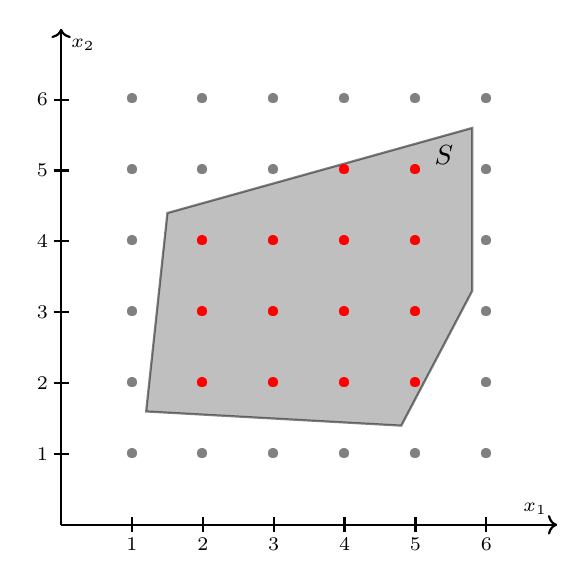
\begin{tikzpicture}[thick, scale=0.9]
    \begin{scope}[thick,font=\scriptsize]
    % Axes:
    % Are simply drawn using line with the `->` option to make them arrows:
    % The main labels of the axes can be places using `node`s:
    \draw [->] (0,0) -- (7,0) node [above left]  {$x_1$};
    \draw [->] (0,0) -- (0,7) node [below right] {$x_2$};
    
    %dotted lines
    %edge points
    %\draw [dashed] (4,0) -- (4,1);
    %\draw [dashed] (0,3) -- (2,3);
    

    % Axes labels:
    % Are drawn using small lines and labeled with `node`s. The placement can be set using options
    \iffalse% Single
    % If you only want a single label per axis side:
    \draw (1,-3pt) -- (1,3pt)   node [above] {$1$};
    \draw (-3pt,1) -- (3pt,1)   node [right] {$1$};
    
    \else% Multiple
    % If you want labels at every unit step:
    \foreach \n in {1,2,...,5,6}{%
        \draw (\n,-3pt) -- (\n,3pt)   node [label=below:$\n$] {};
        \draw (-3pt,\n) -- (3pt,\n)   node [label=left:$\n$] {};
    }
    \fi
    \end{scope}
    % The circle is drawn with `(x,y) circle (radius)`
    % You can draw the outer border and fill the inner area differently.
    % Here I use gray, semitransparent filling to not cover the axes below the circle
   % \path [draw=skiastro,fill=skiastro,semitransparent] (+3,+3) circle (2);1
    
     \node[label=right:] (F) at (4.8,1.4){};
     \node[label=below:] (A) at (1.2,1.6){};
     \node[label=right:] (X) at (5.8,5.6){};
     \node[label=right:] (C) at (5.8,3.3){};
     \draw[thick,fill=gray,semitransparent] (1.5,4.4)  %fills up the figure
     to[bend right=0] (X.center) 
     to[bend left=0] (C.center)
     to[bend left=0] (F.center) 
     to[bend left=0] (A.center) to[bend left=0]  cycle;
    
    % Place the labels of the circle:
    % edge points
 %   \node [below right,darkgray] at (+4,1) {$\pmb{minf_1}$};
%    \node [above left,darkgray] at (2,3) {$\pmb{minf_2}$};
    

    
    %Red points
    %draw edge points
%     \node at (2,3) {\textcolor{red}{\textbullet}};
 %    \node at (4,1) {\textcolor{red}{\textbullet}};    
    
    \node [below,black] at (+5.4,5.5) {$S$};
    
    \node at (1,1) {\textcolor{gray}{\textbullet}};
    \node at (1,2) {\textcolor{gray}{\textbullet}};
    \node at (1,3) {\textcolor{gray}{\textbullet}};
    \node at (1,4) {\textcolor{gray}{\textbullet}};
    \node at (1,5) {\textcolor{gray}{\textbullet}};
    \node at (1,6) {\textcolor{gray}{\textbullet}};
    \node at (2,1) {\textcolor{gray}{\textbullet}};
    \node at (2,2) {\textcolor{red}{\textbullet}};
    \node at (2,3) {\textcolor{red}{\textbullet}};
    \node at (2,4) {\textcolor{red}{\textbullet}};
    \node at (2,5) {\textcolor{gray}{\textbullet}};
    \node at (2,6) {\textcolor{gray}{\textbullet}};
    \node at (3,1) {\textcolor{gray}{\textbullet}};
    \node at (3,2) {\textcolor{red}{\textbullet}};
    \node at (3,3) {\textcolor{red}{\textbullet}};
    \node at (3,4) {\textcolor{red}{\textbullet}};
    \node at (3,5) {\textcolor{gray}{\textbullet}};
    \node at (3,6) {\textcolor{gray}{\textbullet}};
    \node at (4,1) {\textcolor{gray}{\textbullet}};
    \node at (4,2) {\textcolor{red}{\textbullet}};
    \node at (4,3) {\textcolor{red}{\textbullet}};
    \node at (4,4) {\textcolor{red}{\textbullet}};
    \node at (4,5) {\textcolor{red}{\textbullet}};
    \node at (4,6) {\textcolor{gray}{\textbullet}};
    \node at (5,1) {\textcolor{gray}{\textbullet}};
    \node at (5,2) {\textcolor{red}{\textbullet}};
    \node at (5,3) {\textcolor{red}{\textbullet}};
    \node at (5,4) {\textcolor{red}{\textbullet}};
    \node at (5,5) {\textcolor{red}{\textbullet}};
    \node at (5,6) {\textcolor{gray}{\textbullet}};
    \node at (6,1) {\textcolor{gray}{\textbullet}};
    \node at (6,2) {\textcolor{gray}{\textbullet}};
    \node at (6,3) {\textcolor{gray}{\textbullet}};
    \node at (6,4) {\textcolor{gray}{\textbullet}};
    \node at (6,5) {\textcolor{gray}{\textbullet}};
    \node at (6,6) {\textcolor{gray}{\textbullet}};

    \end{tikzpicture}}%picture #1
    \qquad
    %picture #2
    \subfloat[Mixed-Integer Linear Programming problem (MILP), where $x_1 \in \mathbb{R}$ and $x_2 \in \mathbb{Z}$.]{
            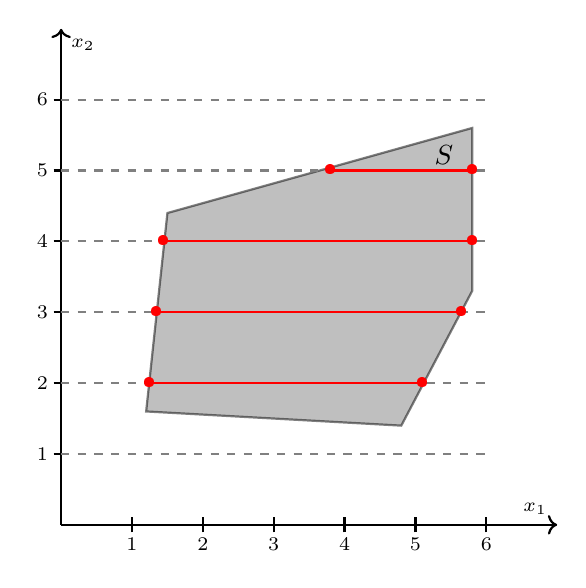
\begin{tikzpicture}[thick, scale=0.9]
    \begin{scope}[thick,font=\scriptsize]
    % Axes:
    % Are simply drawn using line with the `->` option to make them arrows:
    % The main labels of the axes can be places using `node`s:
    \draw [->] (0,0) -- (7,0) node [above left]  {$x_1$};
    \draw [->] (0,0) -- (0,7) node [below right] {$x_2$};
    
    %dotted lines
    %edge points
    %\draw [dashed] (4,0) -- (4,1);
    %\draw [dashed] (0,3) -- (2,3);
    

    % Axes labels:
    % Are drawn using small lines and labeled with `node`s. The placement can be set using options
    \iffalse% Single
    % If you only want a single label per axis side:
    \draw (1,-3pt) -- (1,3pt)   node [above] {$1$};
    \draw (-3pt,1) -- (3pt,1)   node [right] {$1$};
    
    \else% Multiple
    % If you want labels at every unit step:
    \foreach \n in {1,2,...,5,6}{%
        \draw (\n,-3pt) -- (\n,3pt)   node [label=below:$\n$] {};
        \draw (-3pt,\n) -- (3pt,\n)   node [label=left:$\n$] {};
    }
    \fi
    \end{scope}
    % The circle is drawn with `(x,y) circle (radius)`
    % You can draw the outer border and fill the inner area differently.
    % Here I use gray, semitransparent filling to not cover the axes below the circle
   % \path [draw=skiastro,fill=skiastro,semitransparent] (+3,+3) circle (2);1
    
     \node[label=right:] (F) at (4.8,1.4){};
     \node[label=below:] (A) at (1.2,1.6){};
     \node[label=right:] (X) at (5.8,5.6){};
     \node[label=right:] (C) at (5.8,3.3){};
     \draw[thick,fill=gray,semitransparent] (1.5,4.4)  %fills up the figure
     to[bend right=0] (X.center) 
     to[bend left=0] (C.center)
     to[bend left=0] (F.center) 
     to[bend left=0] (A.center) to[bend left=0]  cycle;
    
    % Place the labels of the circle:
    % edge points
 %   \node [below right,darkgray] at (+4,1) {$\pmb{minf_1}$};
%    \node [above left,darkgray] at (2,3) {$\pmb{minf_2}$};
    

    
    %Red points
    %draw edge points
%     \node at (2,3) {\textcolor{red}{\textbullet}};
 %    \node at (4,1) {\textcolor{red}{\textbullet}};    
    
    \node [below,black] at (+5.4,5.5) {$S$};
    
    \draw [gray, dashed] (0,1) -- (6,1);
    \draw [gray, dashed] (0,2) -- (6,2);
    \draw [red, thick] (1.25,2) -- (5.1,2);
    \node at (1.25,2) {\textcolor{red}{\textbullet}};
    \node at (5.1,2) {\textcolor{red}{\textbullet}};
    \draw [gray, dashed] (0,3) -- (6,3);
    \draw [red, thick] (1.4,3) -- (5.6,3);
    \node at (1.35,3) {\textcolor{red}{\textbullet}};
    \node at (5.65,3) {\textcolor{red}{\textbullet}};
    \draw [gray, dashed] (0,4) -- (6,4);
    \draw [red, thick] (1.45,4) -- (5.8,4);
    \node at (1.45,4) {\textcolor{red}{\textbullet}};
    \node at (5.8,4) {\textcolor{red}{\textbullet}};
    \draw [gray, dashed] (0,5) -- (6,5);
    \draw [red, thick] (3.8,5) -- (5.8,5);
    \node at (3.8,5) {\textcolor{red}{\textbullet}};
    \node at (5.8,5) {\textcolor{red}{\textbullet}};
    \draw [gray, dashed] (0,6) -- (6,6);

    \end{tikzpicture}}
    %end of picture #2
    \caption{Illustrations of the Feasible Sets ($S$) of an ILP and a MILP respectively.}%
    \label{fig:Integer Programming figure}%
\end{figure}

%%%%%%%%%%%%%%%%%%%%%%%%%%%%%%%%%%%%%%%%%%%%%%%%%%%%%%%%%%%%%%%%%%%%%%%%%%%%%%%%%%%   SUB SECTION  %%%%%%%%%%%%%%%%%%%%%%%%%%%%%%%%%%%%%%%%%%%%%%%%%%%%%%%%%%%%%%%%%%%

\subsubsection*{Branch and Bound}
The \textit{Branch and Bound (BB)} follows this philosophy of modifying the feasible set until an integer solution is obtained. It begins by obtaining the optimum solution of the relaxed LP. In the case that this initial solution happens to be integer it will immediately terminate since that will mean that the optimum for the original ILP has also been found. If it is not however, the algorithm modifies the LP’s feasible set until its solution satisfies the integrality constraints. \par

\vspace{\baselineskip}
\noindent
Those modifications take place at every iteration, and for the purposes of the BB we refer to them as \textit{branching}. To carry out branching the algorithm divides the solution space into two LP subproblems, by eliminating a part of the LP relaxation’s feasible set that did not contain any feasible integer solutions. For the ILP there is no loss of generality since the union of the subproblems’ feasible sets contains the exact same feasible integer solutions. The two emergent subproblems are then solved separately as regular LPs. Due to the absence of any loss of generality the optimum ILP solution is guaranteed to be in just one of the two new emergent solution spaces of the subproblems. If the solution to either of the two subproblems is worse than any previously known solution, then the corresponding subproblem and its feasible space are disregarded as non-promising. This is known as the \textit{fathoming} step. In essence through such iterations of the algorithm a lower possible bound for the objective value is eventually obtained. \par

\vspace{\baselineskip}
\noindent
By enforcing these two steps iteratively, a binary tree is constructed. Nodes with a non-integer solution have two branching subproblems et cetera. The algorithm is terminated when all nodes will either have an integer solution or a non-integer solution that is worse than the best integer solution of some other node. The node with the most optimum integer solution is the solution to the original ILP \cite{DUMMY:2}.   \par

%%%%%%%%%%%%%%%%%%%%%%%%%%%%%%%%%%%%%%%%%%%%%%%%%%%%%%%%%%%%%%%%%%%%%%%%%%%%%%%%%%%   SUB SECTION  %%%%%%%%%%%%%%%%%%%%%%%%%%%%%%%%%%%%%%%%%%%%%%%%%%%%%%%%%%%%%%%%%%%

\subsubsection*{Cutting Plane}
The \textit{Cutting Plane (CP)} method is also concerned with the transformation of an ILP into a LP that has naturally an integer solution. The process behind this is to gradually cut out part of the relaxed LP's admissible set while leaving the feasible region of the ILP completely unchanged. Hence, eventually upon the implementation of a sufficient number of such \textit{cuts} we will obtain an LP with an integer solution. However, the process of generating the cuts is not a trivial task, and that is the heart of the algorithm. 

\vspace{\baselineskip}
\noindent
The algorithm starts by relaxing the integrality constraints to obtain the LP relaxation of the original ILP. Starting from the optimum solution of the LP relaxation, if it is integer, then the \textit{cutting-plane} algorithm terminates, and this optimum solution is also optimum for the ILP. If it is not, we \textit{tighten} the feasible set of the LP and repeat this process. \par
\vspace{\baselineskip}
\noindent
The \textit{tightening }is done by generating a \textit{cut,} that is a new constraint that restricts unwanted non-integer solutions. This new linear constraint is added to the relaxed LP’s solution space hence modifying $S_{R}$ into a new set $S_{CH}$. This process of modifying $S_{R}$ is repeated until the set converges to one of the ILP’s solution space vertices, at which point the optimum integer solution will have been obtained. Through iteratively performing these steps we create the \textit{convex hull} $S_{CH}$ of the ILP's feasible set $S$.\par

\vspace{\baselineskip}
\noindent
Consequently, starting from the ILP below:

\begin{equation*}
\begin{aligned}
& \underset{x}{\text{minimise}}
& & c^{T}x, \;\;\;\; x \in S \\
\end{aligned}
\end{equation*}

\vspace{\baselineskip}
\noindent
Through generating multiple cuts at each iteration we can instead solve:

\begin{equation*}
\begin{aligned}
& \underset{x}{\text{minimise}}
& & c^{T}x, \;\;\;\; x \in S_{CH} \\
\end{aligned}
\end{equation*}
\[\text{since} \; S \subseteq S_{CH} \subseteq S_{R} \]


\vspace{\baselineskip}
\noindent
The ideal operating scenario for this method would be to generate a relatively small account of highly effective cuts. However, the effectiveness of a cut is a topic with a hard to obtain answer. A universally good cut, would be a cut where the vertex of $S_{CH}$ on which the cut is performed is the furthest from the perimeter of $S_{R}$ since that would automatically mean that the largest possible amount of unwanted feasible space has been cut off. In order generate such good cuts, the simplex algorithm can be utilised. Namely, at each iteration after locating a vertex, we can use the simplex algorithm at that point to determine the best point to pivot to in order to perform the following cut \cite{ieeeeee}.

\vspace{\baselineskip}
\noindent
Overall, a pure cutting plane approach is considered computationally intensive because more often than not, multiple cuts are required. As a direct consequence multiple constraints will be added to the LP relaxation rendering it less computationally tractable. Especially, if we consider that the number of cuts required is not necessarily dependent on the problem’s scale as explained in \cite{DUMMY:3}. In general, there also exist many kinds of cuts such as \textit{Mixed-Integer rounding, }or \textit{Knapsack cover }cuts derived from the logic governing the class packing problems. This adds another variable to the algorithm regarding the choice of cuts. The most prominent are \textit{Gomory mixed-integer }cuts \cite{gomory1958}. Although at the time of their development they were unable to translate their theoretical effectiveness into practice they have recently been revisited and are now considered a go-to method. That is due to the following two reasons. Firstly, due to the emergence of more powerful and robust solvers \cite{cornelio}. Secondly, they have proven to outperform other methods when utilised with a hybrid implementation of the cutting algorithm instead of the pure cutting plane approach. Namely, when utilised a method that combines the \textit{branch-and-bound} with the \textit{cutting-plane} algorithm (i.e. a \textit{branch-and-cut})\cite{BALAS19961} they manage to generate substantially better bounds leading to a decreased computation time compared to the pure versions of those two algorithms \cite{DUMMY:2}.\par

%%%%%%%%%%%%%%%%%%%%%%%%%%%%%%%%%%%%%%%%%%%%%%%%%%%%%%%%%%%%%%%%%%%%%%%%%%%%%%%%%%%    SECTION  %%%%%%%%%%%%%%%%%%%%%%%%%%%%%%%%%%%%%%%%%%%%%%%%%%%%%%%%%%%%%%%%%%%%%%

\subsection*{Duality}
\label{section: Duality}

According to the principle of \textit{duality, }in linear programming every LP can be associated with a corresponding \textit{dual} linear program. The \textit{dual} of a problem is a LP derived from combinations of the constraints of an original LP model, referred to as the \textit{primal.} The solution of the \textit{dual} signifies the best possible bound of the original problem. In matrix form, we can express the \textit{primal} problem as:\par

\vspace{\baselineskip}
\begin{equation*}
\begin{aligned}
& \underset{x}{\text{minimise}}
& & c^{T}x \\
& \text{subject to}
& & Ax \leq b\\
& & & x \geq 0 \\\
\end{aligned}
\end{equation*}

\noindent
with the corresponding \textbf{symmetric} dual problem,\par

\vspace{\baselineskip}
\begin{equation*}
\begin{aligned}
& \underset{x}{\text{minimise}}
& & b^{T}y \\
& \text{subject to}
& & A^{T}y \geq c\\
& & & x \geq 0 \\\
\end{aligned}
\end{equation*}

\noindent
The two problems are completely intertwined with each other. The objective of the primal program is transformed to its mirror-image counterpart in the dual, in a way that if the original is a minimisation problem its dual attempts to maximise the objective function and vice versa. Finding the dual of the dual problem will lead us back to the primal problem. \par
\vspace{\baselineskip}
\noindent
In Linear Programming specifically, the concept of \textit{strong duality }states that the optimum solution to the dual problem is also the optimum for the primal and vice versa. We can leverage this concept when solving LPs where the number of variables is significantly smaller than that of the constraints, since solving the dual will be considerably more computationally efficient and its solution will also be optimum for the original problem. \par

\vspace{\baselineskip}
\noindent
A practical use of the duality concept is that it drives the \textit{post-optimal analysis, }to determine the degree of sensitivity of the optimum solution to any changes in the input parameters. \par

%%%%%%%%%%%%%%%%%%%%%%%%%%%%%%%%%%%%%%%%%%%%%%%%%%%%%%%%%%%%%%%%%%%%%%%%%%%%%%%%%%%   SUB SECTION  %%%%%%%%%%%%%%%%%%%%%%%%%%%%%%%%%%%%%%%%%%%%%%%%%%%%%%%%%%%%%%%%%%%
\subsubsection*{Sensitivity Analysis}

Sensitivity Analysis leverages the relationship between primal-dual problems to calculate the changes in the optimum solution as a result of changes in the input parameters, in an efficient manner. The utility of performing a sensitivity analysis is to gain insights of the relationships between the various components of the problem. For instance, in chapter \ref{chapter: Problem Definition} we will conduct a sensitivity analysis to find out the various the trade-off between the objective function and a variable of the problem. By probing the objective function for various values of that variable we are able to determine the thresholds at which the objective value changes as well as the degree by which it changes. Finally, while performing a sensitivity analysis it is often useful to determine the degree to which a component can remain robust with respect to some changes in another component. For instance, we could establish limits within which changing a certain variable will not cause a change in the optimal solution. Consequently, having done that we will have determined the sensitivity of the optimal solution to changes with respect to that variable.\par

%%%%%%%%%%%%%%%%%%%%%%%%%%%%%%%%%%%%%%%%%%%%%%%%%%%%%%%%%%%%%%%%%%%%%%%%%%%%%%%%%%%   SUB SECTION  %%%%%%%%%%%%%%%%%%%%%%%%%%%%%%%%%%%%%%%%%%%%%%%%%%%%%%%%%%%%%%%%%%%

\subsubsection*{Lagrangian Relaxation}
\addcontentsline{toc}{paragraph}{Lagrangian Relaxation}
The \textit{Lagrangian dual} problem is a bounding technique for solving ILPs that does not disregard the integrality constraints as in previously stated techniques, but instead relaxes some of the main constraints. By forming a combination of the constraints through multiplying them with non-negative Lagrange multipliers, the dual of the original ILP is constructed. The relaxed problem is significantly more computationally tractable, and through solving the dual we can establish a best possible bound for the original ILP.\par

%%%%%%%%%%%%%%%%%%%%%%%%%%%%%%%%%%%%%%%%%%%%%%%%%%%%%%%%%%%%%%%%%%%%%%%%%%%%%%%%%%%    SECTION  %%%%%%%%%%%%%%%%%%%%%%%%%%%%%%%%%%%%%%%%%%%%%%%%%%%%%%%%%%%%%%%%%%%%%%

\section{Multi-Objective Optimisation and Pareto Optimality}
\label{section: Pareto}
Taking a brief diversion from the context of Linear Programming, we look at \textit{Multi-Objective Optimisation} problems where the objective function is comprised of a multitude of objectives. For such problems the \textit{Pareto Optimality} principle proves particularly handy when looking for a \textbf{Pareto optimal} solution. In simple terms To define a Pareto optimal solution we first need to address the concept of a \textbf{dominated solution}: 

\begin{equation}
\begin{aligned}
\label{equation: pareto}
& \underset{x}{\text{minimise}}
& & f(x) \\
& \text{subject to}
& & h_i(x) = 0 \;\;\; i = 1,2, \ldots, m\\
\end{aligned}
\end{equation}
\[where \; x \in \mathbb{Z}^{n} \;, \; f:\mathbb{Z}^{n}\rightarrow \mathbb{Z}^{c}, \; h:\mathbb{Z}^{n}\rightarrow \mathbb{Z}^{m} \]

\vspace{\baselineskip}
\noindent
Given the constrained multi-objective minimisation problem in (\ref{equation: pareto}), that has an objective function $f(x)$ which is a combination of a set of \textit{o} objective functions $f_{1}(x),f_{2}(x),\ldots,f_{o}(x)$ that require simultaneous minimisation, and a feasible space defined by a set of constraints $m$, a feasible solution $d$ is \textbf{dominated} by another feasible solution $s$ if the following two conditions stand:


\begin{equation*}
\begin{aligned}
&(1) \; & &f_{j}(s) \leq f_{j}(d) \; \forall \; j \in [1,\dots,o] \\
&(2) \; & &\exists \; k \in [1,\dots,m] \; | \; f_{k}(s) < f_{k}(d) \\ 
\end{aligned}
\end{equation*}


\vspace{\baselineskip}
\noindent
In simpler terms, these two conditions can be reduced down to: (1) solution $s$ is \textit{as good performing as} $d$ at every objective $o$, and simultaneously, (2) solution $s$ \textbf{strictly} better performing than $d$ at at least one objective \cite{DUMMY:6}. Using the definition of a \textit{dominated} solution, we then define the Pareto optimal solutions as the set of \textbf{undominated} solutions from within the feasible set.

\vspace{\baselineskip}
\noindent
In the context of a practical optimisation problem, finding a feasible point that is concurrently Pareto optimal means that it is only impossible to improve one objective at the expense of another. Hence, it captures the concept of a \textbf{trade-off} between the various objective in the objective function. The reason behind the efficacy of this concept is that more often than not, when presented with a multi-objective optimisation problem it is usually precarious to apply the philosophy of linear programming and trying to optimise multiple objectives in a brute-force way, as it is likely that the optimiser for one of the objective is not going to coincide with that of a different objective. That is because more often than not, especially in problems with numerous objective functions, some objective functions end up being in conflict with each other \cite{grinding}. Hence, we need to address a multi-objective optimisation problem with a slightly different notion of optimality. 

%%%%%%%%%%%%%%%%%%%%%%%%%%%%%%%%%%%%%%%%%%%%%%%%%%%%%%%%%%%%%%%%%%%%%%%%%%%% FIGURE %%%%%%%%%%%%%%%%%%%%%%%%%%%%%%%%%%%%%%%%%%%%%%%%%%%%%%%%%%%%%%%%%%%%%%%%%%%%%%%%

\begin{figure}
    \centering
    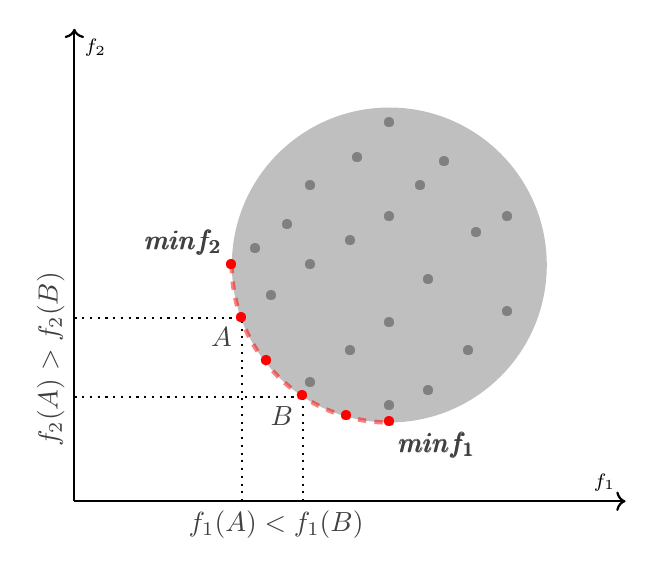
\begin{tikzpicture}
    \begin{scope}[thick,font=\scriptsize]
    % Axes:
    % Are simply drawn using line with the `->` option to make them arrows:
    % The main labels of the axes can be places using `node`s:
    \draw [->] (0,0) -- (7,0) node [above left]  {$f_1$};
    \draw [->] (0,0) -- (0,6) node [below right] {$f_2$};
    
    %dotted lines
    %edge points
    %\draw [dashed] (4,0) -- (4,1);
    %\draw [dashed] (0,3) -- (2,3);
    
    %A
    \draw [dotted] (2.125,0) -- (2.125,2.328);
    \draw [dotted] (0,2.328) -- (2.125,2.328);
    
    %B
    \draw [dotted] (2.9,0) -- (2.9,1.325);
    \draw [dotted] (0,1.325) -- (2.9,1.325);

    % Axes labels:
    % Are drawn using small lines and labeled with `node`s. The placement can be set using options
    \iffalse% Single
    % If you only want a single label per axis side:
    \draw (1,-3pt) -- (1,3pt)   node [above] {$1$};
    \draw (-3pt,1) -- (3pt,1)   node [right] {$1$};
    
    \else% Multiple
    % If you want labels at every unit step:

    \fi
    \end{scope}
    % The circle is drawn with `(x,y) circle (radius)`
    % You can draw the outer border and fill the inner area differently.
    % Here I use gray, semitransparent filling to not cover the axes below the circle
    \path [draw=none,fill=gray,semitransparent] (+4,+3) circle (2);
    \path [draw=red, ultra thick,fill=none,semitransparent, dashed] (+2,+3) arc[start angle=180, end angle=270, radius=2];
    
    % Place the labels of the circle:
    % edge points
    \node [below right,darkgray] at (+4,1) {$\pmb{minf_1}$};
    \node [above left,darkgray] at (2,3) {$\pmb{minf_2}$};
    
    %A,B
    \node [below left,darkgray] at (2.9,1.325) {$B$};
    \node [below left,darkgray] at (2.125,2.328) {$A$};
    
    \node [below,darkgray] at (2.5625,0) {$f_1(A)<f_1(B)$};
    \node [above ,darkgray,rotate=90] at (0,1.801) {$f_2(A)>f_2(B)$};
    
    %Red points
    %draw edge points
     \node at (2,3) {\textcolor{red}{\textbullet}};
     \node at (4,1) {\textcolor{red}{\textbullet}};    
     
    %draw MIDWAY points
     %\node at (2.0425,2.6) {\textcolor{red}{\textbullet}};
     \node at (2.125,2.318) {\textcolor{red}{\textbullet}}; %A
     %\node at (2.25,2.032) {\textcolor{red}{\textbullet}};
     \node at (2.435,1.777) {\textcolor{red}{\textbullet}};    
     %\node at (2.75,1.439) {\textcolor{red}{\textbullet}};    
     \node at (2.9,1.325) {\textcolor{red}{\textbullet}}; %B
     \node at (3.45,1.075) {\textcolor{red}{\textbullet}};    
     

     \node at (2.3,3.2) {\textcolor{gray}{\textbullet}};
     \node at (2.5,2.6) {\textcolor{gray}{\textbullet}};
     \node at (3,1.5) {\textcolor{gray}{\textbullet}};
     
     \node at (2.7,3.5) {\textcolor{gray}{\textbullet}};
     \node at (3,3) {\textcolor{gray}{\textbullet}};
     \node at (3.5,1.9064) {\textcolor{gray}{\textbullet}};
     \node at (4,1.2) {\textcolor{gray}{\textbullet}};

     \node at (3,4) {\textcolor{gray}{\textbullet}};
     \node at (3.5,3.3) {\textcolor{gray}{\textbullet}};
     \node at (4,2.264) {\textcolor{gray}{\textbullet}};
     \node at (4.5,1.4) {\textcolor{gray}{\textbullet}};

     \node at (3.6,4.35) {\textcolor{gray}{\textbullet}};
     \node at (4,3.6) {\textcolor{gray}{\textbullet}};
     \node at (4.5,2.8) {\textcolor{gray}{\textbullet}};
     \node at (5,1.9) {\textcolor{gray}{\textbullet}};
     
     \node at (4,4.8) {\textcolor{gray}{\textbullet}};
     \node at (4.4,4) {\textcolor{gray}{\textbullet}};
     \node at (4.7,4.3) {\textcolor{gray}{\textbullet}};
     \node at (5.1,3.4) {\textcolor{gray}{\textbullet}};
     \node at (5.5,3.6) {\textcolor{gray}{\textbullet}};
     \node at (5.5,2.4) {\textcolor{gray}{\textbullet}};

    \end{tikzpicture}
    \caption{The image of the feasible set of a Bi-Objective Optimisation problem showcasing the Pareto Front.}
    \label{fig:Pareto figure}
\end{figure}

\vspace{\baselineskip}
\noindent
Suppose, we are given a constrained multi-objective optimisation problem similar to (\ref{equation: pareto}), where $o=2$, (i.e. our problem has only two objectives). Plotting the image of the feasible set of this problem on the plane ($f_1,f_2$), as seen in Figure \ref{fig:Pareto figure} \cite{Taheri2014ParetoFF} can help us locate the \textbf{minimum} for each objective with respect to all feasible solutions. However, upon trying to simultaneously minimise $f_1,f_2$ one can see from the figure that $minf_1$ is not particularly optimal for $f_2$ and vice versa. If one chooses to minimise $f_1$ by choosing point $minf_1$, they do so at the expense of $f_2$. Hence, according to the Pareto principle we characterise the set of points in between $minf_1,minf_2$ as \textit{Pareto optimal}, representing the points for which one cannot improve any of the objectives without sacrificing one of the others. These set of points is represented by the red-coloured boundary of the image of the feasible set, and are often seen as \textbf{efficient frontier} in literature.

\vspace{\baselineskip}
\noindent
All in all, this new notion of optimality defined through the Pareto principle refers to the difference in the approach followed for the solution of a standard linear program compared to a multi-objective problem untangled with the Pareto concept. Instead of attempting to minimise all objectives at once, which would most likely prove ineffective, we instead solve the problem for each objective separately to get an overall depiction of the optimal feasible solutions through a figure like that in Figure \ref{fig:Pareto figure} then leaving it up to the optimiser to decide the best compromises to be made. This philosophy can be summarised in the following steps \cite{DUMMY:6}:

\begin{algorithm}[H]
\SetAlgoLined
\KwResult{End points of the efficient frontier ($minf_1,minf_2$)}
 initialization: i=1\;
 \For{i<o}{
  i+1\;
  $minimise \; f_i$\;
  find the value $s_j$ for objective $j\neq i$\;
  ($minf_i,s_j$) is a point on the efficient frontier\;
  \eIf{there do not exist dominant points $s$ with respect to objective j}{
   $minimise \; f_j$ where $j\neq i$ \; to find ($minf_j,s_i$)\;
   }{
   points ($f_i(s), f_j(s)$) belonging on the efficient frontier\;
  }
 }
 \caption{How to obtain the \textbf{efficient frontier}}
 \label{alg: Pareto}
\end{algorithm}

%%%%%%%%%%%%%%%%%%%%%%%%%%%%%%%%%%%%%%%%%%%%%%%%%%%%%%%%%%%%%%%%%%%%%%%%%%%%%%%%%%%    SECTION  %%%%%%%%%%%%%%%%%%%%%%%%%%%%%%%%%%%%%%%%%%%%%%%%%%%%%%%%%%%%%%%%%%%%%%
\section{Optimisation under Uncertainty}
\label{section:background uncertainty}
\subsection{Robust Optimisation}
In general there are mostly two approaches to model uncertainty within the context of optimisation, Stochastic Optimisation and Robust Optimisation. For the purposes of this dissertation we focus on the \textit{robustness} of our models which we define as the quality of a method to remain feasible even after the application of an \textbf{uncertain set} $U$ on it. Utilising the formulation (\ref{equation: LP compact form}) we can write the robust version of an LP as \cite{Bertsimas2011TheoryAA}:

\vspace{\baselineskip}
\begin{equation}
\label{equation: robust compact form}
\begin{aligned}
& \underset{x}{\text{minimise}}
& & c^{T}x \\
& \text{subject to}
& & Ax \leq b & \forall a_1 \in U_1,\ldots, a_m \in U_m\\
& & & x \geq 0 \\\
\end{aligned}
\end{equation}
\[where \; b \geq 0 \; and \; A \in \mathbb{R}^{m \times n}, \; b \in \mathbb{R}^{m}, \; c \in \mathbb{R}^{n} \; \text{and }  U_i \in \mathbb{R}^{n}\]

%%%%%%%%%%%%%%%%%What is the price of robustness of an initial solution. 

\vspace{\baselineskip}
\noindent
More specifically, in terms of comparing the \textit{robustness} of two solutions to a problem we argue the following. Assume one has an optimisation problem, for instance a \textit{MILP}, which has a certain objective function, and one can obtain a certain number of \textit{solutions} for it through a certain set of \textit{methods}. Upon, applying the uncertain set $U$ on the different solutions, we characterise as \textbf{more robust} the method that after uncertainty provides the solutions with the best objective value.

%%%%%%%%%%%%%%%%%%%%%%%%%%%%%%%%%%%%%%%%%%%%%%%%%%%%%%%%%%%%%%%%%%%%%%%%%%%%%%%%%%%   SUB SECTION  %%%%%%%%%%%%%%%%%%%%%%%%%%%%%%%%%%%%%%%%%%%%%%%%%%%%%%%%%%%%%%%%%%%

\subsubsection*{Robust Optimisation under Uncertainty}
One of the fundamental elements of Robust Optimisation are uncertainty sets. An interval-based uncertain set $U$, is defined by a \textit{lower} and an \textit{upper} bound, such that an instance of the random variable $s$ is enclosed in the following \cite{Bertsimas2011TheoryAA}, \cite{robustuncertainty}:

\vspace{\baselineskip}
\begin{equation}
\begin{aligned}
& U \; = \; \prod_{i\in n} \{s_i \in \mathbb{R}^{n} \; | \; \underline{s_i} \leq s_i \leq  \overline{s_i}\} \text{    for Box Uncertainty Set} \\
\end{aligned}
\end{equation}

\vspace{\baselineskip}
\noindent
Hence, one can now generate instances $I$ of a problem that have this uncertainty set $U$ applied to it, from the following \textbf{spectrum of Instances}: $I_{lower}$ (every $s$ is $\underline{s}$), $I_{middle}$ (every $s$ is $\frac{\underline{s}+\overline{s}}{2}$), and $I_{upper}$ (every $s$ is $\overline{s}$). If we assume that $s$ is enclosed in a ball of radius $\Omega$ centered at the origin \cite{robustoptimisation}, we can have the following \cite{christodoulos},\cite{GORISSEN2015124}:

\vspace{\baselineskip}
\begin{equation}
\begin{aligned}
& U \; = \; \prod_{i\in n} \{s \in \mathbb{R}^{n} \; | \; \sum _{i=1}^{n}s_{i}^2  \leq  \Omega^2 \} \text{    for Ellipsoidal Uncertainty Set} \\
\end{aligned}
\end{equation}

\vspace{\baselineskip}
\noindent
However, in order to use the concept of \textit{uncertainty sets} to simulate the concept of uncertainty in real-life one should select values of $s$ \textbf{at random} from within $[\underline{s},\overline{s}]$, as this will be a fairer representation of the chaotic randomness that tends to occur in reality.

\vspace{\baselineskip}
\noindent
Generally speaking the generation of uncertainty set is not a trivial matter. D. Bertsimas and D. Brown develop a theory in \cite{concstructuncertaity} revolved around the generation of uncertainty sets that replicate explicit uncertainty sets as far as their structure and behavior. 


%%%%%%%%%%%%%%%%%%%%%%%%%%%%%%%%%%%%%%%%%%%%%%%%%%%%%%%%%%%%%%%%%%%%%%%%%%%%%%%%%%%    SECTION  %%%%%%%%%%%%%%%%%%%%%%%%%%%%%%%%%%%%%%%%%%%%%%%%%%%%%%%%%%%%%%%%%%%%%%

\section{Vehicle Routing Problems}
\label{section: vrp}
Our problem can be interpreted as a \textit{Vehicle Routing Problem (VRP)}. We do not explicitly focus on the study of the routing of the problem, but instead focus on the scheduling aspect and only utilise some concepts derived from the \textit{VRP} discipline in our project. Nevertheless, we propose the application of the routing aspect of the \textit{VRP} philosophy on our problem as one of the future directions that need to be explored in the context of our problem. Hence, we include below a brief study, that aims to give the reader a high-level overview of this class of problems.

\vspace{\baselineskip}
\noindent
\textit{Vehicle Routing Problems (VRP)} have been studied intensely over the years, and well known survey papers such as \cite{doi:surveyVRP} can give an interested reader further information on the problem. Moreover, the following paper \cite{LAPORTE1992345} outlines the most frequently used algorithms towards efficient solving of problems of this context. Such algorithms are used for the purposes of a formulation seen in Section \ref{section: Pre-emptive} of Chapter \ref{chapter: 2-Evaluating Royal Mail Historical Data}, where the vehicle routing aspect of our problem is studied. Moreover, given that the application of the vehicle routing concepts on our problem is presented as one of the directions for future research, we believe that a careful study of efficient approximation algorithms such as those studied in \cite{approx} would be purposeful. 



%%%%%%%%%%%%%%%%%%%%%%%%%%%%%%%%%%%%%%%%%%%%%%%%%%%%%%%%%%%%%%%%%%%%%%%%%%%%%%%%%%%    SECTION  %%%%%%%%%%%%%%%%%%%%%%%%%%%%%%%%%%%%%%%%%%%%%%%%%%%%%%%%%%%%%%%%%%%%%%

\section{Multiprocessor Scheduling Problems}

Scheduling problems are a common class of decision-making problems that deal with the search for the most efficient method of allocating resources to tasks. This search for efficiency is explored by attempting to optimise a single or multiple objectives related to the problem which eventually leads us to the most suitable schedule for each problem. In real world professional environments, suitable task schedules are critical to ensure a good balance of the load amongst the parallel machines \cite{DUMMY:2}.\par
\vspace{\baselineskip}
\noindent
There are numerous kinds of scheduling problems. This dissertation focuses on the class of deterministic problems that are supplied as input a collection of tasks requiring processing on an environment comprised of a bank of identical parallel machines. In \textit{deterministic} problems, the input data is made available prior to the optimisation process and the aim is to come up with the most efficient sequence of these jobs, subject to a set of constraints, that optimises one or more performance criteria. This task can be broken down to, deciding which tasks have to be allocated to each machine as well as how to sequence the jobs dispatched to each machine. Machines can process at most one job on any given moment in time, and will see a job to its completion once its execution has begun. \par

%%%%%%%%%%%%%%%%%%%%%%%%%%%%%%%%%%%%%%%%%%%%%%%%%%%%%%%%%%%%%%%%%%%%%%%%%%%%%%%%%%%   SUB SECTION  %%%%%%%%%%%%%%%%%%%%%%%%%%%%%%%%%%%%%%%%%%%%%%%%%%%%%%%%%%%%%%%%%%%

\subsection*{Makespan Scheduling}
\label{section:Makespan Scheduling}
In \textit{makespan} scheduling problems, the objective function to be minimised is the \textit{makespan (\( C_{\max }\)})\textit{. }The \textit{makespan }defined as  \( max \left( C_{1},C_{2},...,C_{n} \right)   \) is equivalent to the point in time that signifies the \textbf{termination} of the\textbf{ last job} to be \textbf{completed}. Our goal is to sequence the jobs in question, in an efficient manner that enables the last job to finish processing as early as possible, while respecting the specified set of constraints. In essence, this type of problems resemble the generalised bin-packing problems in the context of scheduling \cite{Coffman1978AnAO}. The minimisation of the makespan is one of the most utilised optimality criteria \cite{schedalgos} because striving to minimise the overall makespan of a schedule more often than not, results in a schedule that achieves a well-balanced sequence of jobs \cite{DUMMY:2}. \par
\vspace{\baselineskip}
\noindent
\textbf{Set of Input Data}

\vspace{\baselineskip}
{\addtolength{\leftskip}{5mm}
\noindent
\( Set~M= \{ 1,2,...,m \}  \)  specifies an environment of \textit{m} parallel and identical machines. 

\vspace{\baselineskip}
\noindent
\( Set~J= \{ 1,2, \ldots ,n \}  \) represents the number of jobs that await to be sequenced on each machine.\par
 
 \vspace{\baselineskip}
 \noindent
The n-dimensional vector \textbf{p} contains the processing time \( p_{j} \) of job \( j .\)\par

}

\vspace{\baselineskip}
\noindent
\textbf{Parallel Machine model}

\vspace{\baselineskip}
\begin{equation}
\label{equation: makespan background}
\begin{aligned}
& \underset{x_{ij}}{\text{minimise}}
& & C_{\max } \\
& \text{subject to}
& &  C_{\max } \geq \sum _{j=1}^{n}x_{ij} \cdot p_{j}~~ \;\;\; &\text{for } i \in M\\
& & & \sum _{i=1}^{m}x_{ij} = 1\;\;\; &\text{for } j \in J\\
& & & x_{ij} \in  \{ 0,1 \} \;\;\; &\text{for } i \in M, \; j \in J\\
\end{aligned}
\end{equation}

\vspace{\baselineskip}
\noindent
The first constraint reflects the definition of the \textit{makespan}, and makes sure that it takes the value of the completion time of the last job to be completed. The second constraint enforces that each job is executed once and only once throughout the spectrum of all the machines. Finally, the third constraint is the integrality constraint of such a \textit{MILP} problem.   

\vspace{\baselineskip}
\noindent
As we can see, Figure \ref{fig:intro gantt chart} contains an example of two schedules\cite{DUMMY:2}. The example is meant to illustrate the effect of applying a Makespan Scheduling formulation on the non-optimised schedule seen in \ref{fig:intro gantt chart}(a). In this case the set of input data is the following:

\begin{itemize}
    \item \\
    \item We have nine jobs each with their own processing time $p_j$.\\
\end{itemize}

\vspace{\baselineskip}
{\addtolength{\leftskip}{5mm}
\noindent
We have four parallel and identical machines.\par

\vspace{\baselineskip}
\noindent
We have nine jobs each with their own processing time $p_j$.\par
 
}

\vspace{\baselineskip}
\noindent
We can see that by applying this set of input data to formulation \ref{equation: makespan background} we get a reduction in the makespan of the schedule in \ref{fig:intro gantt chart}(a) from 15 hours down to 12 hours in in \ref{fig:intro gantt chart}(b). Moreover, as expected the workload of all machines is considerably more balanced since they are all of a duration equal to 12 hours. Indeed, it is true however, that those duties that we originally below the 12 hour mark have seen their duration increased (up to the 12 hour mark).

%%%%%%%%%%%%%%%%%%%%%%%%%%%%%%%%%%%%%%%%%%%%%%%%%%%%%%%%%%%%%%%%%%%%%% Figure %%%%%%%%%%%%%%%%%%%%%%%%%%%%%%%%%%%%%%%%%%%%%%%

%Two images in one, illustrating atomic block
\begin{figure}%
    \centering
    \subfloat[Un-optimised that our model receives as input for rescheduling.]{
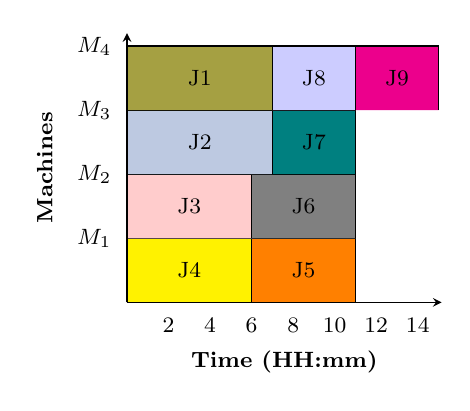
\begin{tikzpicture}
\begin{axis}[
  font=\footnotesize,
  ytick style={draw=none},
  xtick style={draw=none},
  %unit vector ratio*=1 1 1,%1 0.6 1,
  axis lines = middle,
  enlarge x limits = {value=.01,upper},
  enlarge y limits = {value=.05,upper},
  ylabel={\textbf{Machines}},
  xlabel={\textbf{Time (HH:mm)}},
  ylabel near ticks,
  xlabel near ticks,
  const plot,
  stack plots=false,
  area style,
  width=0.46\textwidth,
  height=5cm, %control the height of chart
  %width=\linewidth,height=\textheight,
  ytick={1,...,60},
  yticklabels={},  
  xtick={0,2,...,24},,
  extra y ticks={1,2,3,4},
  extra y tick style={yticklabel={$M_{\pgfmathprintnumber{\tick}}$}}
  ] 
\addplot[fill=yellow] coordinates {(0,0) (0,1) (6,1) (6,0) } node at (current path bounding box.center) {J4};
\addplot[fill=orange] coordinates {(6,0) (6,1) (11,1) (11,0) } node at (current path bounding box.center) {J5};
\addplot[fill=red!20] coordinates {(0,1) (0,2) (6,2) (6,1) } node at (current path bounding box.center) {J3};
\addplot[fill=gray] coordinates {(6,1) (6,2) (11,2) (11,1) } node at (current path bounding box.center) {J6};
\addplot[fill=light blue] coordinates {(0,2) (0,3) (7,3) (7,2) } node at (current path bounding box.center) {J2};
\addplot[fill=teal] coordinates {(7,2) (7,3) (11,3) (11,2) } node at (current path bounding box.center) {J7};
\addplot[fill=yellow!60!black] coordinates {(0,3) (0,4) (7,4) (7,3) } node at (current path bounding box.center) {J1};
\addplot[fill=blue!20] coordinates {(7,3) (7,4) (11,4) (11,3) } node at (current path bounding box.center) {J8};
\addplot[fill=magenta] coordinates {(11,3) (11,4) (15,4) (15,3) } node at (current path bounding box.center) {J9};
\end{axis}
\end{tikzpicture}}%picture #1
    \qquad
    %picture #2
    \subfloat[Rescheduled and Makespan optimised Schedule.]{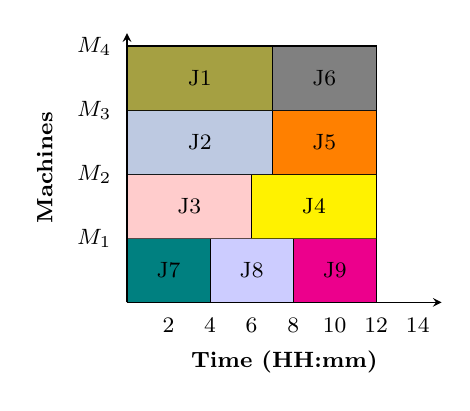
\begin{tikzpicture}
\begin{axis}[
  font=\footnotesize,
  ytick style={draw=none},
  xtick style={draw=none},
  %unit vector ratio*=1 1 1,%1 0.6 1,
  axis lines = middle,
  enlarge x limits = {value=.01,upper},
  enlarge y limits = {value=.05,upper},
  ylabel={\textbf{Machines}},
  xlabel={\textbf{Time (HH:mm)}},
  ylabel near ticks,
  xlabel near ticks,
  const plot,
  stack plots=false,
  area style,
  width=0.46\textwidth,
  height=5cm, %control the height of chart
  %width=\linewidth,height=\textheight,
  ytick={1,...,60},
  yticklabels={},  
  xtick={0,2,...,24},
  extra y ticks={1,2,3,4},
  extra y tick style={yticklabel={$M_{\pgfmathprintnumber{\tick}}$}}
  ] 
\addplot[fill=teal] coordinates {(0,0) (0,1) (4,1) (4,0) } node at (current path bounding box.center) {J7};
\addplot[fill=blue!20] coordinates {(4,0) (4,1) (8,1) (8,0) } node at (current path bounding box.center) {J8};
\addplot[fill=magenta] coordinates {(8,0) (8,1) (12,1) (12,0) } node at (current path bounding box.center) {J9};
\addplot[fill=red!20] coordinates {(0,1) (0,2) (6,2) (6,1) } node at (current path bounding box.center) {J3};
\addplot[fill=yellow] coordinates {(6,1) (6,2) (12,2) (12,1) } node at (current path bounding box.center) {J4};
\addplot[fill=light blue] coordinates {(0,2) (0,3) (7,3) (7,2) } node at (current path bounding box.center) {J2};
\addplot[fill=orange] coordinates {(7,2) (7,3) (12,3) (12,2) } node at (current path bounding box.center) {J5};
\addplot[fill=yellow!60!black] coordinates {(0,3) (0,4) (7,4) (7,3) } node at (current path bounding box.center) {J1};
\addplot[fill=gray] coordinates {(7,3) (7,4) (12,4) (12,3) } node at (current path bounding box.center) {J6};
\addplot[fill=none,opacity=0.0] coordinates {(12,3) (12,4) (15,4) (15,3) } node at (current path bounding box.center) {};
\end{axis}
\end{tikzpicture}}
    %end of picture #2
    \caption{Illustrations showing the process of \textbf{Rescheduling} implemented throughout this dissertation.}%
    \label{fig:intro gantt chart}%
\end{figure}


\subsubsection{Longest Processing Time}

In order to achieve an effective sequencing of the jobs, heuristics such as the \textit{Longest Processing Time first (LPT)}  rule have been developed. According to this algorithm, the \textit{m} first jobs with the longest processing times  \( p_{j} \)  are assigned at the start to the \textit{m} available machines. The first machine, out of the batch of those \textit{m} machines to finish its execution is subsequently assigned the job with the longest processing time amongst those remaining, and so forth. It turns out by definition, that the job with the shortest processing time is the last one to begin its processing. \par

%%%%%%%%%%%%%%%%%%%%%%%%%%%%%%%%%%%%%%%%%%%%%%%%%%%%%%%%%%%%%%%%%%%%%%%%%%%%%%%%%%%   SUB SECTION  %%%%%%%%%%%%%%%%%%%%%%%%%%%%%%%%%%%%%%%%%%%%%%%%%%%%%%%%%%%%%%%%%%%
\subsection*{Time-Indexed Models}

In \textit{time-indexed} formulations, we choose to add the dimension of \textit{time} to our model. We can express the same problem with a \textit{discrete time} formulation, by splitting continuous time \( t \) into \( T \) discrete intervals. Consequently we have that, $ t \in T = \{0,1,\ldots,T-1\} $. We then use binary variable \( x_{ijt} \) which equals to \( 1 \) if job \( j \) starts at time \( t \) on machine \( i \) and equal to \( 0 \) the rest of the time \cite{DUMMY:2}.  \par


\vspace{\baselineskip}
\begin{equation}
\begin{aligned}
& \underset{x_{ijt}}{\text{minimise}}
& & \sum _{i=1}^{m}\sum _{j=1}^{n}\sum _{t=0}^{C_{\max }-1}x_{ijt} \cdot (t+p_{j}) \\
& \text{subject to}
& & \sum _{i=1}^{m}\sum _{t=0}^{C_{\max }-1} x_{ijt} = 1 \;\;\; &\text{for } j \in J\\
& & & \sum _{j=1}^{n}\sum _{s=max(t-p_{j},0)}^{t-1}x_{ijt} = 1 \;\;\; &\text{for } t \in T, \; i \in M\\
& & & \sum _{i=1}^{m}\sum _{j=1}^{n}\sum _{s=max(t-p_{j},0)}^{t-1}x_{ijt} \leq m \;\;\; &\text{for } t \in T\\
& & & x_{ijt} \in  \{ 0,1 \} \;\;\; &\text{for } i \in M, \; j \in J, \; t \in T\\
\end{aligned}
\end{equation}

\vspace{\baselineskip}
\noindent
With the first constraint we make sure that each job is executed once and only once throughout all the machines. The second constraint enforces the definition of the environment of machines, namely that each machine does not process more than one job at any given moment in time. The third constraint is in place to prevent the possibility of more jobs being executed at some point in time, than there are machines available in the environment. Finally, the last constraint reflects the integrality constraint of such a \textit{MILP} problem.   

\vspace{\baselineskip}
\noindent
Comparing this time-indexed formulation with that in (2.5), it is visible that (2.6) will result in substantially more variables being used, ($m$$\cdot$$n$$\cdot$$C_{max}$)-many $x_{ijt}$ variables to be exact. Come solution time, this will be a factor that slows down the process of obtaining a solution to (2.6).
\vspace{\baselineskip}

%%%%%%%%%%%%%%%%%%%%%%%%%%%%%%%%%%%%%%%%%%%%%%%%%%%%%%%%%%%%%%%%%%%%%%%%%%%%%%%%%%%   SUB SECTION  %%%%%%%%%%%%%%%%%%%%%%%%%%%%%%%%%%%%%%%%%%%%%%%%%%%%%%%%%%%%%%%%%%%

\subsection*{Pareto Optimal Schedule}
Returning to the context of the scheduling problem, we can characterise a schedule Pareto optimal provided we cannot minimise one of its objectives without
incurring an expense for another objective, as expected from the definition of a Pareto optimal solution in Section \ref{section: Pareto}.

\todo{write more from scheduling book on pareto}


\section{System Specifications}
All computations are processed with a 6-core Intel Core i7 CPU running at 2.60GHz with a 16GB RAM memory on a macOS Catalina (version 10.15.4) machine. The models were implemented using C++11 that was compiled with the GNU Compiler Collection (GCC). The solutions were obtained through using the commercial solver CPLEX 12.9. Unless it is specifically stated, all solutions obtained are the optimal ones for the given objective function, set of constraints and decision variables.   


\vspace{\baselineskip}

\vspace{\baselineskip}

\vspace{\baselineskip}

\vspace{\baselineskip}

\chapter{Data Exploration and Scheduling Problem Building Blocks}
\label{chapter: Problem Definition}

%%%%%%%%%%%%%%%%%%%%%%%%%%%%%%%%%%%%%%%%%%%%%%%%%%%%%%%%%%%%%%%%%%%%%%%%%%%%%%% SECTION %%%%%%%%%%%%%%%%%%%%%%%%%%%%%%%%%%%%%%%%%%%%%%%%%%%%%%%%%%%%%%%%%%%%%%%%%%%%%%

In this chapter we re-introduce the problem assigned to us by Royal Mail in a greater level of detail. Sections \ref{section: problem outline}-\ref{section: Input Parameters} walk the reader through a more detailed description of the problem to introduce them to the main elements that constitute the problem as well as give them an idea of Royal Mail's current practices through a series of examples. They also outline the motivation behind solving this problem, and provide arguments justifying why this is a problem worthwhile solving, with great potential for efficiency gains despite the complexity involved in obtaining a solution. 

\vspace{\baselineskip}
\noindent
Following the description of the problem, Section \ref{section: Data Exploration} continues by outlining the structure of the historical data supplied by Royal Mail, and the steps taken to bring the dataset in the form that was utilised in the modelling portion of the project. The \textbf{finalised} form of the dataset described at the end of the Data Cleaning section \ref{section: Data Cleaning} constitutes the foundation upon which this dissertation will derive feasible, and efficient schedules. The chapter concludes with Sections \ref{section: Redefined Dataset}-\ref{fig: Wave-instances.} describing the processes behind the generation of two unique instances of the problem that will be utilised to conduct more targeted experiments in Chapter \ref{chapter: 2-Evaluating Royal Mail Historical Data}. 

\vspace{\baselineskip}
\noindent
All in all, this chapter gives a more detailed overview of the problem, as well as a detailed description of the dataset provided by our Industrial Liaison, and the steps taken to prepare it for use in our experiments. 

%%%%%%%%%%%%%%%%%%%%%%%%%%%%%%%%%%%%%%%%%%%%%%%%%%%%%%%%%%%%%%%%%%%%%% Section %%%%%%%%%%%%%%%%%%%%%%%%%%%%%%%%%%%%%%%%%%%%%%%

\section{General Context}
\label{section: problem outline}
Each of Royal Mail's \textbf{Mail Centres (MC)} upon receiving the mail collected from each \textbf{Delivery Office (DO)} will sort it and then decide which portions of it need to be redistributed to DOs belonging to the same MC the following day. Our goal is to structure the delivery itinerary for each MC, for the portion of the post that will remain within the circulation of that MC. 


\vspace{\baselineskip}
\noindent
The day before a piece of mail is delivered, the MC responsible for it will have a set of round-trips that need to be completed. At its disposal, each MC has a crew of \textbf{HGV drivers}, that will complete those trips. Our objective, is to schedule those trips in a more efficient manner than Royal Mail's current scheduling practices, that minimises the time that drivers spend performing \textbf{non-essential} activities that could be performed by lower-grade employees. The process of creating those schedules can be resolved into two sub-components. \textbf{Firstly}, decide which trips are completed by each driver. \textbf{Secondly}, decide how to sequence the trips assigned to each driver. In allocating trips to a driver we need to respect some restrictions imposed by certain parameters on whether a trip can be allocated to each specific driver, on a particular instant in time. These restrictions are driven by the EU regulations\footnote{Further explained in Appendix \ref{section: EU rules}} around HGV drivers, in particular the \textit{driving} and \textit{working} time directives. However, for the purposes of this dissertation we neglect those, hence our focus is solely concerned with the task of finding the \textbf{room} available \textbf{for optimisation}. Following that, it should be straightforward to make the modelling more realistic by introducing those important constraints that ensure the utmost legality of the schedules and it is one of the direction considered for future work\footnote{Further explained in Section \ref{section: Addition of the Meal Relief Constraint} of Chapter \ref{chapter: Future Directions}} on the problem. 

\vspace{\baselineskip}
\noindent
As mentioned in the Introduction chapter of the report, we only focus on the \textbf{scheduling} aspect of the problem, and consider the routes to be fixed, hence we do not focus on the \textit{Vehicle Routing} point of view.


%%%%%%%%%%%%%%%%%%%%%%%%%%%%%%%%%%%%%%%%%%%%%%%%%%%%%%%%%%%%%%%%%%%%%% Figure %%%%%%%%%%%%%%%%%%%%%%%%%%%%%%%%%%%%%%%%%%%%%%%

\begin{figure}
    \centering
	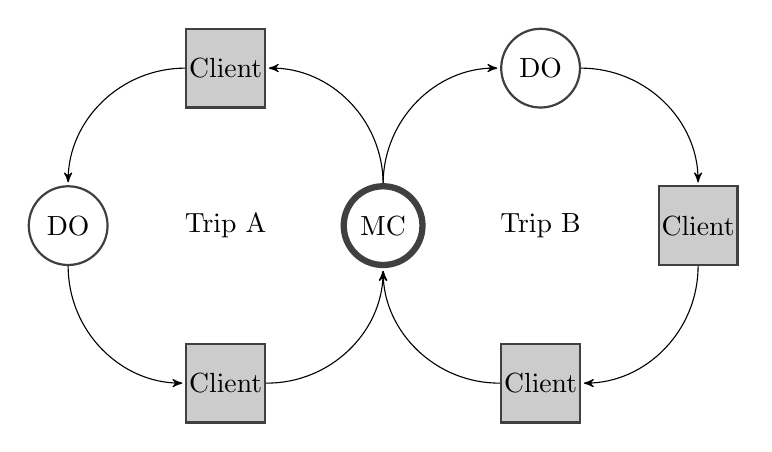
\begin{tikzpicture}[node distance=2cm,>=stealth',bend angle=45,auto,rotate=90,transform shape]%picture #1

      \tikzstyle{place}=[circle,thick,draw=black!75,fill=white!20,minimum size=10mm]
      \tikzstyle{red place}=[place,draw=red!75,fill=red!20]
      \tikzstyle{transition}=[rectangle,thick,draw=black!75,
      			  fill=black!20,minimum size=10mm]
    
      \tikzstyle{every label}=[black]
    
      \begin{scope}
        
        
        %All but clients
        \node [place,label={[rotate=-90]center:DO}] (w1)                                    {};
        \node [place, draw=white,label={[rotate=-90]center:Trip A}] (c1) [below of=w1]                      {};
        \node [place, line width=0.8mm,label={[rotate=-90]center:MC}] (s)  [below of=c1] {};
        \node [place, draw=white,label={[rotate=-90]center:Trip B}] (c2) [below of=s]                       {};
        \node [place,label={[rotate=-90]center:DO}] (w2) [right of=c2]                      {}
            edge [pre,bend right]                (s);
    
        %boxes w/ Clients
        \node [transition,label={[rotate=-90]center:Client}] (e1) [left of=c1] {}
          edge [pre,bend left]                  (w1)
          edge [post,bend right]                (s);
    
        \node [transition,label={[rotate=-90]center:Client}] (e2) [left of=c2] {}
          edge [post,bend left]                 (s);
    
        \node [transition,label={[rotate=-90]center:Client}] (l1) [right of=c1] {}
          edge [pre,bend left]                  (s)
          edge [post,bend right] node[swap] {} (w1);
    
        \node [transition,label={[rotate=-90]center:Client}] (l2) [below of=c2] {}
          edge [pre,bend right]                 (w2)
          edge [post,bend left]  node {}       (e2);
      \end{scope}

\end{tikzpicture}%picture #1
    \qquad
    %picture #-5

    \caption{An example of a typical duty consisting of two \textbf{round-trips} (i.e. atomic blocks), both starting and concluding at the MC.}
    \label{fig:Atomic block}%
\end{figure}

\vspace{\baselineskip}
\noindent
At the start of every working day, a driver is assigned their day's itinerary. The dataset provided to us, contains such historical itineraries for every driver per each day of the week. The task at hand, is to use those historical itineraries to \textbf{propose optimised schedules for each day}, which will \textbf{be optimal in their use of the drivers' time.}

%%%%%%%%%%%%%%%%%%%%%%%%%%%%%%%%%%%%%%%%%%%%%%%%%%%%%%%%%%%%%%%%%%%%%% Section %%%%%%%%%%%%%%%%%%%%%%%%%%%%%%%%%%%%%%%%%%%%%%%

\section{Building Blocks}
\label{section: Input Parameters}
The optimised schedules will be based on historical schedules supplied in the form of a dataset\footnote{Further explained in Section \ref{section: Data Exploration}} by Royal Mail. The context of the problem involves historical schedules for a \textbf{model week} for the Exeter MC. The \textit{definition} of a \textbf{schedule} is the collection of duties that are assigned to drivers for each day of the week. Each driver is assigned their \textbf{duty} (or else their shift) for the day which constitutes their itinerary for that day. Their duty instructs them to fulfill a number of round-trips each day. Their first trip of the day commences from the Exeter MC, and following a number of visits to external locations their final trip concludes at the Exeter MC, at the end of their day's itinerary. The duties are composed of one or more units of the following two key data points featured throughout the dataset:

%%%%%%%%%%%%%%%%%%%%%%%%%%%%%%%%%%%%%%%%%%%%%%%%%%%%%%%%%%%%%%%%%%%%%% Bullet Points %%%%%%%%%%%%%%%%%%%%%%%%%%%%%%%%%%%%%%%%%%%%%%%

\begin{itemize}
    \item \underline{\textbf{Activity}}: The main \textit{unit of information} signifying the completion of a task.  Each activity has a \texttt{processing\_time} associated with it, informing us of how long the job that it contains takes to be completed. The jobs contained in an activity could be loading/unloading of the mail, driving time between two locations etc\footnote{A comprehensive list of all the instances of activities is cited in Table \ref{table:Activity List} of Appendix \ref{section: Appendix Activities Feaure in the Dataset}.}.
    
    \item \underline{\textbf{Atomic Interval (block)}}: The building blocks that make up a \textbf{duty}. A block represents a \textbf{single round-trip} that commences at the MC and through completing stops at various external locations, concludes again at the MC, see Figure \ref{fig:Atomic block}. Those locations are either Royal Mail's or clients' premises. Mathematically it is defined as a \textit{block of time}, during which a collection of \textbf{activities} take place. Multiple such atomic intervals are often featured inside a single duty. The intervals are completely \textit{tightly packed} in the sense that activities are rigidly in place, with no idle time going to waste in between two adjacent activities inside a block. The intervals are characterised as \textit{atomic}, to highlight their firm structure that cannot be broken into sub-components i.e. smaller sets of activities. To move a block, one cannot simply move a portion of it but has to move it in its entirety. 
\end{itemize}

%%%%%%%%%%%%%%%%%%%%%%%%%%%%%%%%%%%%%%%%%%%%%%%%%%%%%%%%%%%%%%%%%%%%%% Figure %%%%%%%%%%%%%%%%%%%%%%%%%%%%%%%%%%%%%%%%%%%%%%%

%Two images in one, illustrating atomic block
\begin{figure}%
    \centering
    \subfloat[The set relationship between the various Input Parameters of our problem.]{
    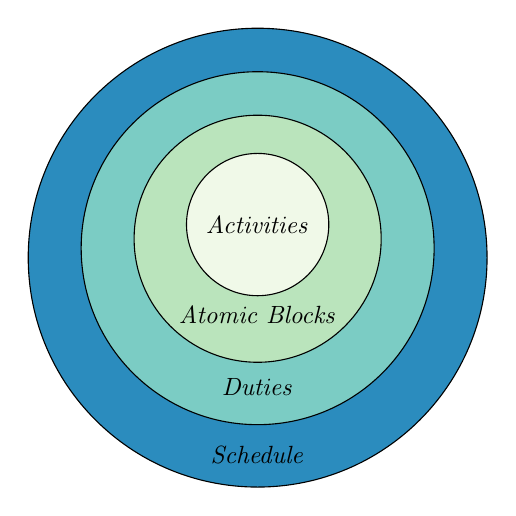
\begin{tikzpicture}[scale=0.6, every node/.style={scale=0.9}]
    \node[set,fill=blue4,text width=6.5cm,label={[below=148pt of rea,text opacity=1]\textit{Schedule}}] 
        (nat) at (0,-0.7)  (rea) {};
    \node[set,fill=blue3,text width=5cm,label={[below=108pt of rea,text opacity=1]\textit{Duties}}] 
      (nat) at (0,-0.5)  (rea) {};
    \node[set,fill=blue2,text width=3.5cm,label={[below=66pt of int]\textit{Atomic Blocks}}] 
      (int) at (0,-0.3)  {};
    \node[set,fill=blue1,text width=2cm] (nat) at (0,0) {\textit{Activities}};
    \end{tikzpicture}}%picture #1
    \qquad
    %picture #2
    \subfloat[Structure of a Duty, showing $Activities$ ($A_{i}$) inside $Atomic \; Blocks$ which themselves are inside a $Duty$.]{\raisebox{5em}{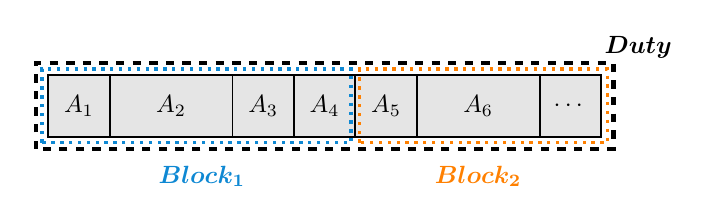
\begin{tikzpicture}[line width=.7pt,scale=0.78, every node/.style={scale=0.9}]
        %Activities
        \draw[fill=gray!20] (0,0)node[below]{} rectangle(1,1);
        %%%%%%%%%%%%%%%%%%%%%%%%%%%%%% NOTATION %%%%%%%%%%%%%%%%%%%
        %%%%%%%%%%%%%%%%%%%%%(bottomleft)             (topright)
        \draw[fill=gray!20] (1,0)node[below]{} rectangle(3,1);
        \draw[fill=gray!20] (3,0)node[below]{}rectangle(4,1);
        \draw[fill=gray!20] (4,0)node[below]{}rectangle (5,1)(2.5,1)node[below,yshift=-1.15cm, text=cyan!70!blue]{$\boldsymbol{Block_1}$};
        \draw[fill=gray!20] (5,0)node[below]{}rectangle (6,1);
        \draw[fill=gray!20] (6,0)node[below]{}rectangle (8,1);
        \draw[fill=gray!20] (8,0)node[below]{}rectangle (9,1)(7,1)node[below,yshift=-1.15cm, text=orange]{$\boldsymbol{Block_2}$}(9.605,0.75)node[below,yshift=0.9cm]{$\boldsymbol{Duty}$};
        %Blocks
        %\draw[fill=none, double=gray!40,double distance =1pt] (-0.1,-0.1)node[below]{} rectangle(4.93,1.1);
        %\draw[fill=none, double=red,double distance =1pt] (5.07,-0.1)node[below]{} rectangle(9.1,1.1);
        \draw[fill=none,very thick,dotted,draw=cyan!70!blue] (-0.1,-0.1)node[below]{} rectangle(4.93,1.1);
        \draw[fill=none,very thick,dotted,draw=orange] (5.07,-0.1)node[below]{} rectangle(9.1,1.1);
        %Duty
        \draw[fill=none,ultra thick,dashed] (-0.2,-0.2)node[below]{} rectangle(9.2,1.2);
        
        \path (0.5,.5)node{$A_1$} (2,.5)node{$A_2$} (3.5,.5)node{$A_3$} (4.5,.5)node{$A_4$} (5.5,.5)node{$A_5$} (7,.5)node{$A_6$} (8.5,.5)node{$\dotsi$};
        %%%%%%%(width of label, height)
        \end{tikzpicture}}}
    %end of picture #2
    \caption{Illustrations explaining the nature of the Input Parameters of the problem.}%
    \label{fig:Useful Time}%
\end{figure}

\vspace{\baselineskip}
\noindent
We now focus on two simplified examples that are meant to give the reader a more practical overview of the problem in question. We start off with a dreamt-up example that serves as an illustration that hopefully highlights the foundations of the problem, then transitioning to a more reality-based example that is meant to resemble what typically occurs in a Royal Mail MC.


%%%%%%%%%%%%%%%%%%%%%%%%%%%%%%%%%%%%%%%%%%%%%%%%%%%%%%%%%%%%%%%%%%%%%% Figure %%%%%%%%%%%%%%%%%%%%%%%%%%%%%%%%%%%%%%%%%%%%%%%

\begin{figure}[htb!]
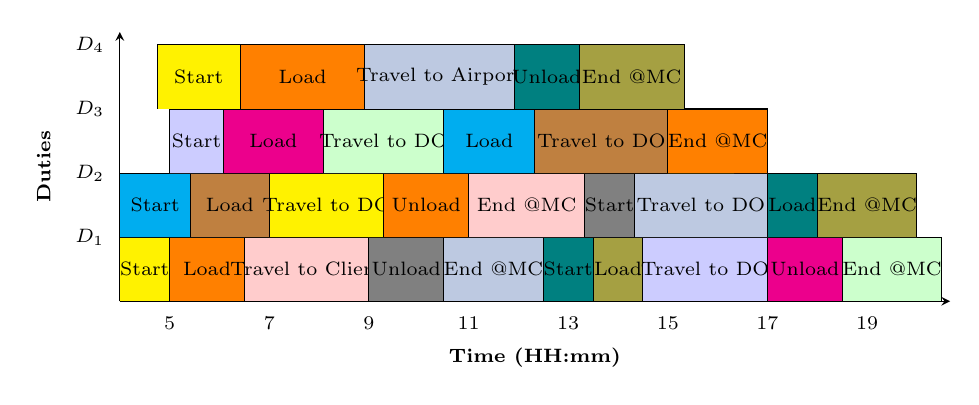
\begin{tikzpicture}
\begin{axis}[
  font=\scriptsize,
  ytick style={draw=none},
  xtick style={draw=none},
  %unit vector ratio*=1 1 1,%1 0.6 1,
  axis lines = middle,
  enlarge x limits = {value=.01,upper},
  enlarge y limits = {value=.05,upper},
  ylabel={\textbf{Duties}},
  xlabel={\textbf{Time (HH:mm)}},
  ylabel near ticks,
  xlabel near ticks,
  const plot,
  stack plots=false,
  area style,
  width=\linewidth,
  height=5cm, %control the height of chart
  %width=\linewidth,height=\textheight,
  ytick={1,...,60},
  yticklabels={},  
  xtick={1,3,...,24},
  %xticklabels = {4,6,8},
  extra y ticks={1,2,3,4},
  extra y tick style={yticklabel={$D_{\pgfmathprintnumber{\tick}}$}}
  ] 
  
  const char *colour[12] = { "yellow", "orange", "red!20", "gray", "light blue", "teal", "yellow!60!black", "blue!20", "magenta", "green!20","cyan","brown"};
  
\addplot[fill=yellow] coordinates {(4.00,0) (4.00,1) (5,1) (5,0) } node at (current path bounding box.center) {Start};
\addplot[fill=orange] coordinates {(5,0) (5,1) (6.5,1) (6.5,0) } node at (current path bounding box.center) {Load};
\addplot[fill=red!20] coordinates {(6.5,0) (6.5,1) (9.00,1) (9.00,0) } node at (current path bounding box.center) {Travel to Client};
\addplot[fill=gray] coordinates {(9.00,0) (9.00,1) (10.50,1) (10.50,0) } node at (current path bounding box.center) {Unload};
\addplot[fill=light blue] coordinates {(10.5,0) (10.5,1) (12.5,1) (12.5,0) } node at (current path bounding box.center) {End @MC};
\addplot[fill=teal] coordinates {(12.5,0) (12.5,1) (13.5,1) (13.5,0) } node at (current path bounding box.center) {Start};
\addplot[fill=yellow!60!black] coordinates {(13.5,0) (13.5,1) (14.5,1) (14.5,0) } node at (current path bounding box.center) {Load};
\addplot[fill=blue!20] coordinates {(14.5,0) (14.5,1) (17.00,1) (17.00,0) } node at (current path bounding box.center) {Travel to DO};
\addplot[fill=magenta] coordinates {(17.00,0) (17.00,1) (18.50,1) (18.50,0) } node at (current path bounding box.center) {Unload};
\addplot[fill=green!20] coordinates {(18.5,0) (18.5,1) (20.5,1) (20.5,0) } node at (current path bounding box.center) {End @MC};
\addplot[fill=cyan] coordinates {(4.00,1) (4.00,2) (5.42,2) (5.42,1) } node at (current path bounding box.center) {Start};
\addplot[fill=brown] coordinates {(5.42,1) (5.42,2) (7,2) (7,1) } node at (current path bounding box.center) {Load};
\addplot[fill=yellow] coordinates {(7,1) (7,2) (9.30,2) (9.30,1) } node at (current path bounding box.center) {Travel to DO};
\addplot[fill=orange] coordinates {(9.3,1) (9.3,2) (11,2) (11,1) } node at (current path bounding box.center) {Unload};
\addplot[fill=red!20] coordinates {(11,1) (11,2) (13.33,2) (13.33,1) } node at (current path bounding box.center) {End @MC};
\addplot[fill=gray] coordinates {(13.33,1) (13.33,2) (14.33,2) (14.33,1) } node at (current path bounding box.center) {Start};
\addplot[fill=light blue] coordinates {(14.33,1) (14.33,2) (17,2) (17,1) } node at (current path bounding box.center) {Travel to DO};
\addplot[fill=teal] coordinates {(17,1) (17,2) (18,2) (18,1) } node at (current path bounding box.center) {Load};
\addplot[fill=yellow!60!black] coordinates {(18,1) (18,2) (20,2) (20,1) } node at (current path bounding box.center) {End @MC};
\addplot[fill=blue!20] coordinates {(5.00,2) (5.00,3) (6.08,3) (6.08,2) } node at (current path bounding box.center) {Start};
\addplot[fill=magenta] coordinates {(6.08,2) (6.08,3) (8.08,3) (8.08,2) } node at (current path bounding box.center) {Load};
\addplot[fill=green!20] coordinates {(8.08,2) (8.08,3) (10.50,3) (10.50,2) } node at (current path bounding box.center) {Travel to DO};
\addplot[fill=cyan] coordinates {(10.50,2) (10.50,3) (12.33,3) (12.33,2) } node at (current path bounding box.center) {Load};
\addplot[fill=brown] coordinates {(12.33,2) (12.33,3) (15,3) (15,2) } node at (current path bounding box.center) {Travel to DO};
\addplot[fill=yellow] coordinates {(15,2) (15,3) (16.33,3) (16.33,2) } node at (current path bounding box.center) {Unload};
\addplot[fill=orange] coordinates {(15,2) (15,3) (17,3) (17,2) } node at (current path bounding box.center) {End @MC};
\addplot[fill=yellow] coordinates {(4.75,3) (4.75,4) (6.42,4) (6.42,3) } node at (current path bounding box.center) {Start};
\addplot[fill=orange] coordinates {(6.42,3) (6.42,4) (8.92,4) (8.92,3) } node at (current path bounding box.center) {Load};
\addplot[fill=light blue] coordinates {(8.92,3) (8.92,4) (11.92,4) (11.92,3) } node at (current path bounding box.center) {Travel to Airport};
\addplot[fill=teal] coordinates {(11.92,3) (11.92,4) (13.22,4) (13.22,3) } node at (current path bounding box.center) {Unload};
\addplot[fill=yellow!60!black] coordinates {(13.22,3) (13.22,4) (15.33,4) (15.33,3) } node at (current path bounding box.center) {End @MC};
\end{axis}
\end{tikzpicture}
    \caption{Gantt chart of abstract exemplary case.}
    \label{fig:Schedule-for-abstract-exemplary-case}
\end{figure}

%%%%%%%%%%%%%%%%%%%%%%%%%%%%%%%%%%%%%%%%%%%%%%%%%%%%%%%%%%%%%%%%%%%%%% sub-Section %%%%%%%%%%%%%%%%%%%%%%%%%%%%%%%%%%%%%%%%%%%%%%%

\subsection*{Generalised Schedule Template}
We start with an abstracted example that resembles our problem very closely. The goal of this section is to formalise the problem and give the reader a general sense of the specifics of the problem. We have a set of duties and a set of blocks. In particular, we have 4 duties at our disposal and 6 atomic blocks that require scheduling. The details of the blocks schedule in each of the four duties are seen in the table below:

\begin{table}[h]
\small
    \centering 
    \begin{tabular}{|c|c|c|c|c|}
        \hline
        \textbf{Block} & \multicolumn{4}{|c|}{ \textbf{Characteristics}} \\
        \hline
        & Start Time & End Time & Number of Activities & Perfored by Duty\\
        \hline
        1 & 04:00 & 12:30 & 5 & 1\\
        \hline
        2 & 12:30 & 20:30 & 5 & 1\\
        \hline
        3 & 04:00 & 13:20  & 5 & 2\\
        \hline
        4 & 13:20 & 20:00 & 4 & 2\\
        \hline
        5 & 05:00 & 17:00 & 6 & 3\\
        \hline
        6 & 04:45 & 15:20 & 5 & 4\\
        \hline
    \end{tabular}%
    \medbreak
\end{table}
%of activities. (or maybe a real small instance of  Royal Mail, to say oh for example this is what happened in Royal στο πρώτο wave της %Δευτέρας, και write for confidentiality purposes we call them ATOMIC BLOCK 1,2,4, 5 or Athens, Tripoli, Thessaloniki Or do both actually).

\vspace{\baselineskip}
\noindent
In this particular example we show the process of creating a schedule through an instance of blocks and duties. Namely, the act of scheduling is to place the blocks inside duties in a particular sequence. In this case that sequence is performed heuristically without the help of an algorithm.

\vspace{\baselineskip}
\noindent
Nonetheless certain interesting facts can be determined from this example. To start with, we can see that the \texttt{End} activity incorporates the travel leg from the external location back to the MC. Moreover, we can see that the length of the trip back to the MC is more often than not shorter than that of the trip to the external location. This is observed, because usually the initial travel leg from the MC is conducted during rush hours since the mail needs to be delivered first thing in the morning. In contrast the travel leg back to the MC is not particularly rushed and the driver can determine the best time to complete it. 

\vspace{\baselineskip}
\noindent
The typical blocks that occur most often are blocks such as block 1-3. They contain the typical sequence of activities: the \texttt{start} to the duty, the \texttt{loading} of the mail, the \texttt{travel leg} to the external location after the \texttt{unloading} of the mail a return back to the MC to \texttt{end} the duty. In contrast  blocks 4-6 are slightly unique in their sequence of events. Block number 4 for instance is a \textit{container repatriation trip}. The HGV leaves the MC to pick up containers that were previously left at an external location, in order to bring the back to the MC for their use the following day.


%%%%%%%%%%%%%%%%%%%%%%%%%%%%%%%%%%%%%%%%%%%%%%%%%%%%%%%%%%%%%%%%%%%%%% sub-Section %%%%%%%%%%%%%%%%%%%%%%%%%%%%%%%%%%%%%%%%%%%%%%%

\subsection*{Historical Schedule Example}
We present an isolated version of our problem that only concerns a small part of the overall problem. The thought process behind this example is to simulate for the reader what typically occurs in a Royal Mail MC. More specifically, we present part of the schedule that dictates the Monday morning operations at a MC. This is illustrated through a Gantt chart in Figure \ref{fig:Schedule-for-exemplary-case} which aims to highlight a small snippet of what would occur in a MC at the start of a week.

\vspace{\baselineskip}
\noindent
Taking a more detailed look one can see that maybe this historical schedule is \textbf{not so balanced}. The majority of people look like they work for around 8 hours such as the first shift ($D_1$) that began at 4:00 AM and concluded at 12:00 PM. For confidentiality purposes, the names of locations, clients, and jobs undertaken by each drivers have been omitted and generic placeholder names have been used instead. For instance,  shift $D_1$  consisted of 4 \textbf{atomic blocks}, hence 4 \textbf{round-trips}. The first atomic block, is the largest one in this duty and consisted of visiting 6 external locations, after the start of the trip from the MC. Following, that 3 smaller atomic blocks that consisted of short-lasting round trips were completed by this driver, until h(er)is end of the duty.

\vspace{\baselineskip}
\noindent
However, taking a more macro outlook on this schedule we can see that there are also people who are required to do overtimes which might be costly for the company,  such as shift ($D_{14}$) that begins at 5:00 AM and lasts until 5:00 PM. This particular shift, consisted of \textbf{6 atomic blocks}, where the first one, was also a fairly long-lasting one. It could be possible to obtain a more uniform allocation of blocks per driver, that would result in a more uniform allocation of workload. That is the purpose of the experiments, we then run in Chapter \ref{chapter: 2-Evaluating Royal Mail Historical Data}.

%%%%%%%%%%%%%%%%%%%%%%%%%%%%%%%%%%%%%%%%%%%%%%%%%%%%%%%%%%%%%%%%%%%%%% Figure %%%%%%%%%%%%%%%%%%%%%%%%%%%%%%%%%%%%%%%%%%%%%%%

\begin{figure}
\begin{tikzpicture}
\begin{axis}[
  font=\footnotesize,
  ytick style={draw=none},
  xtick style={draw=none},
  unit vector ratio*=1 1 1,
  axis lines = middle,
  enlarge x limits = {value=.01,upper},
  enlarge y limits = {value=.05,upper},
  ylabel={\textbf{Duties}},
  xlabel={\textbf{Time (HH:mm)}},
  ylabel near ticks,
  xlabel near ticks,
  const plot,
  stack plots=false,
  area style,
  width=\linewidth,height=\textheight,
  ytick={1,...,60},
  yticklabels={},  
  xtick={1,...,24},
  extra y ticks={1,2,3,4,5,6,7,8,9,10,11,12,13,14},
  extra y tick style={yticklabel={$D_{\pgfmathprintnumber{\tick}}$}}
  ] 
\addplot[fill=yellow] coordinates {(4.00,0) (4.00,1) (8.08,1) (8.08,0) } node at (current path bounding box.center) {B1};
\addplot[fill=orange] coordinates {(8.08,0) (8.08,1) (8.83,1) (8.83,0) } node at (current path bounding box.center) {B2};
\addplot[fill=red!20] coordinates {(8.83,0) (8.83,1) (11.00,1) (11.00,0) } node at (current path bounding box.center) {B3};
\addplot[fill=gray] coordinates {(11.00,0) (11.00,1) (11.92,1) (11.92,0) } node at (current path bounding box.center) {B4};
\addplot[fill=light blue] coordinates {(4.00,1) (4.00,2) (7.42,2) (7.42,1) } node at (current path bounding box.center) {B1};
\addplot[fill=teal] coordinates {(7.42,1) (7.42,2) (12.33,2) (12.33,1) } node at (current path bounding box.center) {B2};
\addplot[fill=yellow!60!black] coordinates {(4.00,2) (4.00,3) (6.08,3) (6.08,2) } node at (current path bounding box.center) {B1};
\addplot[fill=blue!20] coordinates {(6.08,2) (6.08,3) (8.08,3) (8.08,2) } node at (current path bounding box.center) {B2};
\addplot[fill=magenta] coordinates {(8.08,2) (8.08,3) (10.50,3) (10.50,2) } node at (current path bounding box.center) {B3};
\addplot[fill=green!20] coordinates {(10.50,2) (10.50,3) (12.33,3) (12.33,2) } node at (current path bounding box.center) {B4};
\addplot[fill=yellow] coordinates {(4.00,3) (4.00,4) (6.42,4) (6.42,3) } node at (current path bounding box.center) {B1};
\addplot[fill=orange] coordinates {(6.42,3) (6.42,4) (8.92,4) (8.92,3) } node at (current path bounding box.center) {B2};
\addplot[fill=red!20] coordinates {(8.92,3) (8.92,4) (11.33,4) (11.33,3) } node at (current path bounding box.center) {B3};
\addplot[fill=gray] coordinates {(4.00,4) (4.00,5) (5.33,5) (5.33,4) } node at (current path bounding box.center) {B1};
\addplot[fill=light blue] coordinates {(5.33,4) (5.33,5) (7.83,5) (7.83,4) } node at (current path bounding box.center) {B2};
\addplot[fill=teal] coordinates {(7.83,4) (7.83,5) (8.50,5) (8.50,4) } node at (current path bounding box.center) {B3};
\addplot[fill=yellow!60!black] coordinates {(8.50,4) (8.50,5) (11.25,5) (11.25,4) } node at (current path bounding box.center) {B4};
\addplot[fill=blue!20] coordinates {(4.00,5) (4.00,6) (6.22,6) (6.22,5) } node at (current path bounding box.center) {B1};
\addplot[fill=magenta] coordinates {(6.22,5) (6.22,6) (8.72,6) (8.72,5) } node at (current path bounding box.center) {B2};
\addplot[fill=green!20] coordinates {(8.72,5) (8.72,6) (11.88,6) (11.88,5) } node at (current path bounding box.center) {B3};
\addplot[fill=yellow] coordinates {(4.00,6) (4.00,7) (6.58,7) (6.58,6) } node at (current path bounding box.center) {B1};
\addplot[fill=orange] coordinates {(6.58,6) (6.58,7) (9.17,7) (9.17,6) } node at (current path bounding box.center) {B2};
\addplot[fill=red!20] coordinates {(9.17,6) (9.17,7) (11.67,7) (11.67,6) } node at (current path bounding box.center) {B3};
\addplot[fill=gray] coordinates {(4.00,7) (4.00,8) (6.50,8) (6.50,7) } node at (current path bounding box.center) {B1};
\addplot[fill=light blue] coordinates {(6.50,7) (6.50,8) (8.50,8) (8.50,7) } node at (current path bounding box.center) {B2};
\addplot[fill=teal] coordinates {(8.50,7) (8.50,8) (11.67,8) (11.67,7) } node at (current path bounding box.center) {B3};
\addplot[fill=green!20] coordinates {(4.00,8) (4.00,9) (7.50,9) (7.50,8) } node at (current path bounding box.center) {B1};
\addplot[fill=yellow] coordinates {(7.50,8) (7.50,9) (8.83,9) (8.83,8) } node at (current path bounding box.center) {B2};
\addplot[fill=orange] coordinates {(8.83,8) (8.83,9) (10.50,9) (10.50,8) } node at (current path bounding box.center) {B3};
\addplot[fill=red!20] coordinates {(10.50,8) (10.50,9) (12.50,9) (12.50,8) } node at (current path bounding box.center) {B4};
\addplot[fill=gray] coordinates {(4.50,9) (4.50,10) (7.83,10) (7.83,9) } node at (current path bounding box.center) {B1};
\addplot[fill=light blue] coordinates {(7.83,9) (7.83,10) (9.67,10) (9.67,9) } node at (current path bounding box.center) {B2};
\addplot[fill=teal] coordinates {(9.67,9) (9.67,10) (12.17,10) (12.17,9) } node at (current path bounding box.center) {B3};
\addplot[fill=orange] coordinates {(12.17,9) (12.17,10) (14.08,10) (14.08,9) } node at (current path bounding box.center) {B4};
\addplot[fill=yellow!60!black] coordinates {(4.50,10) (4.50,11) (8.42,11) (8.42,10) } node at (current path bounding box.center) {B1};
\addplot[fill=blue!20] coordinates {(8.42,10) (8.42,11) (12.08,11) (12.08,10) } node at (current path bounding box.center) {B2};
\addplot[fill=magenta] coordinates {(12.08,10) (12.08,11) (13.00,11) (13.00,10) } node at (current path bounding box.center) {B3};
\addplot[fill=green!20] coordinates {(4.50,11) (4.50,12) (7.05,12) (7.05,11) } node at (current path bounding box.center) {B1};
\addplot[fill=yellow] coordinates {(7.05,11) (7.05,12) (9.05,12) (9.05,11) } node at (current path bounding box.center) {B2};
\addplot[fill=orange] coordinates {(9.05,11) (9.05,12) (12.88,12) (12.88,11) } node at (current path bounding box.center) {B3};
\addplot[fill=red!20] coordinates {(5,12) (5,13) (7.25,13) (7.25,12) } node at (current path bounding box.center) {B1};
\addplot[fill=gray] coordinates {(7.25,12) (7.25,13) (10.67,13) (10.67,12) } node at (current path bounding box.center) {B2};
\addplot[fill=light blue] coordinates {(10.67,12) (10.67,13) (13.83,13) (13.83,12) } node at (current path bounding box.center) {B3};
\addplot[fill=teal] coordinates {(5.15,13) (5.15,14) (9.08,14) (9.08,13) } node at (current path bounding box.center) {B1};
\addplot[fill=yellow] coordinates {(9.08,13) (9.08,14) (11.50,14) (11.50,13) } node at (current path bounding box.center) {B2};
\addplot[fill=orange] coordinates {(11.50,13) (11.50,14) (12.50,14) (12.50,13) } node at (current path bounding box.center) {B3};
\addplot[fill=red!20] coordinates {(12.50,13) (12.50,14) (13.30,14) (13.30,13) } node at (current path bounding box.center) {B4};
\addplot[fill=gray] coordinates {(13.30,13) (13.30,14) (15.08,14) (15.08,13) } node at (current path bounding box.center) {B5};
\addplot[fill=magenta] coordinates {(15.08,13) (15.08,14) (17.08,14) (17.08,13) } node at (current path bounding box.center) {B6};
\end{axis}
\end{tikzpicture}
    \caption{Gantt chart showing \textit{Blocks} ($B_j$) allocated to \textit{Duties} ($D_i$) as in the Monday morning schedule of the MC.}
    \label{fig:Schedule-for-exemplary-case}
\end{figure}

%%%%%%%%%%%%%%%%%%%%%%%%%%%%%%%%%%%%%%%%%%%%%%%%%%%%%%%%%%%%%%%%%%%%%% Section %%%%%%%%%%%%%%%%%%%%%%%%%%%%%%%%%%%%%%%%%%%%%%%

\section{Dataset Exploration}
\label{section: Data Exploration}
Royal Mail have provided historical data from the Exeter MC, that shows the itineraries that the HGV drivers follow over a week. Namely, a \textbf{model week} that represents the normal \textbf{mode of operation} of a Royal Mail MC over a typical week of the year. The main data points featured in the dataset stem from the Input Parameters outlined in Section \ref{section: Input Parameters}, and below we mention the attributes associated with each \textit{Input Parameter} from within the dataset:

%%%%%%%%%%%%%%%%%%%%%%%%%%%%%%%%%%%%%%%%%%%%%%%%%%%%%%%%%%%%%%%%%%%%%% Bullet points %%%%%%%%%%%%%%%%%%%%%%%%%%%%%%%%%%%%%%%%%%%%%%%

\begin{itemize}
    \item \underline{\textbf{Activity}}: Each unit of activity is described by a \textit{tuple}\textit{ a/b/c/d}, where \textit{a}, \textit{b} are the origin and destination locations where the activity takes place, and \textit{c}, \textit{d} are its \texttt{start} and \texttt{end} time. The difference $|d-c|$ therefore, shows the \texttt{duration} or \texttt{processing time} of the activity. 
    
    \item \underline{\textbf{Atomic Interval (block)}}: In the dataset, a \textbf{block} is constituted by a set of \textbf{activities} from table \ref{table:Activity List}. We identify a block by its first, and last activity, and more specifically merely by the \texttt{start}, and \texttt{end} time of the \texttt{start/end} activity since the locations at the start and end will be the MC itself, by the definition of a block.
    
    \todo{Figure required showing this thing with first and last start/end activity.}
    
        \item \underline{\textbf{Duty}}: The largest unit of time seen in the dataset that consists of a collection of \textbf{blocks}. Duties in the dataset correspond to a \textit{driver} taking the \textit{HGV} assigned to them, and completing the collection of \textbf{blocks} (i.e. round-trips) required.
\end{itemize}

\vspace{\baselineskip}
\noindent
The historical schedules in the dataset, are the current feasible itineraries that Royal Mail operates. After careful analysis of the \textbf{200} duties in the dataset, we can infer that the Exeter MC serves 30 DOs,  38 client locations with a fleet of  65 total HGVs split between 17, 7.5 tonne lorries, and 3.5 tonne vans. Moreover, we deduce that the Exeter MC opens for business at 4:00 AM in the morning on all weekdays, as well as on Saturday.  Sunday is an exception, with a single shift commencing at 8:00 AM and finishing at 6:00 PM in the afternoon. The \textbf{absolute latest finishing time} of a shift for weekdays as well as for Saturday is at 3:00 AM in the morning which constitutes the \textit{close of business (COB)} for the day. The tuning of the absolute \textbf{earliest starting time} and \textbf{latest finishing time} are two of the most important optimisation decisions to be made since, opening for business slightly earlier than the current 4:00 AM time set by company policy, could result in an overall reduction of the duration of the each day's schedule.

%%%%%%%%%%%%%%%%%%%%%%%%%%%%%%%%%%%%%%%%%%%%%%%%%%%%%%%%%%%%%%%%%%%%%% Table %%%%%%%%%%%%%%%%%%%%%%%%%%%%%%%%%%%%%%%%%%%%%%%

\begin{table}[t]
\small
    \centering 
    \begin{tabular}{|c|c|c|c|c|c|c|c|}
        \hline
        \textbf{Schedule} & \multicolumn{3}{|c|}{ \textbf{Characteristics}} & \multicolumn{3}{|c|}{ \textbf{Duties (HH:mm)}} & \textbf{Total Time}  \\
        \hline
        & Duties & Blocks & Activities & Average &  Minimum & Makespan & \\
        \hline
        Original & 200 & 514 & 3,555 & 07:50 & 02:50 & 11:50 & 1,657:51 \\
        \hline
    \end{tabular}%
    \medbreak
\end{table}

\vspace{\baselineskip}
\noindent
Taking a closer look at the idiosyncrasies of the current set of schedules we can extract the following \textbf{insights} for each class of activities:

\vspace{\baselineskip}

%%%%%%%%%%%%%%%%%%%%%%%%%%%%%%%%%%%%%%%%%%%%%%%%%%%%%%%%%%%%%%%%%%%%%% Bullet Points %%%%%%%%%%%%%%%%%%%%%%%%%%%%%%%%%%%%%%%%%%%%%%%

\begin{enumerate}
    
    \item \underline{\texttt{Start/End}}: Duties tend to begin in a wave-like fashion. We observed three waves of starting times, with waves occurring near the opening of business, midnight and mid-day\footnote{Detailed evidence from the dataset highlighting this phenomenon can be seen in Figure \ref{fig:starting time} of Appendix \ref{subsection: Appendix Starting times}}. The drivers are split in those three groups, with approximately 59 drivers beginning their shift in the \textbf{morning} wave and 61, 63 in the \textbf{afternoon} and \textbf{night} waves respectively.  
    
    \item \underline{\texttt{Travel}}: For each, of the travel activities, we are also supplied with data regarding the mileage covered during each trip as well as, a description regarding the reason for that leg of the trip (e.g. mail, time-sensitive mail, repatriation of mail containers etc.). Leveraging this attribute of travel legs we can see that a certain subset of atomic blocks that contain time-critical tasks occurring within a certain time-span of the day tend to take place at the beginning of a duty. These are the blocks containing the \textit{delivery} of post itself as well as, delivery of time-critical parcels to the airport. In contrast, other blocks that involve non-time-constrained tasks for example \textit{container repatriation} or when an HGV returns with an \textit{empty} cargo bay following a delivery, can be scheduled interchangeably within a shift, and are hence more open to optimisation.
    
    \item \underline{\texttt{Load/Unload}}: A \textit{load/unload} activity takes place, immediately prior and directly subsequent of a travel leg, as illustrated in Figure \ref{fig:load/unload}. Although this activity  could be considered non-useful time as it is time not spent on the road, it cannot nonetheless be optimised away, since company policy states that the driver must be present, and should not be occupied with any other activity in parallel to a \texttt{load/unload} of the mail units. Consequently, for the purposes of our optimisation problem we consider this to be \textbf{useful} time.  
    
    \item \underline{\texttt{Meal-Relief}}: The meal allowance occurs immediately before or after the beginning or end of a block. It is freely interchangeable within the space of a duty but given that it must occur at the premises of the MC, it always occurs at the start or at the end of a block.        
    
    \item \underline{\texttt{Processing/Distribution}}: There are cases when a gap occurs between two activities due to the finishing time of the prior activity not completely coinciding with the starting time of the following one. Given that both activities are rigidly scheduled in place and cannot be altered to coincide, drivers are heuristically instructed to fill in the time until their next \textit{useful} activity by assisting with administrative tasks that ideally should be carried out by lower-skilled employees. As a result, unnecessary costs are incurred by Royal Mail due to the inefficiency of the schedule. These activities provide us with the opportunity to minimise the makespan of each duty by attempting to reduce their rate of occurrence, as seen in Section \ref{section: Redefined Dataset}. 
   
    \item \underline{\texttt{Park Vehicle}}: The parking activity occurs four times within the dataset whenever a \texttt{3.5 Tonne van} arrives at the National Distribution Center. For the majority of duties, the time taken to complete the parking activity is incorporated in the duration of the End activity. It is only in these four duties that parking is included as a separate activity. As a result, we can assume that we can incorporate it ourselves into the \texttt{End} activity in those four duties to simplify the dataset as a whole, and equivalently then render the \textt{Park Vehicle} activity as \textbf{non-useful} time.
    
    \item \underline{\texttt{Check}}: They occur  as standalone activities in a handful of shifts that are carried out by the \texttt{3.5 Tonne Vans}. In the majority of cases they are included in the time that the \texttt{Start} activity takes, as explained by the description attached to each activity. As a result, they occur at the beginning of each duty, and tend to take less than 25 minutes. Hence, similarly to the \textt{Park Vehicle} activity, we can incorporate them into the \textt{Start} activity, and characterise \texttt{Check} as \textbf{non-useful}.
    
    \item \underline{\texttt{Clean}}: These take place at the \textit{beginning} or \textit{end} of blocks, and after more critical activities have been completed. For example, if a \texttt{Meal-Relief} and a \texttt{Clean} are both scheduled to take place exactly at the end of a block, priority will be given to the \texttt{Meal-Relief}, since it is a more time sensitive activity. In the majority of cases, it is not entered as a standalone entry and is described as part of the time taken for \texttt{Start} or \textit{End} activities. 
\end{enumerate}

%%%%%%%%%%%%%%%%%%%%%%%%%%%%%%%%%%%%%%%%%%%%%%%%%%%%%%%%%%%%%%%%%%%%%% Figure %%%%%%%%%%%%%%%%%%%%%%%%%%%%%%%%%%%%%%%%%%%%%%%

\begin{figure}{
\centering
    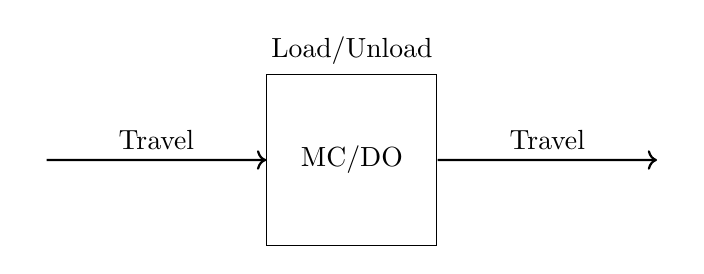
\begin{tikzpicture}[square/.style={regular polygon,regular polygon sides=4}]
        \node (A) at (0,0){};
        \node (B) at (4,0) [square,draw,label=above:{Load/Unload}]  {MC/DO};
        \draw[thick,->] (A) -- (B) node[midway,above] {Travel};
        \node (C) at (8,0){};
        \draw[thick,->] (B) -- (C) node[midway,above] {Travel};
        
    \end{tikzpicture}
           
    \caption{Illustration of the pattern of activities that directly succeeds and precedes any travel-leg of an atomic interval.}
    \label{fig:load/unload}
    }\end{figure}

%%%%%%%%%%%%%%%%%%%%%%%%%%%%%%%%%%%%%%%%%%%%%%%%%%%%%%%%%%%%%%%%%%%%%% Section %%%%%%%%%%%%%%%%%%%%%%%%%%%%%%%%%%%%%%%%%%%%%%%

\section{Data Cleaning}
\label{section: Data Cleaning}
The quality and effectiveness of the schedules that we hope to generate, will depend significantly on the quality of the dataset from which our schedules will be derived. Consequently, an extensive process to clean the dataset from outliers and general noise is undertaken with the goal of filtering down the schedules to show the most frequently occurring duties which accurately depict what typically occurs in a MC such that an optimisation would really make a difference to Royal Mail.\par

\vspace{\baselineskip}
\noindent
To retain the reproducibility of the dataset, the specific steps that were taken to clean the dataset are outlined below:

%%%%%%%%%%%%%%%%%%%%%%%%%%%%%%%%%%%%%%%%%%%%%%%%%%%%%%%%%%%%%%%%%%%%%% Bullet points %%%%%%%%%%%%%%%%%%%%%%%%%%%%%%%%%%%%%%%%%%%%%%%

\vspace{\baselineskip}
\begin{enumerate}[label=\textbf{\arabic*}.]

\item \underline{\textbf{Elimination of unwanted attributes}}: The dataset contained numerous attributes attached to each activity, that are utilised in accordance with internal company policy. For instance, some of those attributes contained information regarding the level of driving skills required for each duty. However, our problem operates within the context of \textit{multiprocessor scheduling}, where all machines are considered to be identical, and is hence agnostic to the level of skill of the HGV drivers. We view each task as if it is processed by a machine so we choose to neglect the information provided by those fields and focus merely on scheduling \textbf{legal} and \textbf{feasible} duties. Consequently, the following fields were eliminated from our dataset \texttt{driver\_grade, sort\_order, date\_amended}. A more detailed list of the attributes contained in the dataset can be seen in Appendix \ref{section: Appendix Activities Feaure in the Dataset}.


\item \underline{\textbf{Incorporation of sparsely occurring activities into \texttt{Start} and \texttt{End} activities}}: Within the dataset, we observed that the parking activity occurs on its own, in only a handful of cases and is instead incorporated into the \texttt{End} activity in the majority of cases (as we were informed by the description of the task undertaken, attached to some of the activities). Hence, to avoid focusing on \textbf{unwanted} noise cases, we chose to incorporate the duration of the parking activity into the end activity for those cases. In a similar fashion we include, \texttt{Clean} and \texttt{Check} to the \texttt{Start}, and \texttt{End} activities as is appropriate.


\item \underline{\textbf{Standardisation of standalone entries}}: In a small subset of cases, an extra level of detail is added onto the duties specifying whether a \texttt{load} or \texttt{unload} activity is being undertaken as opposed to labelling it as a more general \texttt{load/unload} operation. Given, that this extra layer of detail does not concurrently add any extra level of understanding to the problem we choose to label all separate \texttt{load} and \texttt{unload} operations as a more abstract \texttt{load/unload} activity. The same procedure is carried out for separate entries of \texttt{Processing}, and \texttt{Distribution} activities the distinction of which is similarly of no significance to us.\par


\item \underline{\textbf{Neglected duties that involve trips to out-of-scope Royal Mail premises}}: Our focus is placed on optimising the scheduling of the routes that occur between the Exeter MC, and the DOs as well as clients for which it is responsible. Hence, duties that involve trips to the \textit{Distribution Centres} and other MCs are out of our scope for optimisation, hence we do not consider trips to those locations.\par


\item \underline{\textbf{Elimination of Outliers}}: We did not consider entries that involved duties finishing after the \textit{close of business (COB)} as we assumed they involve out of the ordinary situations where duties run late and hence, do not reflect normal business practice.\par


\item \underline{\textbf{Neglected data related to Time-Constrained mail}}: We ignore data that is related to \textbf{time-constrained packages}, as the modelling of such block is out of scope for this project. This decision was made in conjunction with the Royal Mail Data Science group, since the study of such specific trips was not at the time the top priority. The thought process behind this action is that for the purposes of our project we want total freedom as far as moving the blocks and these duties reflect \textbf{fixed blocks} hence, represent constraints to our optimisation problem. In practice, to avoid considering such trips occurring in the dataset that was going to be used for the modelling portion of the project, we choose to neglect duties that involve trips to the Exeter Airport, as it is such trips that often have a time-limit attached to them. \par


\item \underline{\textbf{Neglected flawed data entries}}: In a handful of duties, no presence of an atomic block was observed, instead merely activities were scheduled without a \texttt{Travel} leg that constituted the \textit{round-trip} of an \textbf{atomic block} being present. Such cases were also considered to be abnormal entries and were not taken into consideration. \par

\end{enumerate}

\vspace{\baselineskip}
\noindent
The resulting \textbf{Finalised Dataset (Cleaned)} that was obtained after subjecting the original dataset to the aforementioned data cleaning processes, schedule the activities in Table \ref{table:Final Activity List}, and has the following characteristics: 

%%%%%%%%%%%%%%%%%%%%%%%%%%%%%%%%%%%%%%%%%%%%%%%%%%%%%%% Table %%%%%%%%%%%%%%%%%%%%%%%%%%%%%%%%%%%%%%%%%%%%%%%%%%%%%%%%%%%%%%%%%%%%%%%%%%%

\begin{table}[ht]
\small
    \centering 
    \begin{tabular}{|c|c|c|c|c|c|c|c|}
        \hline
        \textbf{Schedule} & \multicolumn{3}{|c|}{ \textbf{Characteristics}} & \multicolumn{3}{|c|}{ \textbf{Duties (HH:mm)}} & \textbf{Total Time}  \\
        \hline
        & Duties & Blocks & Activities & Average &  Minimum & Makespan & \\
        \hline
        Original & 200 & 514 & 3,555 & 08:18 & 02:50 & 11:50 & 1,657:51 \\
        \hline
        Cleaned & 183 & 462 & 3,285 & 07:50 & 02:50 & 11:50 & 1,435:22 \\
        \hline
    \end{tabular}%
    \medbreak
\end{table}

%%%%%%%%%%%%%%%%%%%%%%%%%%%%%%%%%%%%%%%%%%%%%%%%%%%%%%%%%%%%%%%%%%%%%% Table %%%%%%%%%%%%%%%%%%%%%%%%%%%%%%%%%%%%%%%%%%%%%%%


%Table containing the types of activities
\begin{table}[ht]
\small
    \centering 
    \begin{tabular}{|l|p{8.3cm}|}
        \hline
       \multicolumn{1}{|c|}{ \textbf{Activity}} & \multicolumn{1}{|c|}{ \textbf{Description}} \\
        \hline
        \texttt{Start/End}  & Indicates the \textit{beginning}, and \textit{end} of a duty. \\
        \hline
        \texttt{Travel}  & The \textit{travel leg} from one location to the next. \\ 
        \hline
       \multirow{2}*{\texttt{Load/Unload}}  & The \textit{loading} and \textit{offloading} of mail units before leaving or after arriving to a designated location respectively.   \\ 
        \hline
        \multirow{2}*{\texttt{Meal-Relief}}  & The \textit{meal allowance} break to meet EU \textit{driving time} regulations. \\ 
        \hline
       \texttt{Distribution/Processing}  & Non-essential administrative tasks. \\     
        \hline
        \texttt{Park Vehicle}   & \textit{Parking} of HGV at end of duty. \\ 
        \hline
        \texttt{Check}  & Scheduled \textit{servicing} of HGV. \\ 
        \hline
        \texttt{Clean}  & Scheduled \textit{cleaning} of HGV. \\ 
        \hline
    \end{tabular}%
    \medbreak
    \caption{List of activities in the \textbf{Finalised Dataset (Cleaned)}.}
    \label{table:Final Activity List}
\end{table}



%%%%%%%%%%%%%%%%%%%%%%%%%%%%%%%%%%%%%%%%%%%%%%%%%%%%%%%%%%%%%%%%%%%%%% Section %%%%%%%%%%%%%%%%%%%%%%%%%%%%%%%%%%%%%%%%%%%%%%%

\section{Eliminating Redundant Activities}
\label{section: Redefined Dataset}
The finalised dataset presented above will be used to solve models that will provide us with a primary level of understanding in regards to the opportunities for optimisation. We then decided to artificially create some more space for optimisation in the historical data by implementing the first step in the procedures implemented on a daily basis by Royal Mail Scheduling operators to create the actual schedules utilised in MCs. That step involves neglecting activities within the atomic blocks that involve the completion of tasks considered \textbf{non-useful} time for the drivers. The activities, are generally classified in two categories, \textit{useful} and \textit{non-useful}. \textit{Useful} time for \textit{HGV} drivers, from the perspective of Royal Mail, is time related to activities during which, the driver \textbf{must be present} and \textbf{in control} of the task  (e.g. activities involving driving). On the contrary \textit{non-useful} time refers to activities that are put in place as padding time between two successive \textit{useful} activities, that have been schedule to start at a particular time. To fill the time between those \textit{useful} activities drivers end up helping with other activities that are primarily designed for employees of different specialties. 

\vspace{\baselineskip}
\noindent
The classification was performed based on the frequency with which activities occurred in the dataset. Sparsely occurring activities were labelled as \textit{non-useful} as they did not carry the vast portion of the workload and were hence deemed non critical. As a result, the activities were distinguished in accordance with Table \ref{table: Useful vs Non-Useful Activities}. The reasoning behind distinguishing the activities in this manner is to signify which activities must be maintained in place during our quest to allocate as much of the time available within a shift to \textit{useful} activities, (i.e. minimise the \textit{non-useful} time). This operation gives us the necessary space, or else \textbf{idle time} within the historical duties to re-schedule the blocks in a more efficient manner. We now have a revised historical dataset, that we refer to as \textbf{Redefined Historical Schedules}. 


%%%%%%%%%%%%%%%%%%%%%%%%%%%%%%%%%%%%%%%%%%%%%%%%%%%%%%% Double Figure %%%%%%%%%%%%%%%%%%%%%%%%%%%%%%%%%%%%%%%%%%%%%%%%%%%%%%%%%%%%%%%%%%%%%%%%%%%

\begin{figure}[ht]
\begin{floatrow}
\ffigbox{%
  {\begin{ganttchart}[
		x unit=0.5cm,
		y unit chart=0.5cm,
		canvas/.style={draw=none,fill=none}, % remove canvas borders, etc
		vgrid={*1{draw=black!12}},           % vertical gray lines every unit
		inline,                              % draw bars inline
		group/.style={draw=none,fill=none},  % remove group borders, etc
		bar top shift=0.1,                   % give bar 10% padding top/bottom
		bar height=0.8,                      % bar size 80% of vertical space
		y unit title=0.5cm,                  % crop titles a little smaller
		title/.style={draw=none,fill=none},  % remove title borders, etc
		include title in canvas=false        % no vertical grid in title
	]{-1}{12} % limits of time axis

	\gantttitle{0}{2}
	\gantttitle{2}{2}
	\gantttitle{4}{2}
	\gantttitle{6}{2}
	\gantttitle{8}{2}
	\gantttitle{10}{2}
	\gantttitle{12}{2} \\

    %fake schedule line to center the main one
    \ganttgroup[inline=false]{}{0}{1}
	\ganttbar[bar/.style={fill=yellow, opacity=0}]{}{2}{5} \\

	%real schedule line
	\ganttgroup[inline=false]{$D_{1}$}{0}{1}
	\ganttbar[bar/.style={fill=light blue}]{1}{0}{2} %first {} containts number displayed on cell, other two the limits from which to which
	\ganttbar[bar/.style={fill=otherbluegantt}]{2}{3}{3.5}
	\ganttbar[bar/.style={fill=light blue}]{3}{4}{7} 
	\ganttbar[bar/.style={fill=otherbluegantt}]{4}{8}{9}
	\ganttbar[bar/.style={fill=light blue}]{5}{10}{11} \\
	
	%2nd schedule line
	\ganttgroup[inline=false]{$D_{2}$}{0}{1}
	\ganttbar[bar/.style={fill=light blue}]{1}{1}{3} %first {} containts number displayed on cell, other two the limits from which to which
	\ganttbar[bar/.style={fill=light blue}]{2}{4}{5}
	\ganttbar[bar/.style={fill=otherbluegantt}]{3}{6}{8} 
	\ganttbar[bar/.style={fill=light blue}]{4}{9}{9.5} \\
	
	%3rd schedule line
	\ganttgroup[inline=false]{$D_{3}$}{0}{1}
	\ganttbar[bar/.style={fill=light blue}]{1}{1}{4} %first {} containts number displayed on cell, other two the limits from which to which
	\ganttbar[bar/.style={fill=otherbluegantt}]{2}{5}{6}
	\ganttbar[bar/.style={fill=light blue}]{3}{7}{9} 
	\ganttbar[bar/.style={fill=light blue}]{4}{10}{11} \\
	
	%fake schedule line to center the main one
    \ganttgroup[inline=false]{}{0}{1}
	\ganttbar[bar/.style={fill=yellow, opacity=0}]{}{2}{5} \\

    \node[fill=light blue,draw] at ([xshift=-30pt, yshift=-40pt]current bounding box.south){Useful};
    \node[fill=otherbluegantt,draw] at ([xshift=+30pt,yshift=+7.2pt]current bounding box.south){Non-useful};

\end{ganttchart}}
}{%
  \caption{Gantt chart showing the split of \textit{useful} and \textit{non-useful} activities inside each block of each duty $D_{i}$.}%
}
\capbtabbox{%
  \begin{tabular}{|l|c|}
        \hline
        \textbf{Activity} & \textbf{Useful Time} \\
        \hline
        \texttt{Start/End} & \cmark \\
        \hline
        \texttt{Travel} & \cmark\\ 
        \hline
        \texttt{Load/Unload} & \cmark\\ 
        \hline
        \texttt{Meal Relief} & \cmark\\ 
        \hline
        \texttt{Distribution/Processing} & \xmark\\     
        \hline
        \texttt{Park Vehicle} & \xmark\\ 
        \hline
        \texttt{Check} & \xmark\\ 
        \hline
        \texttt{Clean} & \xmark\\ 
        \hline
    \end{tabular}
}{%
  \caption{List of \textit{useful} or \textit{not} activities.}%
  \label{table: Useful vs Non-Useful Activities}
}
\end{floatrow}
\end{figure}

\vspace{\baselineskip}
\noindent
By deleting theses activities we will observe an initial \textit{step change} reduction in the overall labour hours of the new schedules. This systemic change\footnote{Interested readers can see it in more detail in Figure \ref{fig: Redefined Historical.} of Appendix \ref{chapter: second appendix}}, is obviously not due to the efficiency of the new schedules but due to the deletion go of the redundant activities. As a result, we must not consider it when determining the quality of our new schedules, but actively distinguish it when evaluating the performance of the new schedules. In total, this operation results in a 435 hour reduction of the total labour hours, as well as a 1 hour and 44 minutes reduction in the average duration of a shift. This, systematic reduction of \textit{occupied time} constitutes the space for optimisation that our models can then exploit to provide even more optimal schedules. 


%%%%%%%%%%%%%%%%%%%%%%%%%%%%%%%%%%%%%%%%%%%%%%%%%%%%%%% Table %%%%%%%%%%%%%%%%%%%%%%%%%%%%%%%%%%%%%%%%%%%%%%%%%%%%%%%%%%%%%%%%%%%%%%%%%%%

\begin{table}[ht]
\small
    \centering 
    \begin{tabular}{|c|c|c|c|c|c|c|c|}
        \hline
        \textbf{Schedule} & \multicolumn{3}{|c|}{ \textbf{Characteristics}} & \multicolumn{3}{|c|}{ \textbf{Duties (HH:mm)}} & \textbf{Total Time}  \\
        \hline
        & Duties & Blocks & Activities & Average &  Minimum & Makespan & \\
        \hline
        Original & 200 & 514 & 3,555 & 08:18 & 02:50 & 11:50 & 1,657:51 \\
        \hline
        Cleaned & 183 & 462 & 3,285 & 07:50 & 02:50 & 11:50 & 1,435:22 \\
        \hline
        Redefined & 183 & 462 & 2,850 & 06:06 & 02:00 & 10:45 & 1,118:58 \\
        \hline
    \end{tabular}%
    \medbreak
\end{table}


%%%%%%%%%%%%%%%%%%%%%%%%%%%%%%%%%%%%%%%%%%%%%%%%%%%%%%%%%%%%%%%%%%%%%% Table %%%%%%%%%%%%%%%%%%%%%%%%%%%%%%%%%%%%%%%%%%%%%%%

\begin{table}[h]
\small
    \centering 
\begin{tabular}{c|c}
        \textbf{Idle Time Gained (HH:mm) per Duty} & \textbf{Overall Time Reduction (hours)} \\
        \hline
         01:44 & 435 \\
\end{tabular}
\end{table}

%%%%%%%%%%%%%%%%%%%%%%%%%%%%%%%%%%%%%%%%%%%%%%%%%%%%%%%%%%%%%%%%%%%%%% Section %%%%%%%%%%%%%%%%%%%%%%%%%%%%%%%%%%%%%%%%%%%%%%%

\section{Departure Waves} %we saw that things start around the same time, so we translate this to our instances so that things only start within that instance.
\label{section: Wave Instances - Data}
The final modification that was applied to the finalised dataset was performed after discussions with our industrial liaison in order to establish a \textbf{more practical} and \textbf{realistic} direction for our study. To achieve that we decided to implement a new kind of constraint, that limits the space within which we can move a block. This philosophy stems from company policy that is in place to protect the fleet of drivers belonging to a MC, who tend to have set-up their lives around their jobs. Hence, people are in favour of a \textbf{consistent starting time}, which means that for instance, people that have historically started their duties in the mornings will be unwilling to change to a night start\footnote{This phenomenon was also observed when analysing the dataset in Section \ref{section: Data Exploration}.}.

\vspace{\baselineskip}
\noindent
For the purposes of our model this translates to assigning a certain \textit{degree of freedom} or else a \textbf{slack} to atomic blocks within which they are allowed to move. More specifically, a job that historically started at time $t$ is now given a \textit{window} within which we can change its starting time. That window is the length of time of a \textbf{wave}, where waves are the clusters during which duties tend to start. There are three waves observed in the dataset, a \texttt{morning, afternoon and night} wave as seen in Figure \ref{fig:starting time} of Appendix \ref{subsection: Appendix Starting times}.

\vspace{\baselineskip}
\noindent
Our quest to model this more pragmatic and realistic version of our problem, motivates the forming of instances of the problem where only a certain wave in itself is concerned. To create those instances, we take the \textbf{Finalised} dataset outlined in Section \ref{section: Data Cleaning}, and split it into \textbf{three sub-instances}, each representing one of the \textbf{three waves}, observed in Figure \ref{fig:starting time} in Appendix \ref{subsection: Appendix Starting times}. The effect of splitting our dataset into \textbf{three separate,} and \textbf{autonomous} instances, is observed in Figure \ref{fig: Wave-instances.}.

\vspace{\baselineskip}
\noindent
All in all, this results in a minor transformation of our problem. We are still able to freely decide which \textit{round-trip} gets assigned to which duty, but we are only allowed to choose from a smaller pool of blocks from within each wave instance. Hence, in contrast to previous cases, a block is prohibited from being given a \texttt{start} time that belongs to a different wave.  

%%%%%%%%%%%%%%%%%%%%%%%%%%%%%%%%%%%%%%%%%%%%%%%%%%%%%%%%%%%%%%%%%%%%%% Figure %%%%%%%%%%%%%%%%%%%%%%%%%%%%%%%%%%%%%%%%%%%%%%%

\begin{figure}
\begin{center}
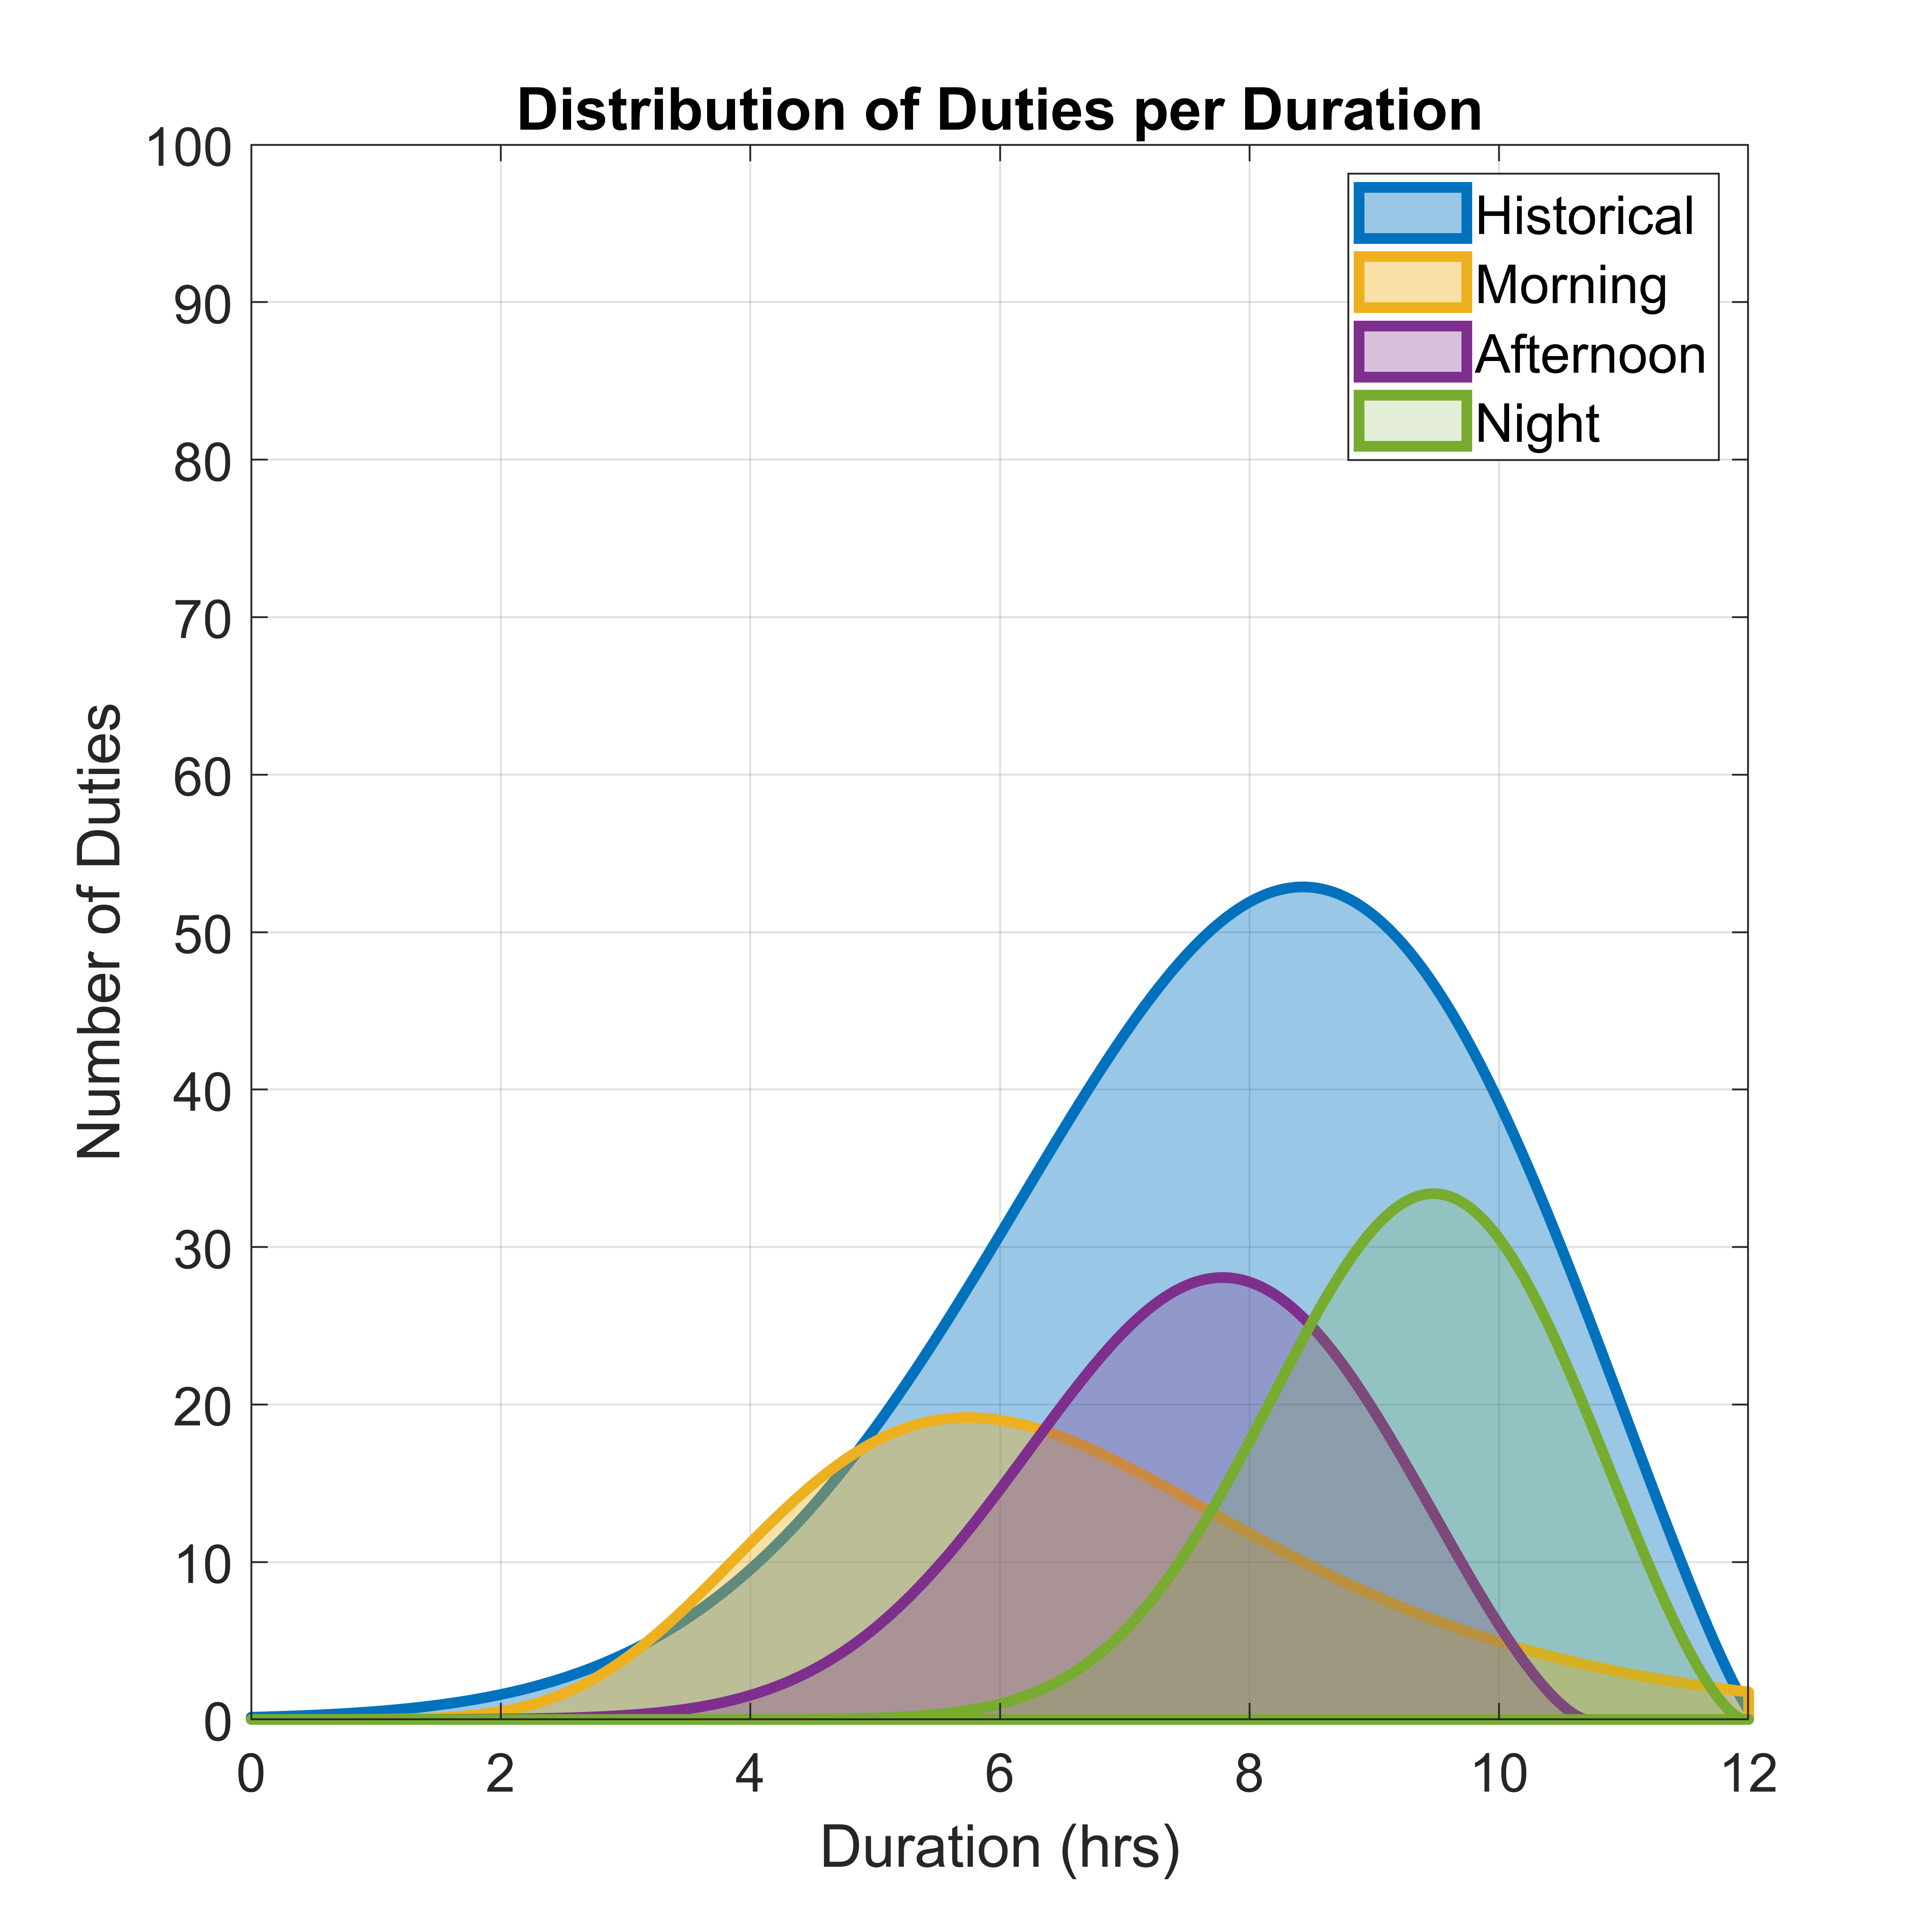
\includegraphics[width=0.46\linewidth]{[1] - chapter/Image Files/Waves-instances.png}
    
\end{center}
   \caption{The effect of splitting the Historical dataset into \textbf{wave instances} of the problem.}
\label{fig: Wave-instances.}
\end{figure}
\vspace*{4in}

\chapter{Mixed-Integer Linear Modelling and Analysis of Historical Schedules}
\label{chapter: 2-Evaluating Royal Mail Historical Data}

%%%%%%%%%%%%%%%%%%%%%%%%%%%%%%%%%%%%%%%%%%%%%%%%%%%%%%%%%%%%%%%%%%%%%%%%%%%%%%% SECTION %%%%%%%%%%%%%%%%%%%%%%%%%%%%%%%%%%%%%%%%%%%%%%%%%%%%%%%%%%%%%%%%%%%%%%%%%%%%%%
This chapter concerns the formulation of an initial set of models used to provide a first assessment on the opportunity for optimisation that is available in our problem. The goal of this analysis is to corroborate the quest of this dissertation to investigate the opportunity for efficiency gains and optimisation of the current practices run by Royal Mail. 

\vspace{\baselineskip}
\noindent
Section \ref{section: 4.1} starts by defining the playing field within which our models will be developed. It also provides an overview of the actual historical practices implemented by Royal Mail building upon the high-level overview seen in Chapter \ref{chapter: Problem Definition}. Sections \ref{section:Makespan Scheduling-content}-\ref{section: Pre-emptive} each involve the study of a different model, and they all follow a similar organisation. They begin by outlining the motivation behind the use of each of the models, and the goal we wish to achieve with each one. They then present the first set of results of this dissertation, outlining the efficiency gains that can be made for the instances of the supplied dataset.
%%%%%%%%%%%%%%%%%%%%%%%%%%%%%%%%%%%%%%%%%%%%%%%%%%%%%%%%%%%%%%%%%%%%%%%%%%%%%%% SECTION %%%%%%%%%%%%%%%%%%%%%%%%%%%%%%%%%%%%%%%%%%%%%%%%%%%%%%%%%%%%%%%%%%%%%%%%%%%%%%

\section{Modelling Environment}
\label{section: 4.1}
To develop this first set of model formulations, we assume that the schedule instances contain \textbf{fixed duties} with a concrete \texttt{start\_time}, and \texttt{end\_time}. Multiple duties are being run in parallel each day. Our goal is to allocate the trips (i.e. atomic blocks) efficiently to those available duties. We assume carte blanche in regards to our flexibility in allocating a block to a duty by neglecting any restrictions as to whether or not we can move a block. We also render our data points agnostic to any semantics associated with each trip\footnote{e.g. the distance between locations or the day on which each shift should occurs} and assume that all blocks are equivalent in their significance, and are merely characterised by their parameters. These abstractions will enable us to determine the maximum room for improvement that exists in efficiently allocating blocks to each duty establishing an upper bound in regards to the degree to which we can aim to optimise.

%%%%%%%%%%%%%%%%%%%%%%%%%%%%%%%%%%%%%%%%%%%%%%%%%%%%%%%%%%%%%%%%%%%%%%%%%%%%%%% sub-SECTION %%%%%%%%%%%%%%%%%%%%%%%%%%%%%%%%%%%%%%%%%%%%%%%%%%%%%%%%%%%%%%%%%%%%%%%%%%%%%%
\vspace{\baselineskip}
\noindent
The set of assumptions mentioned are succinctly summarised below:


%%%%%%%%%%%%%%%%%%%%%%%%%%%%%%%%%%%%%%%%%%%%%%%%%%%%%%%%%%%%%%%%%%%%%%%%%%%%%%% Table %%%%%%%%%%%%%%%%%%%%%%%%%%%%%%%%%%%%%%%%%%%%%%%%%%%%%%%%%%%%%%%%%%%%%%%%%%%%%%

	\begin{table}[ht]
	\renewcommand{\arraystretch}{1.7} %adds space between cells of a table
		\centering
		\begin{tabular}{|c |p{0.9\textwidth}|} 
			\multicolumn{2}{l}{\textbf{Simplifying Assumptions}} \\
		    \hline
			\textbf{(1)}  & The \textbf{duration} of a \textbf{block} stays \textbf{constant}, irrespective of the timing of its occurrence.\\
            \hline
            \textbf{(2)}  & The \texttt{start}, \texttt{end} times and \textbf{durations} of duties remain fixed. \\
            \hline
            \textbf{(3)}  &\textbf{Atomic blocks} are \textbf{freely interchangeable}, within the spectrum of a schedule.\\
			\hline
			\textbf{(4)}  & The \textbf{routes} are \textbf{fixed}, and we \textbf{maintain} the \textbf{order} with which we visit external locations.\\
			\hline
		\end{tabular} 
	\end{table}
	
\vspace{\baselineskip}
\noindent
The first two assumptions, capture the fact that our proposed schedules respect the principle of \textbf{conservation of time}. Our models receive as input an instance that contains blocks inside duties the sum of the durations of which gives us the \texttt{overall labor time} to be scheduled. The schedules that are generated from our algorithms have the same blocks, covering the same \texttt{overall labor time} with the only difference being the \textbf{arrangement}, of those blocks in the duties. The third assumptions, refers to our \textit{assignment policy} of blocks to duties, and the fact that it is completely open-ended giving the schedule total freedom over which duty, and at what point in time to assign a block. Finally, the last assumption reiterates that we do not focus on the routing aspect of this Vehicle-Routing like problem but only study its scheduling portion.
	

	
	%%%%%%%%%%%%%%%%%%%%%%%%%%%%%%%%%%%%%%%%%%%%%%%%%%%%%%%%%%%%%%%%%%%%%%%%%%%%%%% sub-SECTION %%%%%%%%%%%%%%%%%%%%%%%%%%%%%%%%%%%%%%%%%%%%%%%%%%%%%%%%%%%%%%%%%%%%%%%%%%%%%%
	
\subsection*{Evaluation of Historical Schedules}
To begin assessing the performance of our optimised schedule we must first look at the schedules currently run by Royal Mail which we refer to as the \textbf{historical} instance.

%%%%%%%%%%%%%%%%%%%%%%%%%%%%%%%%%%%%%%%%%%%%%%%%%%%%%%%%%%%%%%%%%%%%%% Table %%%%%%%%%%%%%%%%%%%%%%%%%%%%%%%%%%%%%%%%%%%%%%%

\begin{table}[h]
\small
    \centering 
    \begin{tabular}{|c|c|c|c|c|c|c|}
        \hline
        \textbf{Instance} & \multicolumn{3}{|c|}{ \textbf{Characteristics}} & \multicolumn{3}{|c|}{ \textbf{Blocks (HH:mm)}}  \\
        \hline
        & \texttt{Duties} & \texttt{Blocks} & \texttt{Activities} & \texttt{Average} &  \texttt{Minimum} & \texttt{Maximum} \\
        \hline
        Historical & 183 & 462 & 3,285 & 03:05 & 00:40 & 08:25 \\
        \hline
    \end{tabular}%
    \medbreak
\end{table}


\vspace{\baselineskip}
\noindent
The historical schedules which our model is given as an input are driven by an instance $I = \langle{m},B\rangle{}$ of the problem where 462 blocks are allocated among a set of 183 duties over the period of a week\footnote{As input we provide the Finalised Dataset (Cleaned) from Section \ref{section: Data Cleaning} of the previous chapter that we henceforth refer to as the Historical Schedule.}. The minimal processing time $p_{j}$ was that of a round-trip lasting only 40 minutes while the longest trips lasted up to 8 hours and 25 minutes. On average a round-trip is expected to last 3 hours and 5 minutes among the historical schedules. 


%%%%%%%%%%%%%%%%%%%%%%%%%%%%%%%%%%%%%%%%%%%%%%%%%%%%%%%%%%%%%%%%%%%%%% Table %%%%%%%%%%%%%%%%%%%%%%%%%%%%%%%%%%%%%%%%%%%%%%%

\begin{table}[h]
\small
    \centering 
    \begin{tabular}{|c|c|c|c|c|}
        \hline
        \textbf{Schedule} & \multicolumn{3}{|c|}{ \textbf{Duties (HH:mm)}} & \textbf{Total Time (HH:mm)}  \\
        \hline
        & \texttt{Average} &  \texttt{Minimum} & \texttt{Makespan} & \\
        \hline
        Historical & 07:50 & 02:50 & 11:50 & 1,435:22 \\
        \hline
    \end{tabular}%
    \medbreak
\end{table}
\vspace{\baselineskip}
\noindent
We proceeded to plot a histogram of the duty structure of the historical schedule, seen in Figure \ref{fig: Historical for Evaluation.}. In that diagram we have fitted the historical workload into class intervals or histogram bins that represent durations of duties according to the duties of the historical schedule. The purpose of this figure is to show us how much each driver works historically. Indeed, there is a \textbf{noticeable variation}. We see some drivers work for around 2 hours whereas others for close to 12 hours and in general there are some \textbf{significant fluctuations}, which provokes a waste of labour hours. In general, there are people asked to perform duties in excess of 9 hours, hence requiring \textbf{overtimes}, which might prove costly for the company. Hence, envisioning a more balanced schedule we wanted to see if it is possible to have a solution that balances the workload more uniformly. This motivated the experiment run in Section \ref{section:Makespan Scheduling-content}, where since our goal is a balanced schedule we choose a formulation based on the \textit{Makespan Scheduling} model first seen in Section \ref{section:Makespan Scheduling}. The motivation behind this choice is that as was explained in Section \ref{section:Makespan Scheduling}, a schedule with a minimised \textit{makespan} usually achieves a \textbf{well-balanced} sequence of the tasks processed \cite{DUMMY:2}.


%%%%%%%%%%%%%%%%%%%%%%%%%%%%%%%%%%%%%%%%%%%%%%%%%%%%%%%%%%%%%%%%%%%%%%%%%%%%% Figure %%%%%%%%%%%%%%%%%%%%%%%%%%%%%%%%%%%%%%%%%%%%%%%%%%%%%%%%%%%%%%%%%%%%%%%%%%%%%%

\begin{figure}[ht]
\begin{center}
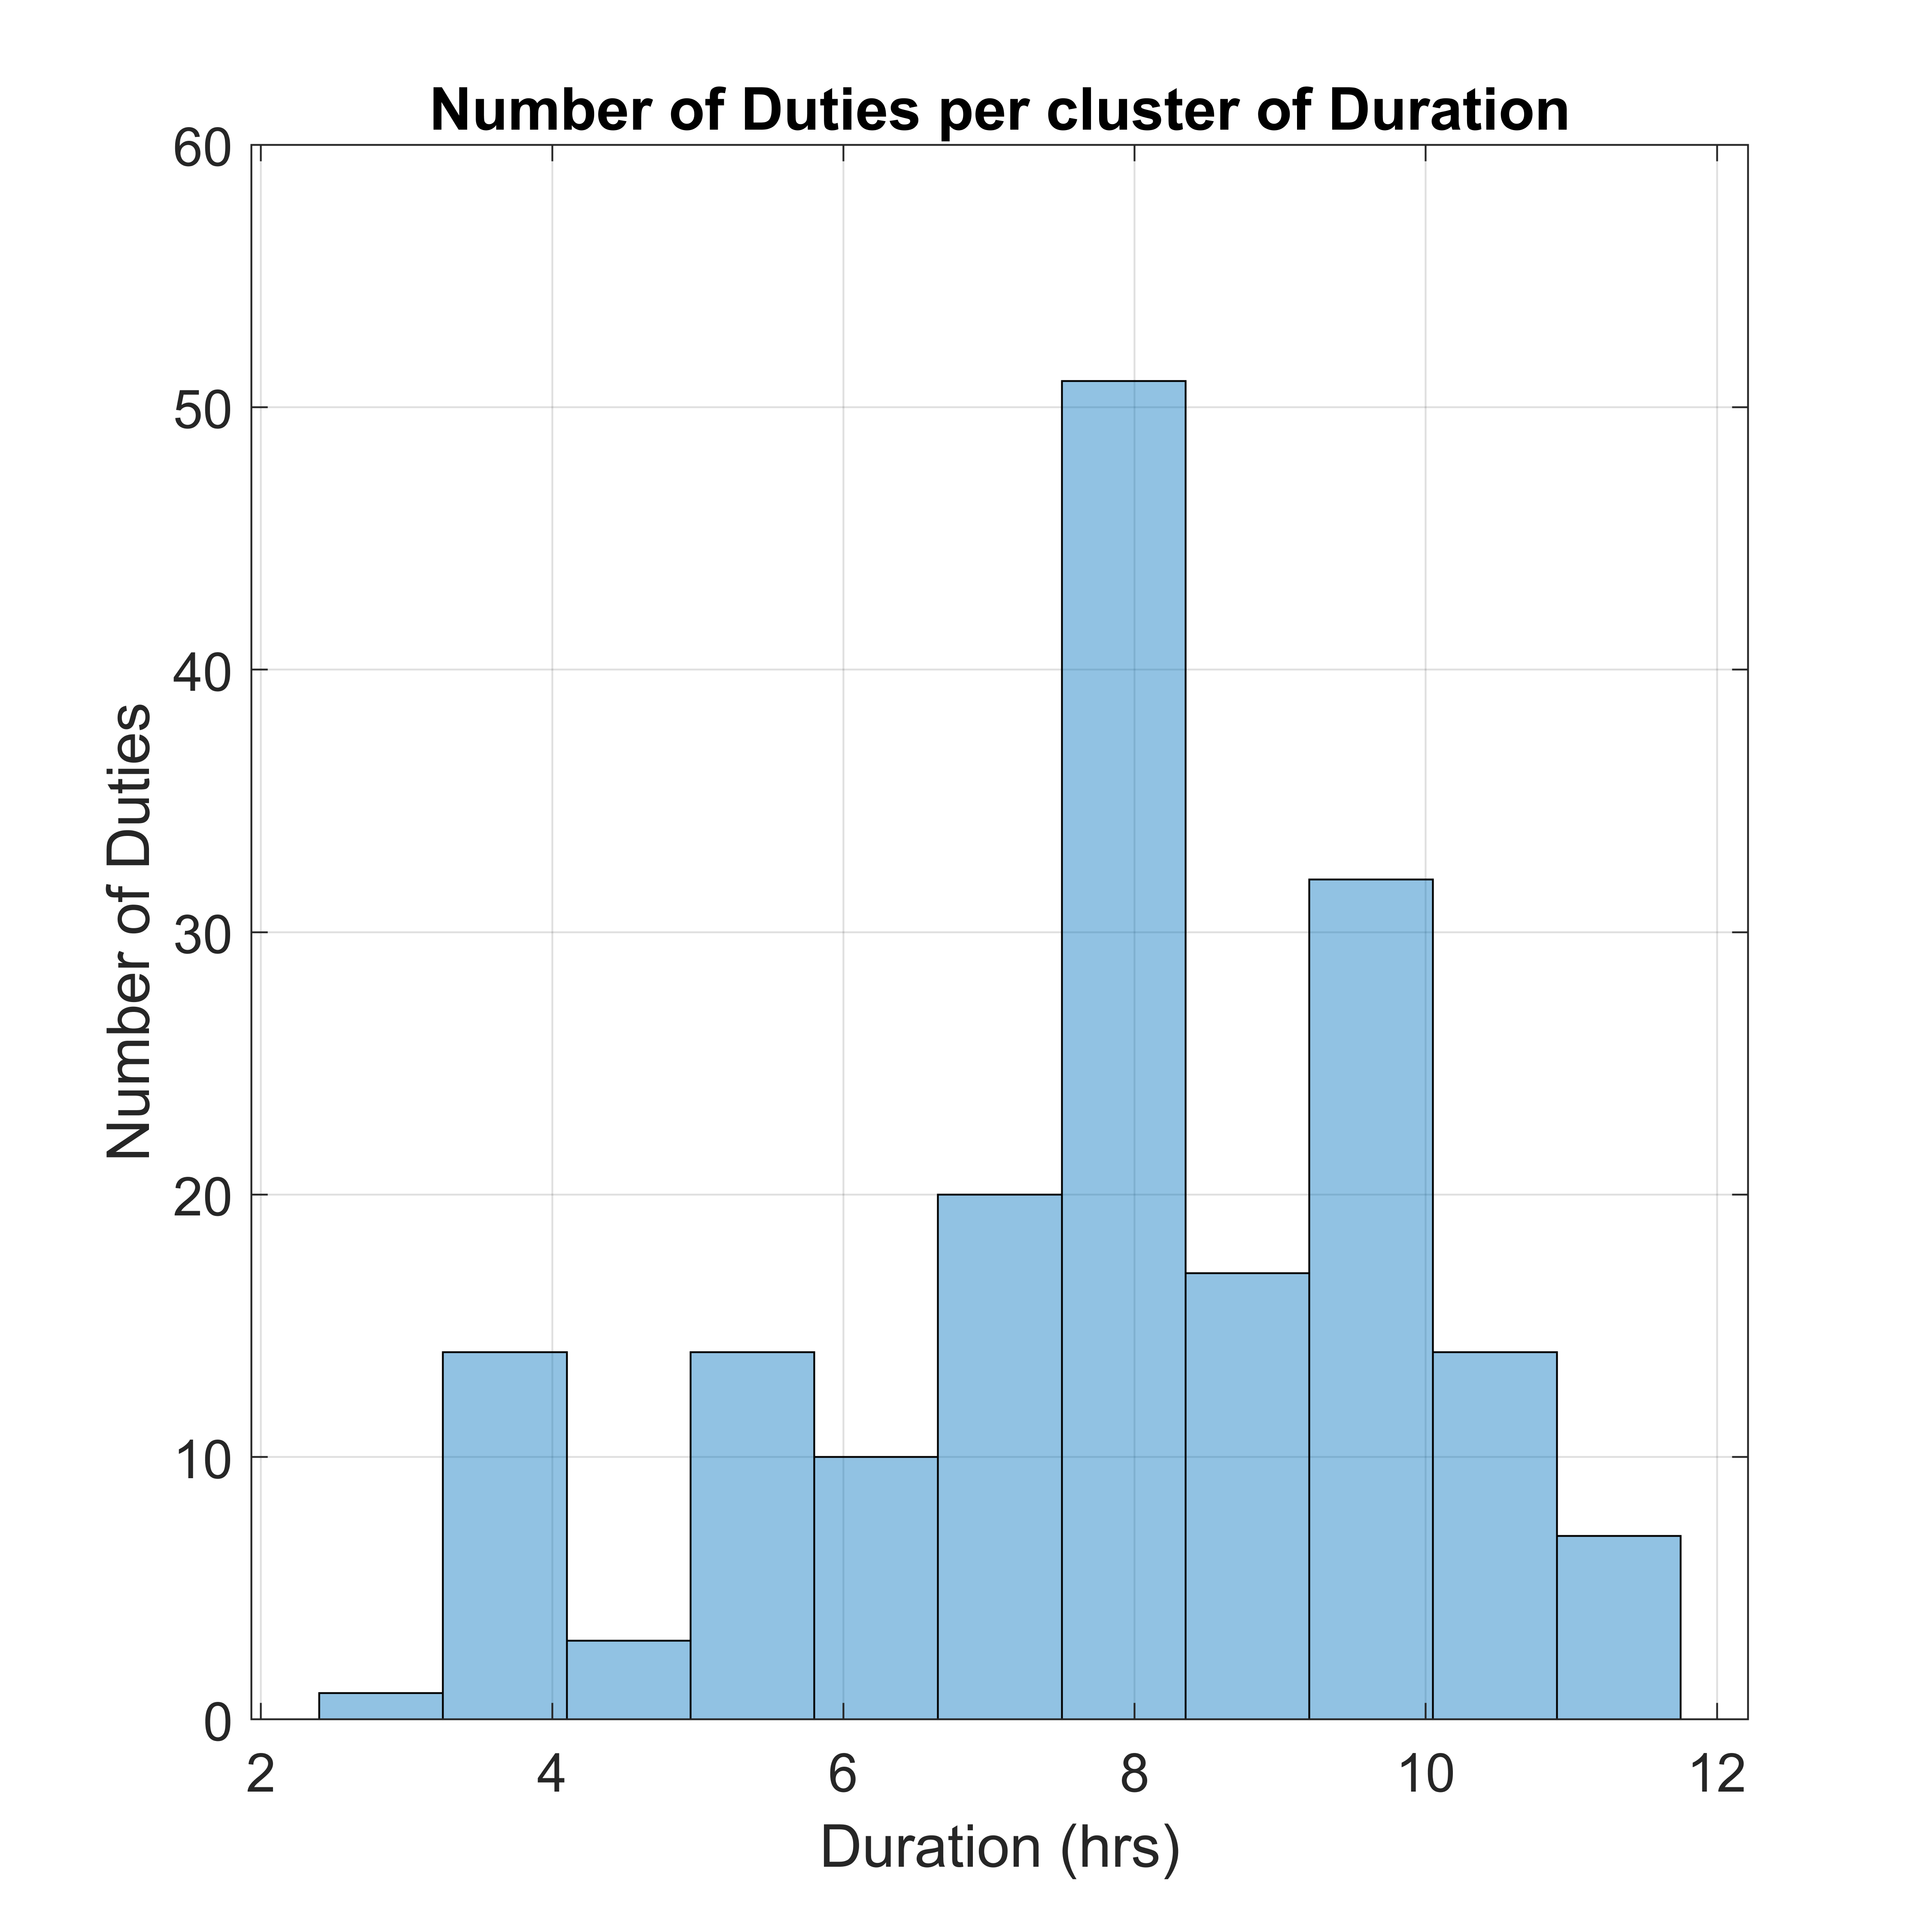
\includegraphics[width=0.46\linewidth]{[1] - chapter/Image Files/Historical-for-evaluation.png}
    
\end{center}
   \caption{The histogram provides an overview of the overall $Duty$ lengths featured in the \textbf{Historical Schedule}.}
\label{fig: Historical for Evaluation.}
\end{figure}

%%%%%%%%%%%%%%%%%%%%%%%%%%%%%%%%%%%%%%%%%%%%%%%%%%%%%%%%%%%%%%%%%%%%%%%%%%%%%%% SUBSECTION %%%%%%%%%%%%%%%%%%%%%%%%%%%%%%%%%%%%%%%%%%%%%%%%%%%%%%%%%%%%%%%%%%%%%%%%%%%%%%

\section{Load Balancing}
\label{section:Makespan Scheduling-content}
With the goal of finding a more balanced schedule in terms of duty length the \textit{Makespan Scheduling} formulation attempts to minimise the overall duration of the schedule, the \textbf{makespan}. The goal is for the resulting optimised schedule to decrease the amount of time for which a driver is generally occupied for, a practical advantage that we hope will be gained by a \textbf{balanced schedule}.

\vspace{\baselineskip}
\noindent
The two evaluation criteria that we need to examine to determine the success of our model are the degree to which the \textit{makespan is decreased} and a \textit{measure of uniformity} of the optimised schedule. Two ways to practically evaluate these two criteria is to look at the \textbf{(\%) makespan reduction} and the \textbf{(\%) standard deviation reduction ($\pmb{\sigma}$)} of the distribution of duties, respectively, compared to the instance that was provided as input to the model. Hence, for the experiments involving the Makespan model, we compare every schedule generated at each stage with respect to those two measures of success. 

\vspace{\baselineskip}
\noindent
An instance $I = \langle{m},B\rangle{}$ of the problem involves  an environment of $D=\{1,...,m\}$ parallel and identical duties, and a set of blocks $B =\{1,...,n\}$. Each duty may be assigned at most \textbf{one block per unit of time}, and once assigned a block it must execute it until its completion with no interruptions. In other words, this is a \textit{non-preemptive} model. %A duty is described by its start time $s_{i}$, and finish time $f_{i}$. The execution of any blocks for each duty must occur within the time horizon $f_{i}-s_{i}$. 
The blocks $j \in B$ are all associated with processing time $p_{j}$ as their one and only attribute. Mathematically the goal for this first stage of optimisation is to evenly allocate the blocks to each duty in a way that minimises the completion time of the last duty to be completed. 

\vspace{\baselineskip}
\noindent
The formulation utilised to perform this task is an adapted version %aka a variance
of the makespan scheduling model seen in Chapter \ref{chapter: Background}. We parallelise\footnote{The purpose of this parallelisation is to transform our problem into an equivalent problem to that studied in \cite{PRAKASH2010}, for which efficient algorithms for solving it have already been studied.} our problem with the problem observed in Section \ref{section:Makespan Scheduling}. We consider a \textbf{duty} as the \textit{machine} from formulation \ref{section:Makespan Scheduling} and a \textbf{block} as a \textit{job}, respectively. Hence, our formulation assigns blocks to duties. Binary variable $x_{i,j}$ dictates the assignment of a block $j$ to a duty $i$. The binary variable $x_{i,j}$ is equal to 1 if the atomic block $j \in B$ is assigned to duty $i \in D$, and 0 otherwise. Continuous variable $y$ contains the \textbf{makespan} of the schedule, which is what we are trying to minimise.  

%%%%%%%%%%%%%%%%%%%%%%%%%%%%%%%%%%%%%%%%%%%%%%%%%%%%%%%%%%%%%%%%%%%%%%%%%%%%%%% Maths %%%%%%%%%%%%%%%%%%%%%%%%%%%%%%%%%%%%%%%%%%%%%%%%%%%%%%%%%%%%%%%%%%%%%%%%%%%%%%

\vspace{\baselineskip}
\begin{equation}
\label{equation: Makespan Scheduling}
\begin{aligned}
&\text{minimise}
%& & y_{i}  \\ %\todo{why y and and not yi}
& & y  \\ 
& \text{subject to}
% & & y_{i} = \sum _{j=1}^n x_{i,j}p_{j}  \;\;\; &\forall \; i \in D\tag{1}\\   
& & y \geq \sum _{j=1}^n x_{i,j}p_{j}  \;\;\; &\forall \; i \in D\\   
& & &\sum _{i=1}^m x_{i,j} = 1 \;\;\; &\forall \; j \in B\\
% & & &\sum _{j=1}^n x_{i,j}p_{j} \leq f_{i}-s_{i} \;\;\; &\forall \; i \in D\\ %{\color{red} we deleted the constraint that involves the length of duty being less than end-start.}
& & & y\geq 0  \\
& & & x_{i,j} \in  \{ 0,1 \} \;\;\; &\forall \; j \in B, \; i \in D\\
\end{aligned}
\end{equation}

\vspace{\baselineskip}
\noindent
The objective is to get the \textbf{minimal} possible \textbf{makespan} that allows a feasible schedule. The first constraint assigns $y$ its definition of the \textbf{makespan} by making it equal to the completion time of the last atomic block to be executed. With the second constraint we make sure that each block is assigned to at least one but only one duty. The third and the fourth constraints enforce the continuous and integrality nature to the $y,x$ variables respectively, rendering this a \textit{MILP} problem.

%%%%%%%%%%%%%%%%%%%%%%%%%%%%%%%%%%%%%%%%%%%%%%%%%%%%%%%%%%%%%%%%%%%%%%%%%%%%%%% sub-SECTION %%%%%%%%%%%%%%%%%%%%%%%%%%%%%%%%%%%%%%%%%%%%%%%%%%%%%%%%%%%%%%%%%%%%%%%%%%%%%%

\subsection*{Evaluation}
In this initial model, we choose to focus on trying to shorten the \textbf{completion time} of the \textbf{longer lasting duty}, with the goal of obtaining \textbf{fairer shifts }that will have a more \textbf{uniform} allocation of the workload among drivers. In the historical schedule, the shortest shift lasts for 2 hours and 50 minutes while the longest one (i.e. the makespan) takes 11 hours and 50 minutes, as seen before. The historical allocation of blocks has been done heuristically, for the historical schedules, which is why cases of longer and shorter shifts than the average tend to occur. Taking as an example, the extremely short and long cases of shifts described above a closer observation shows that more than seven blocks (i.e. round-trips) were allocated to a driver as part of that longest shift, whereas just a single one was assigned to the shortest shift. Such observations motivate our efforts in striving to improve efficiency by minimising the duration of every duty to ensure a fairer allocation of the work load, since there seems to be a chance to remedy all these oddities of the historical schedule.

\vspace{\baselineskip}
\noindent
With regards to the objective of our model, the makespan, we need to be aware of a practical constraint that places a lower bound regarding the most minimum makespan that can be achieved in a feasible schedule. This constraint stems from the fact the there exist blocks of duration 8 hours and 25 minutes. According to assumption (4) of Section \ref{section: 4.1}, we cannot split a block into smaller sub-components so as to reduce its duration. Consequently, the \texttt{absolute theoretical limit} in regards to the most optimal schedule that we can hope to achieve will have a makespan equal to the duration of those maximum-lasting blocks. Such a schedule would contain duties that solely complete these 08:25 block and no other. Proposing a schedule with an 08:25 makespan or one close to it will constitute an efficient optimisation of the current practices. 

%%%%%%%%%%%%%%%%%%%%%%%%%%%%%%%%%%%%%%%%%%%%%%%%%%%%%%%%%%%%%%%%%%%%%%%%%%%%%%% Figure %%%%%%%%%%%%%%%%%%%%%%%%%%%%%%%%%%%%%%%%%%%%%%%%%%%%%%%%%%%%%%%%%%%%%%%%%%%%%%

\begin{figure}%
    \centering
    \subfloat[The duration of each duty before and after optimisation sorted in increasing duration.]{%\begin{center}
    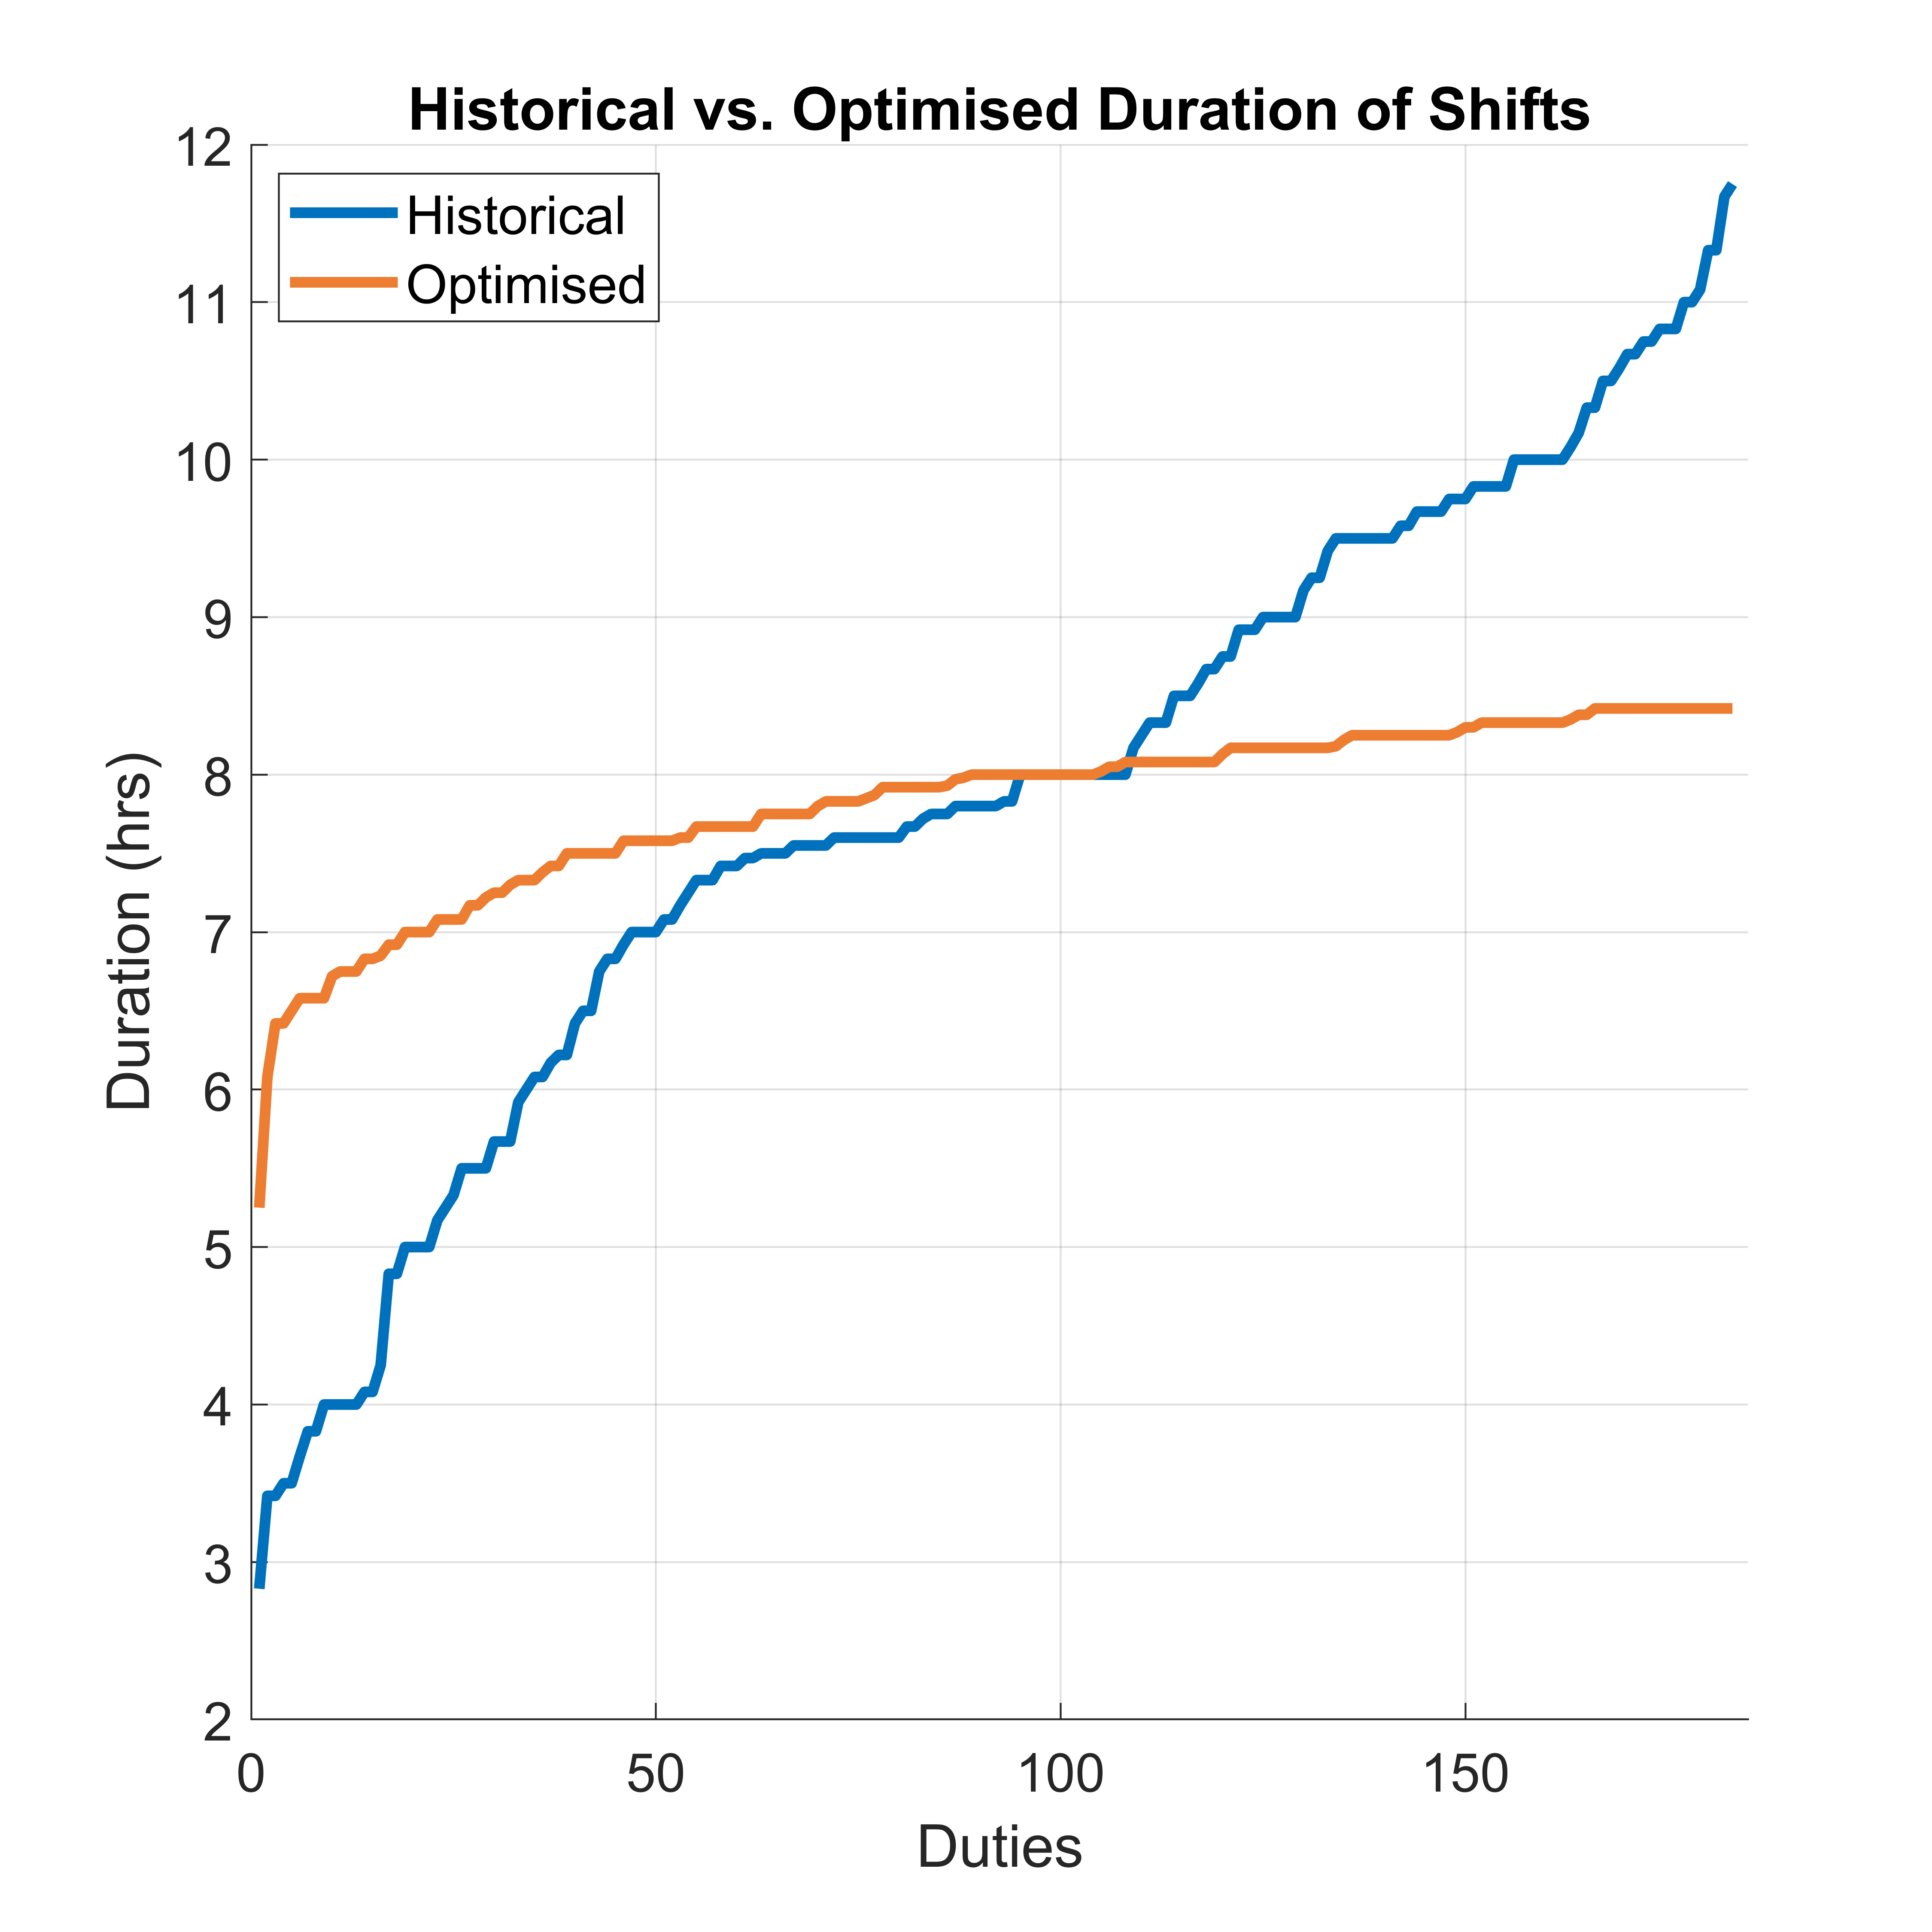
\includegraphics[width=0.46\linewidth]{[1] - chapter/Image Files/1-D1.png}
    }%\end{center}}%picture #1
    \qquad
    %picture #2
    \centering
    \subfloat[Histogram showing the improvement in the \textbf{uniformity} of duties.]{%\begin{center}
    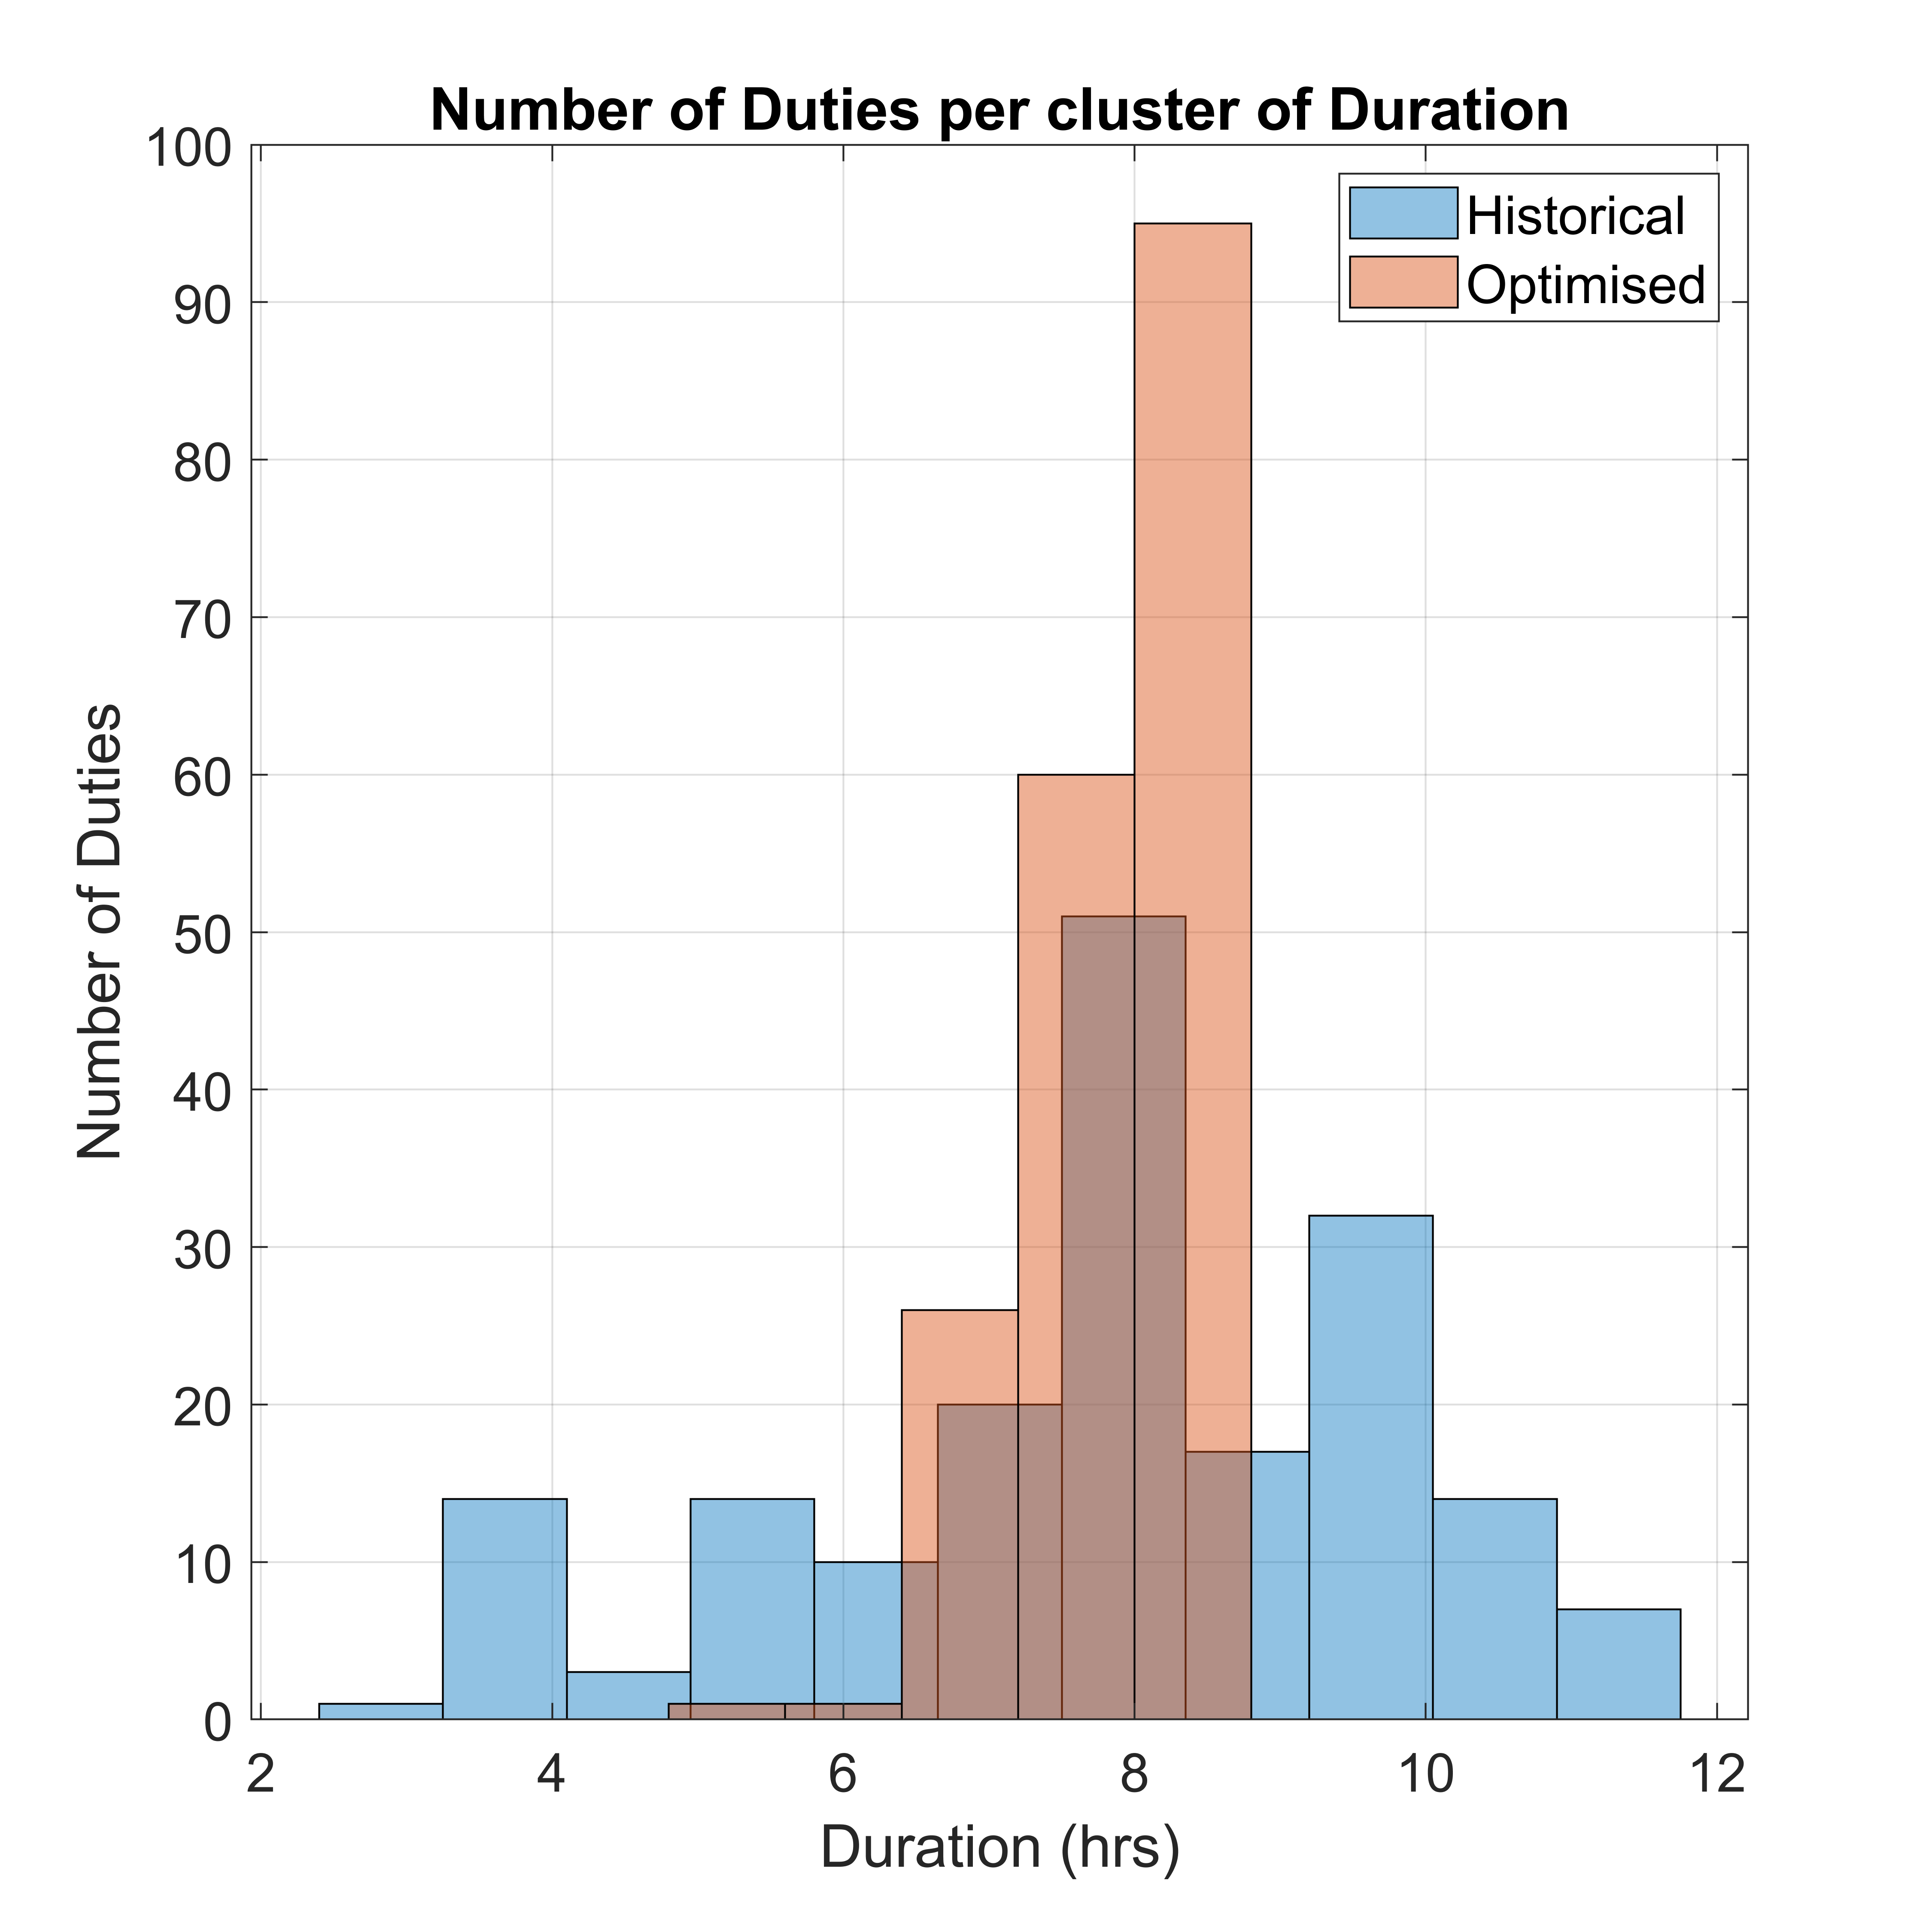
\includegraphics[width=0.46\linewidth]{[1] - chapter/Image Files/1-D1M1.png}
    }%\end{center}}%end of picture #2
    \caption{Figures illustrating the effects of the optimisation model on the historical duties.}%
    \label{fig:1-D1M1}%
\end{figure}

%%%%%%%%%%%%%%%%%%%%%%%%%%%%%%%%%%%%%%%%%%%%%%%%%%%%%%%%%%%%%%%%%%%%%%%%%%%%%%% sub-SECTION %%%%%%%%%%%%%%%%%%%%%%%%%%%%%%%%%%%%%%%%%%%%%%%%%%%%%%%%%%%%%%%%%%%%%%%%%%%%%%

\subsubsection*{Qualitative Results}
The application of the Makespan Scheduling model on the Historical dataset has the effect of \textit{flattening} the historical curve as seen in Figure \ref{fig:1-D1M1}(a), and hence concentrating the majority of the workload on duties that last as long as the makespan of the schedule, or less. 

\vspace{\baselineskip}
\noindent
The effect of our model is most noticeable in Figure \ref{fig:1-D1M1}(b) which plots the duration of each duty before and after the optimisation. We can observe how this first attempt at optimising the historical schedule results in a fairer distribution of labor time, since the majority of duties are now of similar length. There is also a big improvement in the \textbf{reduction of extremities} vis-\`a-vis extremely long and extremely short shifts, allowing us to prevent the occurrence of a large group of very long duties that are not efficient since they require drivers to complete overtimes. In a nutshell a reduction of the order of \textbf{72\%} in the \textbf{standard deviation ($\pmb{\sigma}$)} of the optimised schedule compared to the input instance encapsulates the fact that we have achieved our main goal of obtaining a more uniform schedule.

\subsubsection*{Quantitative Results}

%%%%%%%%%%%%%%%%%%%%%%%%%%%%%%%%%%%%%%%%%%%%%%%%%%%%%%%%%%%%%%%%%%%%%% Table %%%%%%%%%%%%%%%%%%%%%%%%%%%%%%%%%%%%%%%%%%%%%%%

\begin{table}[h]
\small
    \centering 
    \begin{tabular}{|l|c|c|c|c|}
        \hline
        \textbf{Schedule} & \multicolumn{3}{|c|}{ \textbf{Duties (HH:mm)}} & \textbf{Total Time (HH:mm)}  \\
        \hline
        & \texttt{Average} &  \texttt{Minimum} & \texttt{Makespan} & \\
        \hline
        Historical & 07:50 & 02:50 & 11:50 & 1,435:22 \\
        \hline
        Historical\_Optimised & 07:50 & 05:15 & 08:25 & 1,435:22 \\
        \hline
    \end{tabular}%
    \medbreak
\end{table}


\vspace{\baselineskip}
\noindent
We have also achieved our main objective of minimising the \textit{maximum duty length} since the historical makespan was 11 hours and 45 minutes whereas in our revised schedule it is exactly 8 hours and 25 minutes hence, achieving the \texttt{absolute theoretical limit}. This accomplishment amounts to a \textbf{28\% reduction of the makespan} compared to the historical instance received as input. In essence, we have redistributed the load\footnote{The principle of \textbf{conservation of time} is respected as observed on the \texttt{Average} and Total Time columns of the table.} so that some people will not need to be working \textbf{overtimes} hence resulting in efficiency cost cuts for Royal Mail. A side-effect of our scheduling is that some drivers will be working a bit more. As far as Royal Mail is concerned this is a welcome change since it means we will be utilising the drivers' time better.

\vspace{\baselineskip}
\noindent
It is evident in the historical schedule in Figure \ref{fig:1-D1M1}(b) that duties lasting between 8-11.7 hours take a larger load of the work while the rest of the shifts carry out a smaller portion of the overall workload. By making an effort to redistribute the load in a more uniform fashion we are able to achieve a \textbf{fairer allocation} of the amount of work required by assigning the load of the long lasting shift to the frequently occurring shifts of up to 8 hours and 25 minutes. We distributed the load from the previously shorter and longer lasting shifts to those frequently occurring ones. The outcome, was an increase in the duration of the shorter lasting shifts resulting in a fairer allocation of the load. However, this also resulted in an increase in the frequency with which the around 8 hour lasting shifts occur. This is an unwanted side-effect of this redistribution of load since even though we reduce the toll taken by the most frequently occurring shift, we distribute a portion of it on the longer-lasting shifts which are already overwhelmed. 

\vspace{\baselineskip}
\noindent
A synopsis of the statistics that highlight the performance of our model for the Historical schedule as the input instance is found below:
%%%%%%%%%%%%%%%%%%%%%%%%%%%%%%%%%%%%%%%%%%%%%%%%%%%%%%%%%%%%%%%%%%%%%% Table %%%%%%%%%%%%%%%%%%%%%%%%%%%%%%%%%%%%%%%%%%%%%%%

\begin{table}[h]
\small
    \centering 
\begin{tabular}{c|c|c}
        \textbf{Schedule} & \textbf{Makespan Reduction (\%)} & \textbf{Maximum Difference-Reduction \cite{maxdif} (\%)} \\
        \hline
         Historical\_Optimised & 28\% & 72\% \\
\end{tabular}
\end{table}

%%%%%%%%%%%%%%%%%%%%%%%%%%%%%%%%%%%%%%%%%%%%%%%%%%%%%%%%%%%%%%%%%%%%%%%%%%%%%%% sub-SECTION %%%%%%%%%%%%%%%%%%%%%%%%%%%%%%%%%%%%%%%%%%%%%%%%%%%%%%%%%%%%%%%%%%%%%%%%%%%%%%



%%%%%%%%%%%%%%%%%%%%%%%%%%%%%%%%%%%%%%%%%%%%%%%%%%%%%%%%%%%%%%%%%%%%%%%%%%%%%%% sub-SECTION %%%%%%%%%%%%%%%%%%%%%%%%%%%%%%%%%%%%%%%%%%%%%%%%%%%%%%%%%%%%%%%%%%%%%%%%%%%%%%

\subsection*{Evaluation - Optimising Redefined Instance}

%%%%%%%%%%%%%%%%%%%%%%%%%%%%%%%%%%%%%%%%%%%%%%%%%%%%%%%%%%%%%%%%%%%%%% Table %%%%%%%%%%%%%%%%%%%%%%%%%%%%%%%%%%%%%%%%%%%%%%%

\begin{table}[h]
\small
    \centering 
    \begin{tabular}{|c|c|c|c|c|c|c|}
        \hline
        \textbf{Instance} & \multicolumn{3}{|c|}{ \textbf{Characteristics}} & \multicolumn{3}{|c|}{ \textbf{Blocks (HH:mm)}}  \\
        \hline
        & \texttt{Duties} & \texttt{Blocks} & \texttt{Activities} & \texttt{Average} &  \texttt{Minimum} & \texttt{Maximum} \\
        \hline
        Historical & 183 & 462 & 3,285 & 03:05 & 00:40 & 08:25 \\
        \hline
        Redefined & 183 & 462 & 2,850 & 02:25 & 00:30 & 06:35 \\
        \hline
    \end{tabular}%
    \medbreak
\end{table}

\vspace{\baselineskip}
\noindent
We now apply model (\ref{equation: Makespan Scheduling}) to an instance of the Redefined\footnote{Introduced in Section \ref{section: Redefined Dataset} of the previous chapter.} blocks and compare the model's performance with the optimal schedule, previously generated. As mentioned in Section \ref{section: Redefined Dataset}, the Redefined instance is expected to lead us to a better solution, with respect to makespan, since it contains \textbf{less activities} and consequently \textbf{less labour hours to be scheduled}, due the deletion of the non-useful activities. 

%%%%%%%%%%%%%%%%%%%%%%%%%%%%%%%%%%%%%%%%%%%%%%%%%%%%%%%%%%%%%%%%%%%%%%%%%%%%%%% Figure %%%%%%%%%%%%%%%%%%%%%%%%%%%%%%%%%%%%%%%%%%%%%%%%%%%%%%%%%%%%%%%%%%%%%%%%%%%%%%

\begin{figure}%
    \centering
    \subfloat[The duration of each duty before and after optimisation sorted in increasing duration.]{%\begin{center}
    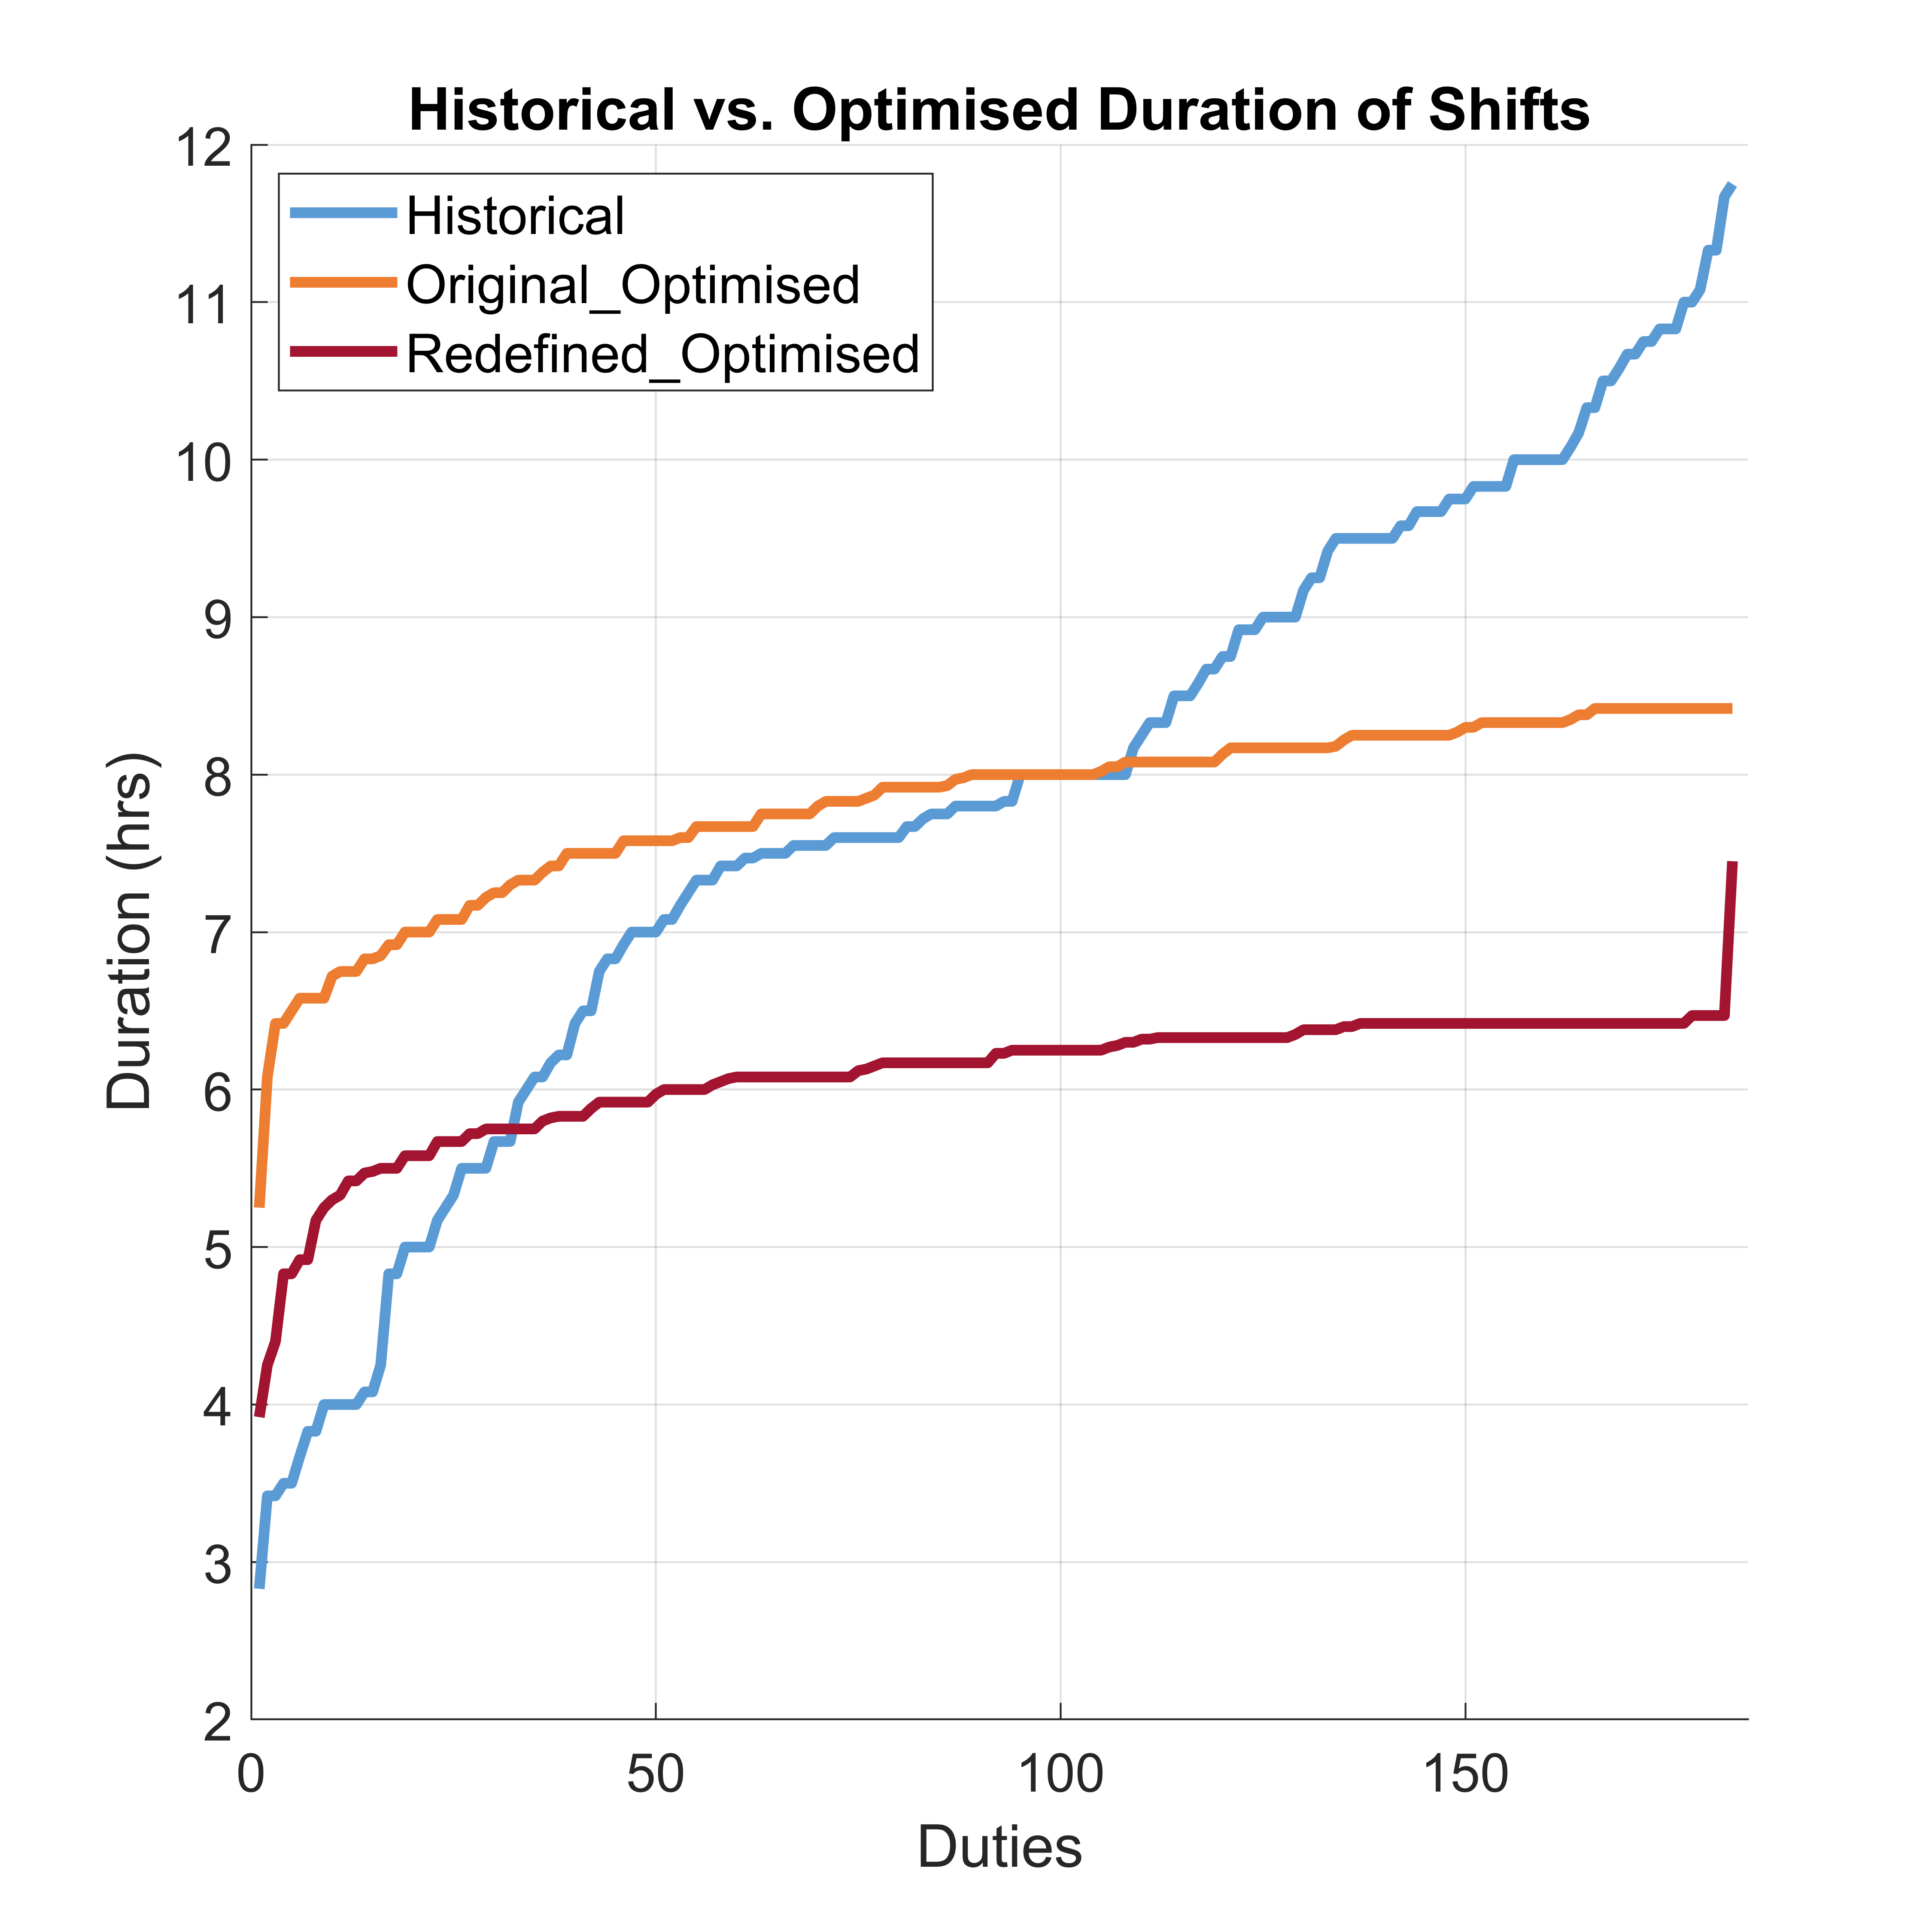
\includegraphics[width=0.46\linewidth]{[1] - chapter/Image Files/1-D2.png}
    }%\end{center}}%picture #1
    \qquad
    %picture #2
    \centering
    \subfloat[Histogram showing the improvement in the uniformity of duties.]{%\begin{center}
    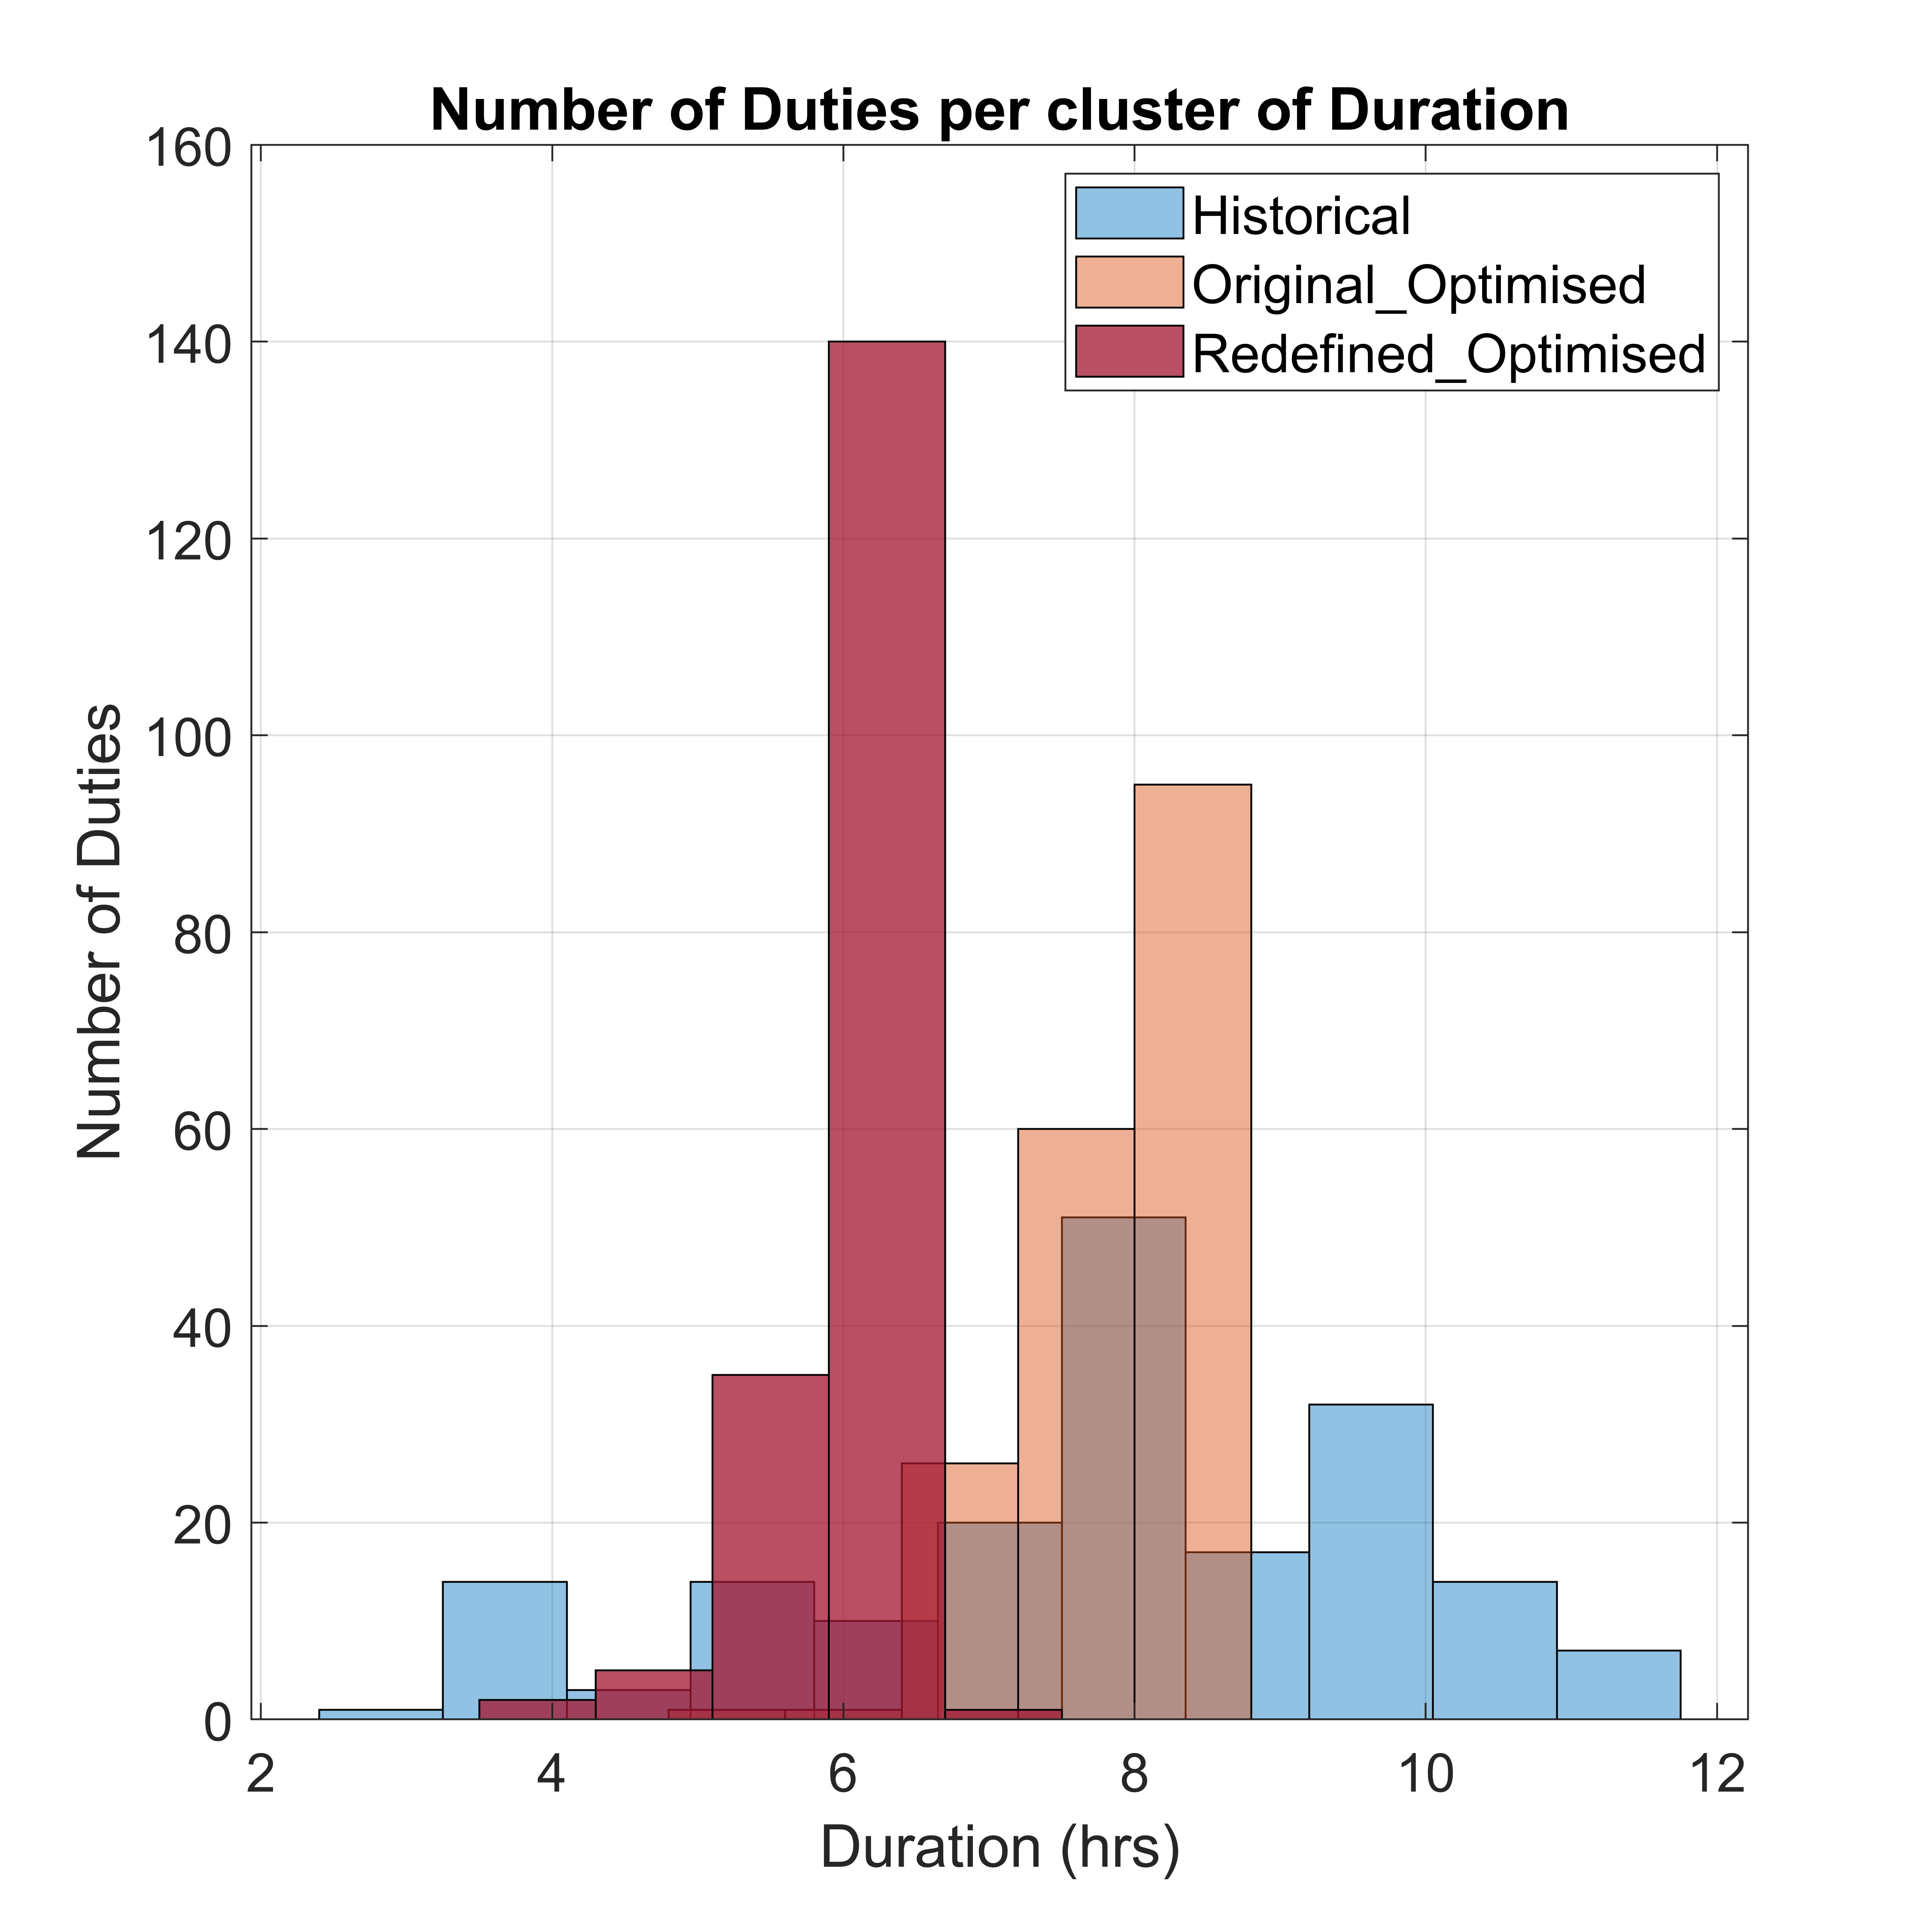
\includegraphics[width=0.46\linewidth]{[1] - chapter/Image Files/1-D2M1.png}
    }%\end{center}}%end of picture #2
    \caption{Illustrations of curves indicating our results.}%
    \label{fig:1-D2M1}%
\end{figure}
 
 %%%%%%%%%%%%%%%%%%%%%%%%%%%%%%%%%%%%%%%%%%%%%%%%%%%%%%%%%%%%%%%%%%%%%% Table %%%%%%%%%%%%%%%%%%%%%%%%%%%%%%%%%%%%%%%%%%%%%%%

\begin{table}[h]
\small
    \centering 
    \begin{tabular}{|l|c|c|c|c|}
        \hline
        \textbf{Schedule} & \multicolumn{3}{|c|}{ \textbf{Duties (HH:mm)}} & \textbf{Total Time}  \\
        \hline
         & \texttt{Average} &  \texttt{Minimum} & \texttt{Makespan} & \\
        \hline
        Historical  & 07:50 & 02:50 & 11:50 & 1,435:22 \\
        \hline
        Historical\_Optimised   & 07:50 & 05:15 & 08:25 & 1,435:22 \\
        \hline
        Redefined\_Optimised   & 06:06 & 03:55 & 07:27 & 1,118:58 \\
        \hline
    \end{tabular}%
    \medbreak
\end{table}
 
\vspace{\baselineskip}
\noindent
Observing the Histogram chart in Figure \ref{fig:1-D2M1}(b), we can see that long lasting shifts have been reduced down to duty lengths which are at the very least, smaller than 7 hours and 27 minutes which is the longest lasting shift (i.e. makespan). The majority of the workload has been assigned to such shifts lasting longer than 6 hours but also generally below the 7 hour mark. With respect to the makespan we see a \textbf{36\% reduction} compared to the historical instance.

\vspace{\baselineskip}
\noindent
The duty that pushes the makespan up to the 07:27 mark occurs only once, and the reason behind its increased duration relative to the bulk of shorter-lasting duties is because it holds the longest lasting block of 6 hours and 35 minutes. As a result, we could argue that the effective makespan of the Redefined schedule is slightly lower in reality since the majority of the duties last approximately 6 and a half hours. Hence, practically the whole cohort of drivers would have to work for 6 and a half hours, except for a single driver that would have to perform the 7 hours and 27 minutes lasting duty.

\vspace{\baselineskip}
\noindent
In terms of encapsulating the performance of generated schedule in a more concrete manner we list the following table outlining how the optimised schedule fairs against our two evaluation criteria:

%%%%%%%%%%%%%%%%%%%%%%%%%%%%%%%%%%%%%%%%%%%%%%%%%%%%%%%%%%%%%%%%%%%%%% Table %%%%%%%%%%%%%%%%%%%%%%%%%%%%%%%%%%%%%%%%%%%%%%%

\begin{table}[h]
\small
    \centering 
\begin{tabular}{c|c|c}
        \textbf{Schedule} & \textbf{Makespan Reduction (\%)} & \textbf{Maximum Difference-Reduction (\%)} \\
        \hline
         Historical\_Optimised & 28\% & 72\% \\
        \hline
         Redefined\_Optimised  & 36\% & 78\% \\ 
\end{tabular}
\end{table}

\vspace{\baselineskip}
\noindent
Comparing the optimised schedules that are created from the Historical and Redefined Instances respectively we see that as expected there is a further reduction of 8\% in the makespan of the Redefined schedule, and also the Redefined schedule has a 6\% lower standard deviation, capturing the fact that it is even more uniform than the Historical schedule. 

%%%%%%%%%%%%%%%%%%%%%%%%%%%%%%%%%%%%%%%%%%%%%%%%%%%%%%%%%%%%%%%%%%%%%%%%%%%%%%% sub-SECTION %%%%%%%%%%%%%%%%%%%%%%%%%%%%%%%%%%%%%%%%%%%%%%%%%%%%%%%%%%%%%%%%%%%%%%%%%%%%%%

\subsection*{Evaluation - Optimising Departure Wave Instances}
As a final experiment on the Makespan Scheduling model we break our problem into separate instances that are designed to resemble the observation made through analysing the dataset\footnote{The \texttt{starting-time} analysis of the dataset mentioned is presented in detail in Appendix \ref{subsection: Appendix Starting times} for interested readers.} concerning the fact that duties tend to start in \textbf{wave}-like clusters. This observation is an important, design parameter that needs to be taken into serious consideration, as it automatically renders any results that we are able to obtain more \textit{practically oriented} and easier to realise from the perspective of Royal Mail. As outlined in Section \ref{section: Wave Instances - Data} we split our dataset into three autonomous sub-problems and we once more run the Makespan Scheduling model.

%%%%%%%%%%%%%%%%%%%%%%%%%%%%%%%%%%%%%%%%%%%%%%%%%%%%%%%%%%%%%%%%%%%%%% Table %%%%%%%%%%%%%%%%%%%%%%%%%%%%%%%%%%%%%%%%%%%%%%%

\begin{table}[h]
\small
    \centering 
    \begin{tabular}{|l|c|c|c|c|c|c|c|}
        \hline
        \textbf{Schedule} & \multicolumn{2}{|c|}{ \textbf{Characteristics}} & \multicolumn{3}{|c|}{ \textbf{Duties (HH:mm)}} & \textbf{Total Time}  \\
        \hline
        & \texttt{Duties} & \texttt{Blocks} & \texttt{Average} &  \texttt{Minimum} & \texttt{Makespan} & \\
        \hline
        Historical\_Optimised & 183 & 462  & 07:50 & 05:15 & 08:25 & 1,435:22 \\
        \hline
        Morning\_Optimised & 59 & 114 & 06:46 & 00:00 & 08:25 & 393:40 \\
        \hline
        Afternoon\_Optimised & 61 & 145 & 07:32 & 03:25 & 07:19 & 444:53 \\
        \hline
        Night\_Optimised & 63 & 203 & 09:27 & 08:40 & 09:30 & 596:34 \\
        \hline
    \end{tabular}%
    \medbreak
\end{table}

%%%%%%%%%%%%%%%%%%%%%%%%%%%%%%%%%%%%%%%%%%%%%%%%%%%%%%%%%%%%%%%%%%%%%%%%%%%%%%% Figure %%%%%%%%%%%%%%%%%%%%%%%%%%%%%%%%%%%%%%%%%%%%%%%%%%%%%%%%%%%%%%%%%%%%%%%%%%%%%%

\begin{figure}
\minipage{0.32\textwidth}
\subfloat[Morning]{%\begin{center}
  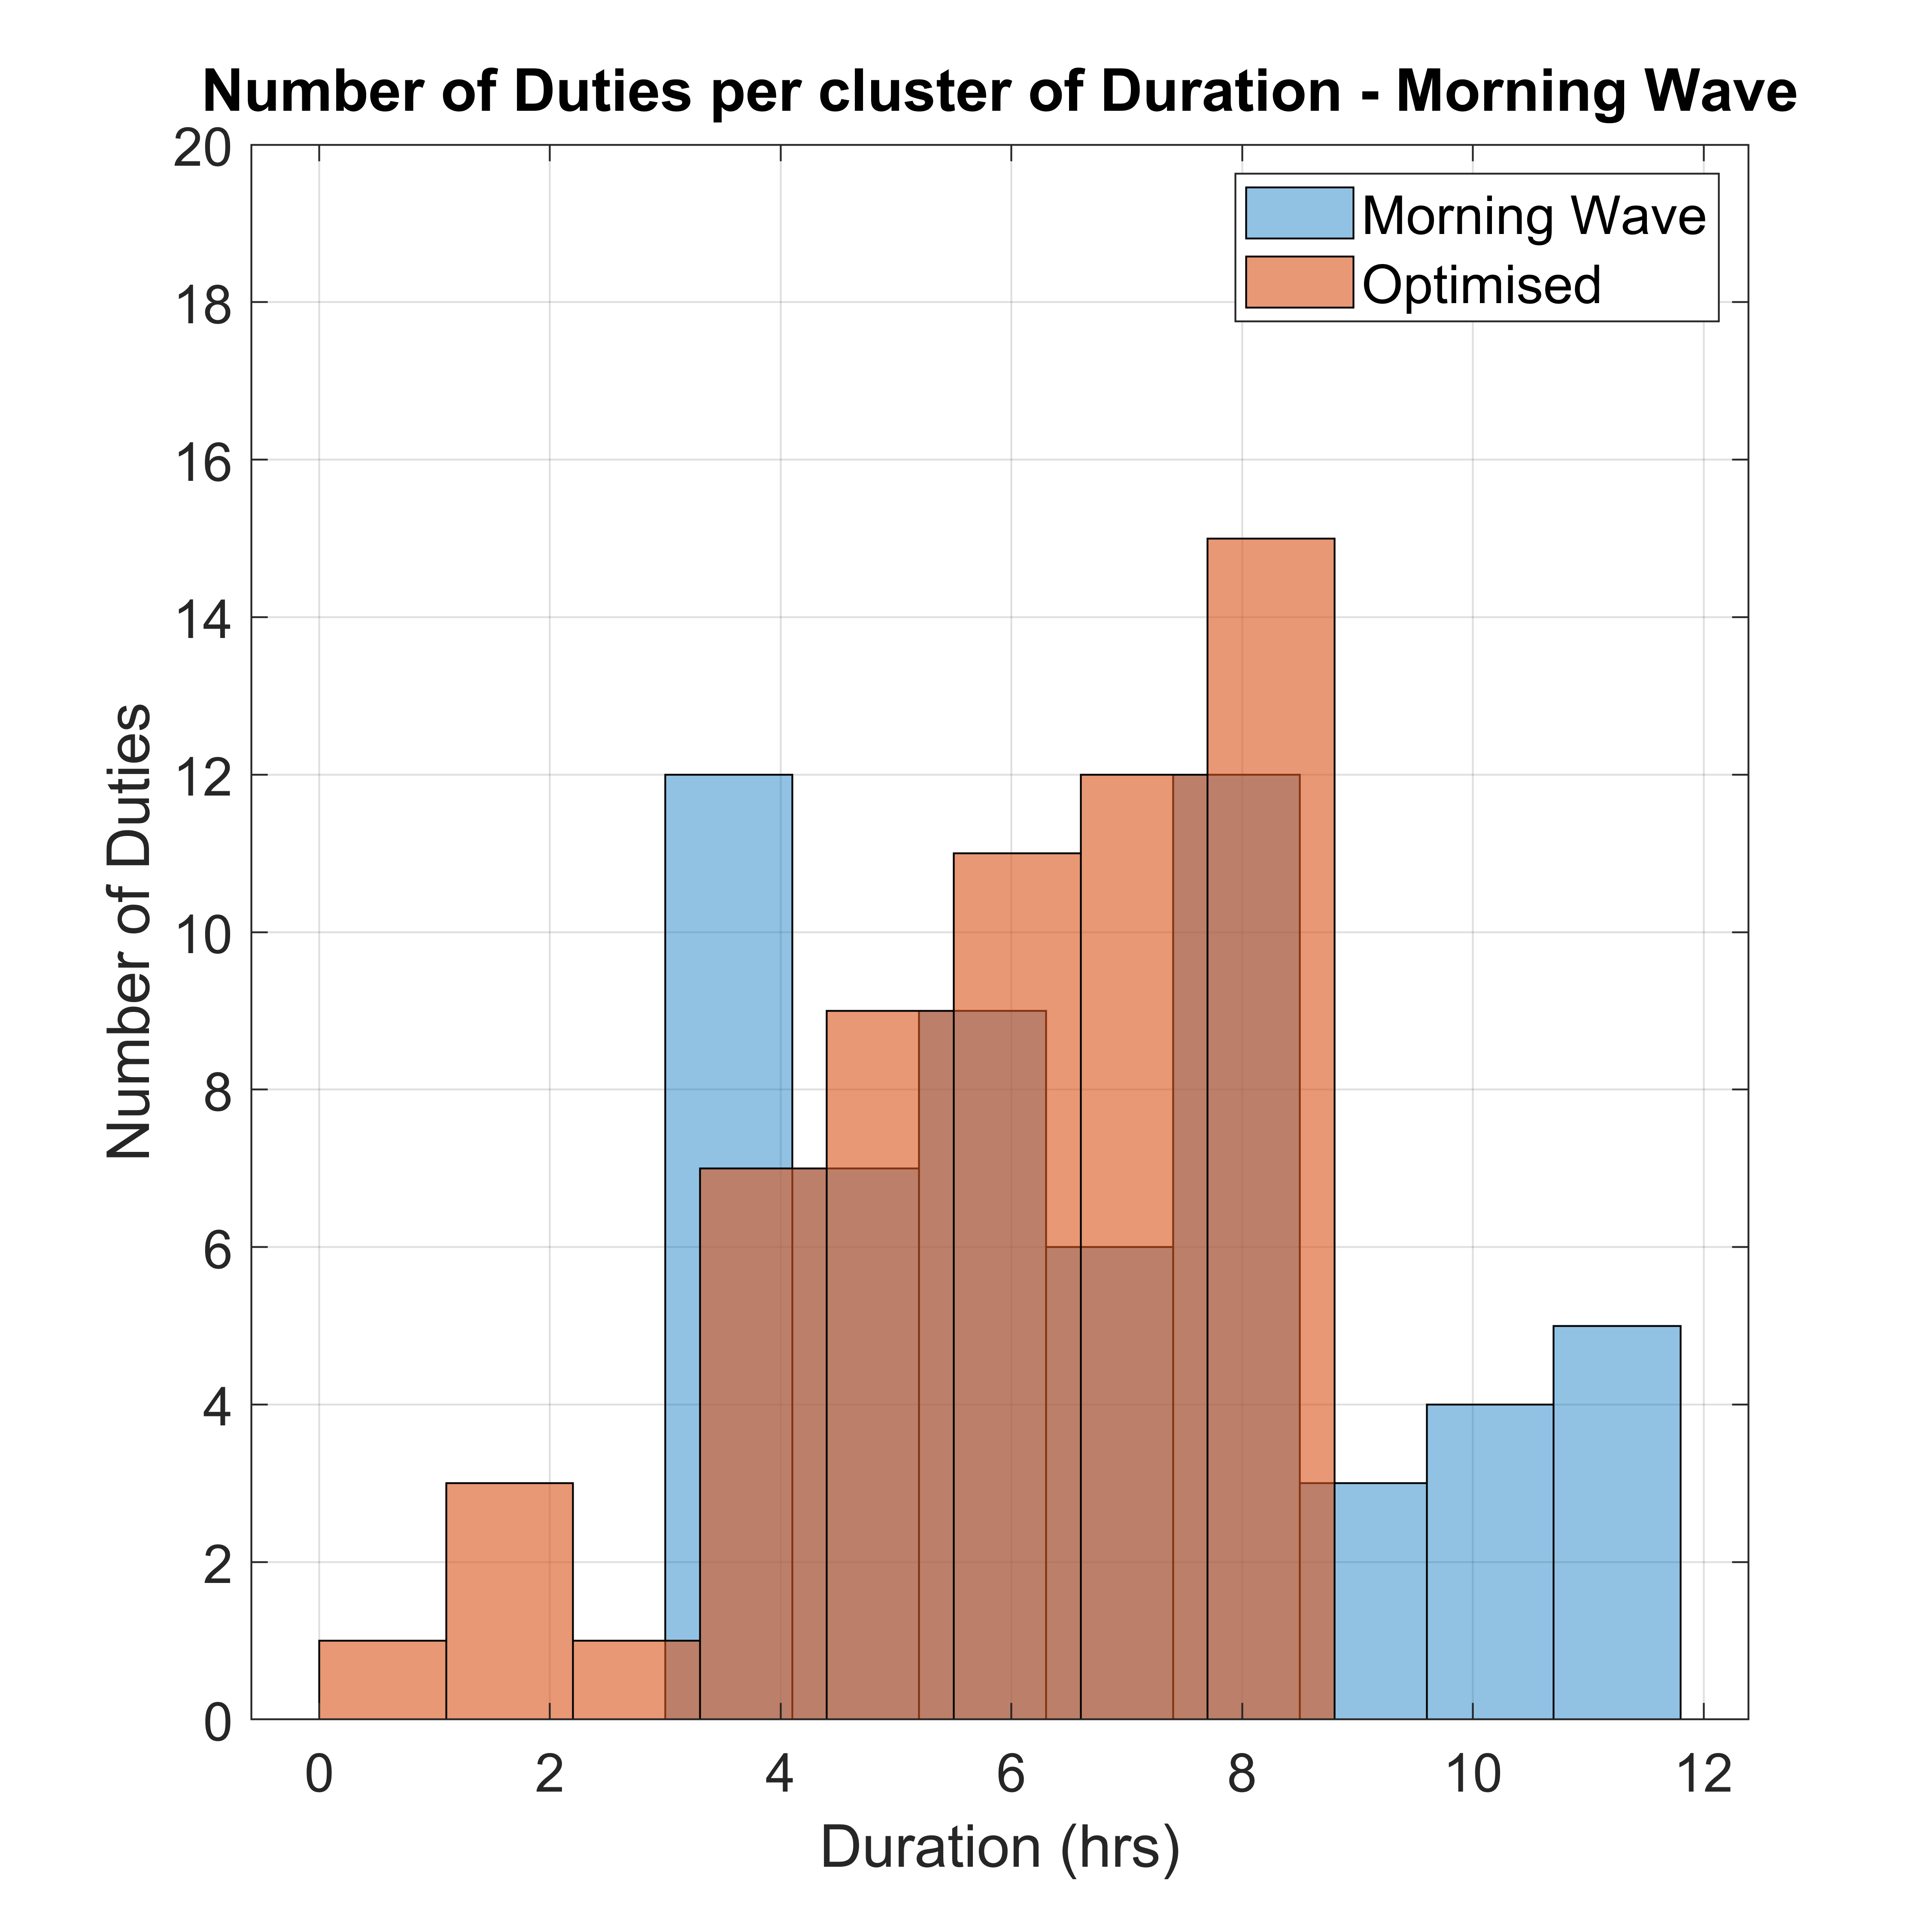
\includegraphics[width=\linewidth]{[2] - chapter/Image Files/morning.png}}
\endminipage\hfill
\minipage{0.32\textwidth}
\subfloat[Afternoon]{%\begin{center}
  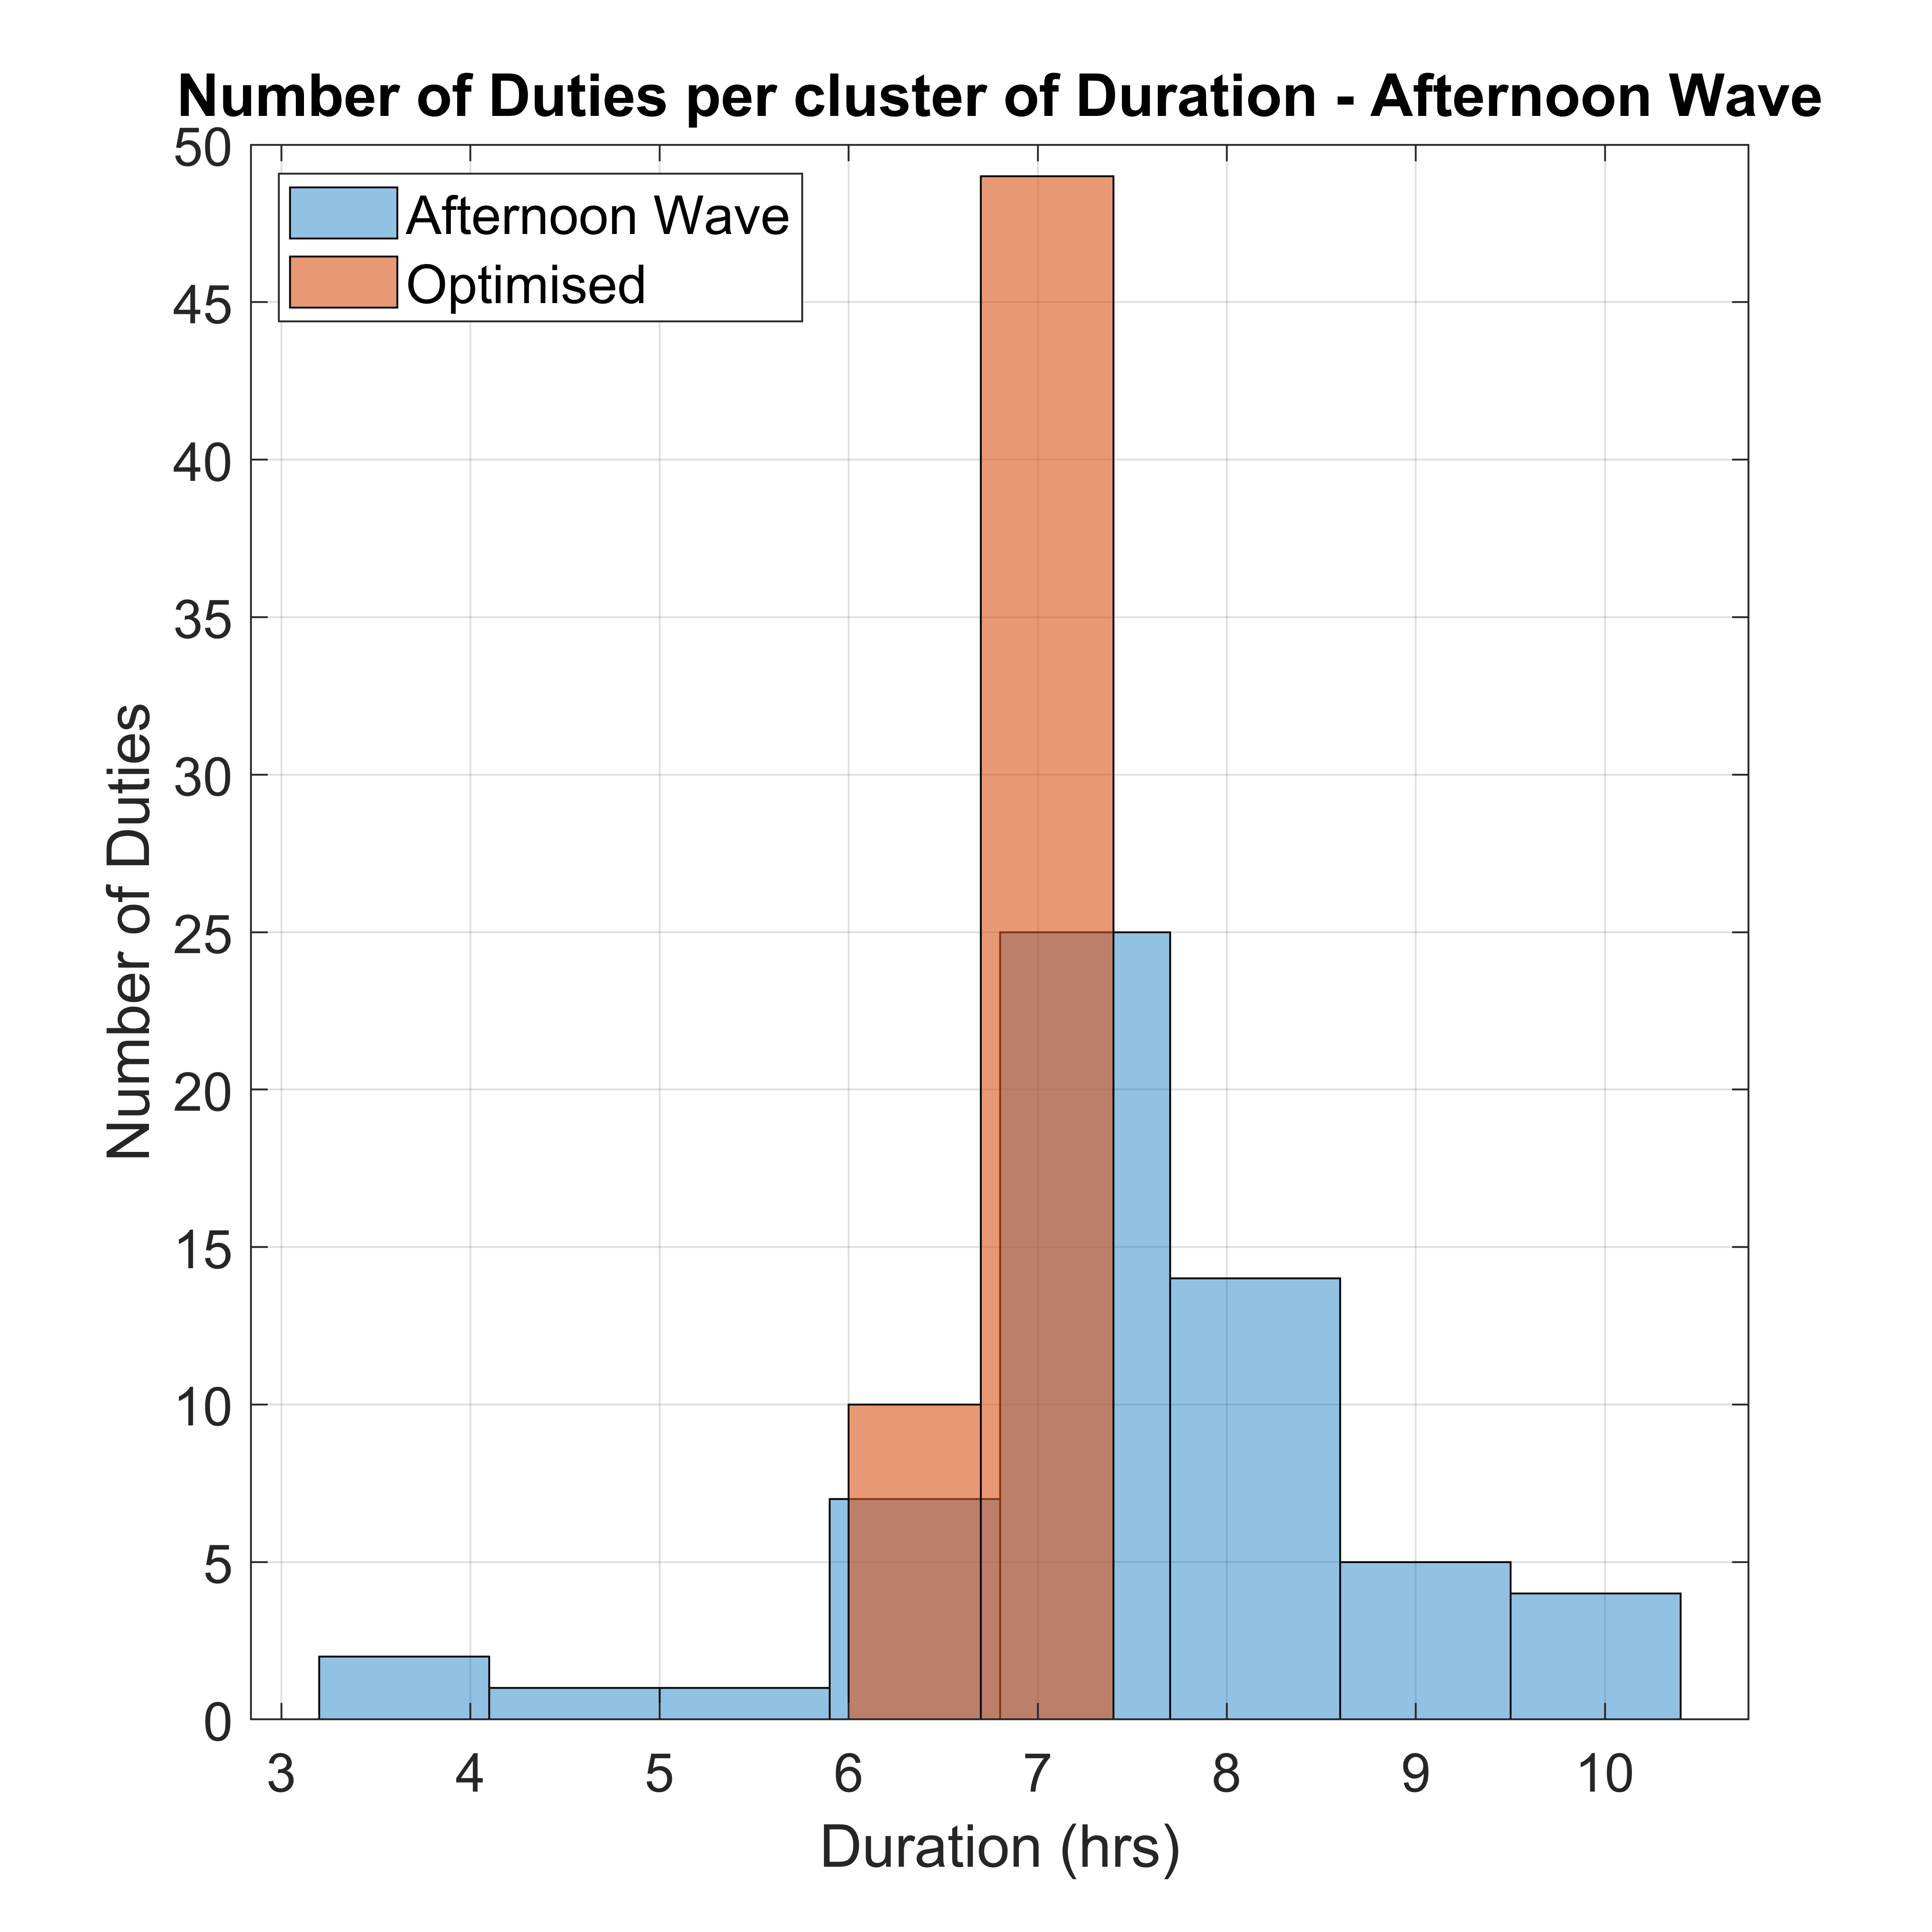
\includegraphics[width=\linewidth]{[2] - chapter/Image Files/afternoon.png}}
  
\endminipage\hfill
\minipage{0.32\textwidth}%
\subfloat[Night]{%\begin{center}
  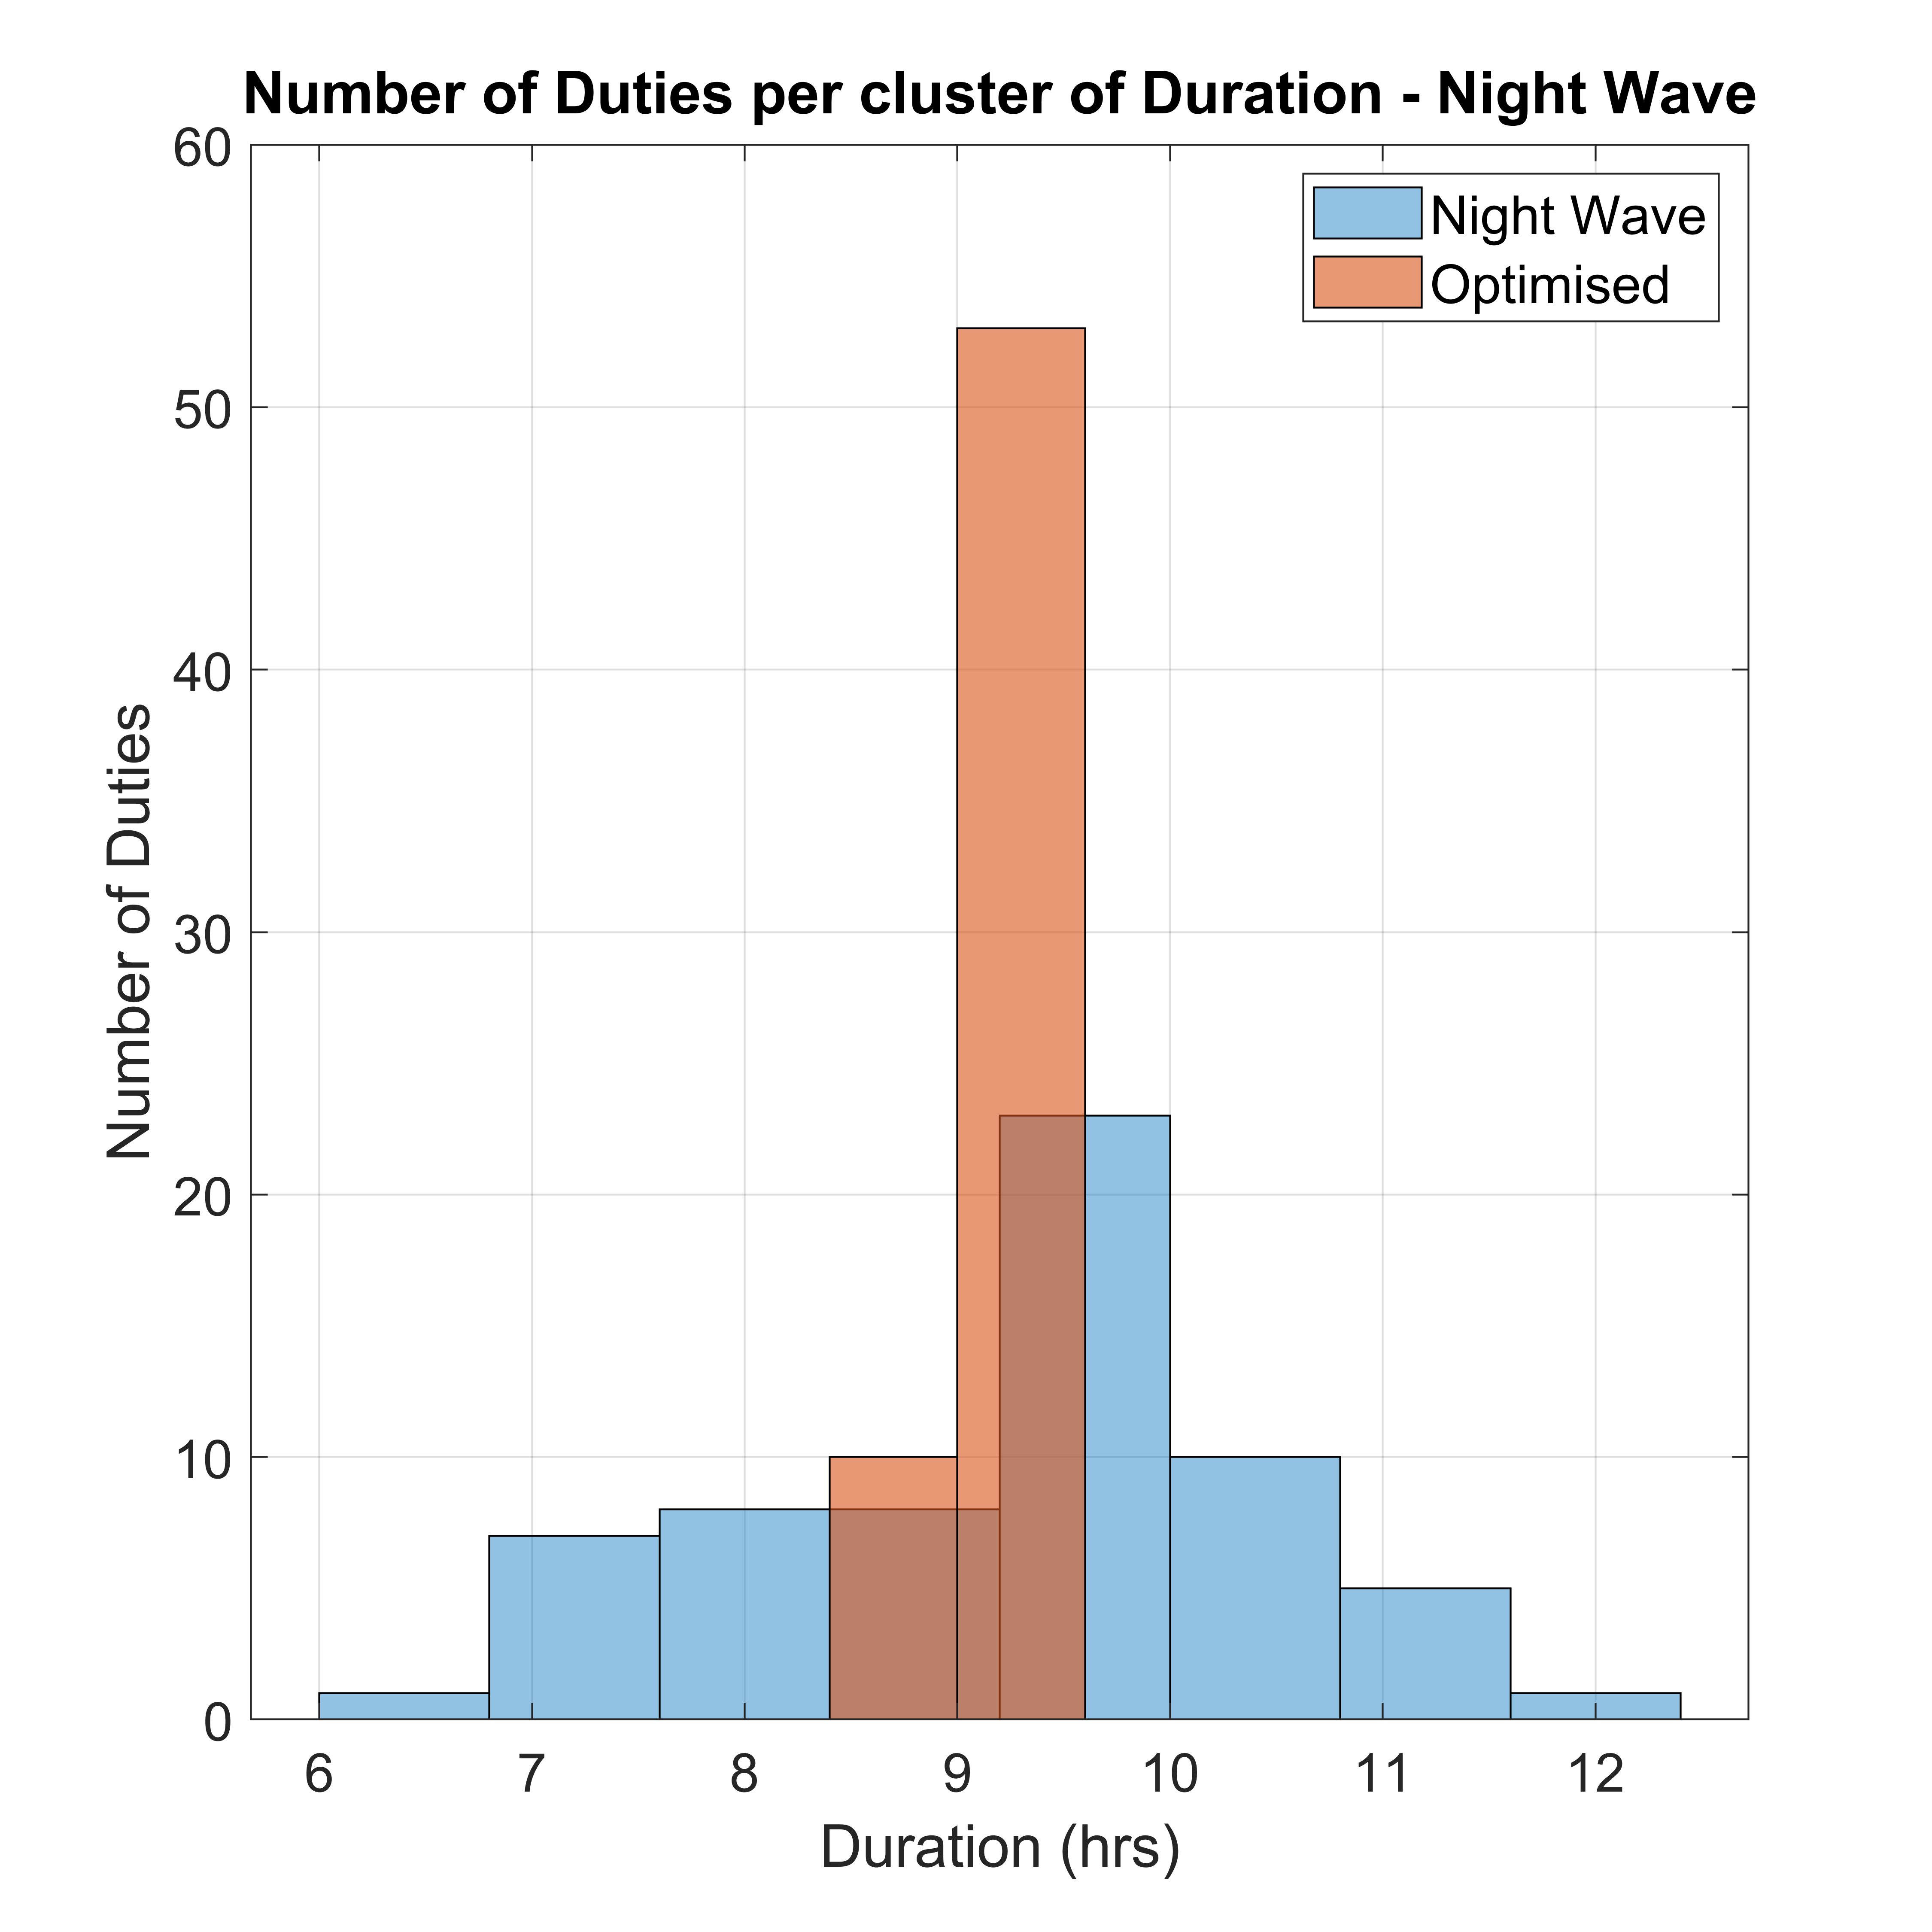
\includegraphics[width=\linewidth]{[2] - chapter/Image Files/night.png}}
 
\endminipage

\caption{The effects of Makespan Scheduling when considering our problem in Wave Instances.}
\label{fig: Wave Makespan Scheduling}
\end{figure}

\vspace{\baselineskip}
\noindent
The effects of re-organising our problem in such a fashion can be observed in Figure \ref{fig: Wave Makespan Scheduling}. Upon splitting our data into the three wave instances (\texttt{morning, afternoon, night})\footnote{The instances are listed in detail in Appendix \ref{subsection: redefine appexnix}} one can see that overall, the wave sub-instances do not consistently behave either better or worse than the schedule of the whole dataset seen previously in Figure \ref{fig:1-D1M1}(b). More specifically, in the \texttt{morning, afternoon} waves we can create schedules with a \textit{makespan} of around or below the makespan of the whole instance at the \textbf{08:25} mark, hence corroborating the fact that in an ideal schedule for the whole instance, the majority of duties should be of length below the 8 and a half hours mark obtained previously.

\vspace{\baselineskip}
\noindent
It is only in the \texttt{night} wave that we observe a sub-optimal makespan, relative to the other two. The \texttt{night} wave's makespan is beyond the 08:25 hour mark at 9 and a half hours. A sound argument behind this sub-optimal performance is to observe that the \texttt{night} wave has considerably more overall labor time to allocate than the other two instances. Moreover, it only has at most four more duties to allocate that time to, compared to the other two instances. Hence, the combination of more time to be scheduled and the limit amount of flexibility provided by the small amount of extra duties that the model has at its disposal to allocate that additional time to, lead to this sub-par performance with respect to the makespan.

\vspace{\baselineskip}
\noindent
On the other hand, the reason behind the great performance of our model in the \texttt{afternoon} instance could be zeroed down to the fact that the \texttt{afternoon} wave has the largest timespan out of the three waves (09:00-16:00), as can be seen in Table \ref{table:Starting Waves}, of Appendix \ref{subsection: Appendix Starting times}. Given, that it has a drastically bigger timespan, in fact equal to the sum of the other two instances, it might prove slightly easier to assign very late and very early starting duties since there will be more flexibility due this increased timespan.

\vspace{\baselineskip}
\noindent
Finally, we can see in Figure \ref{fig: Wave Makespan Scheduling}(a) that although the \texttt{morning} wave performs respectably with respect to its makespan, it lacks in its uniformity of the schedule compared to the other two wave instances, which enjoy a much tighter bandwidth. The non-optimised historical morning wave instance that our model receives as input could be identified as the cause for this lack of uniformity. More specifically, \ref{fig: Wave Makespan Scheduling}(a)-(c) we can see that the historical input instance for the \texttt{morning} is the least uniform out of the three. More importantly, it is \textit{right-skewed} when compared to the other two, hinting at the existence of numerous shorter-lasting shifts. As a result, our model is largely struggling to allocate the redistributed load from the longer lasting shifts to these shorter-lasting due to their small durations.  

\vspace{\baselineskip}
\noindent
These individual findings for each wave sub-instance justify the fact that the most frequently occurring duties in the whole dataset tend to have a duration between 6-8 hours. In addition, it is the shifts of the \texttt{night} wave, which contain the biggest portion of schedulable time, that end up contributing to pushing the makespan beyond 6 hours up to the 08:25 mark. 

\vspace{\baselineskip}
\noindent
All in all, by approximating the real-world through adding such constraints to our problem that make it more realistic in terms of its ease of implementation, for our Industrial Liaison, we have determined that the efficiency of our schedules is \textbf{not} significantly \textbf{compromised}. The \textit{makespan}, of the optimal schedule compared to that of the historical one is \textbf{equal or smaller} for two of the three waves. In addition, the optimised schedules are much more \textbf{uniform} than their historical equivalent, as seen in the table below\footnote{Each wave-optimised schedule is compared with its wave sub-instance for the table's evaluation criteria. Effectively, for each chart of Figure \ref{fig: Wave Makespan Scheduling} we compare the optimised schedule with the input wave instance.}:

%%%%%%%%%%%%%%%%%%%%%%%%%%%%%%%%%%%%%%%%%%%%%%%%%%%%%%%%%%%%%%%%%%%%%% Table %%%%%%%%%%%%%%%%%%%%%%%%%%%%%%%%%%%%%%%%%%%%%%%

\begin{table}[h]
\small
    \centering 
\begin{tabular}{l|c|c}
        \textbf{Schedule} & \textbf{Makespan Reduction (\%)} & \textbf{Maximum Difference-Reduction (\%)} \\
        \hline
         Historical\_Optimised & 28\% & 72\% \\
        \hline
         Morning\_Optimised  & 28\% & 14\% \\ 
         \hline
         Afternoon\_Optimised  & 29\% & 76\% \\ 
         \hline
         Night\_Optimised  & 19\% & 80\% \\ 
\end{tabular}
\end{table}

%%%%%%%%%%%%%%%%%%%%%%%%%%%%%%%%%%%%%%%%%%%%%%%%%%%%%%%%%%%%%%%%%%%%%%%%%%%%%%%SECTION%%%%%%%%%%%%%%%%%%%%%%%%%%%%%%%%%%%%%%%%%%%%%%%%%%%%%%%%%%%%%%%%%%%%%%%%%%%%%%
\section{Trade-off between Number of Completed Duties and Maximum Duty Length}
\label{section:minimise duties}
Upon proving that there exists significant room for improvement with respect to the historical schedule's makespan we re-examined the historical schedule to see if there are other aspects of it that could be improved. After a careful observation of the dataset we noticed that there are potentially too many duties in the historical schedule. Consequently, people have to work a lot to carry out all those duties. To remedy this, we attempt to minimise the number of duties that are required to complete the same amount of workload (i.e. same amount of blocks). 

\vspace{\baselineskip}
\noindent
Provided we are able to decrease the number of duties for the same amount of blocks, this would translate to people working less, since there would be less duties requiring completion. In practical terms this amounts to a transformation of our problem to a Bi-Objective Generalised Assignment Problem \cite{PRAKASH2010} since it aims to \textbf{minimise} the \textbf{maximum duty length}, while also \textbf{minimising} the \textbf{number of duties}. 

\vspace{\baselineskip}
\noindent
To solve this problem we need to develop an algorithm that will provide us with the Pareto Optimal points of the problem. Those points will represent Pareto Optimal schedules, and our Industrial Partners can evaluate each of those schedules to select the one that best fits their company policy requirements. We rely upon the formulation of the previous section but shift the focus of the minimisation problem onto minimising the number of duties that need to be operational to carry out the required tasks. We hypothesise that we can fix an upper threshold for the duty length ($L$). We hence assume that people have to work $L$ hours, and not any more than that. 

\vspace{\baselineskip}
\noindent
For the purposes of our solver that means that it can schedule duties that are only as long as that threshold. The solver hence, has at its disposal duties that are subject to this upper bound to and has to attempt to fit all the blocks inside of them. In practice this is enforced by creating a constraint that applies this upper bound restriction to the duties' lengths. We hence, take the minimisation of the duration out of the objective function of this problem but it remains in spirit as the secondary objective that we will attempt to minimise through our sensitivity analysis.

\vspace{\baselineskip}
\noindent
The variable $y_{i}$ contains a value that specifies the number of duties $i$ that are \textbf{required}. Similarly to the previous formulation binary variable $x_{i,j}$ dictates the assignment of a block $j$ to a duty $i$ and is equal to 1 if the atomic block $j \in B$ is assigned to duty $i \in D$, and 0 otherwise.

%%%%%%%%%%%%%%%%%%%%%%%%%%%%%%%%%%%%%%%%%%%%%%%%%%%%%%%%%%%%%%%%%%%%%%%%%%%%%%% Maths %%%%%%%%%%%%%%%%%%%%%%%%%%%%%%%%%%%%%%%%%%%%%%%%%%%%%%%%%%%%%%%%%%%%%%%%%%%%%%

\vspace{\baselineskip}
\begin{equation}
\label{equation: Minimise Duties}
\begin{aligned}
&\text{minimise}
& & \sum _{i=1}^m y_{i}  \\
& \text{subject to}
& & y_{i} \geq x_{i,j}  \;\;\; &\forall \; i \in D,\; j \in B\\   
& & &\sum _{i=1}^m x_{i,j} = 1 \;\;\; &\forall \; j \in B\\
%& & &\sum _{j=1}^n x_{i,j}p_{j} \leq f_{i}-s_{i} \;\;\; &\forall \; i \in D\\
& & &\sum _{j=1}^n x_{i,j}p_{j} \leq L \;\;\; &\forall \; i \in D\\
& & & y\geq 0  \\
& & & x_{i,j} \in  \{ 0,1 \} \;\;\; &\forall \; j \in B, \; i \in D\\
\end{aligned}
\end{equation}

\vspace{\baselineskip}
\noindent
The model minimises the number of active duties. The first constraint makes sure that a duty $i$ is counted as active if at least one of the $x_{i,j}$ is equal to 1. The second constraint makes sure that each atomic block is executed by one and only one duty. Finally, the third constraint makes sure that the contents of a duty do not exceed the maximum duty length threshold $L$. This maximum duty length is determined by the hyper-parameter $L$ that we supply as input to the model 36 times to complete the sensitivity analysis. 

%%%%%%%%%%%%%%%%%%%%%%%%%%%%%%%%%%%%%%%%%%%%%%%%%%%%%%%%%%%%%%%%%%%%%%%%%%%%%%% sub-SECTION %%%%%%%%%%%%%%%%%%%%%%%%%%%%%%%%%%%%%%%%%%%%%%%%%%%%%%%%%%%%%%%%%%%%%%%%%%%%%%

\subsection*{Evaluation}
\vspace{\baselineskip}
\noindent
Using this formulation we investigate the number of active duties that can be reduced for various levels of the maximum duty length. This investigation is carried out by conducting a sensitivity analysis, where we vary the hyper-parameter $L$ and measure the number of duties required. A particularly important threshold that we choose to focus on is that of setting \textit{L} equal to the maximum duty length observed in the historical schedule. This will allow us to determine the optimal number of duties that could have been used instead of the historically used 183 duties utilised by Royal Mail. 

%%%%%%%%%%%%%%%%%%%%%%%%%%%%%%%%%%%%%%%%%%%%%%%%%%%%%%%%%%%%%%%%%%%%%%%%%%%%%%% Figure %%%%%%%%%%%%%%%%%%%%%%%%%%%%%%%%%%%%%%%%%%%%%%%%%%%%%%%%%%%%%%%%%%%%%%%%%%%%%%

\begin{figure}%
    \centering
    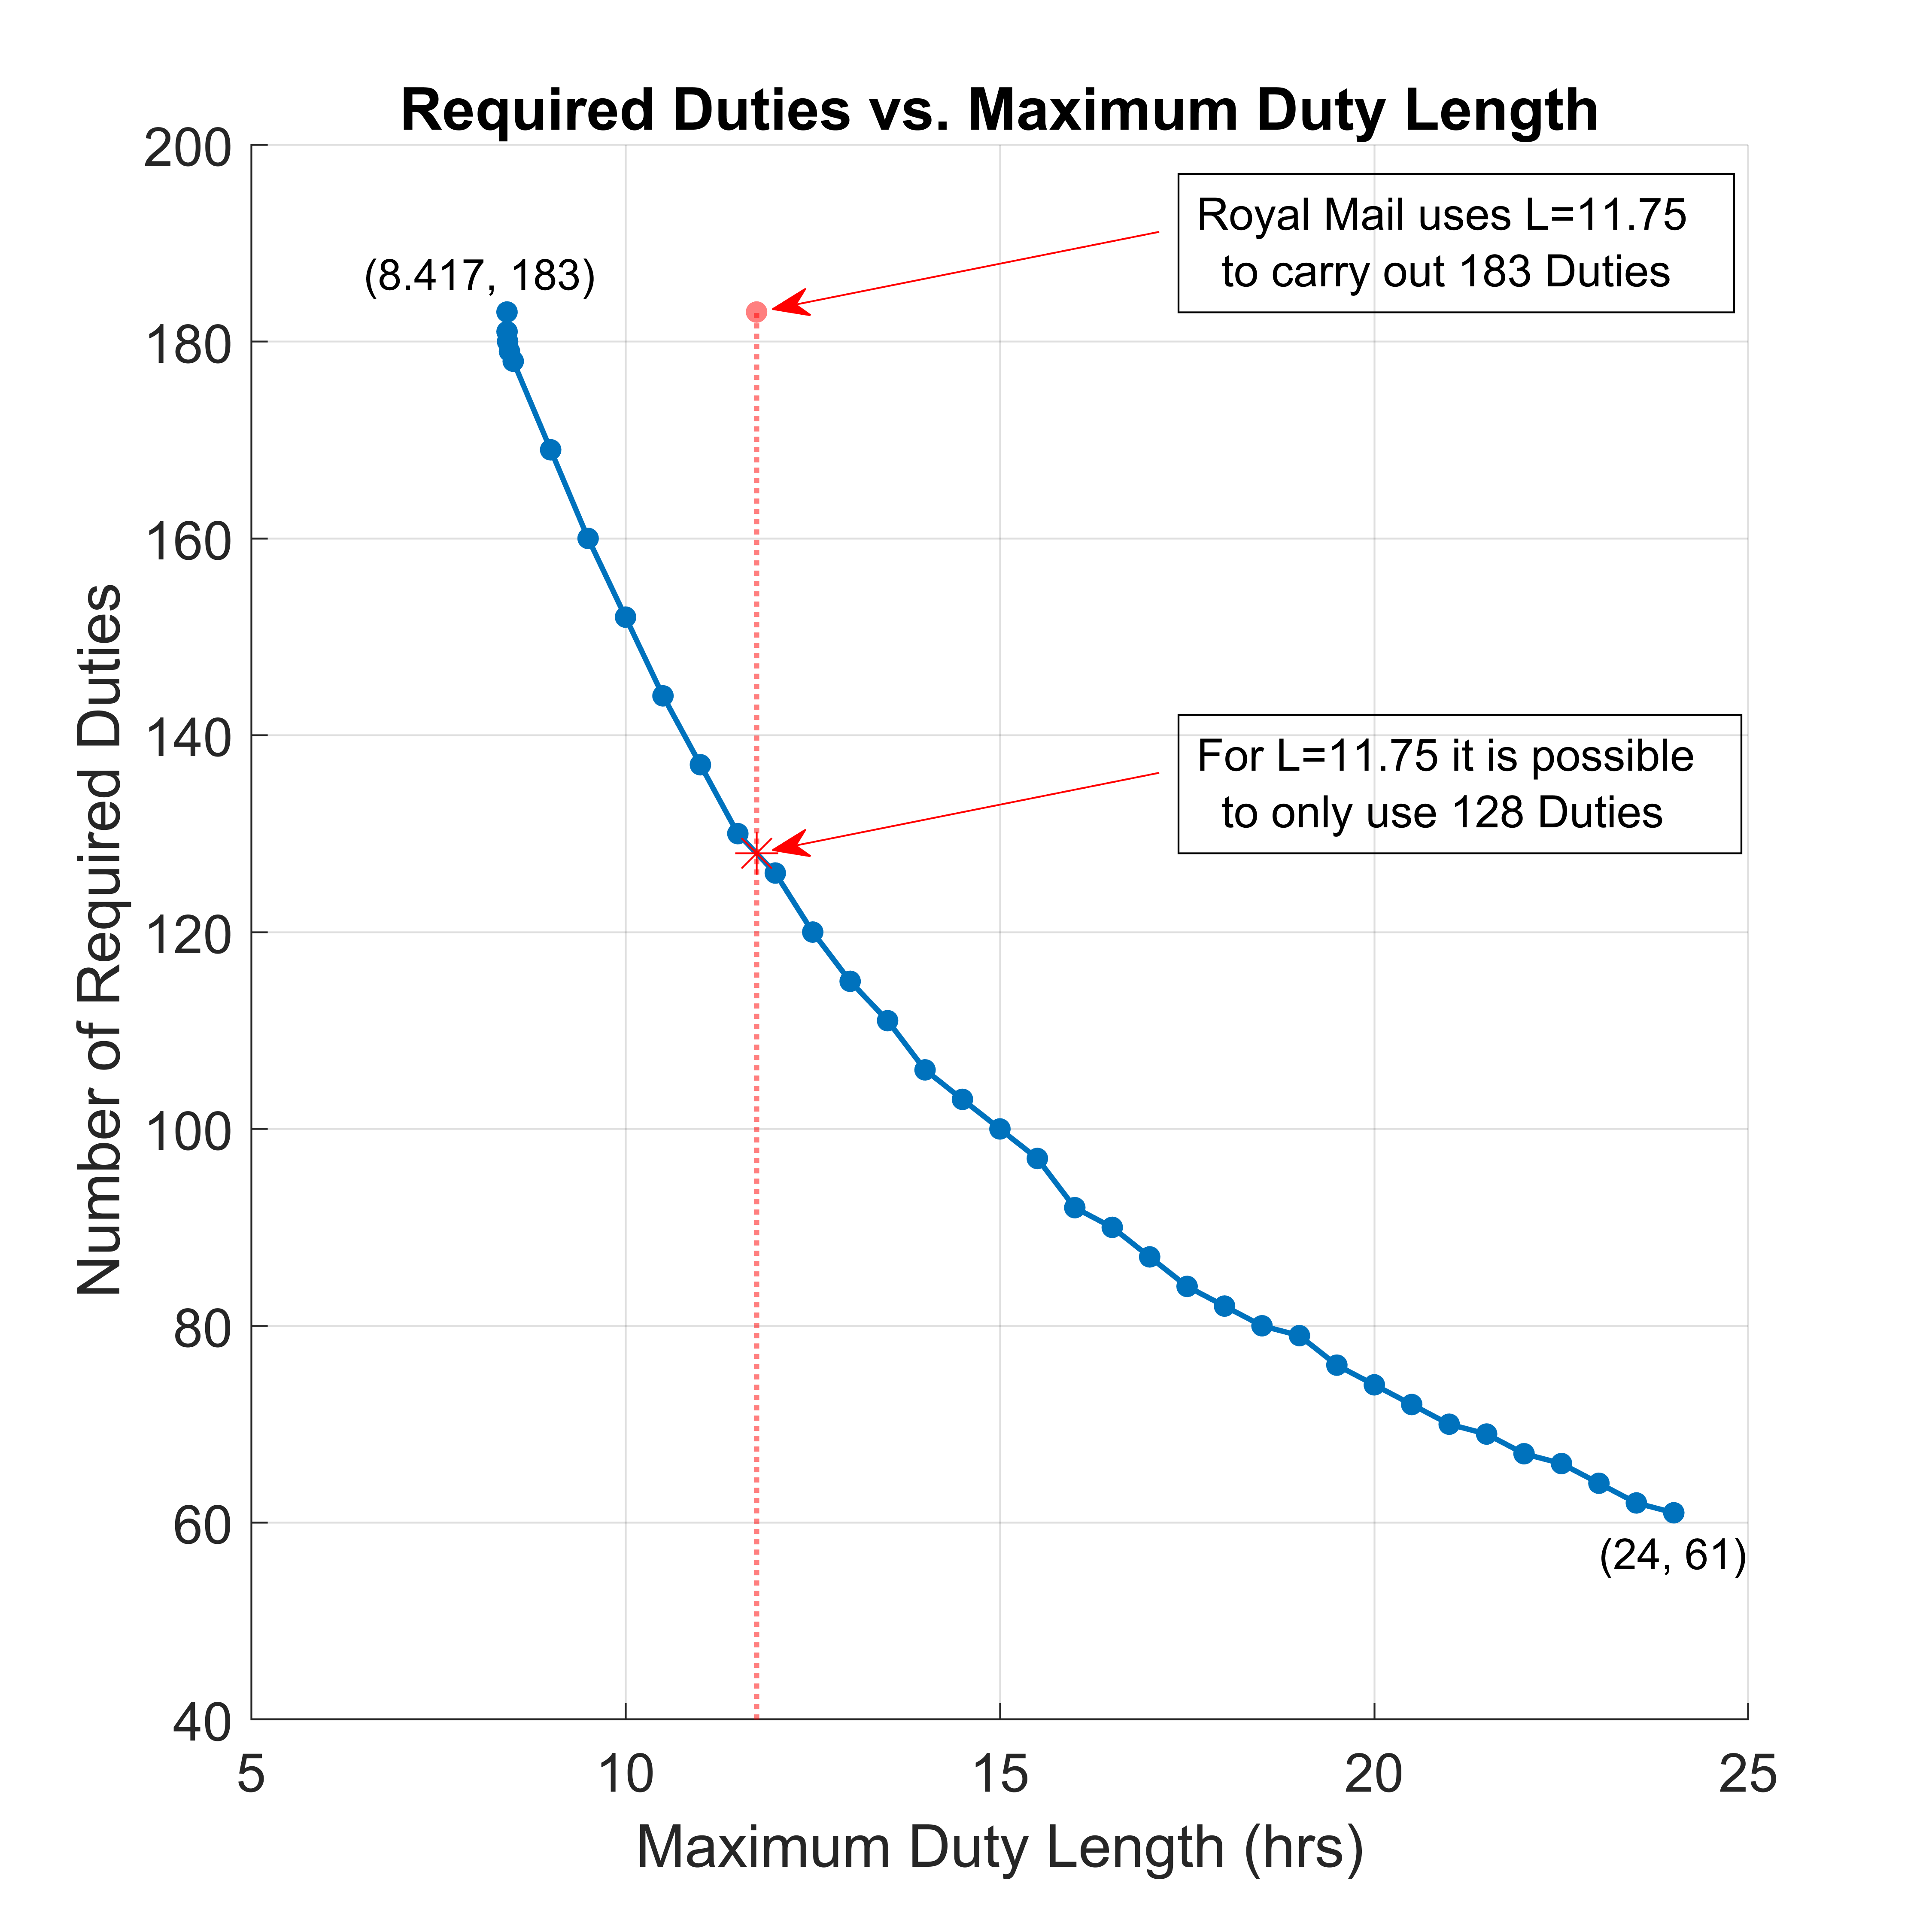
\includegraphics[width=0.46\linewidth]{[1] - chapter/Image Files/1-D1M2.png}
    \caption{Depicts the number of duties required as a function of the Maximum Duty Length varied in 30 minute intervals, up to an \textit{upper threshold} of \textbf{24 hours} per duty.}
    \label{fig:1-D1M2}
\end{figure}

%%%%%%%%%%%%%%%%%%%%%%%%%%%%%%%%%%%%%%%%%%%%%%%%%%%%%%%%%%%%%%%%%%%%%%%%%%%%%%% sub-SECTION %%%%%%%%%%%%%%%%%%%%%%%%%%%%%%%%%%%%%%%%%%%%%%%%%%%%%%%%%%%%%%%%%%%%%%%%%%%%%%

\subsubsection*{Qualitative Results}
In Figure \ref{fig:1-D1M2} we plot the result of the sensitivity analysis. In more detail, through utilising the principle of the Pareto front we computed the efficient frontier seen in Figure \ref{fig:1-D1M2} by applying algorithm (\ref{alg: Pareto}) 36 times\footnote{\label{Pareto}Seen in Section \ref{section: Pareto} of Chapter \ref{chapter: Background}} between a minimum and maximum \textit{L}. Hence, the trade-off curve shows the sensitivity analysis in its entirety applying the Pareto algorithm from a maximum \textit{L} of 24 hours down to a minimum \textit{L} of around 8 and half hours, that still provides a feasible schedule. Obviously, we cannot expect an individual to complete duty lasting 24 hours, however, we present the Pareto front to allow the flexibility for our industrial partner. Figure \ref{fig:1-D1M2} shows that if the maximum duty length increases the number of duties required decreases significantly. 



%%%%%%%%%%%%%%%%%%%%%%%%%%%%%%%%%%%%%%%%%%%%%%%%%%%%%%%%%%%%%%%%%%%%%%%%%%%%%%% sub-SECTION %%%%%%%%%%%%%%%%%%%%%%%%%%%%%%%%%%%%%%%%%%%%%%%%%%%%%%%%%%%%%%%%%%%%%%%%%%%%%%

\subsubsection*{Quantitative Results}
As mentioned before although it might not be directly reflected in equation (\ref{equation: Minimise Duties}) this is principally a Bi-Objective problem where the two objectives minimised are the maximum duty length (\textit{L}) and the number of duties. As result, on the left end of the curve one can see the value of \textit{L} for which the objective regarding the minimisation of \textit{L} is best satisfied. As observed in Figure \ref{fig:1-D1M2} that minimal value of \textit{L} is equal to 8.417 hours\footnote{Which amounts to 8 hours and 25 minutes.} and this allows us to complete all blocks in the original 183 duties. Hence, we have identified an optimisation opportunity since it is possible to allocate the same workload into a schedule with \textbf{shorter maximum lasting duty} compared to the historical practices. A careful observer will recognise that this exact finding was been seen in an earlier stage of this report. Namely, this value for the maximum duty length, coincides exactly with the value found for the Makespan of the optimal schedule in Section \ref{section:Makespan Scheduling-content}. Consequently, we can be sure that the schedule with $L=8.417 \text{ hours}$ is a Pareto optimal schedule that satisfies the minimisation of the maximum duty length objective of this problem.

\vspace{\baselineskip}
\noindent
Moreover, looking at the rest of the curve we can see that we have determined that we are able to reduce the amount of duties required significantly, as we increase hyper-parameter $L$. Using the \textit{L}-\textbf{threshold} of around 12 hours currently utilised by Royal Mail allows us to use a mere 128 duties compared to the 183 required by Royal Mail. This translates to a \textbf{30\%} reduction in the duties that need to be fulfilled for the same maximum duty length (\textit{L)}. Practically this means that if a small portion of the drivers is able to complete overtime duties (up to that 12 hours threshold) the remaining cohort of drivers would be able to work less since there would be less duties to be completed. 


\vspace{\baselineskip}
\noindent
The realisation that Royal Mail's current operating scenario is not on the Pareto frontier, is another indication that there is a substantial need for optimisation that will most likely lead to opportunities for cost cuts once Royal Mail places itself on the frontier. Taking into account the reality-based constraints that would constrict the provision of more efficient scheduling, we proceed to propose the most optimal but realistic schedule that Royal Mail can aim towards. That practical limit is founded in the fact that the maximum number of labor hours per day for an individual is a total of 13 hours as determined by EU rules\footnote{Seen in Appendix \ref{section: EU rules}}. If we proceed to utilise a maximum duty length $(L)$ of 13 hours the Pareto optimal schedule that we can achieve requires merely 115 duties to be completed. This would be a significant decrease over the 183 duties of the historical solution.

\vspace{\baselineskip}
\noindent
Finally, looking at the \textbf{theoretical optimal schedule} with respect to the other objective of this problem (i.e. minimal \textit{L}) we claim in theory we can do even better than a schedule with $L=8.417 \text{ hours}$. The most optimal schedule that we can hope to achieve is a schedule with a maximum duty length equal to that of the average duty duration of the input instance. That is because such a schedule would be equivalent to spreading the total schedulable hours equally to all 183 available duties. The historical schedules contained 183 duties with an average duty length 7 hours and 50 minutes, equivalent to 1435 hours and 22 minutes of total workload. We can see that the lowest feasible threshold for our maximum duty length in Figure \ref{fig:1-D1M2} is that of 8 hours and 25 minutes. This indicates that there an optimality gap between the ideal maximum duty length and the practical one. This is to be expected, due to the fact that the theoretical optimum could only be achieved if we neglect assumption (1) from Section \ref{section: 4.1}. In reality the atomic blocks in the input instance have an arbitrary size and hence we cannot obtain an exact fit of the blocks to all duties that sums to 7 hours and 50 minutes.

%%%%%%%%%%%%%%%%%%%%%%%%%%%%%%%%%%%%%%%%%%%%%%%%%%%%%%%%%%%%%%%%%%%%%%%%%%%%%%% Figure %%%%%%%%%%%%%%%%%%%%%%%%%%%%%%%%%%%%%%%%%%%%%%%%%%%%%%%%%%%%%%%%%%%%%%%%%%%%%%

\begin{figure}%
    \centering
    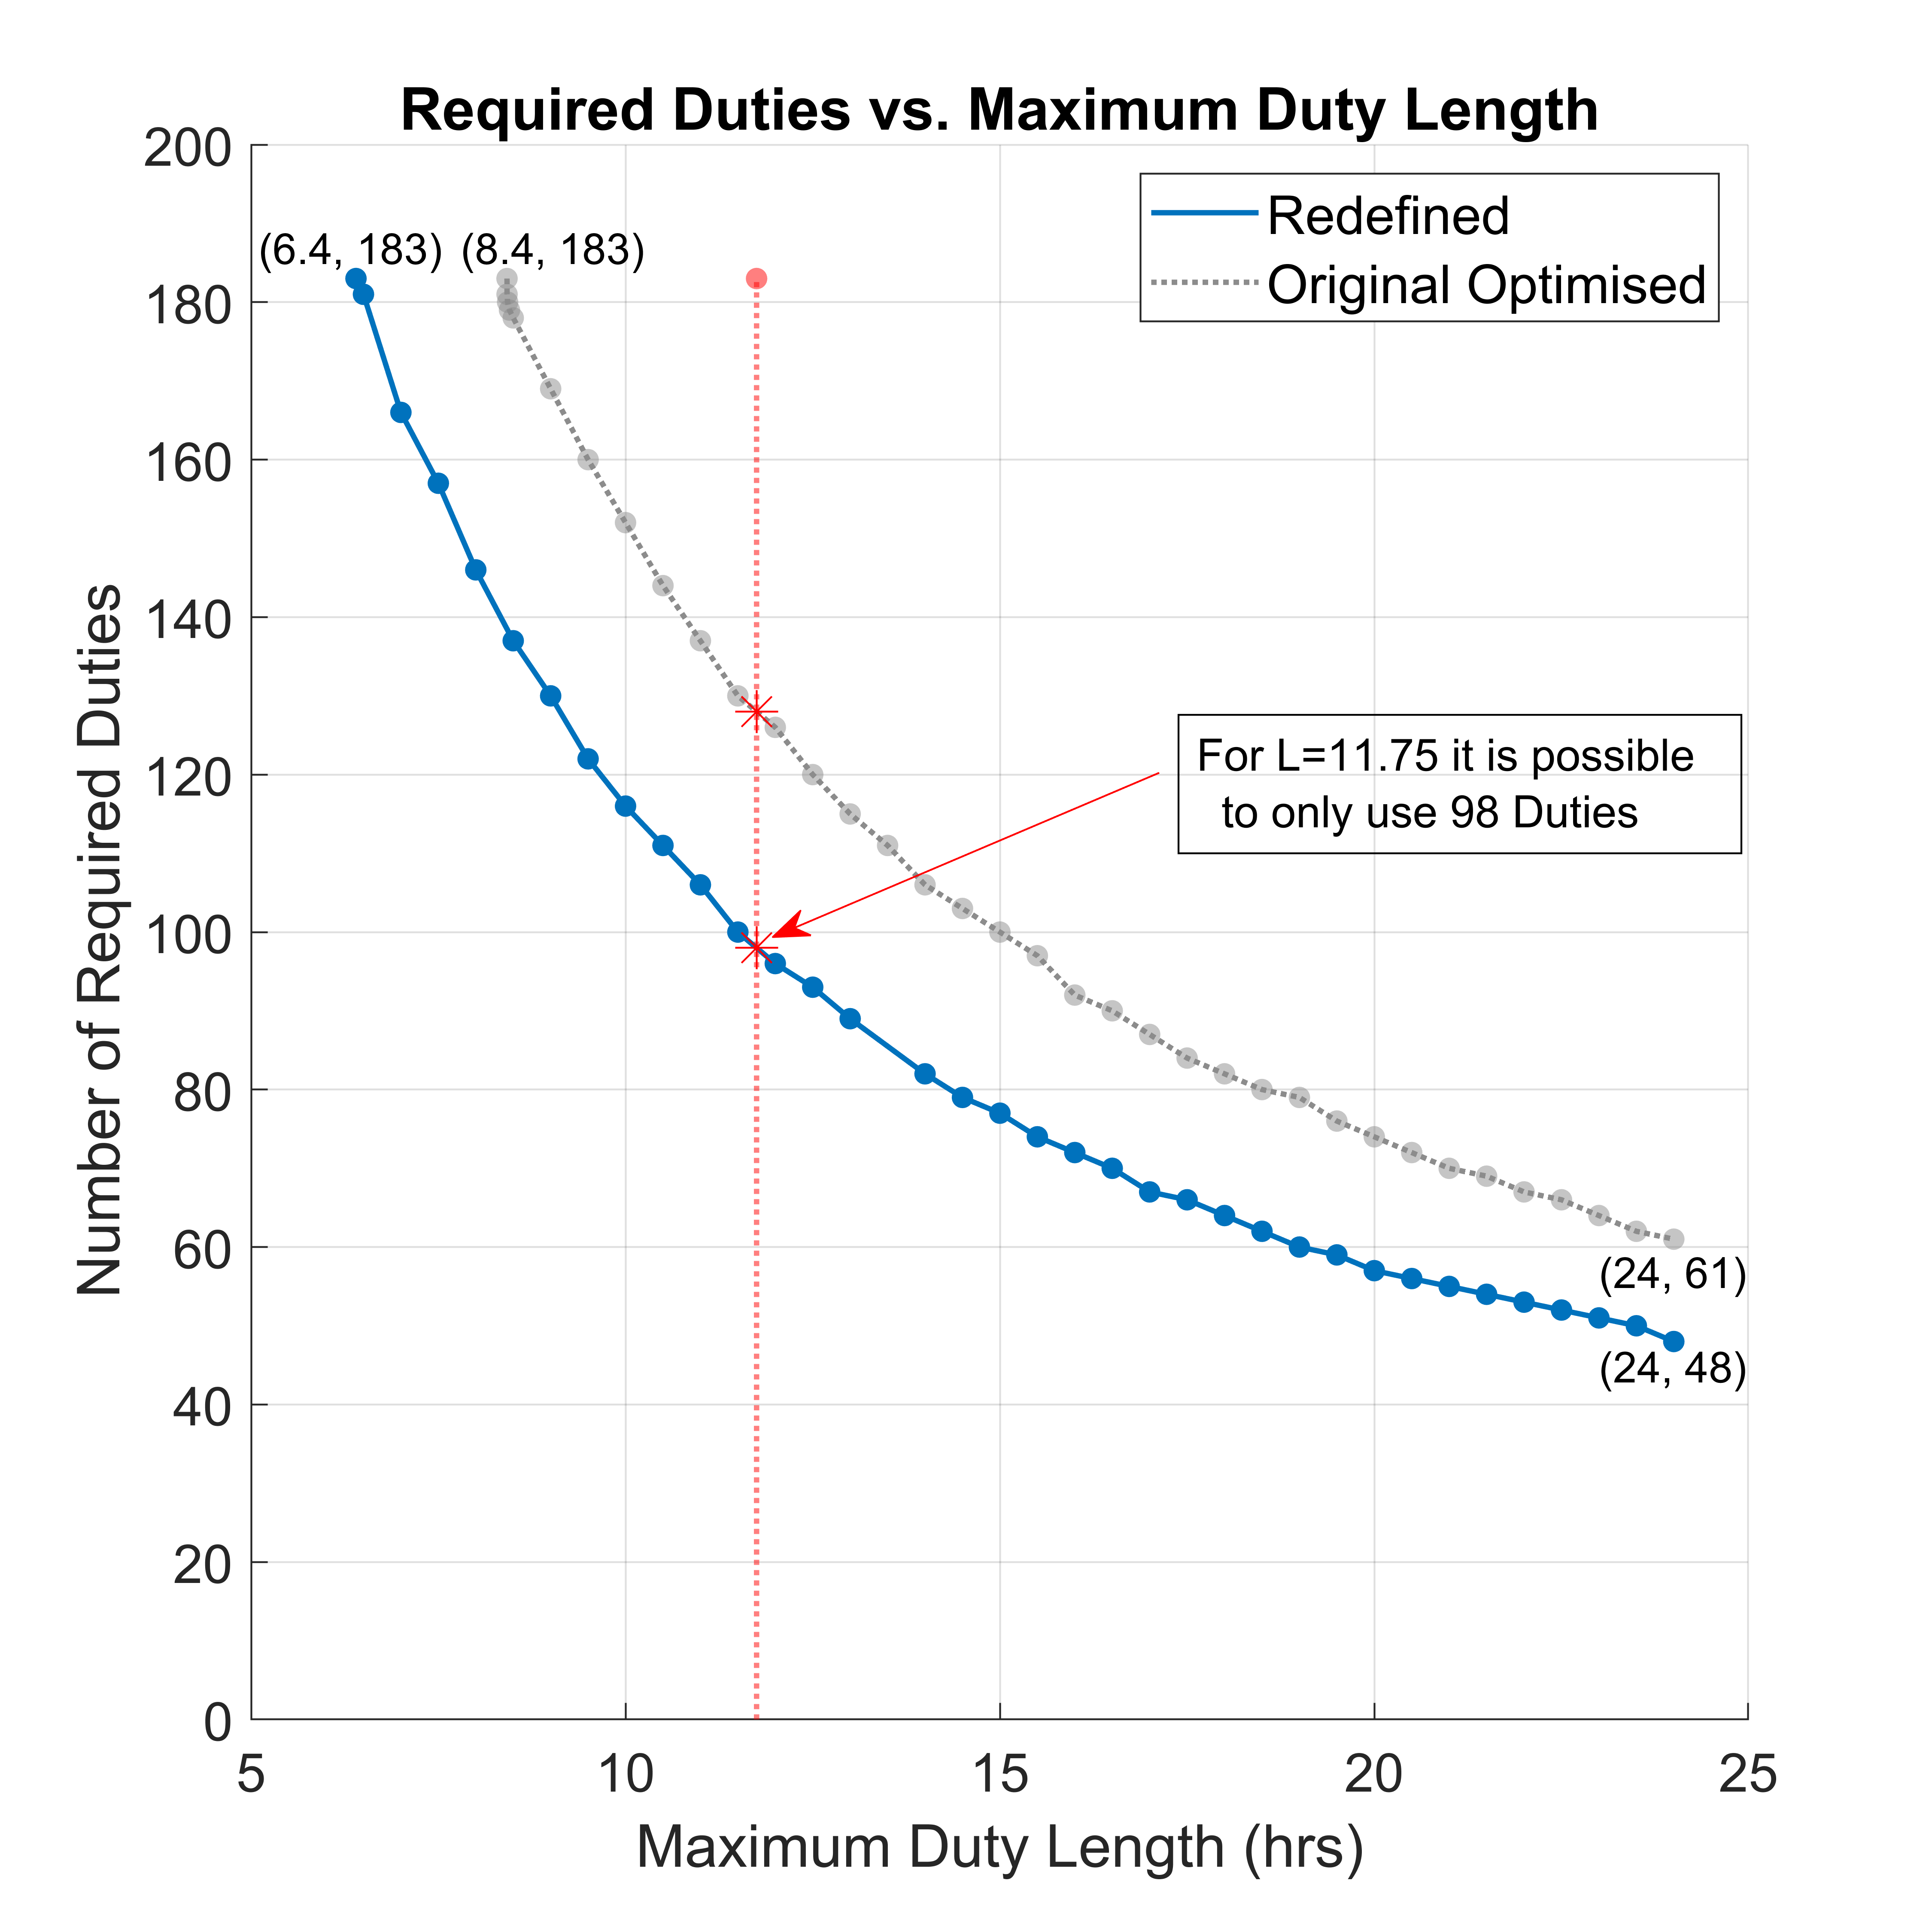
\includegraphics[width=0.46\linewidth]{[1] - chapter/Image Files/1-D2M2.png}
    \caption{Compares the number of duties required as a function of the Maximum Duty Length for the Redefined and Historical instances.}
    \label{fig:1-D2M2}
\end{figure}


%%%%%%%%%%%%%%%%%%%%%%%%%%%%%%%%%%%%%%%%%%%%%%%%%%%%%%%%%%%%%%%%%%%%%%%%%%%%%%% sub-SECTION %%%%%%%%%%%%%%%%%%%%%%%%%%%%%%%%%%%%%%%%%%%%%%%%%%%%%%%%%%%%%%%%%%%%%%%%%%%%%%


\subsection*{Evaluation - Optimising Redefined Instance}
We proceed to apply the Redefined instance, to model (\ref{equation: Minimise Duties}) in order to determine whether applying this more realistic instance will further improve the two objectives of our problem. For the historical instance, our optimisation was able to minimise the number of duties by around 30\% for an \textit{L} equal to Royal Mail's historical threshold. When applying the Redefined instance we expect an additional decrease in the number of required duties for the same \textit{L}. The expectation is founded in the fact that, in this new instance there is less overall schedulable time. Hence, that means that for the same maximum duty length, we can fit more blocks per duty which will directly result in less duties being used overall. 

\vspace{\baselineskip}
\noindent
Indeed, were able to carry out the same amount of block with \textbf{47\%} less duties, namely merely 96 duties as seen in Figure \ref{fig:1-D2M2}. This result justifies our quest for optimisation, since it identifies that Royal Mail's current practices are once again outside the \textit{efficient frontier} line. 

\vspace{\baselineskip}
\noindent
Observing the Figure \ref{fig:1-D2M2}, we can see that this additional reduction in required duties, is mostly due to the step change in \textit{idle time} that we are able to achieve from deleting the \textit{non-useful} activities within the blocks. However, as is shown in Section \ref{section: Redefined Dataset} the idle time that we gain is on average 1 hour and 44 minutes per duty. Moreover, we saw in Section \ref{section:Makespan Scheduling-content} that the average size of a block is on average 2 hours and 25 minutes for the Redefined instance. As a result of those two facts we can determine why the application of the model on the Redefined yields only an additional small improvement of 17\% in the number of duties deleted compared to the 30\% improvement obtained in the Historical instance. The explanation is found in the fact despite the increase in idle time there is still not enough space to re-allocate the deleted duties' blocks to other duties, since the average idle time gain (of 01:44) per duty, is significantly smaller than the average size of the block (02:25), hence there are generally not too many blocks that can be relocated to other duties so that we can delete their original duty.


\vspace{\baselineskip}
\noindent
Once again, if we attempt to determine the \textbf{theoretical optimal schedule} for the Redefined instance we would expect to obtain a schedule with maximum duty length (\textit{L}) of 6 hours and 06 minutes\footnote{Such that \textit{L} coincides with the Redefined schedule's average duty length seen in Section \ref{section: Redefined Dataset}}. Given that as we saw in Figure \ref{fig:1-D2M2} we can only go as low as an  $L=6.4 \text{ hours}$\footnote{Which amounts to 6 hours and 24 minutes.}  we can see there exist an optimality gap between the schedule with the ideal maximum duty length and the one we can practically obtain. This is once again due to the fact that atomic blocks have an arbitrary size and hence the solver more often than cannot find a duty length that fits all blocks exactly. 
%%%%%%%%%%%%%%%%%%%%%%%%%%%%%%%%%%%%%%%%%%%%%%%%%%%%%%%%%%%%%%%%%%%%%%%%%%%%%%% SECTION %%%%%%%%%%%%%%%%%%%%%%%%%%%%%%%%%%%%%%%%%%%%%%%%%%%%%%%%%%%%%%%%%%%%%%%%%%%%%%
\section{Maximising the Number of Completed Duties with Limited Driver Time}
\label{section: maximise blocks}
Having created the sensitivity analysis that identified the minimum number of required duties for each value of \textit{L} we proceeded to solve the directly symmetric problem. More specifically, in Figure \ref{fig:1-D1M1} of Section \ref{section:minimise duties} the left end of the curve informed us that the most tight feasible schedule we can possible create is one where the maximum duty length (\textit{L}) is equal to 8.417 hours. Being aware aware of that we would like to move towards infeasibility and discover the schedules that are to the left of that Pareto optimal schedule with $L=8.417 \text{ hours}$.

\vspace{\baselineskip}
\noindent
The reasoning behind conducting this experiment is to determine the effect the decrease of \textit{L} and the transition towards infeasibility will have on the processing capacity of the MC. More specifically, given that we are moving towards infeasibility, we are aware that we will no longer be able to create a feasible schedule, i.e. a schedule that manages to fit in all blocks, since we have determined that an $L=8.417 \text{ hours}$ is the least maximum duty length that can fit all the 183 blocks. Hence, further decreasing \textit{L} will certainly result in not enough schedulable time to fit all the blocks inside the schedule. 

\vspace{\baselineskip}
\noindent
The practical purpose of this experiment is to investigate the degree to which we see a degradation in the processing capacity of the MC as we decrease \textit{L}. In practice to perform this experiment we maximise the number of blocks that can be completed for each value of \textit{L}, by creating another sensitivity analysis. By decreasing $L$ we obviously will no longer be able to complete everything, so the question posed is what is the maximum amount of work (i.e. number of blocks) that we can manage to accomplish for each \textit{L}. 

%%%%%%%%%%%%%%%%%%%%%%%%%%%%%%%%%%%%%%%%%%%%%%%%%%%%%%%%%%%%%%%%%%%%%%%%%%%%%%% Maths %%%%%%%%%%%%%%%%%%%%%%%%%%%%%%%%%%%%%%%%%%%%%%%%%%%%%%%%%%%%%%%%%%%%%%%%%%%%%%

\vspace{\baselineskip}
\begin{equation}
\label{equation: M3}
\begin{aligned}
&\text{maximise}
& & \sum _{i=1}^m x_{i,j}  \\
& \text{subject to}
& &\sum _{i=1}^m x_{i,j} \leq 1 \;\;\; &\forall \; j \in B\\
& & &\sum _{j=1}^n x_{i,j}p_{j} \leq L \;\;\; &\forall \; i \in D\\
& & & y\geq 0  \\
& & & x_{i,j} \in  \{ 0,1 \} \;\;\; &\forall \; j \in B, \; i \in D\\
\end{aligned}
\end{equation}

\vspace{\baselineskip}
\noindent
The model maximises the number of blocks processed, for the given constraints. The first constraint applies the allowance of non-feasible schedules. It allows for a block to not be processed by a duty. The third constraint makes sure that the contents of a duty do not exceed the maximum duty length threshold $L$ as seen in the previous formulation. This maximum duty length is varied to then complete the sensitivity analysis. 

%%%%%%%%%%%%%%%%%%%%%%%%%%%%%%%%%%%%%%%%%%%%%%%%%%%%%%%%%%%%%%%%%%%%%%%%%%%%%%% Figure %%%%%%%%%%%%%%%%%%%%%%%%%%%%%%%%%%%%%%%%%%%%%%%%%%%%%%%%%%%%%%%%%%%%%%%%%%%%%%

\begin{figure}
    \centering
    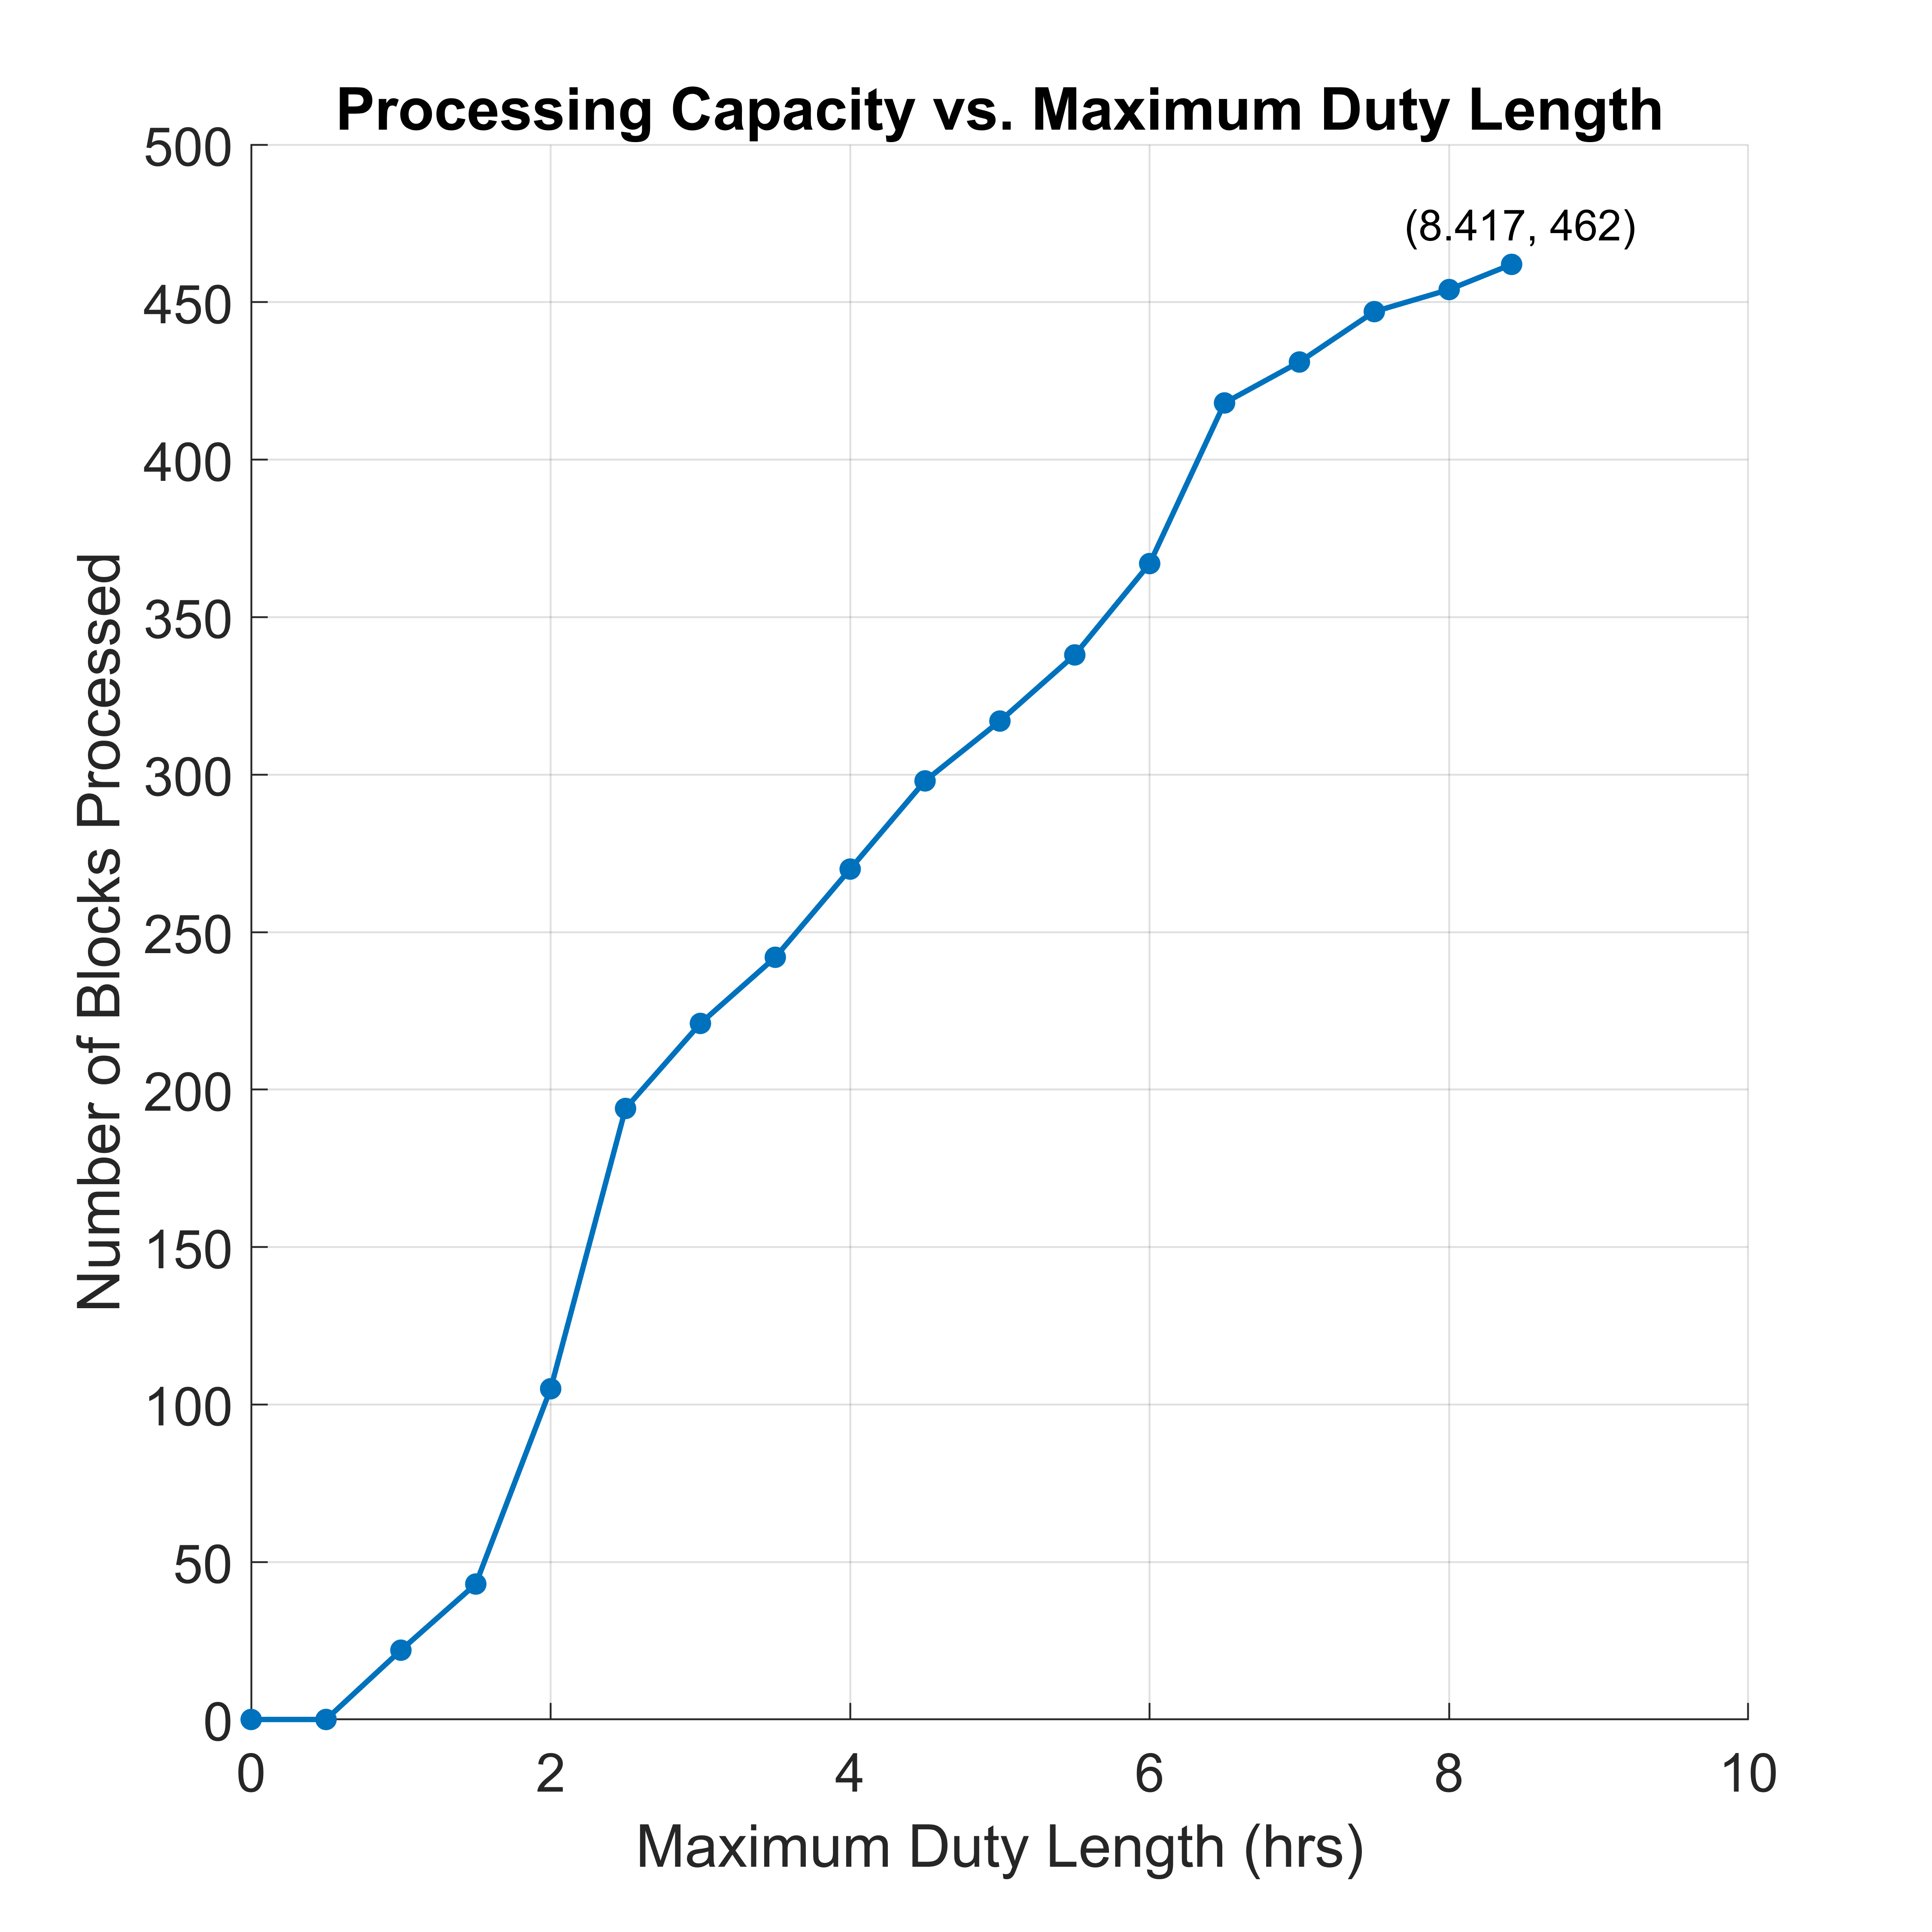
\includegraphics[width=0.46\linewidth]{[1] - chapter/Image Files/1-D1M3.png}
    \caption{Depicts the number of blocks that can be processed as a function of the Maximum Duty Length varied in 30 minute intervals, up to an \textit{upper threshold} that provides the first schedule that is feasible.}
    \label{fig:1-D1M3}
\end{figure}


%%%%%%%%%%%%%%%%%%%%%%%%%%%%%%%%%%%%%%%%%%%%%%%%%%%%%%%%%%%%%%%%%%%%%%%%%%%%%%% sub-SECTION %%%%%%%%%%%%%%%%%%%%%%%%%%%%%%%%%%%%%%%%%%%%%%%%%%%%%%%%%%%%%%%%%%%%%%%%%%%%%%

\subsection*{Evaluation}
Applying equation (\ref{equation: M3}) to the \textbf{historical} instance and by repeating this process in conjunction with the Pareto algorithm (\ref{alg: Pareto}) 18 times we receive the curve \ref{fig:1-D1M3} depicting the results of the sensitivity analysis. In the study of this problem we keep the amount of duties fixed to 183 available, and are only concerned with the effects on the processing capacity of the schedule (i.e. the amount of blocks that can fit in those duties).

\subsubsection*{Qualitative Results}
The trade-off curve shows the efficient frontier that we have created in its entirety. The frontier, shows us that as expected while we decrease the value of \textit{L} the schedules that we are able to create have an ever-decreasing processing capacity since as we can see they are able to process a continuously decreasing amount of blocks. The right end of the curve shows the only feasible schedule featured on this curve. That point with $L=8.417 \text{ hours}$ is the meeting point between the problem that we are currently solving and its symmetric that was studied in Section \ref{section:minimise duties}. The symmetry of the two problems is confirmed through this function since the schedule rightmost schedule of Figure \ref{fig:1-D1M3} coincides with the leftmost schedule of Figure \ref{fig:1-D1M2} since they both refer to schedules with 183 duties, 462 blocks processed and an $L=8.417 \text{ hours}$.

\subsubsection*{Quantitative Results}
Another interesting finding concerns the relationship between the degradation of the processing capacity as a function of \textit{L}. As we can see in Figure \ref{fig:1-D1M3} if we reduce the duty length by 2 hours, (\textbf{25\% reduction}), the decrease in duties that can be performed is only of the order of magnitude of \textbf{10\%}. This finding is in the direction of obtaining the trade-off relationship between finding the maximum duty length and the effect it has on the processing capacity of the MC. A practical understanding provided by this finding is that if we decrease \textit{L} by this 2 hour interval i.e. down to around 6 and a half hours, we will not have a proportional decrease in the processing capacity. From the perspective of Royal Mail, this insight could mean that we could allow a small portion of people to work part-time if they so wish. This insight is explained by the fact that this group of part-time employees could carry out that \textbf{10\%} of blocks that are left unscheduled. Moreover, since they would only work part-time they would work considerably less hours, hence allowing for the decrease seen in \textit{L} of the order of textbf{25\%}. These insights are not concrete proof that this would work for Royal Mail, but they show that significantly reducing drivers' work time results in a not so significant reduction in the number of blocks that can be processed.

\subsection*{Evaluation - Optimising Redefined Instance}

%%%%%%%%%%%%%%%%%%%%%%%%%%%%%%%%%%%%%%%%%%%%%%%%%%%%%%%%%%%%%%%%%%%%%%%%%%%%%%% Figure %%%%%%%%%%%%%%%%%%%%%%%%%%%%%%%%%%%%%%%%%%%%%%%%%%%%%%%%%%%%%%%%%%%%%%%%%%%%%%

\begin{figure}%
    \centering
    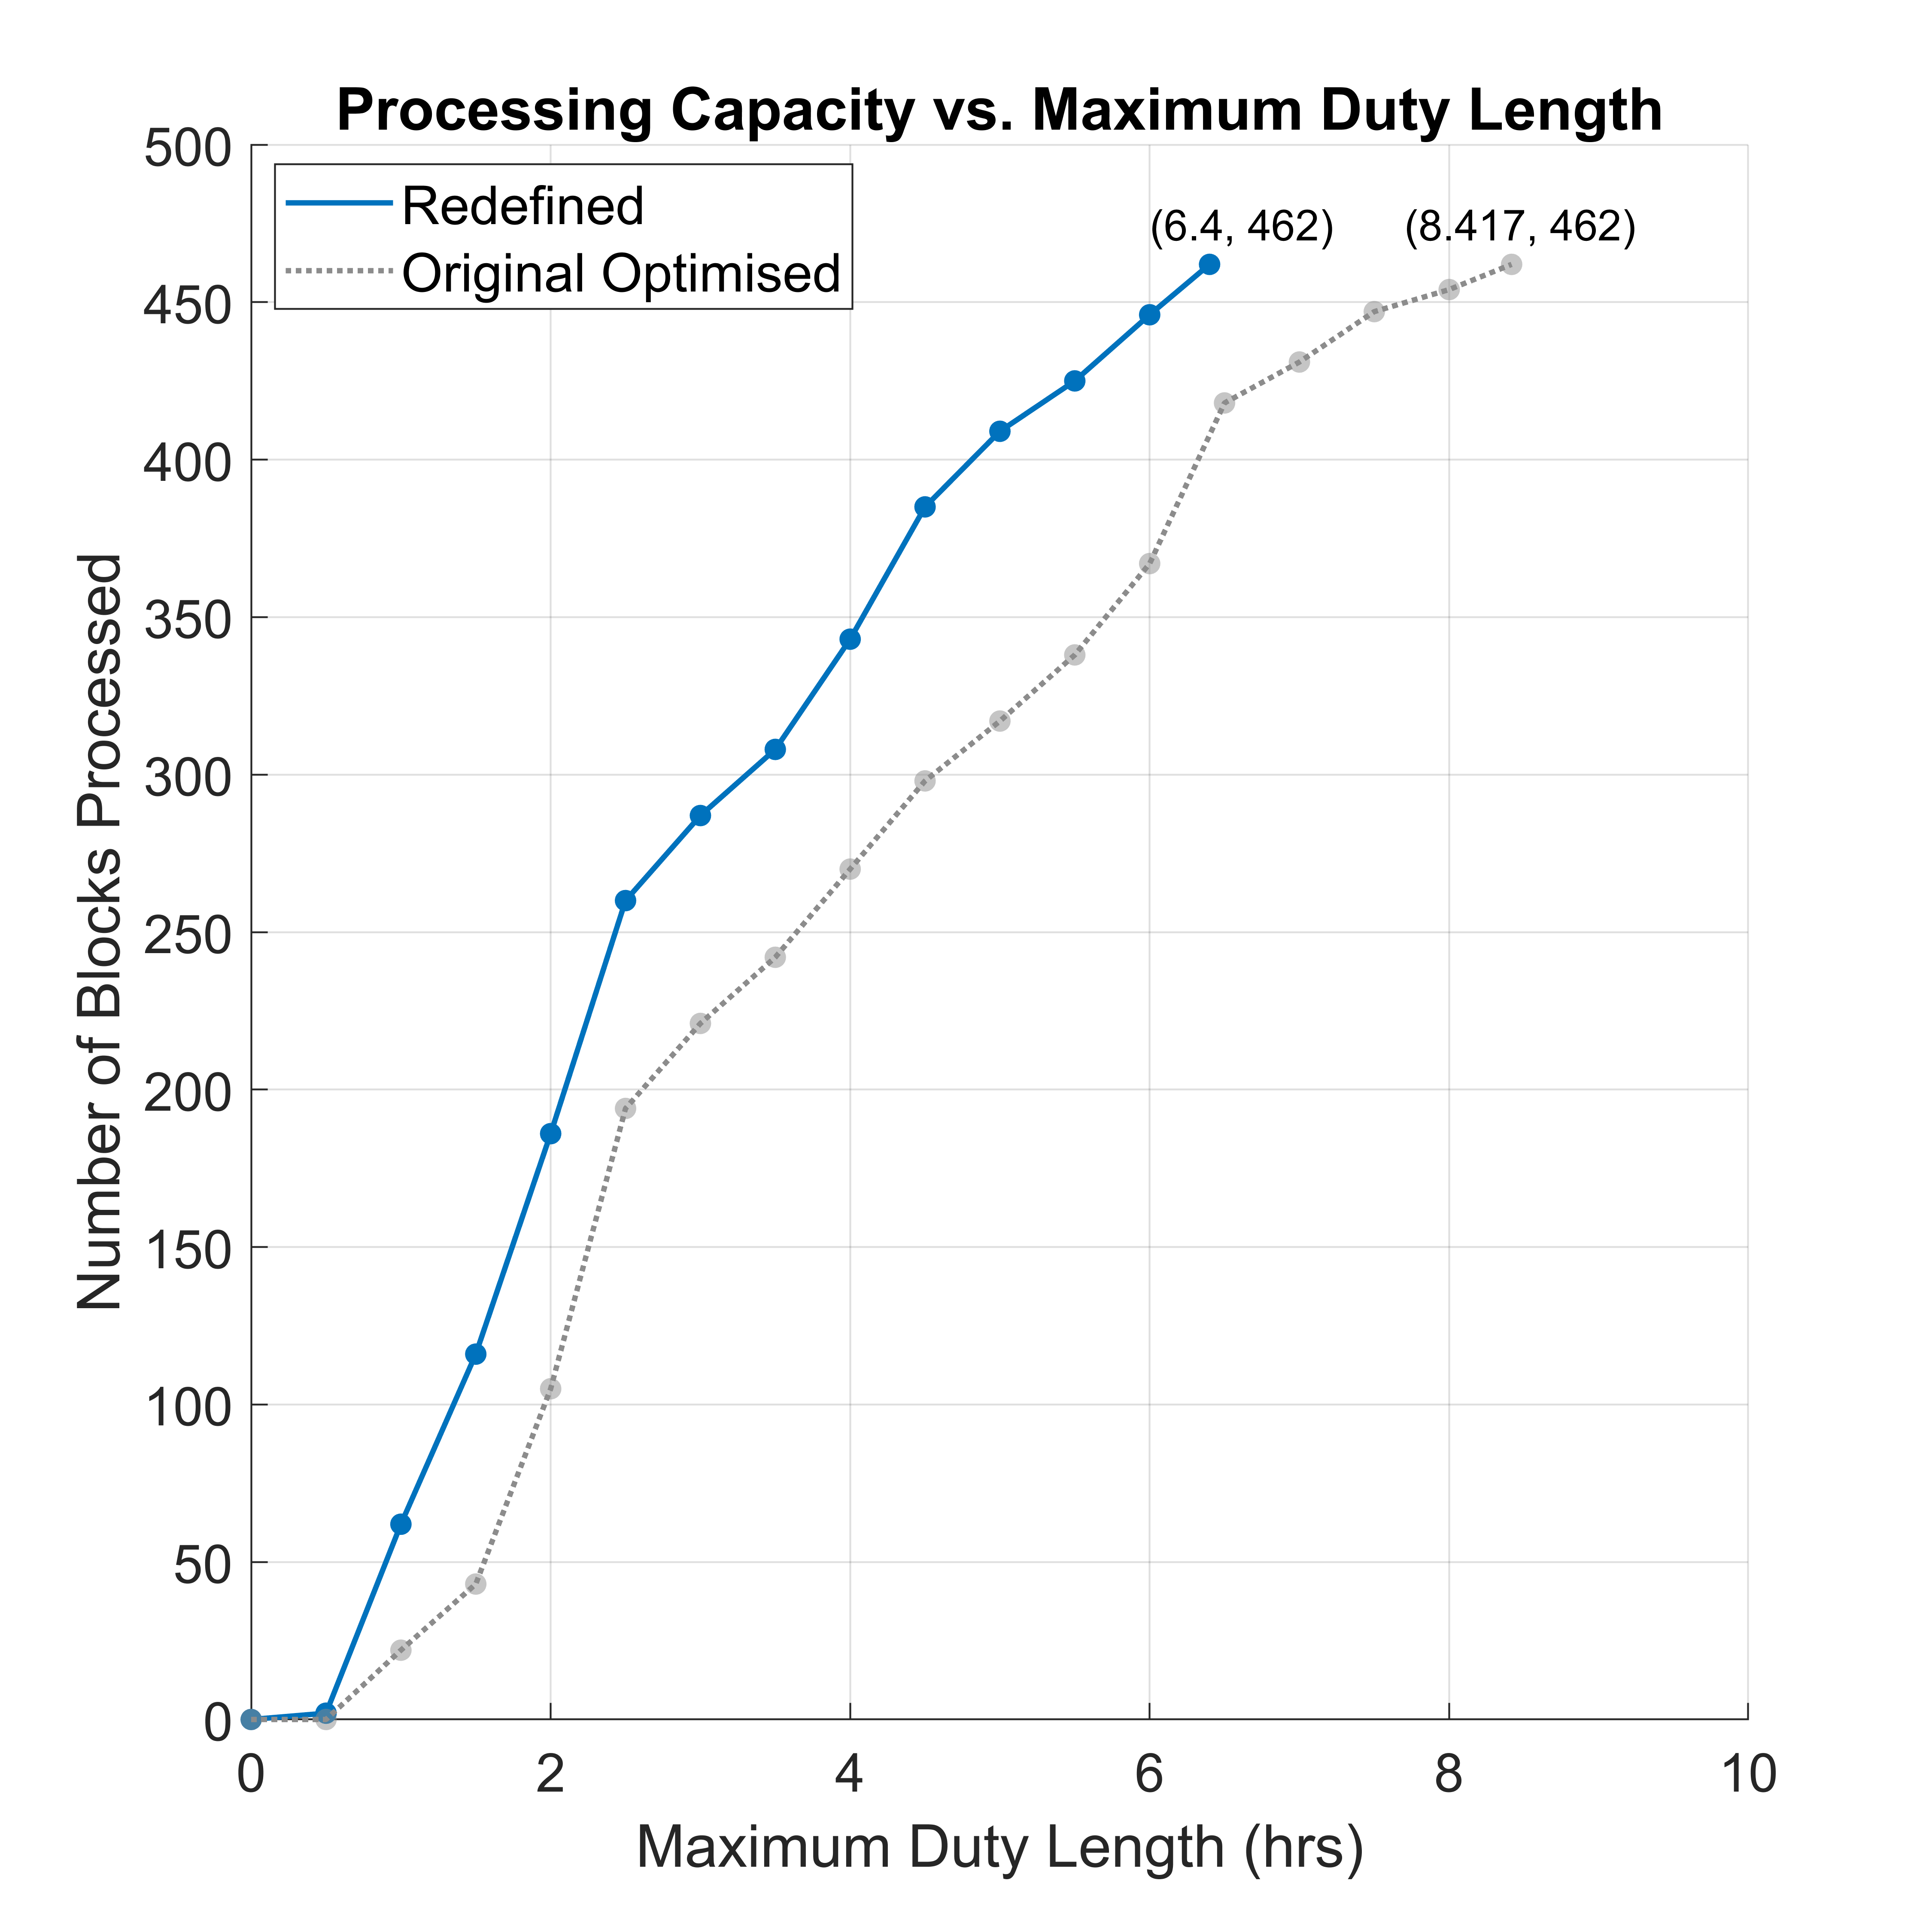
\includegraphics[width=0.46\linewidth]{[1] - chapter/Image Files/1-D2M3.png}
    \caption{Compares the number of blocks that can be processed as a function of the Maximum Duty Length for the Redefined and Historical instances.}
    \label{fig:1-D2M3}
\end{figure}

\vspace{\baselineskip}
\noindent
In a similar fashion to the case of the results from the Redefined instances in Section \ref{section:minimise duties}, the application of the Redefined instances provides marginally better results. In more detail, as seen in Figure \ref{fig:1-D2M3}, the processing capacity of the schedules generated based on the Redefined instances is hindered ever so slightly less, in comparison to the Historical instance's. That is an expected phenomenon, since as we mentioned before the blocks of the Redefined instances, contain naturally smaller blocks, since they do not consider the redundant activities. As a result, more of them can generally fit in the same 183 duties, which explains the smaller degradation in the processing capacity for the same level of \textit{L} compared to the Historical instance's schedules. 
%%%%%%%%%%%%%%%%%%%%%%%%%%%%%%%%%%%%%%%%%%%%%%%%%%%%%%%%%%%%%%%%%%%%%%%%%%%%%%% SECTION %%%%%%%%%%%%%%%%%%%%%%%%%%%%%%%%%%%%%%%%%%%%%%%%%%%%%%%%%%%%%%%%%%%%%%%%%%%%%%

\section{Load Balancing with Pre-emptions}
\label{section: Pre-emptive}
The final experiment run in this chapter involves the further investigation of the \textbf{theoretical optimal schedule} discussed in the final parts of the evaluations of the prior sections. In all three prior sections, we saw that there exists an absolute theoretical limit that would give us the corresponding \textbf{theoretical optimal schedule} with respect to the makespan objective. However, we also saw that the most optimal schedules that our solver was able to come up with would always have a certain optimality gap to that theoretical schedule. That theoretical schedule has been obtained through theoretically hypothesising that we can split the total schedulable labor hours equally in duties of equal length. Unlike, the other schedules discussed in this chapter it has not been obtain as an output from our solver. The purpose of exploring this topic is to investigate how close we can get to that theoretical limit with a schedule generated by our solver if we relax some of the design principles of our makespan formulation. 

\vspace{\baselineskip}
\noindent
It is normal to expect that completely achieving the theoretical limit is not a possibility. That is because as explained in the previous sections to obtain that theoretically optimal schedule we would have to completely disregard the structure of our components. Namely, we would have to discretise our activities and blocks with a very high frequency, effectively rendering them a collection of time instants that can exactly fit in duties of any length. However, that experiment is of little utility to us. In investigating how close we can get to approaching the theoretical limit, we choose to only breakdown the size of the blocks, but maintain the structure and processing times of the activities intact. Hence, we still expect not to be able to completely approach the theoretical limit, because cases where activities lengths' do not exactly fit in duties are expected to occur.  


\vspace{\baselineskip}
\noindent
To develop a schedule that approaches the theoretical limit we ran the MIP seen in Section \ref{section:Makespan Scheduling-content}, but by allowing the model to act \textbf{preemptively}. Non-pre-emptive formulations were used in all previous three models. By disregarding this design parameter we grant the model complete freedom in terms of the policy with which it can process each block. Effectively, we provide it with an additional degree of freedom that allows it to switch between blocks while processing one already. Effectively, it is allowed to process activities from different blocks even after having begun the processing of an activity from a different block. 

\vspace{\baselineskip}
\noindent
In practice, we carry this out by supplying instances of $I = \langle{m},\langle{B},A\rangle{}$ of the problem in an environment of $D=\{1,...,m\}$ parallel duties. However, in addition to a set of blocks we provide a set of activities $A =\{1,...,n\}$. The Historical instance utilised contained 3,285 activities that were allocated once again among a set of 183 duties. 

\vspace{\baselineskip}
\noindent
Through supplying activities as the component to be scheduled, the model is now \textbf{pre-emptive} with respect to blocks, since the solver is allowed to move activities around within each duty hence, breaking the original structure of the blocks. Consequently, we have allowed the model to switch between blocks by allowing it to start processing an activity from one block and then switch to processing an activity from a different block. The activities $j \in A$ all have their processing time $p_{j}$ as before. 

\vspace{\baselineskip}
\noindent
The \textit{MILP} is marginally changed. The biggest change is seen in the constraint: $\sum _{i=1}^m x_{i,j} = 1$ which is converted to $\sum _{i=1}^m x_{i,j} = p_j$ \cite{DUMMY:2}. Moreover $x_{i,j}$ are no longer binary variables. Variables $x_{i,j}$ now represent the time each block spends on each machine compared to whether machine \textit{i} executes job \textit{j} as before.

\vspace{\baselineskip}
\noindent
As a result formulation (\ref{equation: Makespan Scheduling}) from Section \ref{section:Makespan Scheduling-content} becomes:

%%%%%%%%%%%%%%%%%%%%%%%%%%%%%%%%%%%%%%%%%%%%%%%%%%%%%%%%%%%%%%%%%%%%%%%%%%%%%%% Maths %%%%%%%%%%%%%%%%%%%%%%%%%%%%%%%%%%%%%%%%%%%%%%%%%%%%%%%%%%%%%%%%%%%%%%%%%%%%%%

\vspace{\baselineskip}
\begin{equation}
\label{equation: Makespan preemptive}
\begin{aligned}
&\text{minimise}
%& & y_{i}  \\ %\todo{why y and and not yi}
& & y  \\ 
& \text{subject to}
% & & y_{i} = \sum _{j=1}^n x_{i,j}p_{j}  \;\;\; &\forall \; i \in D\tag{1}\\   
& & y\geq \sum _{j=1}^n x_{i,j}  \;\;\; &\forall \; i \in D\\   
& & &\sum _{i=1}^m x_{i,j} = p_j \;\;\; &\forall \; j \in B\\
& & &y \geq \sum _{i=1}^m x_{i,j}  \;\;\; &\forall \; j \in B\\
% & & &\sum _{j=1}^n x_{i,j}p_{j} \leq f_{i}-s_{i} \;\;\; &\forall \; i \in D\\ %{\color{red} we deleted the constraint that involves the length of duty being less than end-start.}
& & & y,x_{i,j}\geq 0  \\
\end{aligned}
\end{equation}

\vspace{\baselineskip}
\noindent
The problems objective is once again to minimise the \textbf{makespan} while obtaining a feasible schedule. The first constraint assigns $y$ its definition of the \textbf{makespan}, since the makespan must be greater or equal to the completion time of the longest lasting machine. With the second constraint we ensure that each job is performed to completion on the various machines that process it. The final constraint ensures that no block is processed for more total time than the makespan itself.

%%%%%%%%%%%%%%%%%%%%%%%%%%%%%%%%%%%%%%%%%%%%%%%%%%%%%%%%%%%%%%%%%%%%%%%%%%%%%%% sub-SECTION %%%%%%%%%%%%%%%%%%%%%%%%%%%%%%%%%%%%%%%%%%%%%%%%%%%%%%%%%%%%%%%%%%%%%%%%%%%%%%

\subsection*{Evaluation}
To investigate how close we can approach to the theoretical limit of the maximum duty length, we attempt through this experiment to establish a practical lower-bound solution. As mentioned in the beginning of this section, we do not expect to achieve the \texttt{absolute theoretical limit}. But by investigating the effects a preemptive model would have on our results, we can obtain a realisable best possible solution that we can hope to achieve. The \texttt{absolute theoretical limit} is that of a maximum duty length equal to the average duty length of the instance, which in the case of the Historical instance is equal to 7 hours and 50 minutes.

\vspace{\baselineskip}
\noindent
The results of the preemptive model hints to a lower-bound for the maximum duty length of 8 hours and 5 minutes. Compared to the makespan of 8 hours and 25 minutes this is a significant improvement in the maximum duty length. In fact this is a \textbf{7\%} improvement in the optimality gap with the \texttt{absolute theoretical limit}. 

%%%%%%%%%%%%%%%%%%%%%%%%%%%%%%%%%%%%%%%%%%%%%%%%%%%%%%%%%%%%%%%%%%%%%%%%%%%%%%% sub-SECTION %%%%%%%%%%%%%%%%%%%%%%%%%%%%%%%%%%%%%%%%%%%%%%%%%%%%%%%%%%%%%%%%%%%%%%%%%%%%%%

\subsection*{Evaluation - Optimising Redefined Instance}
We repeat the process outlined above to calculate the effect of pre-emption on the Redefined instance. We ran the MILP (\ref{equation: Makespan preemptive}) but with an instance containing 2,850 activities that were once again allocated among a set of 183 duties. The \texttt{absolute theoretical limit} in this case would be to obtain a schedule where \textit{L} would be equal to the average duty length of the instance (i.e. 06:06). 

\vspace{\baselineskip}
\noindent
Upon running the pre-emptive model on the instance we obtain a practical lower-bound of 6 hours and 32 minutes. Similar to the prior case of the Historical instance this is a significant improvement over the previously obtained makespan of 7 hours and 27 minutes. In quantitative terms this is a bigger improvement compared to the Historical instance's case, of magnitude \textbf{23\%}.
\chapter{Dealing with Uncertainty} 
\label{chapter:Benchmark Instances}

%%%%%%%%%%%%%%%%%%%%%%%%%%%%%%%%%%%%%%%%%%%%%%%%%%%%%%%%%%%%%%%%%%%%%% Section %%%%%%%%%%%%%%%%%%%%%%%%%%%%%%%%%%%%%%%%%%%%%%%

Following an initial analysis of the historical schedules and the discovery of significant room for optimisation, we now study the effects that the addition of an \textbf{uncertainty component} will have on our schedules.

\vspace{\baselineskip}
\noindent
The chapter begins by outlining the reasoning behind our wish to examine the concept of uncertainty. Section \ref{section: Generating Uncertainty} begins the study by discussing the procedures followed to generate the uncertainty components. Section \ref{section: effect of uncertainty} continues that discussion by analysing the effect the uncertainty components have on our previously optimally generated schedules. It focuses on the robustness of those optimal schedules. Finally, Section \ref{section: Methodologies} studies two new methodologies that will hopefully enhance the robustness of our proposed schedule, and compares every optimal schedule that we have generated to determine the most robust, with respect to the uncertainty components.

%%%%%%%%%%%%%%%%%%%%%%%%%%%%%%%%%%%%%%%%%%%%%%%%%%%%%%%%%%%%%%%%%%%%%% Section %%%%%%%%%%%%%%%%%%%%%%%%%%%%%%%%%%%%%%%%%%%%%%%

\vspace{\baselineskip}
\noindent
 Our study on uncertainty begins by considering the optimal schedule from the Makespan Scheduling Section \ref{section:Makespan Scheduling-content} of Chapter \ref{chapter: 2-Evaluating Royal Mail Historical Data}. In particular, henceforth we call the \textbf{Makespan optimised} schedule from the Historical dataset our \textbf{nominal} instance. In essence, it represents what we would like to take place at the MC for the majority of the time. However, for the purposes of this uncertainty study we want to investigate the degree to which this optimal schedule is \textbf{robust} with respect to various degrees of \textbf{uncertainty}. The purpose of studying this, is to ensure that the schedules generated from our optimisation models will withstand random perturbations that simulate what might occur on a given day at Royal Mail. We argue that robustness of a schedule is dependent upon two optimality criteria. When comparing two schedules, we can characterise as more robust the schedule that achieves the lowest makespan value \cite{DBLP:approximatingbounded} or the least amount of duties that end up overrunning a maximum duty threshold, defined below. In cases that one schedule performs better in one of the criteria and the other outperforms it in the other criterion, it is left to the scheduler's judgement to determine which schedule is more robust depending on the magnitude of the out-performance in the respective criterion.

%%%%%%%%%%%%%%%%%%%%%%%%%%%%%%%%%%%%%%%%%%%%%%%%%%%%%%%%%%%%%%%%%%%%%% Figure %%%%%%%%%%%%%%%%%%%%%%%%%%%%%%%%%%%%%%%%%%%%%%%

\begin{figure}
    \centering
    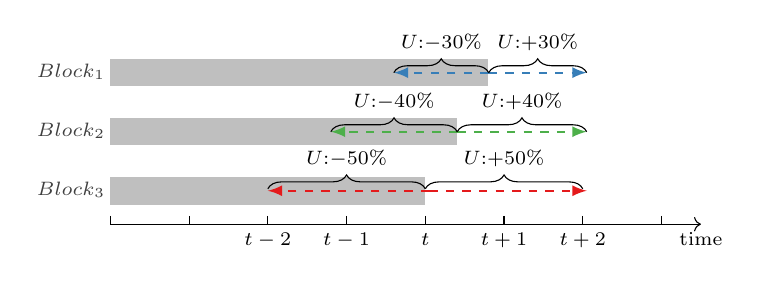
\begin{tikzpicture}[%
        every node/.style={
            font=\scriptsize,
            % Better alignment, see https://tex.stackexchange.com/questions/315075
            text height=1ex,
            text depth=.25ex,
        },
    ]
    % draw horizontal line   
    \draw[->] (1,0) -- (8.5,0);
    
    % draw vertical lines
    \foreach \x in {1,...,8}{
        \draw (\x cm,3pt) -- (\x cm,0pt);
    }
    
    % place axis labels
    \node[anchor=north] at (3,0) {$t-2$};
    \node[anchor=north] at (4,0) {$t-1$};
    \node[anchor=north] at (5,0) {$t$};
    \node[anchor=north] at (6,0) {$t+1$};
    \node[anchor=north] at (7,0) {$t+2$};
    \node[anchor=north] at (8.5,0) {time};
    
    % Bar for Block1
    %\draw[fill=myLightGray] (1,0.25) rectangle (2,0.6);
    \fill[myLightGray] (1,0.25) rectangle (2,0.6);
    \fill[myLightGray] (2,0.25) rectangle (3,0.6);
    \fill[myLightGray] (3,0.25) rectangle (4,0.6);
    \fill[myLightGray] (4,0.25) rectangle (5,0.6);
    \draw[myRed,dashed,thick,-latex] (5.05,0.425) -- (7.05,0.425);
    \draw[myRed,dashed,thick,-latex] (5.05,0.425) -- (3,0.425);
    
    % Bar for Block2
    \fill[myLightGray] (1,1) rectangle (3,1.35);
    \fill[myLightGray] (3,1) rectangle (4,1.35);
    \fill[myLightGray] (4,1) rectangle (5,1.35);
    \fill[myLightGray] (5,1) rectangle (5.4,1.35);
    \draw[myGreen,dashed,thick,-latex] (5.405,1.175) -- (7.05,1.175);
    \draw[myGreen,dashed,thick,-latex] (5.405,1.175) -- (3.8,1.175);
    
    % Bar for Block3
    \fill[myLightGray] (1,1.75) rectangle (3,2.1);
    \fill[myLightGray] (3,1.75) rectangle (4,2.1);
    \fill[myLightGray] (4,1.75) rectangle (5,2.1);
    \fill[myLightGray] (5,1.75) rectangle (5.8,2.1);
    \draw[myBlue,dashed,thick,-latex] (5.805,1.925) -- (7.05,1.925);
    \draw[myBlue,dashed,thick,-latex] (5.805,1.925) -- (4.6,1.925);
    
    % draw curly braces and add their labels
    \draw[decorate,decoration={brace,amplitude=5pt}] (3,0.45) -- (5,0.45)
        node[anchor=south,midway,above=4pt] {$U$:$-$50\%};
    \draw[decorate,decoration={brace,amplitude=5pt}] (5,0.45) -- (7,0.45)
        node[anchor=south,midway,above=4pt] {$U$:$+$50\%};  
        
    \draw[decorate,decoration={brace,amplitude=5pt}] (3.8,1.175) -- (5.405,1.175)
        node[anchor=south,midway,above=4pt] {$U$:$-$40\%};
    \draw[decorate,decoration={brace,amplitude=5pt}] (5.405,1.175) -- (7.05,1.175)
        node[anchor=south,midway,above=4pt] {$U$:$+$40\%};   
        
    \draw[decorate,decoration={brace,amplitude=5pt}] (4.6,1.925) -- (5.805,1.925) 
        node[anchor=south,midway,above=4pt] {$U$:$-$30\%};
    \draw[decorate,decoration={brace,amplitude=5pt}] (5.805,1.925)  -- (7.05,1.925)
        node[anchor=south,midway,above=4pt] {$U$:$+$30\%};       
        
    % Place the label inside block:
    \node [darkgray] at (+0.5,0.425) {$Block_3$};
    \node [darkgray] at (+0.5,1.175) {$Block_2$};
    \node [darkgray] at (+0.5,1.925) {$Block_1$};
    %\node [centre,darkgray] at (+6,0.7) {};
    %\node [centre,darkgray] at (+4,0.7) {};
    
    \end{tikzpicture}
    \caption{The effect of the application of box uncertainty sets of different magnitudes on the duration of blocks.}
    \label{fig:Generating Uncertainty}
\end{figure}

\section{Uncertainty Generation}
\label{section: Generating Uncertainty}
We generate \textit{disturbed} instances by using the nominal instance as our foundation, to which we then apply uncertainty components of various magnitudes. The uncertainty components are applied onto each schedule's blocks, which we subsequently will attempt to fit inside the duties. We begin by applying \textbf{box uncertainty sets} of magnitudes $U:$ $\pm30\%$,$\pm40\%$,$\pm50\%$ respectively. As seen for example on Figure \ref{fig:Generating Uncertainty}, when we apply an uncertainty component of magnitude $U$: $\pm30\%$, each block's \textit{processing time} $p_j$ can randomly \textbf{shrink} or \textbf{expand} by up to a maximum of 30\%, equivalently for uncertainty sets of other magnitudes. 

\todo{add a thing like schedule apply uncertainty recovered}

\vspace{\baselineskip}
\noindent
In generating the first set of samples, we created ten disturbed instances per uncertainty set, a total of 30. We chose to showcase the \textbf{most disturbed} instances in Table \ref{table:Applying Uncertainty Set on Nominal}. We measure the disturbance of the uncertainty set on the instance by examining the degree to which the \texttt{Total Time} of the instance has increased or decreased. Hence, for each uncertainty set we present the two instances for which we observed the largest increase, and decrease of the \texttt{Total Time} away from the nominal instance's \texttt{Total Time} benchmark. We henceforth refer to each group as \texttt{reduced} and \texttt{augmented}, for reduced and increased \textit{Total time} respectively \cite{DBLP:journals/corr/abs-1805-03437}. 

\vspace{\baselineskip}
\noindent
The thought process behind choosing the most disturbed instances per uncertainty set, is based on the idea that less disturbed instances will achieve levels of performance in between these two extremes when optimised, hence we can approximate their performance by using those two boundary cases for our analysis. 

%%%%%%%%%%%%%%%%%%%%%%%%%%%%%%%%%%%%%%%%%%%%%%%%%%%%%%%%%%%%%%%%%%%%%%%%%%%%%%% Table %%%%%%%%%%%%%%%%%%%%%%%%%%%%%%%%%%%%%%%%%%%%%%%%%%%%%%%%%%%%%%%%%%%%%%%%%%%%%%

\begin{table}[t]
\small
    \centering 
    \begin{tabular}{|c|c|c|c|c|}
        \hline
        \textbf{Instance} & \textbf{Total Time} & \multicolumn{3}{|c|}{ \textbf{Atomic Blocks} \textbf{(}$\pmb{p_j}$\textbf{)}} \\
        \hline
         \multicolumn{2}{|c|}{ }  & \texttt{Average} &  \texttt{Minimum} & \texttt{Maximum} \\
        \hline
        Nominal & 1,435:22  & 03:05 & 00:40 & 08:25 \\
        \hline
        \multirow{2}{*}{$U$: $\pm30\%$} & 1,416:36 & 03:03 & 00:30 & 10:00 \\
        \cline{2-5}
         & 1,446:14 & 03:07 & 00:29 & 10:12  \\
        \hline
        \multirow{2}{*}{$U$: $\pm40\%$} & 1,406:34 & 03:02 & 00:30 & 10:55  \\
        \cline{2-5}
         & 1,439:28 & 03:06 & 00:32 & 11:26 \\
        \hline
        \multirow{2}{*}{$U$: $\pm50\%$} & 1,391:17 & 03:00 & 00:23 & 10:44  \\
        \cline{2-5}
         & 1,454:18 & 03:08 & 00:20 & 10:52  \\
        \hline
    \end{tabular}%
    \medbreak
    \caption{Table showing the overall labor time and other characteristic values of atomic blocks from the two \textbf{most disturbed} (\texttt{reduced}, \texttt{augmented}) instances for each uncertainty set in (HH:mm).}
    \label{table:Applying Uncertainty Set on Nominal}
\end{table}

%%%%%%%%%%%%%%%%%%%%%%%%%%%%%%%%%%%%%%%%%%%%%%%%%%%%%%%%%%%%%%%%%%%%%% sub-Section %%%%%%%%%%%%%%%%%%%%%%%%%%%%%%%%%%%%%%%%%%%%%%%

\subsection*{Analysis of the Generated Instances}
\label{subsection: Analysis of  Disturbed Instances}
It is evident in Table \ref{table:Applying Uncertainty Set on Nominal} that the application of the uncertainty components will likely decrease the optimal nature of the nominal schedule, with respect to the makespan. This can be deduced from the fact that the nominal instance contains around 1,435 labour hours whereas in some cases the perturbed instances end up having to schedule more labour hours. By definition the more time that requires scheduling means the tougher for the optimisation solver to fit all blocks in a schedule with a reduced makespan. Hence, this first observation already hints to schedules with generally increased makespans for the disturbed instances. 

\vspace{\baselineskip}
\noindent
Moreover, as the magnitude of the uncertainty set is increased, we can see that the extremities as far as the durations of the blocks tend to increase accordingly. The increase in the duration of the longest lasting blocks will most likely result in a less robust schedule. Assuming our disturbed instance is \textbf{maximally disturbed} as those in Table \ref{table:Applying Uncertainty Set on Nominal}, we can see that there exist blocks that have a \textit{processing time} $p_j$ that surpasses the maximum $p_j$ observed in the nominal instance. As we saw in Section \ref{section:Makespan Scheduling-content} the maximum $p_j$ of 08:25 in the nominal instance also coincides with the nominal schedule's \textit{makespan}. Hence, the disturbed blocks with \texttt{Maximum} ($p_j$)\footnote{Observed in the final column of Table \ref{table:Applying Uncertainty Set on Nominal}} have durations larger than the nominal instance's makespan. Consequently, it is inevitable, even if the solver encloses only those particular blocks by themselves in one duty, to expect an increased makespan for the disturbed instances over the nominal instance. 

\vspace{\baselineskip}
\noindent
On the contrary, looking at the other end of the spectrum we can see that the \texttt{Minimum} ($p_j$) involves blocks with reduced \textit{processing times}. The blocks with shorter lasting durations are potentially going to be helpful in ensuring the uniformity of the optimised schedule since the solver can utilise them as a final buffer to be used in filling any non-utilised idle time at the end of a duty. In simple terms, the blocks with minimal processing times allow the solver greater flexibility in putting the duties together.

%%%%%%%%%%%%%%%%%%%%%%%%%%%%%%%%%%%%%%%%%%%%%%%%%%%%%%%%%%%%%%%%%%%%%% Section %%%%%%%%%%%%%%%%%%%%%%%%%%%%%%%%%%%%%%%%%%%%%%%

\section{Evaluating the Effect of Uncertainty}
\label{section: effect of uncertainty}
Having generated this new set of instances of the problem, our goal is to detect the effects theses various \textbf{degrees of uncertainty} have on the optimality of the nominal instance. We hypothesise that there exists a maximum duty threshold \textit{L} of 8 hours and 25 minutes, that should ideally not be exceeded by any duty under the application of uncertainty. Choosing the two most disturbed instances of Table \ref{table:Applying Uncertainty Set on Nominal} for each uncertainty set, we would like to measure the degree to which the optimised nominal schedule with makespan equal to \textit{L}, is \textbf{disturbed} for each set. The degree of the disturbance is evaluated by measuring the number of duties that overrun this \textit{L} plus a 15 minute interval, i.e. a \textbf{delay of a quarter of an hour}. We refer to this length of time as \textit{L'}. The purpose of this experiment is to gain an insight into the level of robustness of the nominal schedule, with respect to uncertainty. We pass each instance $D$ to the optimisation solver and by applying the \textbf{Makespan Scheduling} formulation of Section \ref{section:Makespan Scheduling-content}, we observe the effects in Table \ref{table:Uncertainty Schedules} and Figure \ref{fig: Uncertainty Sets Effects.}.

%%%%%%%%%%%%%%%%%%%%%%%%%%%%%%%%%%%%%%%%%%%%%%%%%%%%%%% Double Figure %%%%%%%%%%%%%%%%%%%%%%%%%%%%%%%%%%%%%%%%%%%%%%%%%%%%%%%%%%%%%%%%%%%%%%%%%%%

\begin{figure}%
    \centering
    \subfloat[Maximally disturbed instances with a \textbf{decrease} in overall labor time (\texttt{reduced}).]{%\begin{center}
    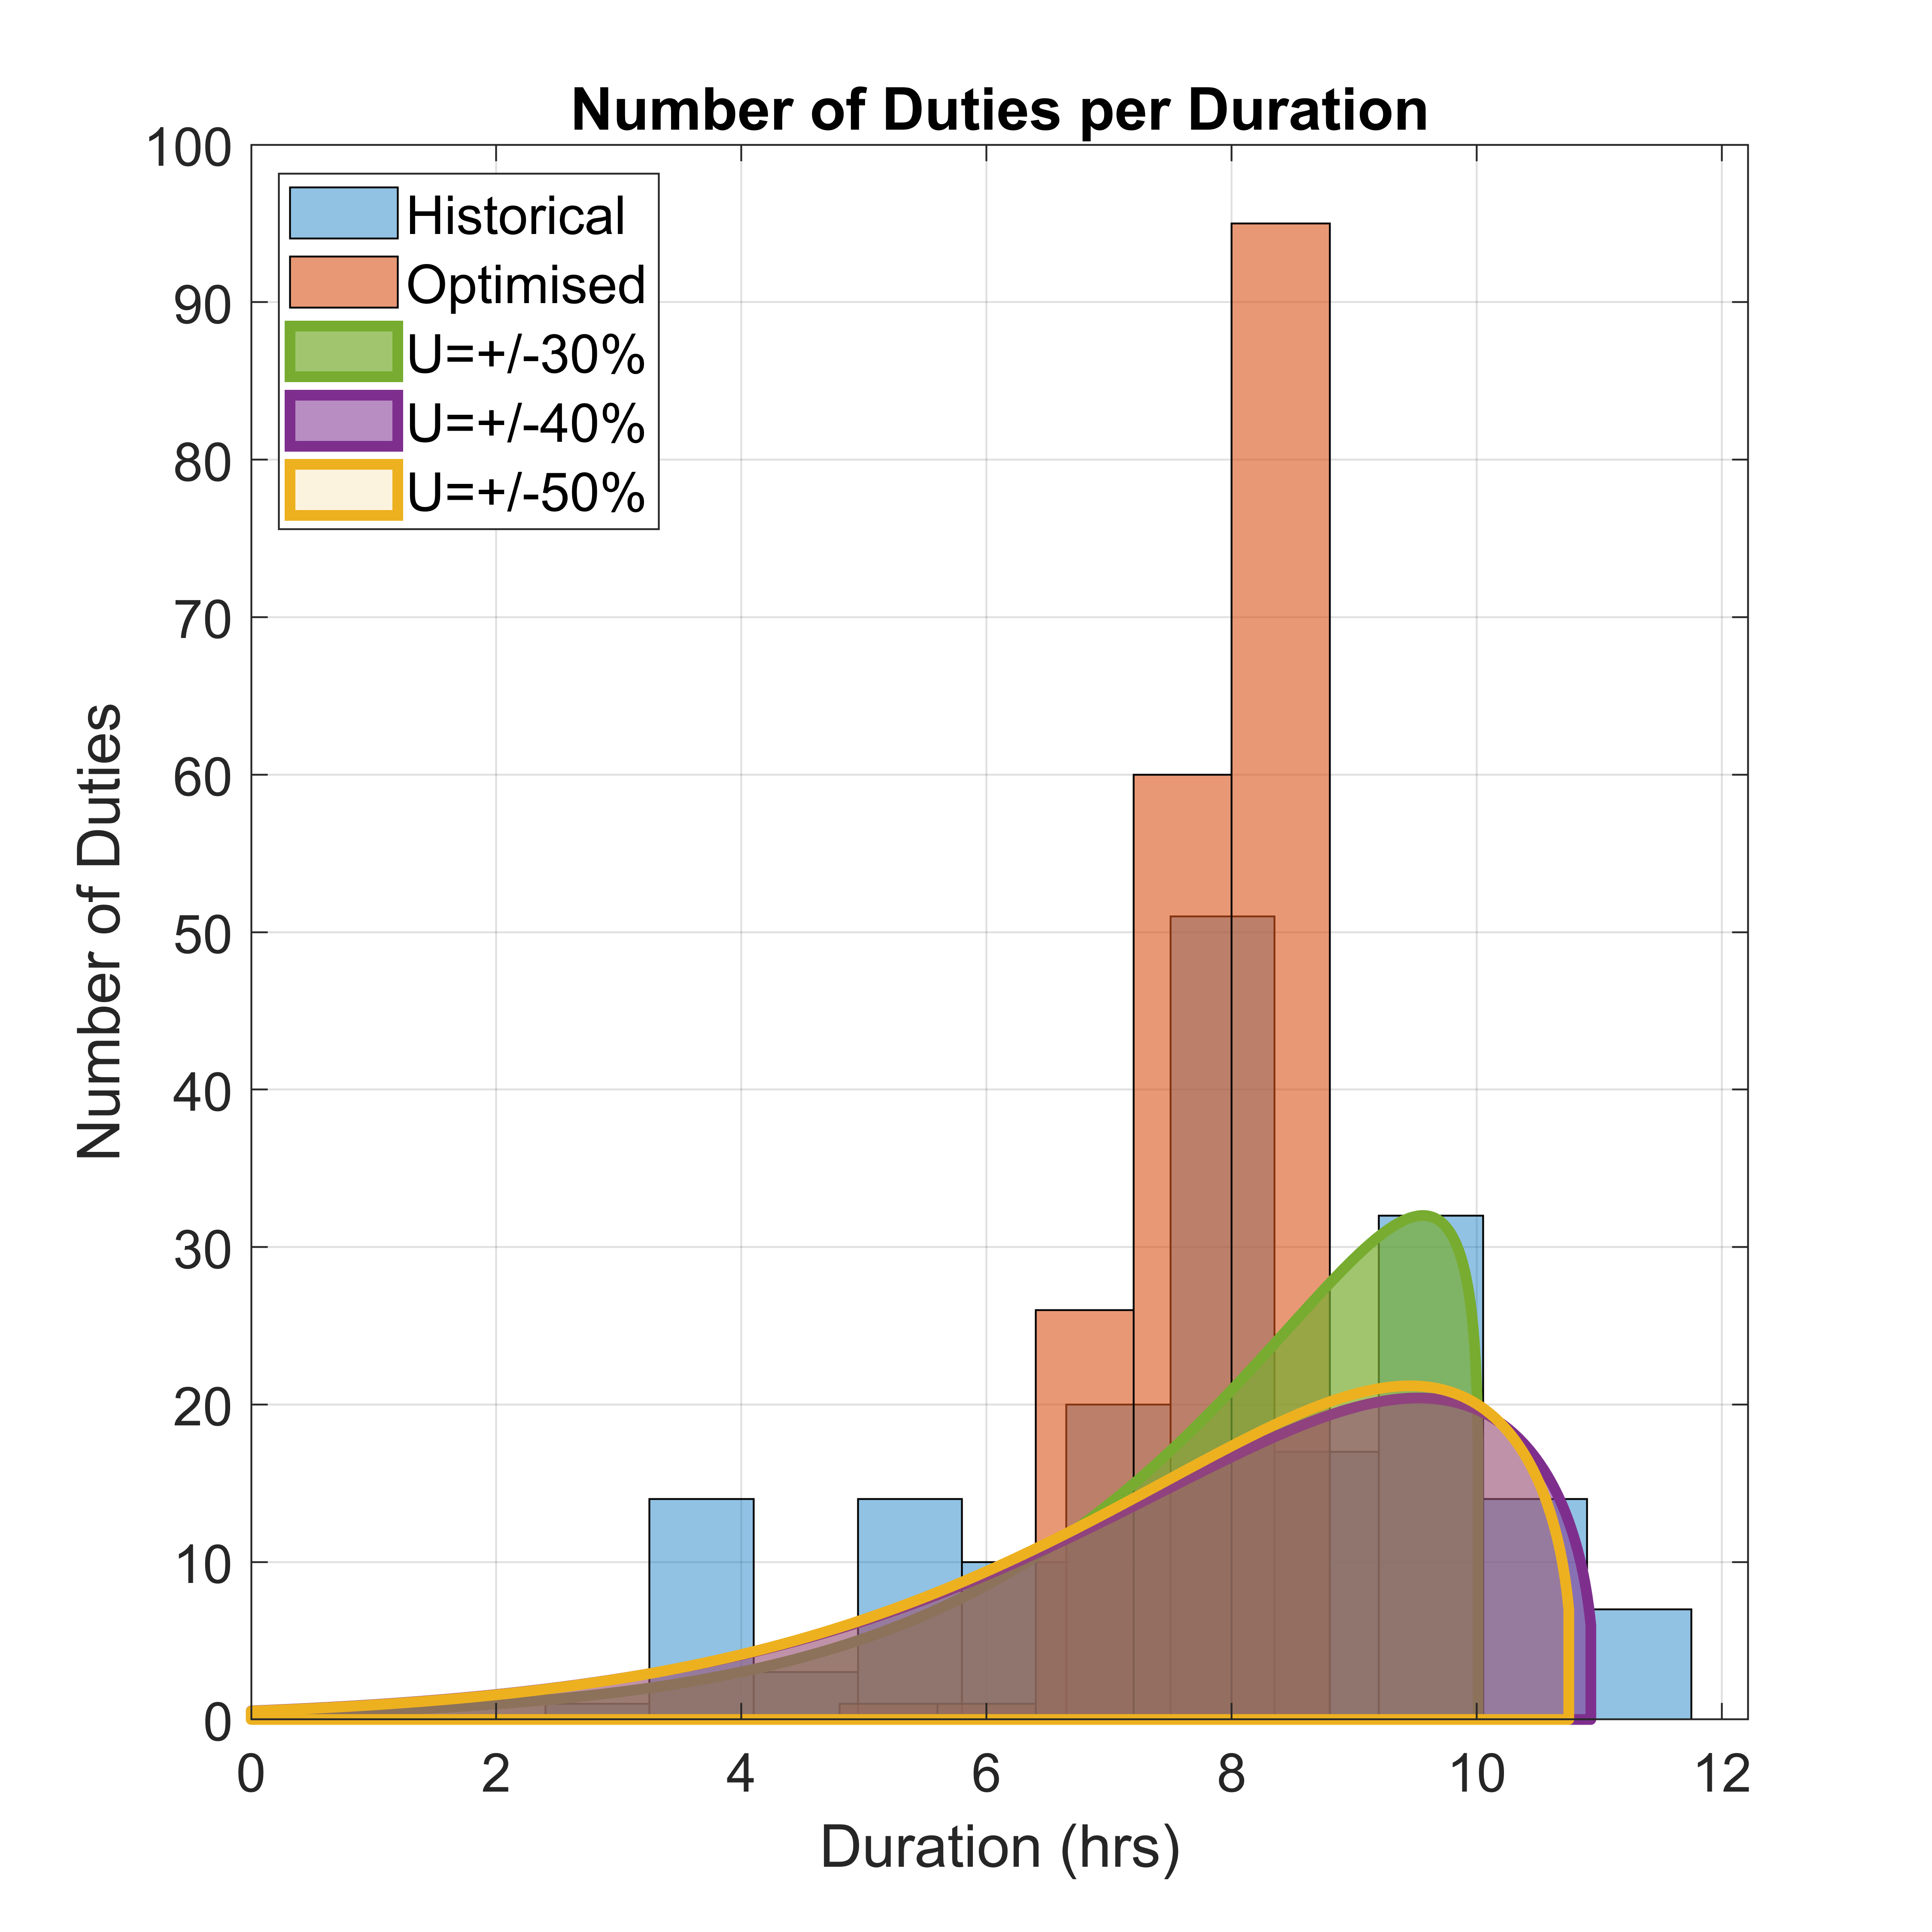
\includegraphics[width=0.46\linewidth]{[3] - chapter/Comparison_Of_Uncertainty_Sets_min.png}
    }%\end{center}}%end of picture #2
    \qquad
    %picture #2
    \centering
    \subfloat[Maximally disturbed instances with an \textbf{increase} in overall labor time (\texttt{augmented}).]{%\begin{center}
    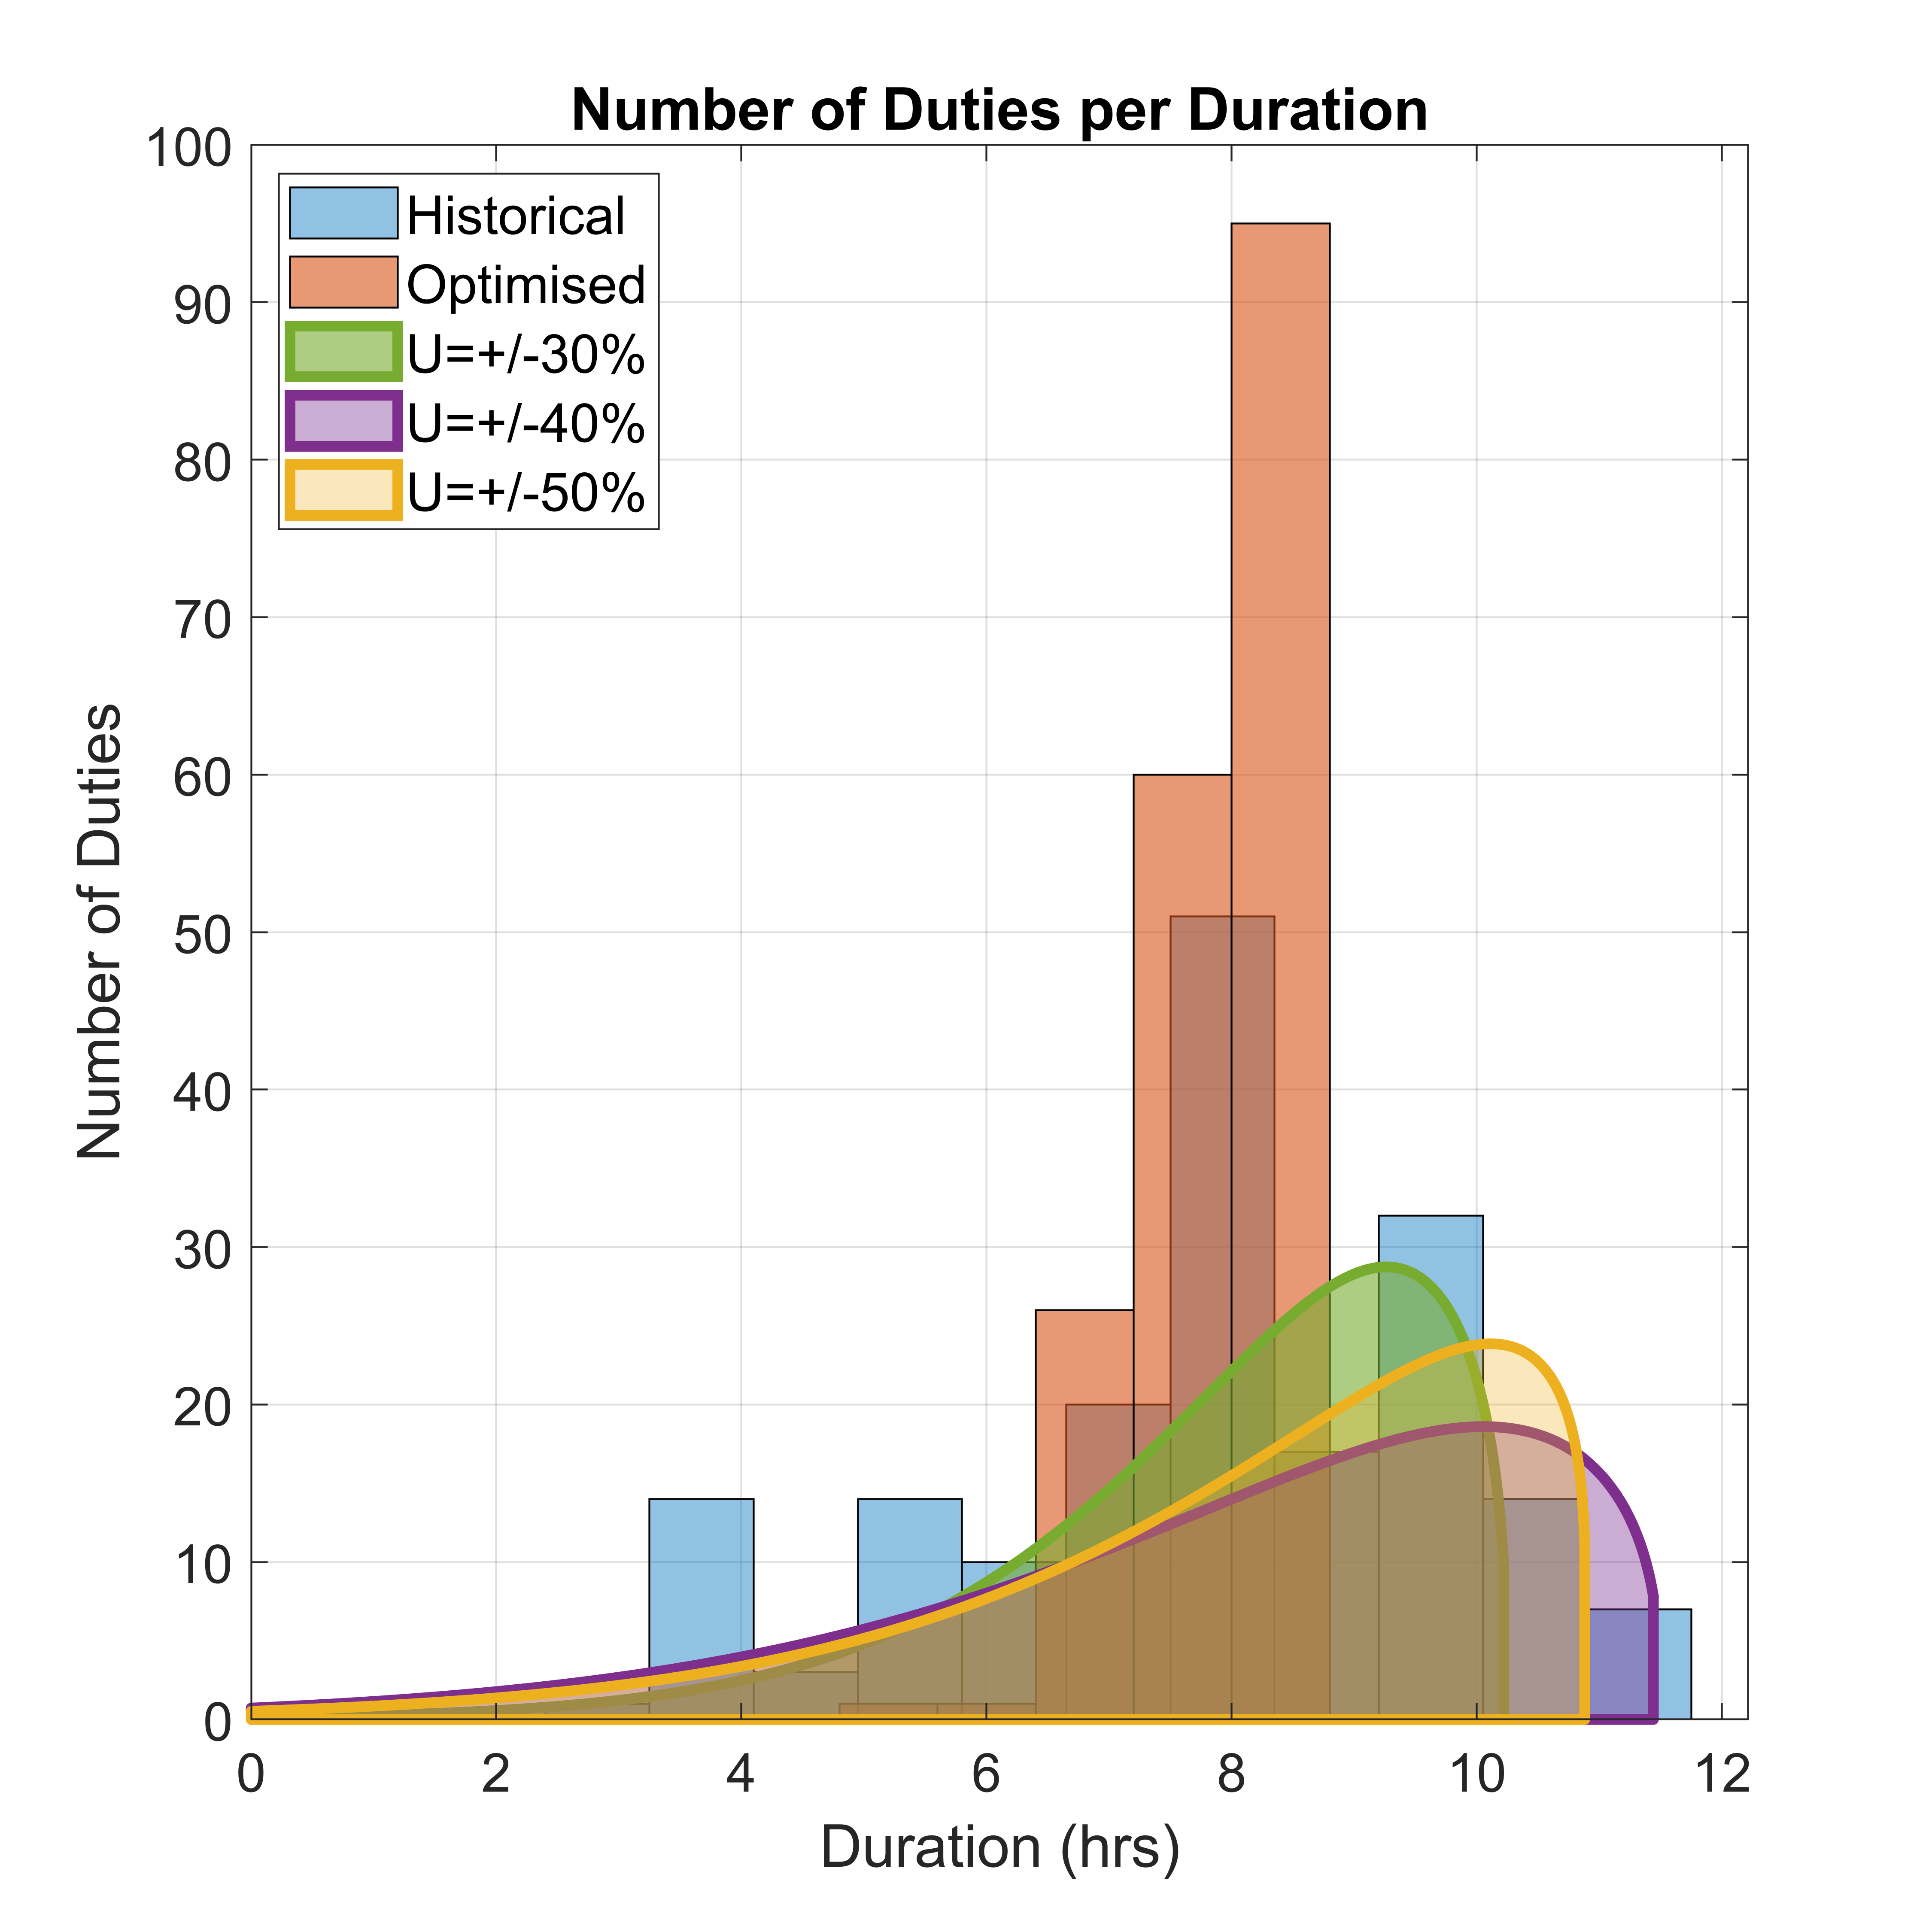
\includegraphics[width=0.46\linewidth]{[3] - chapter/Comparison_Of_Uncertainty_Sets_max.png}
    }%\end{center}}%picture #1
    \caption{The histograms provide an overview of the effects of various levels of uncertainty set on $Duty$ lengths.}
    \label{fig: Uncertainty Sets Effects.}
\end{figure}

%%%%%%%%%%%%%%%%%%%%%%%%%%%%%%%%%%%%%%%%%%%%%%%%%%%%%%%%%%%%%%%%%%%%%% Table %%%%%%%%%%%%%%%%%%%%%%%%%%%%%%%%%%%%%%%%%%%%%%%

\begin{table}[b]
\small
    \centering 
    \begin{tabular}{|c|c|c|c|c|}
        \hline
        \textbf{Schedule} & \textbf{Total Time} & \multicolumn{3}{|c|}{ \textbf{Duties (HH:mm)}} \\
        \hline
        \multicolumn{2}{|c|}{ }  & \texttt{Makespan} & \texttt{Minimum} & \texttt{Average}  \\
        \hline
        Historical & 1,435:22 & 11:45 & 02:50 & 07:50 \\
        \hline
        Nominal & 1,435:22 & 08:25 & 05:15 & 07:50 \\
        \hline
        \multirow{2}{*}{$U$: $\pm30\%$} &1,416:36 & 10:00 & 01:15 & 07:44 \\
        \cline{2-5}
         & 1,446:14 & 10:12 & 00:00 & 07:54  \\
        \hline
        \multirow{2}{*}{$U$: $\pm40\%$} & 1,406:34 & 10:44 & 00:00 & 07:40  \\
        \cline{2-5}
         & 1,439:28 & 11:26 & 00:00 & 07:51 \\
        \hline
        \multirow{2}{*}{$U$: $\pm50\%$} & 1,391:17 & 10:44 & 00:00 & 07:36  \\
        \cline{2-5}
         & 1,454:18 & 10:52 & 00:00 & 07:56  \\
        \hline
    \end{tabular}%
    \medbreak
    \caption{Table showing the duty characteristics and overall time scheduled of the Historical, Nominal and Disturbed Schedules.}
    \label{table:Uncertainty Schedules}
\end{table}

%\todo{make sure that number of duties epi avg duty = total hours}

\vspace{\baselineskip}
\noindent
In the figures we can see the Historical Schedule currently run by Royal Mail, as well as the nominal and disturbed instances with optimal Makespans. The effects of the application of the uncertainty components are somewhat unsurprising, given our expectations from the analysis of Section \ref{subsection: Analysis of  Disturbed Instances}. The optimal schedules of the disturbed instances are \textbf{less optimal} than the nominal, with respect to both their \textbf{makespan} and their \textbf{uniformity}. The makespans of the disturbed schedules that are also listed in Table \ref{table:Uncertainty Schedules} clearly show that the disturbed instances have longer lasting makespans and hence perform sub-par compared to the nominal instance. As mentioned, in Section \ref{subsection: Analysis of  Disturbed Instances} this a completely expected result since the makespans for all disturbed schedules are equal to their longest lasting block, hence it is the \texttt{Maximum} ($p_j$) that is the determining factor for the makespan. As was predicted the degree of the disturbance to the makespan increases roughly as a function of the magnitude of the uncertainty set applied. Perhaps the most interesting observation, however, is that we can see that the schedules with a $U$: $\pm40\%$ perturbation performs slightly worse than those with $U$: $\pm50\%$ in both cases.

\vspace{\baselineskip}
\noindent
In a similar fashion, the uniformity of the schedules is worsened as we increase the magnitude of the uncertainty set applied. This can be seen qualitatively in Figure \ref{fig: Uncertainty Sets Effects.}, since the bandwidths of the disturbed instances' distributions are considerably larger than both the historical and nominal's. As is evident the uniformity of the disturbed schedules is tied to the magnitude of uncertainty applied to them, once more noting that somewhat unexpectedly the $U$: $\pm40\%$ schedule is even less balanced than the $U$: $\pm50\%$, as determined by its larger bandwidth in both cases.

\vspace{\baselineskip}
\noindent
In terms of the effect the uncertainty components have on each duty, we take a look at the schedule on a micro level, and compare duty by duty to \textit{L'} to measure the effect of the uncertainty. The reason why we are motivated to look at this detail, is because of the practical consequences of such a phenomenon. Were the duties of a disturbed schedule to significantly overrun the \textit{L'} would mean that Royal Mail would have to incur additional compensation costs for each driver that is required to perform overtime. 

\vspace{\baselineskip}
\noindent
Interestingly, we can observe that for these maximally disturbed instances, as we increase the magnitude of the uncertainty set, the number of duties that have surpassed \textit{L'} does not exactly coincide in all cases. Starting with the \texttt{reduced} instances we can see that in the $U$: $\pm50\%$ there are less overrun duties even compared to the $U$: $\pm30\%$ case. As expected from our observations of the Figure \ref{fig: Uncertainty Sets Effects.} the $U$: $\pm50\%$ schedules performs better than the $U$: $\pm40\%$ with respect to number of duties that overrun. In the \texttt{augmented} instances, we can see that the least number of overrun duties are observed in the least disturbed schedule of $U$: $\pm30\%$

%%%%%%%%%%%%%%%%%%%%%%%%%%%%%%%%%%%%%%%%%%%%%%%%%%%%%%%%%%%%%%%%%%%%%% Table %%%%%%%%%%%%%%%%%%%%%%%%%%%%%%%%%%%%%%%%%%%%%%%

\begin{table}[h]
\small
    \centering 
\begin{tabular}{l|c}
 \centering 
        \textbf{Schedule} & \textbf{Number of Overrun duties} \\
        \hline
        \multirow{2}{*}{$U$: $\pm30\%$} & 71\\ 
        \cline{2-2}
        & 73 \\
        \hline
        \multirow{2}{*}{$U$: $\pm40\%$} & 79\\ 
        \cline{2-2}
        & 89 \\
        \hline
        \multirow{2}{*}{$U$: $\pm50\%$} & 68\\     
        \cline{2-2}
        & 82 \\
\end{tabular}
\end{table}

%%%%%%%%%%%%%%%%%%%%%%%%%%%%%%%%%%%%%%%%%%%%%%%%%%%%%%%%%%%%%%%%%%%%%% Table %%%%%%%%%%%%%%%%%%%%%%%%%%%%%%%%%%%%%%%%%%%%%%%


\begin{table}
\small
    \centering 
    \begin{tabular}{|c|c|c|c|c|c|c|c|}
        \hline
        \rowcolor{Gainsboro!90}
        \multicolumn{2}{|c|}{\textbf{Schedule}} & \textbf{Optimised} & \textbf{Total Time} & \multicolumn{3}{|c|}{ \textbf{Duties (HH:mm)}} & \textbf{Overrun Duties} \\
        \hline
        \multicolumn{4}{|c|}{ }  & \texttt{Makespan} & \texttt{Minimum} & \texttt{Average} &   \\
        \hline
        \rowcolor{Gainsboro!40}
        \multicolumn{8}{|c|}{\textbf{Undisturbed}}\\
        \hline
        Nominal & & \cmark & 1,435:22 & 08:25 & 05:15 & 07:50 & 0 \\
        \hline
        \rowcolor{Gainsboro!40}
        \multicolumn{8}{|c|}{\textbf{Disturbed}}\\
        \hline
        \multicolumn{2}{|c|}{\textbf{Instance}} &\multicolumn{6}{|c|}{ }\\
        \hline
        \multirow{4}{*}{$U$: $\pm30\%$} & \multirow{2}{*}{\texttt{reduced}} & \cmark & 1,416:36 & 10:00 & 01:15 & 07:44 & 71\\
        \cline{3-8}
         & & \xmark & 1,395:50 & 10:46 & 04:35 & 07:37 & 44\\
        \cline{2-8}
         & \multirow{2}{*}{\texttt{augmented}}& \cmark& 1,446:14 & 10:12 & 00:00 & 07:54 & 73 \\
         \cline{3-8}
         & & \xmark & 1,452:38 & 10:46 & 04:16 & 07:56 & 60\\
        \hline
        \multirow{4}{*}{$U$: $\pm40\%$} &\multirow{2}{*}{\texttt{reduced}}& \cmark& 1,406:34 & 10:44 & 00:00 & 07:40 & 79  \\
         \cline{3-8}
         & & \xmark & 1,416.47 & 11:29 & 04:00 & 07:44 & 66\\
        \cline{2-8}
         &\multirow{2}{*}{\texttt{augmented}}&\cmark & 1,439:28 & 11:26 & 00:00 & 07:51 & 89\\
         \cline{3-8}
         & & \xmark & 1,442:05 & 11:41 & 04:34 & 07:52 & 68\\
        \hline
        \multirow{4}{*}{$U$: $\pm50\%$} &\multirow{2}{*}{\texttt{reduced}}& \cmark& 1,391:17 & 10:44 & 00:00 & 07:36 & 68  \\
         \cline{3-8}
         & & \xmark & 1,386.40 & 12:15 & 03:20 & 07:34 & 58\\
        \cline{2-8}
         &\multirow{2}{*}{\texttt{augmented}}&\cmark & 1,454:18 & 10:52 & 00:00 & 07:56 & 82 \\
         \cline{3-8}
         & & \xmark & 1,445:31 & 12:19 & 03:41 & 07:53 & 79\\
        \hline
    \end{tabular}%
    \medbreak
    \caption{Table compares optimised\footnote{Represented with (\cmark)} and recovered\footnote{Represented with (\xmark)} disturbed versions of the Nominal schedule.}
    \label{table:Uncertainty Aggregate Results}
\end{table}



%%%%%%%%%%%%%%%%%%%%%%%%%%%%%%%%%%%%%%%%%%%%%%%%%%%%%%%%%%%%%%%%%%%%%%%%%%%%%%% Section %%%%%%%%%%%%%%%%%%%%%%%%%%%%%%%%%%%%%%%%%%%%%%%%%%%%%%%%%%%%%%%%%%%%%%%%%%%%%%

\section{Robust Scheduling}
\label{section: Methodologies}
 
To evaluate the robustness of our nominal schedule, we apply the uncertainty instances that generated our disturbed schedules on the nominal schedule. We call this the \textbf{recovered} version of the nominal schedule. The motivation behind this study is to determine how well our nominal schedule can perform for the same perturbed instance. To carry out this operation we maintain the assignment of blocks to duties of the nominal schedule and crudely apply the uncertainty sets on each of its blocks, with no regard for the duration of the resulting duty. As one can easily determine this disturbed version of the nominal schedule is going to be far from optimal, since no optimisation principle was applied to it prior to the application of the uncertainty component. It relies on the optimal assignment of blocks to duties at the time that uncertainty had not been applied yet. Having generated these final non-optimised disturbed versions of the nominal schedule we then compare it with the Nominal and Disturbed schedules that have been optimised with the Makespan Formulation. The results are observed in Table \ref{table:Uncertainty Aggregate Results}. 

\vspace{\baselineskip}
\noindent
By analysing Table \ref{table:Uncertainty Aggregate Results} we can see that in all of the cases the optimised disturbed schedule outperforms the disturbed nominal schedule with respect to the makespan, as the non-optimised nominal schedule has a longer lasting makespan than the optimised one under uncertainty. However, we can see that on the contrary, the non-optimised nominal schedule has considerably less duties that end up lasting more than \textit{L'} compared to the optimised schedule under every case of uncertainty. This idea is corroborated also in Figure \ref{fig: Nominal Uncertainty Sets Effects.} of Appendix \ref{subsection: Appendix Comparison of Disturbed Nominal and Optimised Schedules}, where it can be seen that the distributions of the disturbed nominal schedules always have a smaller mean ($\mu$) value compared to the corresponding disturbed but optimised schedule. Consequently, we could argue that our nominal schedule is not very robust with respect to maintaining a low makespan, however, is fairly robust with respect to making sure that not that many duties end up overrunning, which could cost the company dearly in overtime payments.

Having established in the start of this section that our nominal schedule, is not particularly robust with respect to its makespan, we would like to attempt to generate schedules that are significantly more robust to uncertainty. We start by examining two methodologies, that we hope will not have their makespan worsened significantly once uncertainty is applied. We take the nominal instance, that was previously used to generate the nominal optimised schedule, and apply those two new methodologies on it. Effectively, this will act as a re-arrangement of the blocks to duties in a way that respects the protocol of each method. At the end of each section we compare the results of each methodology to the nominal with respect to the two criteria. Their makespan, and the amount of duties that last longer than threshold \textit{L'}. Our objective is to determine which one of those two methods is more robust once various degrees of uncertainty are applied to it. 

\subsection*{Minimisation of the LexOpt Weighted Sum}
We start by studying the Lexicographic optimal Scheduling method combined with the \textit{weighting} method with respect to the protocol that generates the schedule. The weighting method, is utilised as a method to implement Lexicographic optimisation which is defined in a more abstract sense, that does not allow the provision of schedules. Hence, by using the weighing method we are able to apply the following formulation to our nominal instance and receive a lexicographically optimised schedule:

%%%%%%%%%%%%%%%%%%%%%%%%%%%%%%%%%%%%%%%%%%%%%%%%%%%%%%%%%%%%%%%%%%%%%%%%%%%%%%% Maths %%%%%%%%%%%%%%%%%%%%%%%%%%%%%%%%%%%%%%%%%%%%%%%%%%%%%%%%%%%%%%%%%%%%%%%%%%%%%%

\vspace{\baselineskip}
\begin{equation}
\label{equation: Lexicographic weighting}
\begin{aligned}
&\text{minimise}
%& & y_{i}  \\ %\todo{why y and and not yi}
& & \sum _{i=1}^m w_{i}y_{i}    \\ 
& \text{subject to}
% & & y_{i} = \sum _{j=1}^n x_{i,j}p_{j}  \;\;\; &\forall \; i \in D\tag{1}\\   
& & y_i \geq y_{i+1} \;\;\; &\forall \; i \in D\\   
& & & y_i \geq \frac{1}{m-i+1} (\sum _{j=1}^n p_{j} - \sum _{q=1}^i-1 y_q)  \;\;\; &\forall \; i \in D\\   
& & & y_i \geq \sum _{j=1}^n p_{j}*x_{i,j} \;\;\; &\forall \; i \in D\\   
& & &\sum _{i=1}^m x_{i,j} = 1 \;\;\; &\forall \; j \in B\\
% & & &\sum _{j=1}^n x_{i,j}p_{j} \leq f_{i}-s_{i} \;\;\; &\forall \; i \in D\\ %{\color{red} we deleted the constraint that involves the length of duty being less than end-start.}
& & & y_i\geq 0  \\
& & & x_{i,j} \in  \{ 0,1 \} \;\;\; &\forall \; j \in B, \; i \in D\\
& & & \text{where } w_i = 2^{m-i}
\end{aligned}
\end{equation}

\vspace{\baselineskip}
\noindent
The objective is to get the \textbf{minimal} possible weighted sum of completion times. The weights are determined by selecting a value of 2 for parameter \textit{M} such that we ensure the completion of the algorithm within a maximum time limit of $10^{3} \text{ seconds}$ \cite{DBLP:journals/corr/abs-1805-03437}. The first constraint applies the lexicographic assignment policy according to which the duties are ordered in a non-increasing order of completion times. With the second constraint we establish a boundary for the completion time of a duty according to the lexicographic optimal scheduling policy \cite{DBLP:journals/corr/abs-1805-03437}. The third and the fourth constraints are carried over from the Makespan scheduling formulation (\ref{equation: Makespan Scheduling}) used to enforce the feasibility of the resulting schedule. Finally, the fifth and sixth constraints enforce the continuous and integrality nature to the $y,x$ variables respectively, rendering this a \textit{MILP} problem.

\vspace{\baselineskip}
\noindent
We first apply this formulation on our previously nominal schedule, to receive its lexicographically optimised equivalent. Our expectation is that once we apply an uncertainty component on the lexicographically optimised schedule the disturbance will have a smaller effect on it due to its lexicographic nature. We start by generating the lexicographic schedule based on our previously nominal instance and comparing it with it.

%%%%%%%%%%%%%%%%%%%%%%%%%%%%%%%%%%%%%%%%%%%%%%%%%%%%%%% Double Figure %%%%%%%%%%%%%%%%%%%%%%%%%%%%%%%%%%%%%%%%%%%%%%%%%%%%%%%%%%%%%%%%%%%%%%%%%%%

\begin{figure}%
    \centering
    \subfloat[Histogram showing the comparison of distributions of block per duty length of the two schedules.]{%\begin{center}
    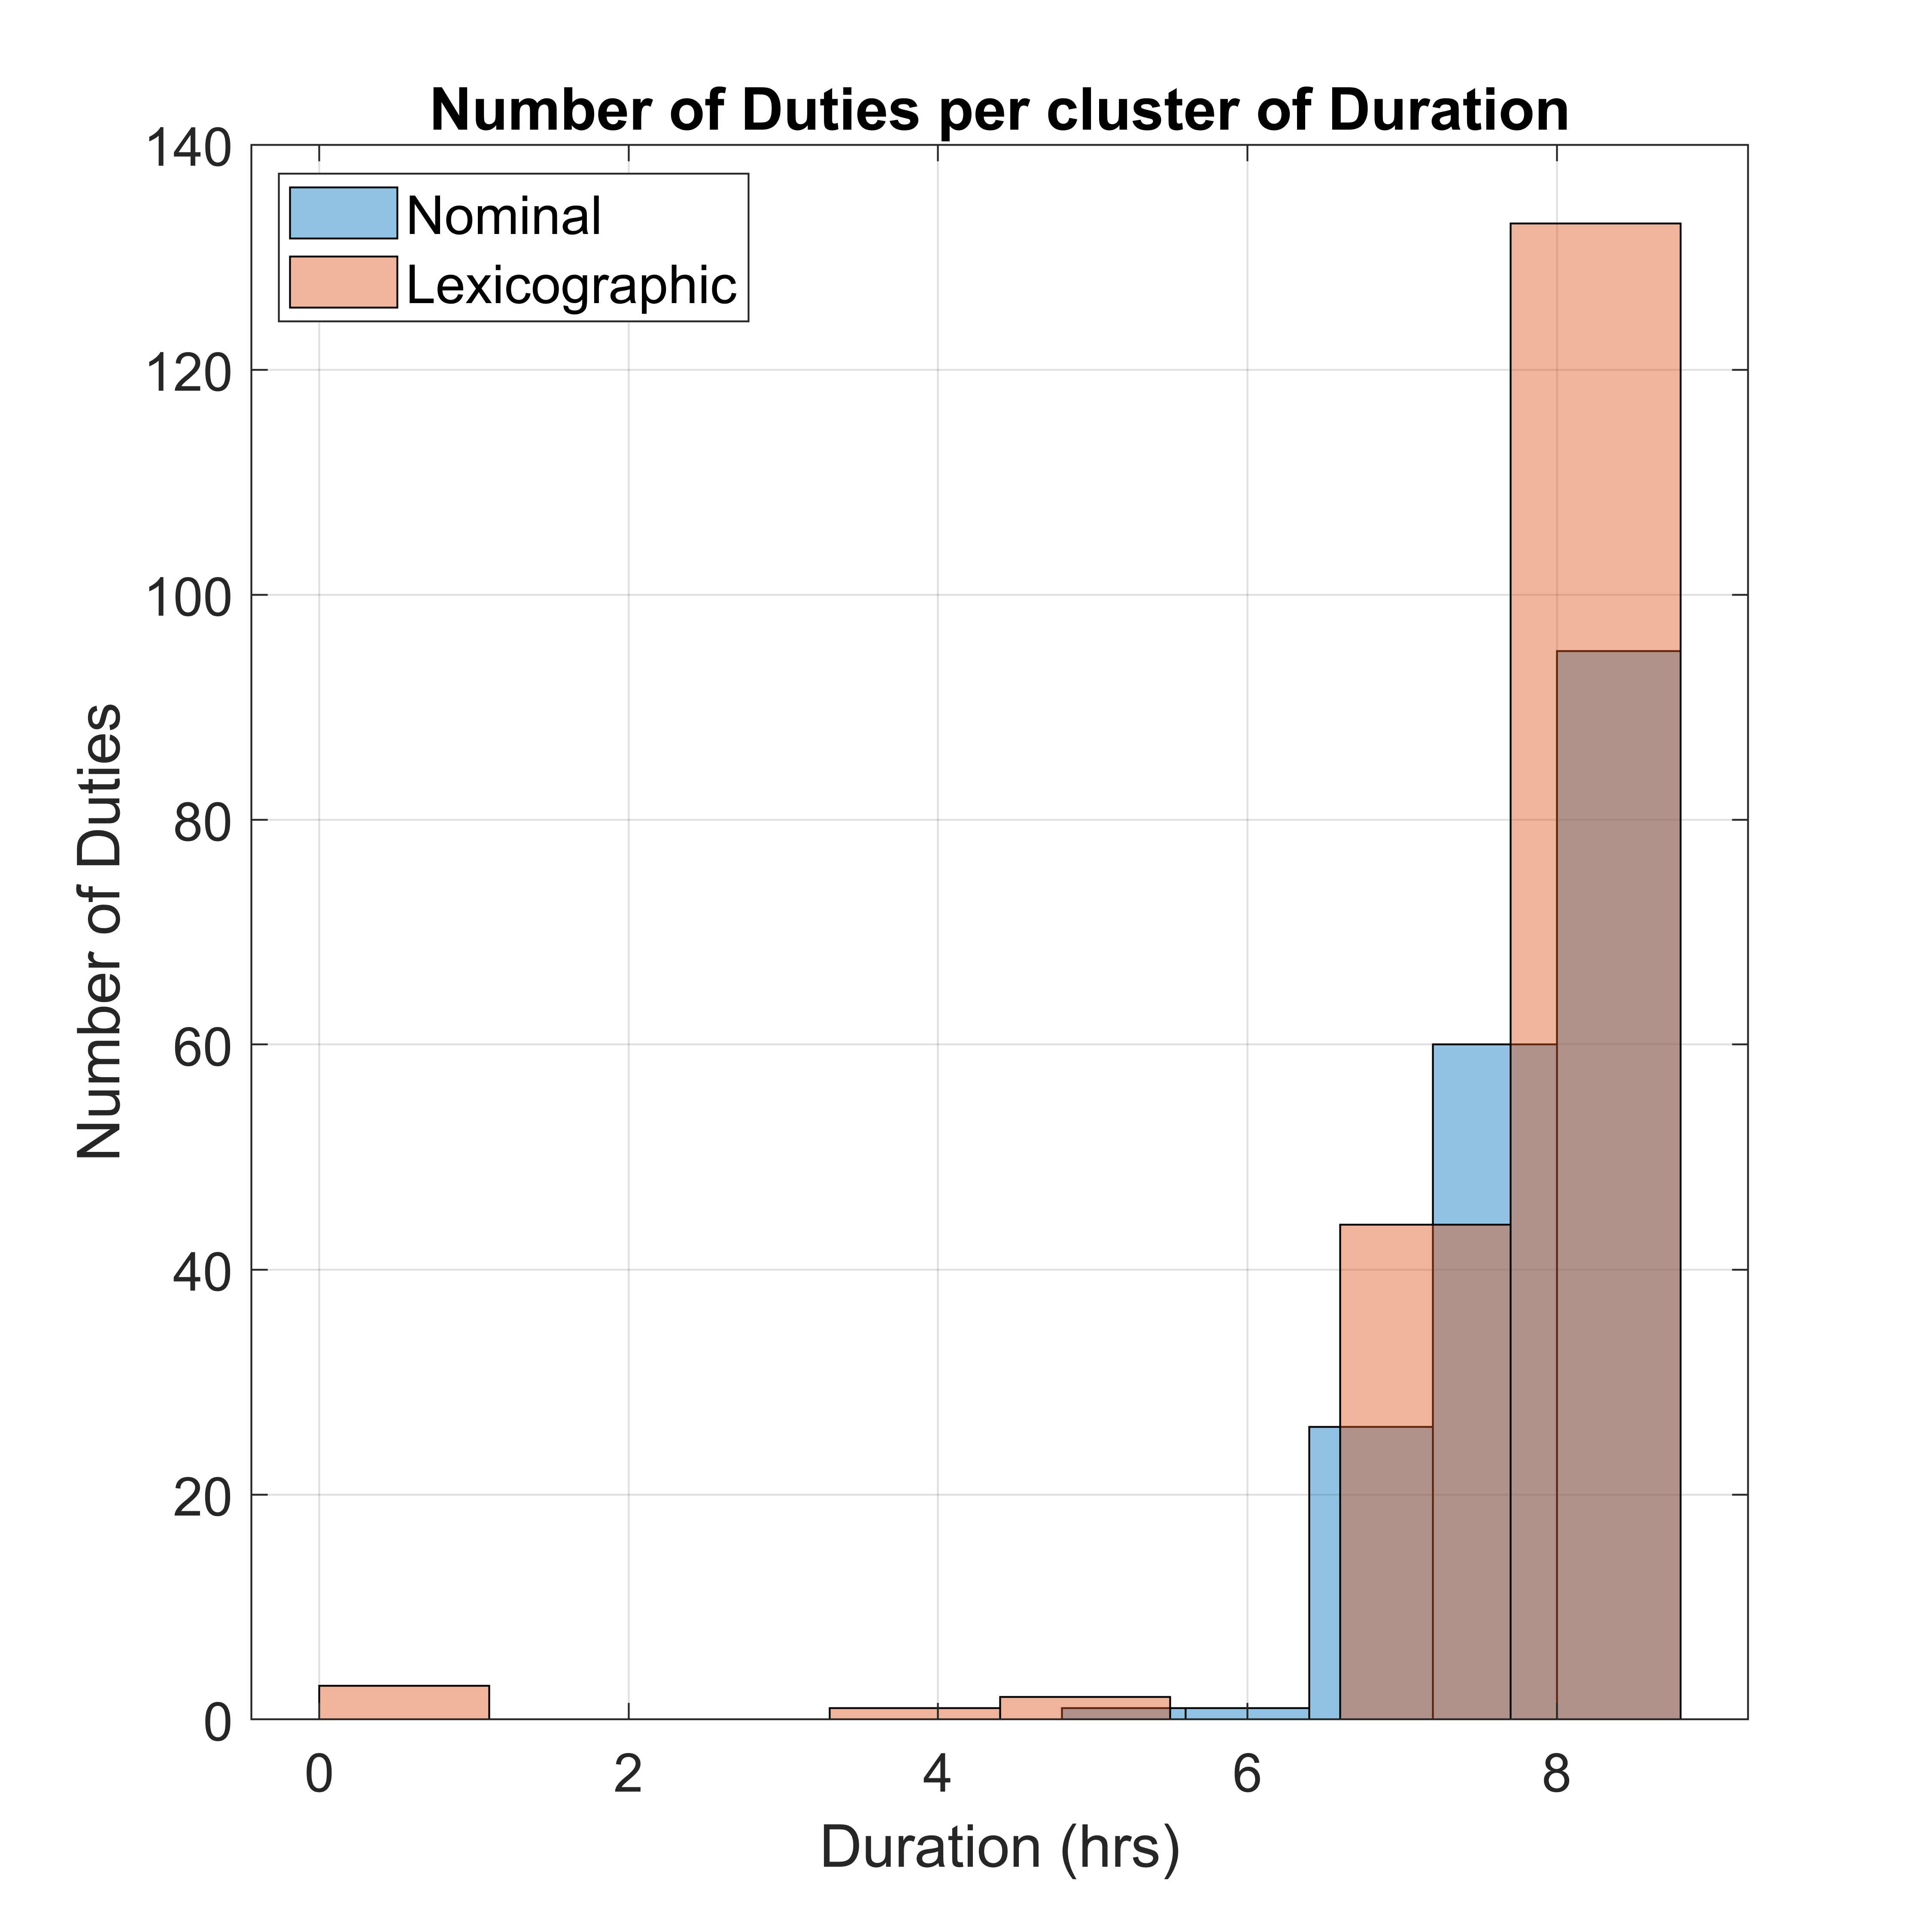
\includegraphics[width=0.46\linewidth]{[3] - chapter/nominal_vs_lexicographic.png}
    }%\end{center}}%end of picture #2
    \qquad
    %picture #2
    \centering
    \subfloat[Table comparing the characteristics of the two schedules.]{\raisebox{9em}{\begin{tabular}{|c|c|c|}
        \hline
        \textbf{Schedule} & \multicolumn{2}{|c|}{ \textbf{Characteristics}} \\
        \hline
         & \texttt{Makespan} &  \texttt{Minimum}  \\
        \hline
        Nominal & 08:25 & 05:15 \\
        \hline
        Lexicographic & 08:25 & 00:00 \\
        \hline
    \end{tabular}}}%
    \caption{Comparison of the Lexicographic and recovered-(i.e. nominal) schedules.}
    \label{fig: Nominal vs Lexicographic.}
\end{figure}

\vspace{\baselineskip}
\noindent
As we can see, the lexicographical schedule maintains the same makespan as the nominal, however is quite more tightly concentrated on duties lasting between 6-7 hours, and also has duties lasting considerably less, even down to duties of zero length.
%%%%%%%%%%%%%%%%%%%%%%% this tell us that then when we appply uncertainty

\vspace{\baselineskip}
\noindent
To determine the robustness of the lexicographic schedule to uncertainty, we apply the \texttt{reduced} and \texttt{augmented} instances for each of the $U:$ $\pm30\%$,$\pm40\%$,$\pm50\%$, and observe the effects each has on this newly generated schedule, in comparison to the previously observed effects on the nominal schedule.

%%%%%%%%%%%%%%%%%%%%%%%%%%%%%%%%%%%%%%%%%%%%%%%%%%%%%%%%%%%%%%%%%%%%%% Table %%%%%%%%%%%%%%%%%%%%%%%%%%%%%%%%%%%%%%%%%%%%%%%


\begin{table}
\small
    \centering 
    \begin{tabular}{|c|c|c|c|c|c|c|c|}
        \hline
        \rowcolor{Gainsboro!90}
        \multicolumn{2}{|c|}{\textbf{Schedule}} & \textbf{LexOpt} & \textbf{Total Time} & \multicolumn{3}{|c|}{ \textbf{Duties (HH:mm)}} & \textbf{Overrun Duties} \\
        \hline
        \multicolumn{4}{|c|}{ }  & \texttt{Makespan} & \texttt{Minimum} & \texttt{Average} &   \\
        \hline
        \multicolumn{2}{|c|}{\textbf{Instance}} &\multicolumn{6}{|c|}{ }\\
        \hline
        \multirow{4}{*}{$U$: $\pm30\%$} & \multirow{2}{*}{\texttt{reduced}} & \cmark & 1,395:54 & 10:49 & 00:00 & 07:37 & 43\\
        \cline{3-8}
         & & \xmark & 1,395:50 & 10:46 & 04:35 & 07:37 & 44\\
        \cline{2-8}
         & \multirow{2}{*}{\texttt{augmented}}& \cmark& 1,456:10 & 10:53 & 00:00 & 07:57 & 58 \\
         \cline{3-8}
         & & \xmark & 1,452:38 & 10:46 & 04:16 & 07:56 & 60\\
        \hline
        \multirow{4}{*}{$U$: $\pm40\%$} &\multirow{2}{*}{\texttt{reduced}}& \cmark& 1,427:18 & 12:16 & 03:38 & 07:47 & 64  \\
         \cline{3-8}
         & & \xmark & 1,416.47 & 11:29 & 04:00 & 07:44 & 66\\
        \cline{2-8}
         &\multirow{2}{*}{\texttt{augmented}}&\cmark & 1,444:57 & 11:45 & 00:00 & 07:53 & 68\\
         \cline{3-8}
         & & \xmark & 1,442:05 & 11:41 & 04:34 & 07:52 & 68\\
        \hline
        \multirow{4}{*}{$U$: $\pm50\%$} &\multirow{2}{*}{\texttt{reduced}}& \cmark& 1,387:40 & 12:15 & 00:00 & 07:34 & 57  \\
         \cline{3-8}
         & & \xmark & 1,386.40 & 12:15 & 03:20 & 07:34 & 58\\
        \cline{2-8}
         &\multirow{2}{*}{\texttt{augmented}}&\cmark & 1,445:08 & 12:22 & 00:00 & 07:53 & 79 \\
         \cline{3-8}
         & & \xmark & 1,445:31 & 12:19 & 03:41 & 07:53 & 79\\
        \hline
    \end{tabular}%
    \medbreak
    \caption{Table compares the Lexicographic\footnote{Represented with (\cmark)} and recovered\footnote{Represented with (\xmark)} disturbed versions of the Nominal schedule. }
    \label{table: Nominal vs Lexicographic}
\end{table}

\vspace{\baselineskip}
\noindent
As we can see from Table \ref{table: Nominal vs Lexicographic}, the Lexicographic schedule performs only marginally better than the nominal schedule in one of the two evaluation criteria. Namely, it performs marginally better in terms of the number of duties overrun since as observed on the final column of the table there are consistently less duties overrun in the lexicographic schedule compared to the nominal. However, it is marginally outperformed in terms of the makespan by the disturbed nominal schedule. 

\vspace{\baselineskip}
\noindent
Taking into consideration the above set of results, one can argue that it is questionable to call the Lexicographic schedule \textbf{more robust} than the nominal one. However, in reality it depends on the scheduler to decide which of the two criteria is of more significance for Royal Mail. Namely, is it more important for Royal Mail, for drivers to have a shorter maximum duty length \textit{L} or would they rather have less duties running longer than the pre-defined threshold. Arguably, a pragmatic approach would conclude that it is considerably more important to have a schedule that ensures that the least amount of duties possible end up crossing the \textit{L'} threshold. That is since the costs that could be incurred from overtime compensation due to a substantial amount of duties overruning are most likely going to be substantially higher compared to a handful of minutes increase in the length of the longest lasting duty (i.e. makespan). Hence, it is our opinion that the Lexicographic schedule can be characterised as more robust due to its lower allowance of duties running very long, despite its longer lasting makespans. 


\subsection*{Minimisation of the Squared Completion Time}
The secondary method that we would like to check, in our quest to enhance the robustness of our nominal schedule is that of the \textit{Minimisation of the Squared Completion Time}. This is a slightly transformed formulation that stems from the Makespan Scheduling formulation of Section \ref{section:Makespan Scheduling-content} of Chapter \ref{chapter: 2-Evaluating Royal Mail Historical Data}. The reasoning behind the choice of this method is two-fold. Firstly, a makespan scheduling based formulation loosely guarantees a well-balanced schedule. This would most likely translate to a schedule where a minimal amount of duties end up overrunning. Moreover, by slightly tweaking the objective function, and instead of minimising the makespan we refocus our formulation towards minimising its square, we will target the longer-lasting duties significantly more. That is because by minimising its square we effectively penalise significantly more the longer lasting duties. This idea stems from the philosophy followed in linear regression. The transformed formulation that we will be applying can be seen below:

%%%%%%%%%%%%%%%%%%%%%%%%%%%%%%%%%%%%%%%%%%%%%%%%%%%%%%%%%%%%%%%%%%%%%%%%%%%%%%% Maths %%%%%%%%%%%%%%%%%%%%%%%%%%%%%%%%%%%%%%%%%%%%%%%%%%%%%%%%%%%%%%%%%%%%%%%%%%%%%%

\vspace{\baselineskip}
\begin{equation}
\label{equation: Makespan Squared Scheduling}
\begin{aligned}
&\text{minimise}
%& & y_{i}  \\ %\todo{why y and and not yi}
& & y^2  \\ 
& \text{subject to}
% & & y_{i} = \sum _{j=1}^n x_{i,j}p_{j}  \;\;\; &\forall \; i \in D\tag{1}\\   
& & y \geq \sum _{j=1}^n x_{i,j}p_{j}  \;\;\; &\forall \; i \in D\\   
& & &\sum _{i=1}^m x_{i,j} = 1 \;\;\; &\forall \; j \in B\\
% & & &\sum _{j=1}^n x_{i,j}p_{j} \leq f_{i}-s_{i} \;\;\; &\forall \; i \in D\\ %{\color{red} we deleted the constraint that involves the length of duty being less than end-start.}
& & & y\geq 0  \\
& & & x_{i,j} \in  \{ 0,1 \} \;\;\; &\forall \; j \in B, \; i \in D\\
\end{aligned}
\end{equation}

\vspace{\baselineskip}
\noindent
The formulation is identical to equation \ref{equation: Makespan Scheduling} of Chapter \ref{chapter: 2-Evaluating Royal Mail Historical Data}, except for the objective function. The objective is to get the \textbf{minimal} possible squared of \textbf{makespan} as opposed to previously simply minimising the makespan.
%%%%%%%%%%%%%%%%%%%%%%%%%%%%%%%%%%%%%%%%%%%%%%%%%%%%%%% Double Figure %%%%%%%%%%%%%%%%%%%%%%%%%%%%%%%%%%%%%%%%%%%%%%%%%%%%%%%%%%%%%%%%%%%%%%%%%%%

\begin{figure}%
    \centering
    \subfloat[Histogram showing the comparison of distributions of block per duty length of the two schedules.]{%\begin{center}
    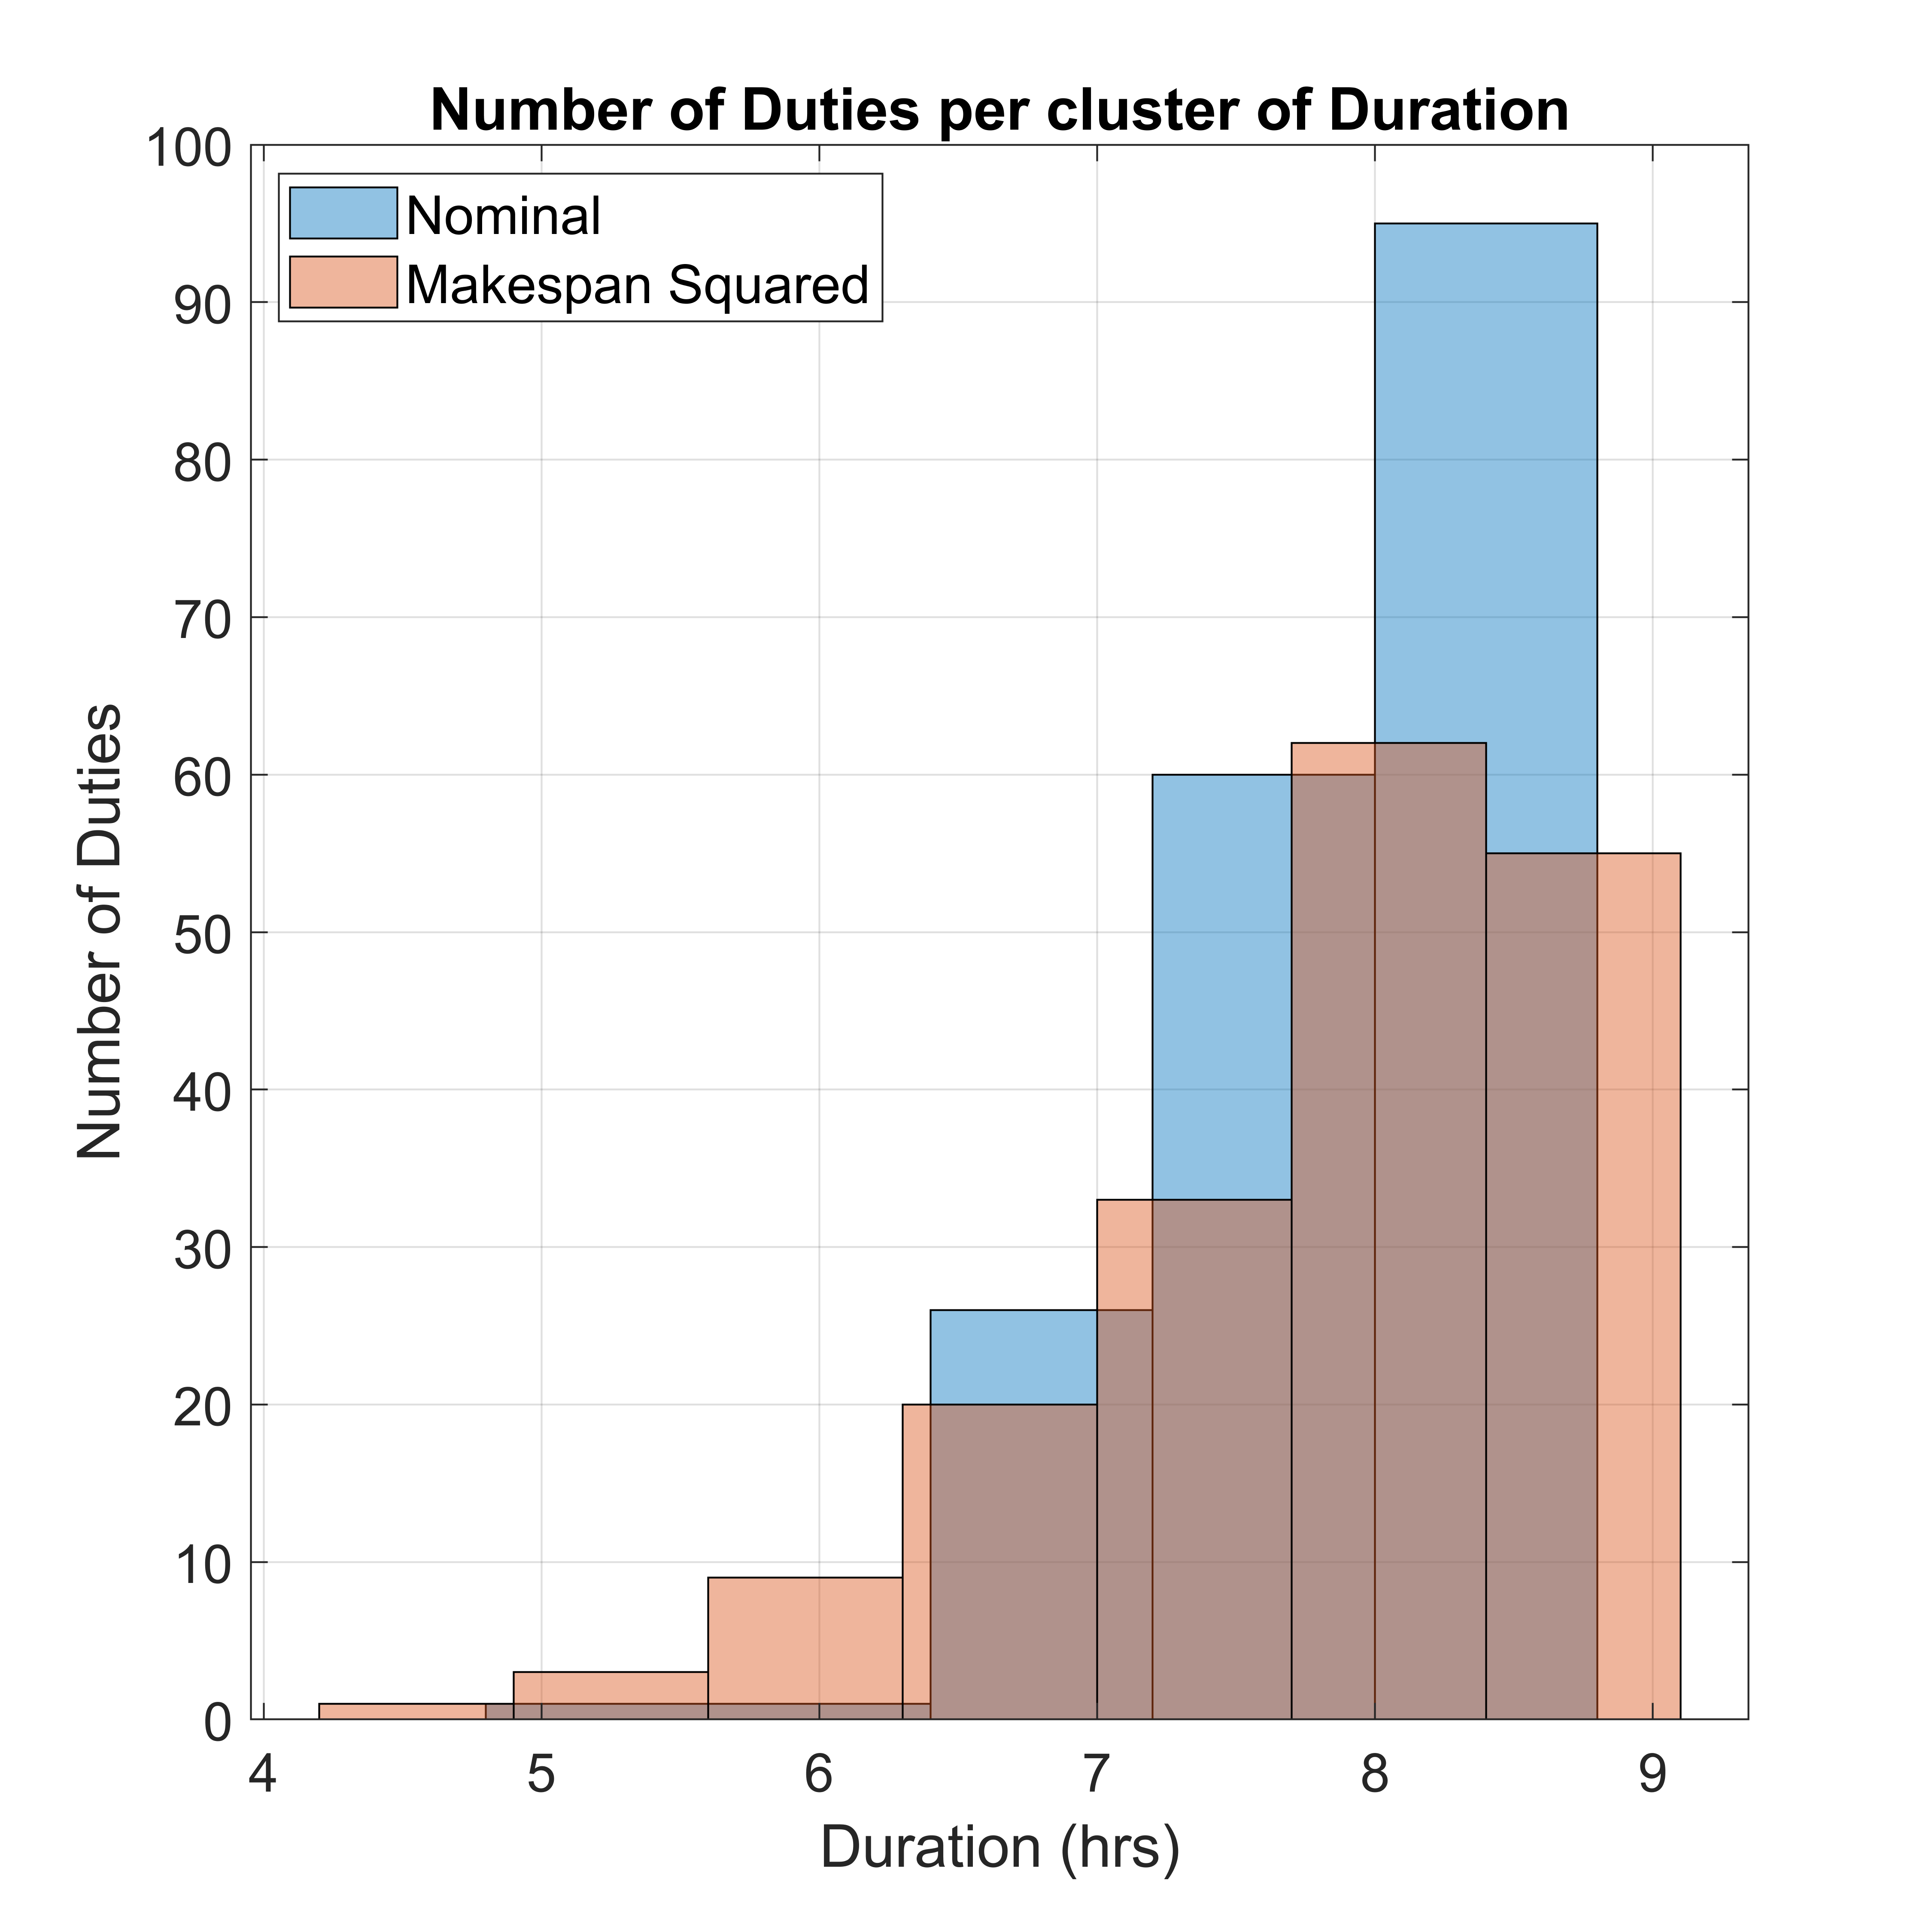
\includegraphics[width=0.46\linewidth]{[3] - chapter/nominal_vs_squared.png}
    }%\end{center}}%end of picture #2
    \qquad
    %picture #2
    \centering
    \subfloat[Table comparing the characteristics of the two schedules.]{\raisebox{9em}{\begin{tabular}{|c|c|c|}
        \hline
        \textbf{Schedule} & \multicolumn{2}{|c|}{ \textbf{Characteristics}} \\
        \hline
         & \texttt{Makespan} &  \texttt{Minimum}  \\
        \hline
        Nominal & 08:25 & 05:15 \\
        \hline
        Makespan Squared & 09:04 & 04:34 \\
        \hline
    \end{tabular}}}%
    \caption{Comparison of the Makespan Squared and Makespan Optimised (nominal) schedules.}
    \label{fig: Nominal vs Squared.}
\end{figure}


\vspace{\baselineskip}
\noindent
As one can determine from Figure \ref{fig: Nominal vs Squared.} the two schedules as expected resemble each other quite a lot, given that they stem from a principally similar formulation. However, we can notice that Makespan Squared model has a slightly longer bandwidth that also contributes to each longer lasting makespan. We subsequently, apply the disturbed instances on it to see its robustness against those uncertainty components, compared to the nominal schedule.

\vspace{\baselineskip}
\noindent
Through a thorough analysis of Table \ref{table: Nominal vs Makespan Squared}, one can determine that the Makespan Squared formulation performs substantially sub-par when compared to the nominal Schedule in both criterion. The makespan is consistently higher, and there are generally more duties that end up overrunning compared to the nominal schedule.

\vspace{\baselineskip}
\noindent
As a result, overall we can conclude that the lexicographically generated schedule is the most robust schedule. That is determined by the results of our experiments and the comparison of the results that show that the recovered version of the LexOpt schedule that makes the least amount of compromise with respect to the minimisation of its Makespan, while achieving the robustness quality since it consistently has the least number of overrun duties.
%%%%%%%%%%%%%%%%%%%%%%%%%%%%%%%%%%%%%%%%%%%%%%%%%%%%%%%%%%%%%%%%%%%%%% Table %%%%%%%%%%%%%%%%%%%%%%%%%%%%%%%%%%%%%%%%%%%%%%%


\begin{table}
\small
    \centering 
    \begin{tabular}{|c|c|c|c|c|c|c|c|}
        \hline
        \rowcolor{Gainsboro!90}
        \multicolumn{2}{|c|}{\textbf{Schedule}} & \textbf{Squared} & \textbf{Total Time} & \multicolumn{3}{|c|}{ \textbf{Duties (HH:mm)}} & \textbf{Overrun Duties} \\
        \hline
        \multicolumn{4}{|c|}{ }  & \texttt{Makespan} & \texttt{Minimum} & \texttt{Average} &   \\
        \hline
        \multicolumn{2}{|c|}{\textbf{Instance}} &\multicolumn{6}{|c|}{ }\\
        \hline
        \multirow{4}{*}{$U$: $\pm30\%$} & \multirow{2}{*}{\texttt{reduced}} & \cmark & 1,405:43 & 11:19 & 03:57 & 07:40 & 83\\
        \cline{3-8}
         & & \xmark & 1,395:50 & 10:46 & 04:35 & 07:37 & 44\\
        \cline{2-8}
         & \multirow{2}{*}{\texttt{augmented}}& \cmark& 1,457:31 & 11:36 & 04:49 & 07:57 & 73 \\
         \cline{3-8}
         & & \xmark & 1,452:38 & 10:46 & 04:16 & 07:56 & 60\\
        \hline
        \multirow{4}{*}{$U$: $\pm40\%$} &\multirow{2}{*}{\texttt{reduced}}& \cmark& 1,427:18 & 12:16 & 03:38 & 07:47 & 101  \\
         \cline{3-8}
         & & \xmark & 1,416.47 & 11:29 & 04:00 & 07:44 & 66\\
        \cline{2-8}
         &\multirow{2}{*}{\texttt{augmented}}&\cmark & 1,456:17 & 12:41 & 03:31 & 07:57 & 97\\
         \cline{3-8}
         & & \xmark & 1,442:05 & 11:41 & 04:34 & 07:52 & 68\\
        \hline
        \multirow{4}{*}{$U$: $\pm50\%$} &\multirow{2}{*}{\texttt{reduced}}& \cmark& 1,392:27 & 12:54 & 03:23 & 07:36 & 99  \\
         \cline{3-8}
         & & \xmark & 1,386.40 & 12:15 & 03:20 & 07:34 & 58\\
        \cline{2-8}
         &\multirow{2}{*}{\texttt{augmented}}&\cmark & 1,446:46 & 13:05 & 03:37 & 07:54 & 88 \\
         \cline{3-8}
         & & \xmark & 1,445:31 & 12:19 & 03:41 & 07:53 & 79\\
        \hline
    \end{tabular}%
    \medbreak
    \caption{Table compares the Makespan Squared\footnote{Represented with (\cmark)} and recovered\footnote{Represented with (\xmark)} disturbed versions of the Nominal schedule. }
    \label{table: Nominal vs Makespan Squared}
\end{table}
\vspace*{3in}
\vspace{\baselineskip}
%\chapter{Project Plan}


\section{Milestone $\#$ 1 – Formulation of model and Solving it}
\vspace{\baselineskip}
\subsubsection*{Goal}
\addcontentsline{toc}{subsubsection}{Goal}

Formulate and implement a \textit{mixed-integer linear programming} model with the aim of computing exact solutions for the dataset supplied by Royal Mail. For this milestone, the schedules generated  have complete freedom to schedule the meal-relief breaks anywhere within the atomic time blocks (representing the HGV's routes). At the same time, legality needs to be maintained by respecting the EU rules for the Driving and Working time directives. 



\vspace{\baselineskip}
\subsubsection*{Progress}
\addcontentsline{toc}{subsubsection}{Progress}

Initial model formulations have been made and currently working towards testing with synthetic data. Testing of the current model formulation with inputs from the real dataset with the goal of discovering proposed improvements to the model, is the immediate next step. This will  determine whether an exact solution is possible.



\vspace{\baselineskip}
\subsubsection*{Fallback position}
\addcontentsline{toc}{subsubsection}{Fallback position}

Given that this milestone will in principle comprise the bulk of the project a fallback position, in the event that an exact solution is not possible, is to explore the use of approximation algorithms such as the \textit{randomised rounding }approach to reach approximate solutions for the problem.



\vspace{\baselineskip}
\subsubsection*{Timetable }
\addcontentsline{toc}{subsubsection}{Timetable }

Conducting critical analyses of the improvements to the model that arise from testing is to be undertaken until mid-February with the goal of determining by then whether an exact solution is possible. Depending on that outcome, by the end of February the focus will shift either to getting an approximate solution through approximation algorithm techniques or focusing on pursuing Milestones $\#$ 2, $\#$ 3.



\vspace{\baselineskip}
\section{Milestone $\#$ 2 – Incorporate Company Policy Requirements}
\vspace{\baselineskip}
\subsubsection*{Goal}
\addcontentsline{toc}{subsubsection}{Goal}

Incorporate in the model the Royal Mail company policy that breaks should occur only after a certain subset of activities out of the set of possible activities undertaken by the drivers. This is to be modelled with \textit{precedence constraints}. Given the complexity that this task would introduce, approximation algorithms will almost certainly need to be explored.



\vspace{\baselineskip}
\subsubsection*{Timetable}
\addcontentsline{toc}{subsubsection}{Timetable}

Provided that Milestone $\#$ 1 has been achieved by the end of February, the period throughout March – April will be spent on this second milestone. If Milestone $\#$ 1 has not been achieved and implementation of the fallback position is necessary, an extra month will approximately need to be spent on Milestone $\#$ 1.



\vspace{\baselineskip}
\section{Milestone $\#$ 3 – Additional Constraints}
\vspace{\baselineskip}
\subsubsection*{Goal}
\addcontentsline{toc}{subsubsection}{Goal}

Incorporate jobs that have a time-window limitation assigned to them, modelled by fixed atomic blocks.



\vspace{\baselineskip}
\subsubsection*{Timetable}
\addcontentsline{toc}{subsubsection}{Timetable}

Whether or not this milestone can be pursued will depend on the other two milestones.



\vspace{\baselineskip}
\subsection*{Final Report Preparation}

\subsubsection*{Timetable}
\addcontentsline{toc}{subsubsection}{Timetable}

Expected to commence after the $``$Project health check-up$"$  meeting during the week 11/05 - 15/05 and is expected to last for one-month, hence from the 17/05 until \textbf{17/06} which is the \textbf{report submission deadline}.





\chapter{Evaluation}
\label{chapter: Evaluation}

This chapter contains a discussion that aims to evaluate the contributions of this report and provide a critical appraisal of the experiments and techniques used.

\vspace{\baselineskip}
\noindent
This dissertation is a continuation of the Red October project which refers to the partnership of the Royal Mail Data Science Group with Imperial's Computational Optimisation Group. The project as the title suggest mostly deals with data analysis processes and concludes with an examination of uncertainty. The original direction of the project focused more on the study of uncertainty. However, after a meeting with our Industrial Liaison at the start of the year both parties realised that a thorough examination of the dataset was going to be a substantially bigger task than originally through. That is because this body of work is the first attempt at analysing the dataset described in Chapter \ref{chapter: Problem Definition}. This project's purpose was hence slightly amended, and its new objective became to serve as a stepping stone for future methodological explanations based on the findings of our analysis of the dataset. The high-level objectives of the project resembled part of those of a previous PhD thesis \cite{natashapage}, which also included the first exploration of a different dataset provided by Royal Mail.

\vspace{\baselineskip}
\noindent
Those high-level objectives of extracting the maximum amount of insights possible from this dataset were explored in Chapters \ref{chapter: Problem Definition},\ref{chapter: 2-Evaluating Royal Mail Historical Data}. We evaluated the schedules that are currently run by Royal Mail and used them as the basis to develop more efficient schedules. The thought process behind this task was to generate a finding for our industrial liaison that illustrates the room for optimisation that exists. Although our findings are not concrete proof that our schedules would work for Royal Mail since they are based on theoretical assumptions they provide an insight into what is possible in regards to efficiency. Having obtained a lower bound that shows what schedules we are capable of developing, we can then use this insight to gradually create evermore practically realisable schedules by shifting our assumptions towards more life-resembling postulates. 

\vspace{\baselineskip}
\noindent
The uncertainty portion of the dissertation attempts to cover new ground with respect to findings that compare the performance of various methodologies. More specifically in Chapter \ref{chapter:Benchmark Instances} we compare a total of three methodologies with respect to the efficiency and robustness to uncertainty of the schedules they generate. Those are the non-pre-emptive Makespan Scheduling formulation of Section \ref{section:Makespan Scheduling-content} as well as schedules from the Lexicographic Optimisation methodology and the Squared Completion time method.  

\vspace{\baselineskip}
\noindent
The uncertainty components are based on \textit{box} uncertainty sets of various sizes. Our initial goal was to also explore the effects of the ellipsoidal uncertainty sets\footnote{Mentioned in Section \ref{section:background uncertainty} of Chapter \ref{chapter: Background}} however, the study of uncertainty was added as an additional topic towards the end of the project timeline. As a result, although an initial attempt to incorporate ellipsoidal uncertainty sets was made we decided to abandon further pursuing it and instead propose it as one of the future direction that we deemed worthwhile investigating in Chapter \ref{chapter: Future Directions}. However, when providing an appraisal of Chapter \ref{chapter:Benchmark Instances} we are obliged to mention that this results in a potentially non-complete study of the disturbance effects. It is critical for the uncertainty study to provide meaningful insights to also explore the effects that the ellipsoidal uncertainty sets will have on our schedules, since they could be use approximate the effects of more complex uncertainty sets as discussed in \cite{vertsimas}.

\subsection*{Classification of Redundant Activities}
As mentioned in Section \ref{section: Redefined Dataset} of Chapter \ref{chapter: Problem Definition} we created a series of additional instances that we labelled \textbf{Redefined Historical Schedules}. The generation of those instances was performed by deleting a series of redundant activities from the dataset. More specifically, we classified a collection of duties as \textit{non-useful} and proceeded to erase them from within their blocks. The classification of the activities as \textit{useful} or not was not performed in consultation with our Industrial Liaison. Instead we used as a criterion the frequency of occurrence of each activity to determine its level of importance. Using our self-determined classification we conducted the experiments involving the Redefined instances and presented them to our industrial partners in an interim presentation. 

\vspace{\baselineskip}
\noindent
During the preparation of the presentation, it was noticed that the classification of the activities might be ill-advised. This observation stems from Table \ref{table: Useful vs Non-Useful Activities} in Section \ref{section: Redefined Dataset}. As we can see we mistakenly classified the activities \texttt{Park Vehicle}, \texttt{Check}, \texttt{Clean} as \textit{non-useful}. However, we later determined that all three of those activities require the presence and control of the HGV driver. As a result, they cannot be characterised as \textit{non-useful}. It is only the \texttt{Distribution/Processing} activity that can be regarded as \textit{non-useful}.

\vspace{\baselineskip}
\noindent
Although this observation was uncovered in too late a stage, further research showed that the effect on our results is minimal. 

\subsection*{Optimality Gap in Redefined Optimised Schedules}
In Section \ref{section:Makespan Scheduling-content} of Chapter \ref{chapter: 2-Evaluating Royal Mail Historical Data}, we conclude our analysis of the Makespan Scheduling formulation by applying formulation (\ref{equation: Makespan Scheduling}) on the Redefined instances. In observing the results from that experiment we observed that the generated schedules had not achieved their full potential with respect to the minimisation of their makespan. More specifically we observed that the makespan achieved was greater than the longest lasting block observed in the instance that it was based on.

\vspace{\baselineskip}
\noindent
The reasoning behind this under-performance was founded in the fact that during the generation of the schedule the timer upper of $10^3 \; seconds$ was triggered. Hence, naturally we did not obtain the optimal solution for the case and as a result an optimality gap existed between the true optimal schedule and our result. We decided not to amend that optimality gap by changing the timer trigger because that would render the comparison of all our results inconsistent. However, we could claim that for the purposes of assisting Royal Mail's efforts it might have been advisable to close that optimality gap and obtain the true optimum solution.

\subsection*{Impracticable Pre-emptive Schedules}
In Section \ref{section: Pre-emptive} of Chapter \ref{chapter: 2-Evaluating Royal Mail Historical Data} we transform our previously utilised formulation of Makespan Scheduling into an equivalent pre-emptive formulation. The purpose of this transformation of our model is to use the transformed model to obtain a an approximation of the \textbf{theoretical optimal schedule}. 

\vspace{\baselineskip}
\noindent
We were indeed able to reduce the optimality gap to the theoretical limit by applying this pre-emptive formulation. As mentioned in Chapter Chapter \ref{chapter: 2-Evaluating Royal Mail Historical Data} however, this formulation violated one of the assumptions outline in Section \ref{section: 4.1}. The practical implications of generating a schedule that violates this postulate are quite significant. The structure of such a schedule render it impossible to implement from the perspective of Royal Mail. A pre-emptive schedule is not realistic in terms of its implementation because it would require the HGV drivers to carry out activities in a chaotic sequence. 

\vspace{\baselineskip}
\noindent
More specifically, the blocks of an instance that we schedule with each formulation have certain semantics attached to them. As outlined in Section \ref{section: 4.1} we can afford to neglect them as long as the non-pre-emptive nature of our final schedule is preserved. In more detail, the blocks contain certain activities within the spectrum of a round-trip. Within a block those activities are ordered according to a logical sequence. For instance, as we had discussed in Section \ref{section: Data Exploration} of Chapter \ref{chapter: Problem Definition}, we expect an \texttt{unload} activity to occur in direct succession to a \texttt{travel} activity. By maintaining a non-preemptive formulation and through obeying assumption (1) of Section \ref{section: 4.1} that logical sequence is preserved. As a result, the practical utility of such a schedule is also preserved. Such a schedule has true value for Royal Mail since it can be implemented on the floor of a MC with little effort, as it is fundamentally based on a re-arrangement of the Historical schedule.

\vspace{\baselineskip}
\noindent
In contrast, the schedules generated from a pre-emptive formulation that consequently violate assumption (1), although more efficient with respect to the objective, have no practical utility for Royal Mail. That observation is based on two pitfalls of the pre-emptive schedule.

\vspace{\baselineskip}
\noindent
Firstly, it would take a tremendous effort of a re-definition of Royal Mail's company policies for such schedules to be allowed. That is because implementing those schedules in practice would require a fundamental re-organisation of the routes followed by drivers. That is since the pre-emptive schedules pay no regard to the reasoning behind the crafting of routes but are only concerned with most efficiently fitting activities into duties. Moreover, since we neglect information regarding distance between the various external locations\footnote{As mentioned in Section \ref{section: Data Cleaning} of Chapter \ref{chapter: Problem Definition}} we could have successive travel legs schedule that are at the complete opposite ends of the area for which the MC is responsible for.

\vspace{\baselineskip}
\noindent
Secondly, the pre-emptive schedules could never be realised in their true form because they tend to schedule futile sequences of activities. More specifically since we allow the pre-emptive schedules to breakdown the pre-defined structure of blocks when observing the sequence of activities schedule by the solver we notice the occurrence of sequence of activities that are impossible. For instance, we observed the successive scheduling of \texttt{unload} activities one after the other. As one can easily determine that sequence of activities is completely futile as the second \texttt{unload} activity will be scheduled completely in vain. Once again, this phenomenon is observed because we allow our formulation to disobey assumption (1) and hence the semantics associated with each block.

\vspace{\baselineskip}
\noindent
All in all, the approximation for the theoretical limit for the makespan that we obtained from the pre-emptive formulation can only be characterised as a practically obtainable lower bound. It can only be characterised as practical because it can actually be obtained from the output end of a solver but not because it can be practically implemented by our Industrial Liaison. 




%\chapter{Conclusion}
TBC
\chapter{Concluding Remarks}
\label{chapter: Future Directions}

%conclusion lambanontas upopsi oti o reader kserei ti exei ginei sto thesis
The goal of this final chapter is to conclude this report by reiterating the main contributions of this dissertation, and state a collection of promising ideas for future exploration that stem from the work enclosed in this report.

\section{Conclusion}


In this dissertation, we provide an initial exploration of the opportunity for optimisation of schedules based on the dataset supplied by Royal Mail, as well as an initial step towards the development of an efficient but also robust schedule against uncertainty. Our focus with respect to locating the room for improvement that exists in the historical schedule has been focused on the solution of various \textit{Mixed-Integer Optimisation Problems}, motivated in part by the fact that such formulations enable us to optimised various aspects of the historical schedules. Our goal in optimising those aspects of the historical schedules is to provide solutions for improvements inside a sphere of different factors ranging from employee quality of life, to cost-savings for the company.


\vspace{\baselineskip}
\noindent
In Section \ref{section:Makespan Scheduling-content} of Chapter \ref{chapter: 2-Evaluating Royal Mail Historical Data}, the solution of the Makespan Scheduling formulation provides us with a schedule that featured a minimised makespan. This translates to a more balanced schedule that will prevent employees working overtimes hence improving their general quality of life at work. The following model involved a formulation that attempted to minimise the number of duties required to execute the workload at hand. As seen in Sections \ref{section:minimise duties}-\ref{section: maximise blocks} the solutions provided, outlined a series of schedules that improved on the current schedule both on the employee quality of life and company cost-savings fronts. Namely, the schedules generated by formulation (\ref{equation: Minimise Duties}) minimised the number of duties required. Consequently, the majority of employees could afford to work marginally less, since there were less duties to be completed, and concurrently, Royal Mail could have cost-savings from the reduction in duties since it might possible to place some willing employees to a part-time work schedule. Similarly, formulation (\ref{equation: M3}) maximised the number of blocks that can be processed as we decrease the maximum duty length of the schedule. Our findings indicated that we can generally afford a reduction in the maximum duty length without impacting our processing capacity significantly. Hence, provided Royal Mail is able to implement such schedules with a reduction in the maximum duty length we will have generated an improvement in the quality of life of employees as well as possibility for cost-saving by placing employees on part-time duties.

\vspace{\baselineskip}
\noindent
Finally in Chapter \ref{chapter:Benchmark Instances} we make the first steps towards the formulation of a schedule that is concurrently efficient with respect to the makespan criterion but also remains robust against uncertainty. We start by applying uncertainty components of various sizes to the schedule generated through formulation (\ref{equation: Makespan Scheduling}) of Section \ref{section:Makespan Scheduling-content}. We then optimise those schedules with the Makespan Scheduling formulation. We then compare the optimised disturbed schedules with the recovered version of the nominal. We repeat the same process for schedules generated from two new formulations, the lexicographic and completion time squared models. In the end, we compare all three schedules and determine that the schedule that stems from the lexicographic optimisation is the most robust, and makes the smallest compromise in its makespan efficiency. 

\section{Future Directions}
We conclude this final chapter by enclosing directions for future exploration that were deemed to be worthwhile for further research, upon conversation with our \textit{industrial liaison}, Royal Mail. These ideas are largely an extrapolation of the work presented in this dissertation in the direction of a more practical application of the ideas developed in this report. The fulfilling of the directions outlined below would render our solutions more realistically applicable from the perspective of Royal Mail, since they involve the addition of practical constraints faced by Royal Mail. In contrast the work of this dissertation is largely theoretical and is hopes to discover the theoretical boundaries for optimisation that exist in the context of the problem that we have studied. 

\subsection*{Scheduling Meal-Reliefs}
\label{section: Addition of the Meal Relief Constraint}
The first direction for future investigation concerns the provision of schedules that comply with the Meal-Relief constraint enforced by EU regulations around \textbf{driving} and \textbf{working time directives}, as seen in Appendix \ref{section: EU rules}. Meal-Reliefs are one of the activities observed in the data, as seen in Chapter \ref{chapter: Problem Definition}. However, for the purposes of the Meal-Relief constraint, they are considered a special kind of activity since their location inside a schedule dictates whether the overall schedule is compliant with the EU regulations. Consequently, the decision regarding the time that these activities are scheduled involves the addition of a new type of scheduling constraint. 

\vspace{\baselineskip}
\noindent
In practice, this involves the addition of two new scheduling constraints to our models, one for the driving time and one for the working time directives. These two constraints will render certain schedules infeasible if they do not satisfy both directives. 

\vspace{\baselineskip}
\noindent
Even though it is extremely interesting to explore from an algorithmic point of view, after consulting with our industrial liaison, we determined that it was out of scope for the purposes of this dissertation. Our goal through this project is to provide schedules that explore the boundaries of what is possible in the context of this problem. In contrast, choosing to implement the Meal-Relief constraint would allow us to search for efficient schedules from within a rather narrow subset of the overall feasible set, hence preventing us from approaching the boundaries of global optimally. Moreover, as we were informed by the Royal Mail Scheduling staff, enforcing the Meal-Relief constraint, is largely an \textit{ad-hoc} operation that they tend to perform at the last stage of the schedules' design, which also takes into account the various peculiarities related to each MC's fleet of drivers. For instance, drivers at each MC may be accustomed to taking their Meal-Relief breaks only at specific locations and at specific times within their duty. Hence, enforcing a high-level version of the Meal-Relief constraint that does not take into account those minor but important details would not prove effective in reality. As a result, focusing on further exploring this aspect of the problem without considering such human factors that are not captured by the dataset, and can only be examined within Royal Mail's infrastructure was determined to be not worthwhile pursuing at this stage of the project. 

\vspace{\baselineskip}
\noindent
Provided, that we can gain access to this information and consult with each MC's stakeholders to take into account their requests, and implement them in the form of various optimisation constraints, the enforcement of the Meal-Relief constraint can be reduced down to a mere addition of a constraint to our model. The \textbf{working time directive} is to be respected by making sure that the \textbf{duration} of a \textit{duty} is compliant with the regulation. On the contrary the \textbf{driving time directive} is examined at the \textbf{block} level, and has to be respected between adjacent blocks.  The collection of travel legs featured within each block are those that determine the feasibility component, regarding the \textbf{driving time} regulation. 

\subsubsection*{Driving Time Directive}

\vspace{\baselineskip}
\noindent
Ideally, it should take place at the end of a shift, at which point the \textit{driving time} limit has been exhausted. However, in the case that prior blocks have consumed a large part of the 4.5 hour driving buffer such that the following block would violate the regulation, the meal relief has to be brought forward, and scheduled between the blocks.   

\subsubsection*{Working Time Directive}

 Technically, \texttt{Meal-Relief} activities, are at the moment actually scheduled inside the blocks featured in our proposed schedules since as explained in the Data Cleaning section (\ref{section: Data Cleaning}) the \texttt{Meal Relief} activity was one of the \textbf{useful} activities that we preserved insider our blocks during the Data Cleaning procedures we followed. Hence, as far the implementation of the Meal Relief Constraint is concerned, rendering our \textit{proposed schedules} legal with respect to this constraint is simply a matter of moving the \texttt{Meal Relief} activities in the right place within the space of a duty. 
 
 \vspace{\baselineskip}
\noindent
 Moreover, we anticipate that the addition of these constrains to our models, will make the process of finding an optimal solution less complicated, as opposed to without them since we will be essentially \textit{tightening our feasible space}, hence it will relatively more straightforward to obtain an optimal solution. 

\vspace{\baselineskip}
\noindent
Upon conversation with our industrial liaison (Royal Mail), we decided to forego the desire to explore the \textbf{Meal Relief} constraint, as it was deemed merely a practical contribution that would not particularly expand the theoretical frontier for what is possible. 

\subsection*{Vehicle Routing Considerations}
As was discussed in the introductory chapters we do not particularly focus on the \textit{Vehicle Routing} component of the problem. By additionally implementing the \textit{routing} component, we wish to extend the aspects of the problem captured in our model, a critical sub-problem in the majority of distribution network problems.

\vspace{\baselineskip}
\noindent
We briefly investigated a glimpse of the routing aspect of the problem in section \ref{section: Pre-emptive}, where the implementation of the pre-emptive philosophy did in fact result into a \textit{re-routing} of the routes followed by drivers. However, numerous experiments that are specifically focused on the solution of the \textit{routing} problem are required to acquire an accurate and insightful understanding of the problem through this point of view.

\vspace{\baselineskip}
\noindent
 As explained, in the Data Cleaning section (\ref{section: Data Cleaning}), we eliminated certain attributes from each data entry of the dataset that were not helpful when looking at the problem from the \textit{scheduling perspective.} As seen in Appendix \ref{subsection: Eliminated Attributes} one out of those eliminated attributes, consisted of information regarding the distance between locations visited by the HGVs. In solving this problem, one could use this information and form the problem through the concept of a \textbf{graph}. \textit{Edges}, of this graph would represent the \textit{time} and \textit{distance} between locations and \textbf{nodes} would represent the various external locations themselves. Plotting these graphs, one could then rearrange the \textbf{routing} aspect of the problem to make efficiency gains.
 
\subsection*{Incorporating Deadline Constraints}
During the initial data cleaning stages of the project we observed the existence of certain blocks that contained trips that were bound with a deadline with respect to the time of their completion. Namely, such trips involve the delivery of time-sensitive packages. As explained in Section \ref{section: Data Cleaning} of Chapter \ref{chapter: Problem Definition} this packages often refer to trips to the airport, which are by nature time-constrained.

\vspace{\baselineskip}
\noindent
However, as explained in Section \ref{section: Data Cleaning} we decided to ignore such data that is related to \textbf{time-constrained packages} and determine it us out of scope for the purposes of our project. The rationale behind this decision is founded in the fact that to satisfy our objective of finding the available room for optimisation we demand total freedom as far as our ability to move the blocks from duty to duty.

\vspace{\baselineskip}
\noindent
Nevertheless, the exploration of such time-constrained trips would be of significant interest both for researchers but also for Royal Mail. For researchers such a task poses great methodological potential. Namely, these time-sensitive round-trips would place certain blocks rigidly inside the spectrum of a duty such that the solver cannot relocate them. In practice, it would be implemented as an additional optimisation constraint. As our result, this would further shrink the feasible set allowing the scheduler less room for the exploration of the optimisation bounds. From the perspective of Royal Mail, the incorporation such constraints would be highly valuable since it would make our proposed schedules more realistic. Moreover, those schedules would be easier to implement since Royal Mail's operators would not have to heuristically add those constraints and re-order the duties' sequences so that those blocks are placed rigidly in the right place. 

\subsection*{Incorporating Ellipsoid Uncertainty Sets}
As mentioned in the evaluation chapter (\ref{chapter: Evaluation}) due to the fact the study of uncertainty was a late addition to the topics explored we decided not to proceed with the addition of ellipsoid uncertainty set-based components. However, we believe that the study of the effects the application of an ellipsoid-based uncertainty components is a direction for future research that should definitely be tapped. 

\vspace{\baselineskip}
\noindent
In greater detail, we believe that the ellipsoidal nature of such uncertainty components would introduce an additional methodological interest to our problem. In greater detail, the addition of ellipsoidal uncertainty sets will transform the study of the robustness of the target model\footnote{The model to which the uncertainty component is applied} to the process of solving conic quadratic problems \cite{Ben-Tal2000}. Moreover, the analysis of the effects of ellipsoidal uncertainty sets can be used as a further stepping stone for the approximation of the effects of more complex uncertainty sets\cite{vertsimas}.
\appendix
\chapter{Glossary}

These terms are used interchangeably throughout the dissertation, to not tire the reader by using the same term repeatedly.

\begin{itemize}
    \item Timetable = Schedule = Itinerary
    \item Duty = Shift 
    \item Break = Meal-Relief
    \item HGV = Heavy Goods Vehicles = 7.5 tonne lorries
    \item HGV Driver = Employee
    \item Model = Formulation 
\end{itemize}

\vspace{\baselineskip}
\noindent
Unless stated otherwise, all \textbf{time} values are presented in (HH:mm) format. 
 
 %%%%%%%%%%%%%%%%%%%%%%%%%%%%%%%%%%%%%%%%%%%%%%%%%%%%%%%% CHAPTER %%%%%%%%%%%%%%%%%%%%%%%%%%%%%%%%%%%%%%%%%%%%%%%%%%%%%%%%%%%%%%%%%%%%%

\chapter{Second Appendix}
\label{chapter: second appendix}
Tables showing the characteristics of the Historical Schedule. Number of input components, average, minimum, maximum duty lengths in (HH:mm), and overall time scheduled.

\todo{put this as a clarifying note}
%%%%%%%%%%%%%%%%%%%%%%%%%%%%%%%%%%%%%%%%%%%%%%%%%%%%%%%% Section %%%%%%%%%%%%%%%%%%%%%%%%%%%%%%%%%%%%%%%%%%%%%%%%%%%%%%%%%%%%%%%%%%%%%%%%%

\section{Dataset Findings}
In this section of the appendix, we mention some interesting facts that were observed during the study of the historical schedules that we not deemed important enough to display in the main part of the port. However, we believe that they are useful for reference purposes which is why we outline them below. 

%%%%%%%%%%%%%%%%%%%%%%%%%%%%%%%%%%%%%%%%%%%%%%%%%%%%%%%% sub-Section %%%%%%%%%%%%%%%%%%%%%%%%%%%%%%%%%%%%%%%%%%%%%%%%%%%%%%%%%%%%%%%%%%%%%%%%%

\subsection{Attributes Featured in the Dataset}
\label{subsection: Eliminated Attributes}
In the following section we outline a detailed list of the attributes observed in the dataset as well as a description of the information they provide. As mentioned in Section \ref{section: Data Cleaning} of Chapter \ref{chapter: Problem Definition} we preserve information from only a handful of them and the rest are taken into account for the purposes of this project.

%%%%%%%%%%%%%%%%%%%%%%%%%%%%%%%%%%%%%%%%%%%%%%%%%%%%%%%%%%%%%%%%%%%%%% Table %%%%%%%%%%%%%%%%%%%%%%%%%%%%%%%%%%%%%%%%%%%%%%%


%Table containing the types of activities
\begin{table}[ht]
\small
    \centering 
    \begin{tabular}{|l|p{8.3cm}|}
        \hline
       \multicolumn{1}{|c|}{ \textbf{Activity}} & \multicolumn{1}{|c|}{ \textbf{Description}} \\
        \hline
        \texttt{Operator}  & Indicates the ID of the operator that structured each duty. \\
        \hline
        \texttt{Sort\_Order}  & Attaches a unique ID to every activity. \\
        \hline
        \multirow{2}*{\texttt{Duty\_ID}}  & Provides each duty with a unique code for identification purposes. \\ 
        \hline
        \multirow{2}*{\texttt{Date\_Amended} } & Mentions the date that the particular duty was last modified.   \\ 
        \hline
       \texttt{Commencement Time}  & Start time of each activity. \\     
        \hline
       \texttt{Ending Time}  & End time of each activity. \\
        \hline
        \texttt{Element Type}  & Mentions the type of each activity. \\     
        \hline
        \texttt{Element Time}  & Contains the duration of each activity. \\    
        \hline
        \texttt{Due to Convey}   & Mentions the purpose of each \texttt{travel} activity. \\ 
        \hline
        \multirow{2}*{\texttt{Vehicle Type}}  & Mentions the type of HGV vehicle utilised for each travel leg. \\ 
        \hline
        \texttt{From\_Site}  & Contains the start location at which each activity occurs. \\ 
        \hline
        \multirow{2}*{\texttt{To\_Site}}  & Contains the end location at which each activity is completed. \\ 
        \hline
        \multirow{2}*{\texttt{Driver\_Grade}}  & Mentions the qualification of the driver undertaking each activity. \\ 
        \hline
        \multirow{2}*{\texttt{Leg\_Mileage}}  & Contains information about the distance (in miles) of each travel leg. \\ 
        \hline
    \end{tabular}%
    \medbreak
    \caption{List of the types of attributes featured in the dataset.}
    \label{table:Attribute List}
\end{table}

%%%%%%%%%%%%%%%%%%%%%%%%%%%%%%%%%%%%%%%%%%%%%%%%%%%%%%%% sub-Section %%%%%%%%%%%%%%%%%%%%%%%%%%%%%%%%%%%%%%%%%%%%%%%%%%%%%%%%%%%%%%%%%%%%%%%%%

\subsection{Activities Featured in the Dataset}
\label{section: Appendix Activities Feaure in the Dataset}
The activities seen in Table \ref{table:Activity List} were those that were observed in the original form of the dataset as was provided to us by Royal Mail. Upon the implementation of the Data Cleaning procedures as seen in Section \ref{section: Data Cleaning} of Chapter \ref{chapter: Problem Definition}, the list of activities was transformed to its \textbf{Finalised Dataset} form as seen in Table \ref{table:Final Activity List} of Section \ref{section: Data Cleaning}.

%%%%%%%%%%%%%%%%%%%%%%%%%%%%%%%%%%%%%%%%%%%%%%%%%%%%%%%%%%%%%%%%%%%%%% Table %%%%%%%%%%%%%%%%%%%%%%%%%%%%%%%%%%%%%%%%%%%%%%%


%Table containing the types of activities
\begin{table}[ht]
\small
    \centering 
    \begin{tabular}{|l|p{8.3cm}|}
        \hline
       \multicolumn{1}{|c|}{ \textbf{Activity}} & \multicolumn{1}{|c|}{ \textbf{Description}} \\
        \hline
        \texttt{Start}  & Indicates the \textit{beginning} of a duty. \\
        \hline
        \texttt{End}  & Indicates the \textit{end} of a duty. \\
        \hline
        \texttt{Travel}  & The \textit{travel leg} from one location to the next. \\ 
        \hline
        \texttt{Load}  & The \textit{loading} of mail units before leaving a location.   \\ 
        \hline
        \multirow{2}*{\texttt{Unload}}  & The \textit{offloading} of mail units after arriving at a designated location.   \\ 
        \hline
        \multirow{2}*{\texttt{Meal-Relief}}  & The \textit{meal allowance} break to meet EU \textit{driving time} regulations. \\ 
        \hline
       \texttt{Distribution}  & Non-essential administrative tasks. \\     
        \hline
        \texttt{Processing}  & Non-essential administrative tasks. \\     
        \hline
        \texttt{Park Vehicle}   & \textit{Parking} of HGV at end of duty. \\ 
        \hline
        \texttt{Check}  & Scheduled \textit{servicing} of HGV. \\ 
        \hline
        \texttt{Clean}  & Scheduled \textit{cleaning} of HGV. \\ 
        \hline
    \end{tabular}%
    \medbreak
    \caption{List of the types of activities, as featured in the dataset.}
    \label{table:Activity List}
\end{table}

%%%%%%%%%%%%%%%%%%%%%%%%%%%%%%%%%%%%%%%%%%%%%%%%%%%%%%%% sub-Section %%%%%%%%%%%%%%%%%%%%%%%%%%%%%%%%%%%%%%%%%%%%%%%%%%%%%%%%%%%%%%%%%%%%%%%%%

\subsection{Starting Times of Duties}
\label{subsection: Appendix Starting times}
As was mentioned in the Data Exploration section \ref{section: Data Exploration}, the duties of each driver tend to start in \textit{clusters}, internally referred to as \textbf{waves}. This is clearly observed in Figure \ref{fig:starting time} where we have plotted the \textit{starting times} of duties, with the duties sorted in an increasing order. 

%%%%%%%%%%%%%%%%%%%%%%%%%%%%%%%%%%%%%%%%%%%%%%%%%%%%%%%% Figure %%%%%%%%%%%%%%%%%%%%%%%%%%%%%%%%%%%%%%%%%%%%%%%%%%%%%%%%%%%%%%%%%%%%%%%%%


\begin{figure}[ht]
\begin{center}
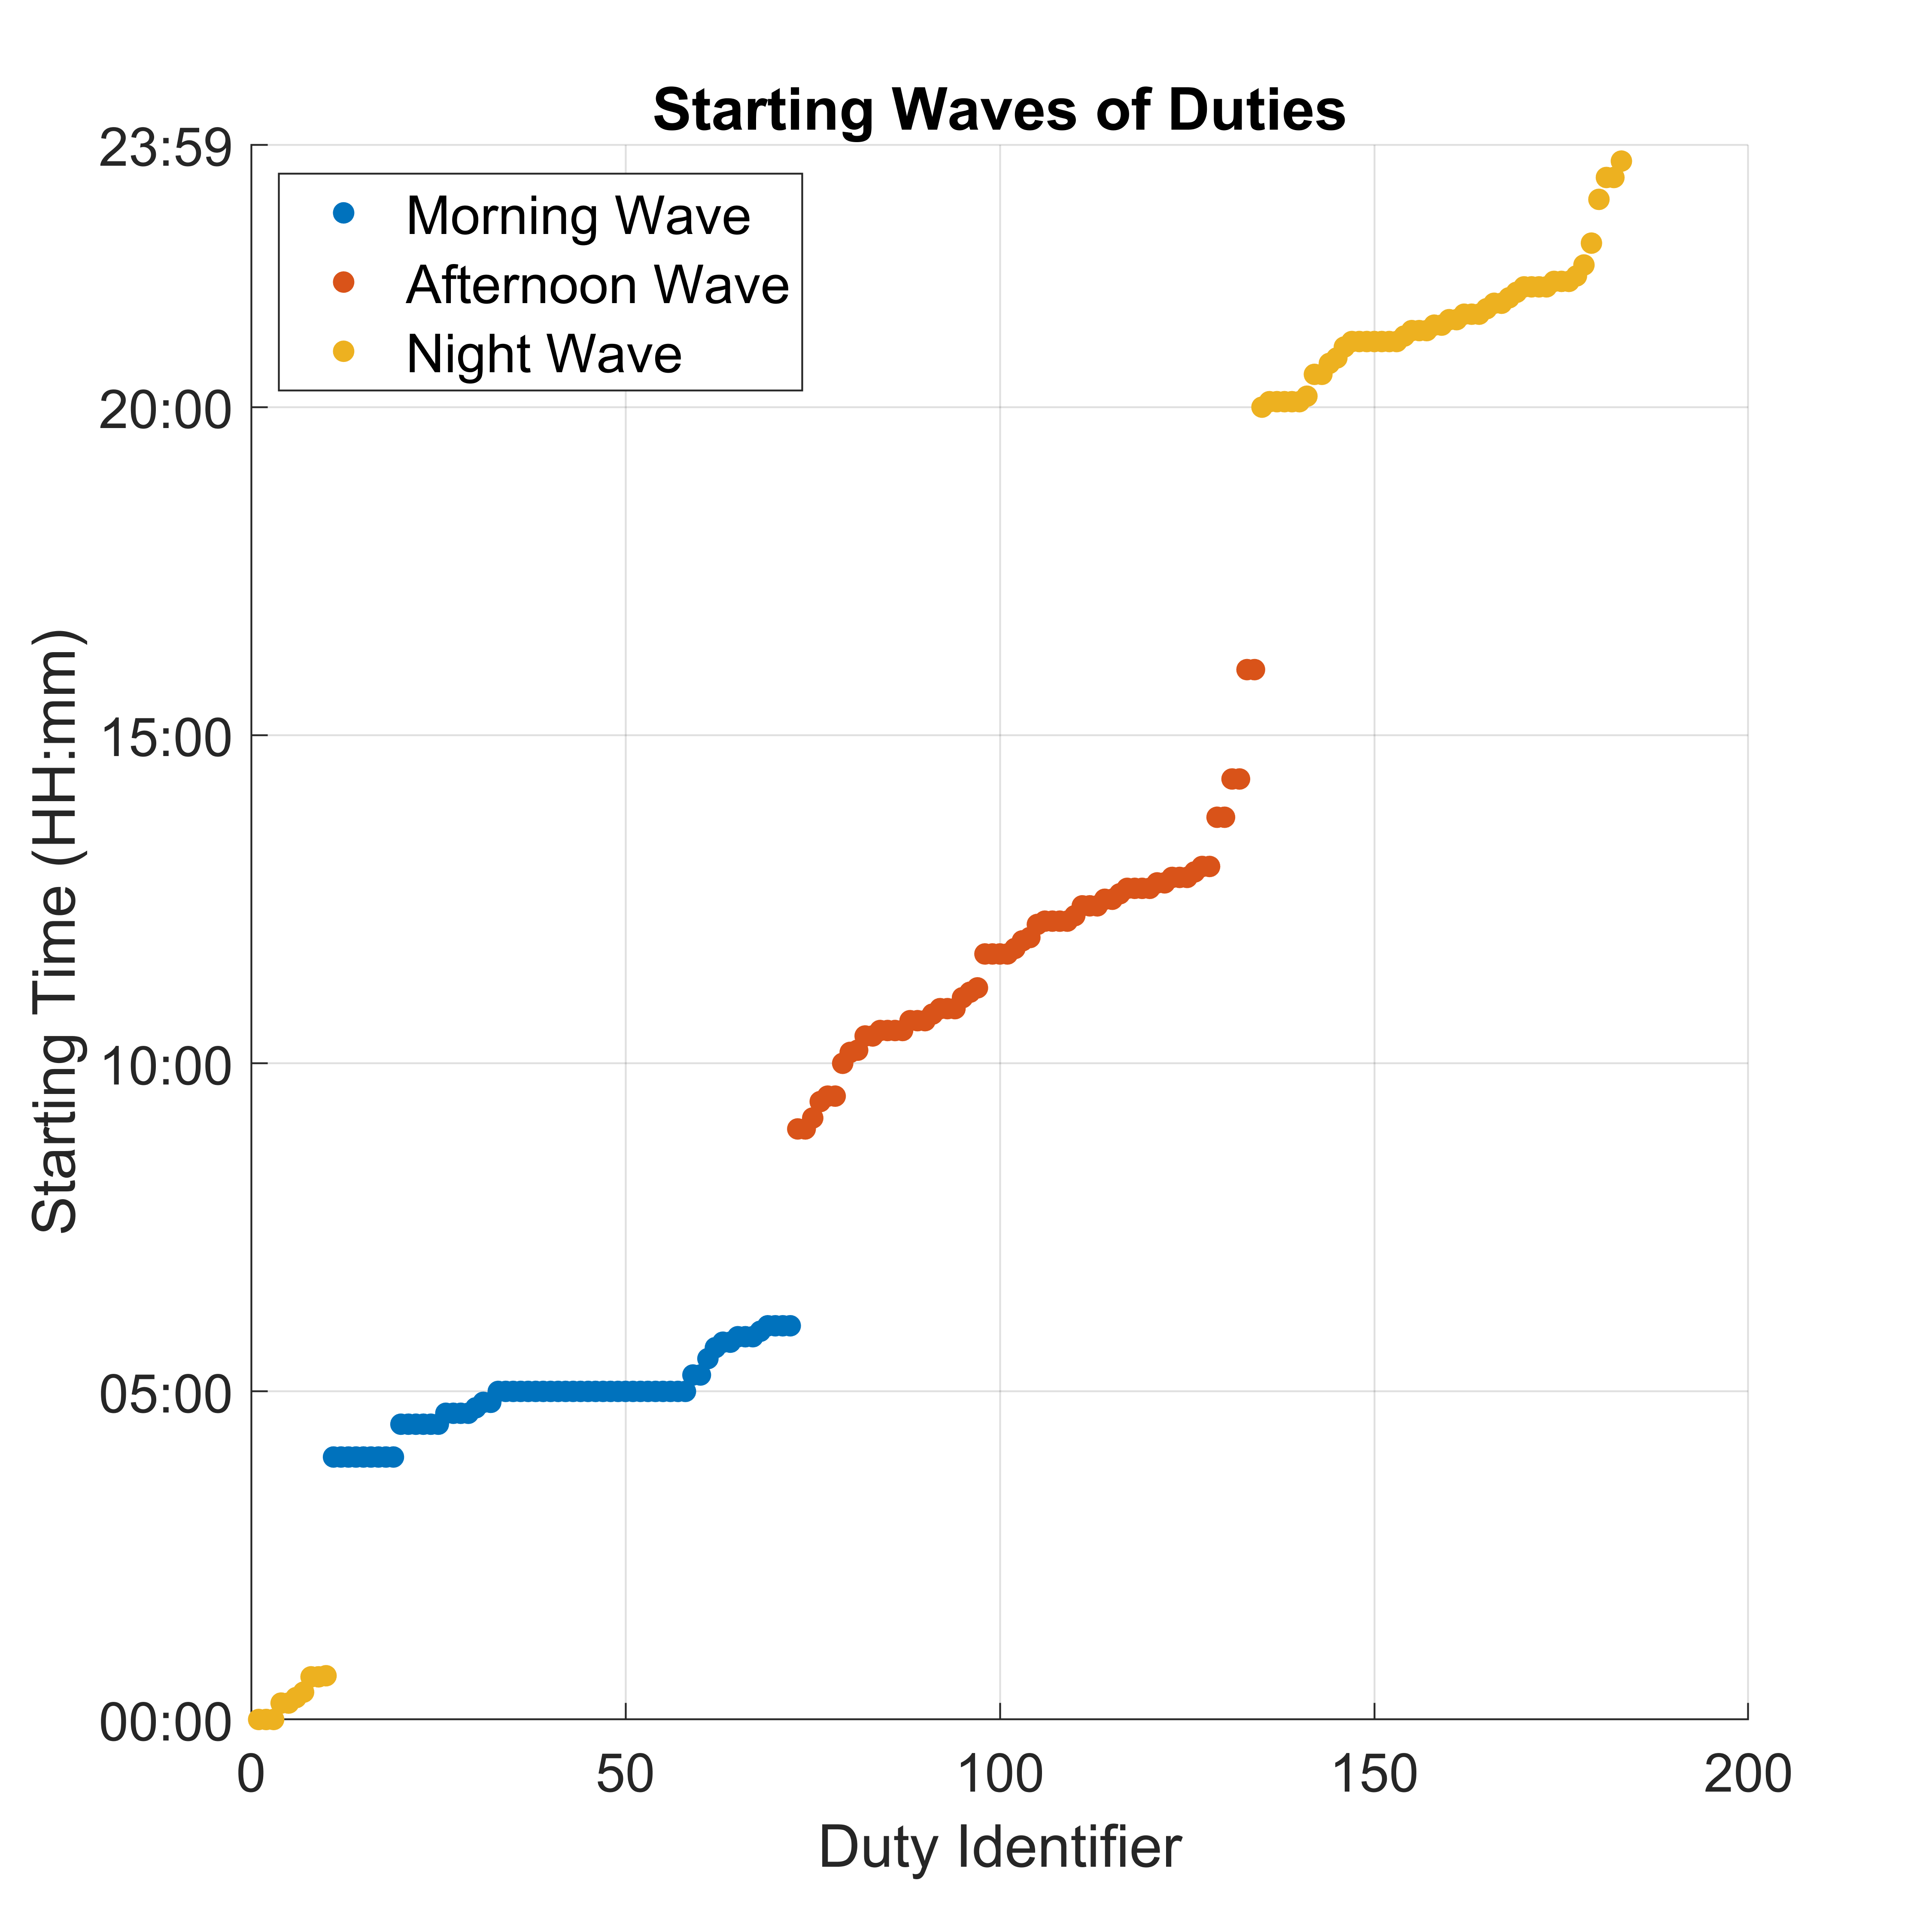
\includegraphics[width=0.46\linewidth]{appendix/Appendix-Start-wave.png}
    
\end{center}
   \caption{Plot of the starting times of duties, illustrating the wave like fashion of the starts of duties.}
\label{fig:starting time}
\end{figure}

\vspace{\baselineskip}
\noindent
Using Figure \ref{fig:starting time} as our guide, we manually characterised each cluster of starting times of duties as \textbf{wave instances}, splitting our overall dataset into the \textbf{three wave sub-instances} of Table \ref{table:Starting Waves} as outlined in Section \ref{section: Wave Instances - Data}.  

%%%%%%%%%%%%%%%%%%%%%%%%%%%%%%%%%%%%%%%%%%%%%%%%%%%%%%% Table %%%%%%%%%%%%%%%%%%%%%%%%%%%%%%%%%%%%%%%%%%%%%%%%%%%%%%%%%%%%%%%%%%%%%%%%%%%

\begin{table}[ht]
\small
    \centering 
    \begin{tabular}{|l|c|c|c|c|}
        \hline
        \textbf{Wave} & \multicolumn{4}{|c|}{ \textbf{Characteristics}} \\
        \hline
        & \textit{Start time} & \textit{End time} & \textit{Timespan}  & \textit{Number of Duties}  \\
        \hline
        \texttt{morning} & 4:00 AM & 6:00 AM & 2 hours & 60 \\
        \hline
        \texttt{afternoon} & 9:00 AM & 4:00 PM & 7 hours & 60 \\
        \hline
        \texttt{night} & 8:00 PM & 0:40 PM & 4 hours, 40 minutes & 63 \\
        \hline
    \end{tabular}%
    \medbreak
    \caption{Table outlining the Starting time, End time and Number of duties of each wave. Time values are stated in (HH:mm) AM/PM units.}
    \label{table:Starting Waves}
\end{table}

\vspace{\baselineskip}
\noindent
As we can see in Table \ref{table:Starting Waves} the waves have practically the same amount of duties, however they differ considerably in their timespan. The \texttt{morning} wave is around half the length of the \texttt{night} wave, and the \texttt{afternoon} is almost equal to the sum of the \texttt{morning, night} waves.    

%%%%%%%%%%%%%%%%%%%%%%%%%%%%%%%%%%%%%%%%%%%%%%%%%%%%%%%% sub-Section %%%%%%%%%%%%%%%%%%%%%%%%%%%%%%%%%%%%%%%%%%%%%%%%%%%%%%%%%%%%%%%%%%%%%%%%%
\subsection{Number of Daily Duties}
We thought, it would be an interesting fact to see how many duties occurred each day of the week. This information was deduced from our dataset which contained one week's worth of duties. We plotted the number of duties that occurred each day on Figure \ref{fig: Number of shifts per day}. The findings from this plot would consequently, be indicative of the number of HGV drivers required to carry out those duties per week. Hence, we can infer what Royal Mail's overall fleet of drivers looks like on a given week, since each driver performs one duty per day. 

\vspace{\baselineskip}
\noindent
We can observe from the figure that Royal Mail, requires on average around 60 drivers to be active each day of the week. Understandably considerably less drivers are required to carry out the weekend shifts since there is not much activity over the weekend.   

%%%%%%%%%%%%%%%%%%%%%%%%%%%%%%%%%%%%%%%%%%%%%%%%%%%%%%%% Figure %%%%%%%%%%%%%%%%%%%%%%%%%%%%%%%%%%%%%%%%%%%%%%%%%%%%%%%%%%%%%%%%%%%%%%%%%


\begin{figure}[ht]
\begin{center}
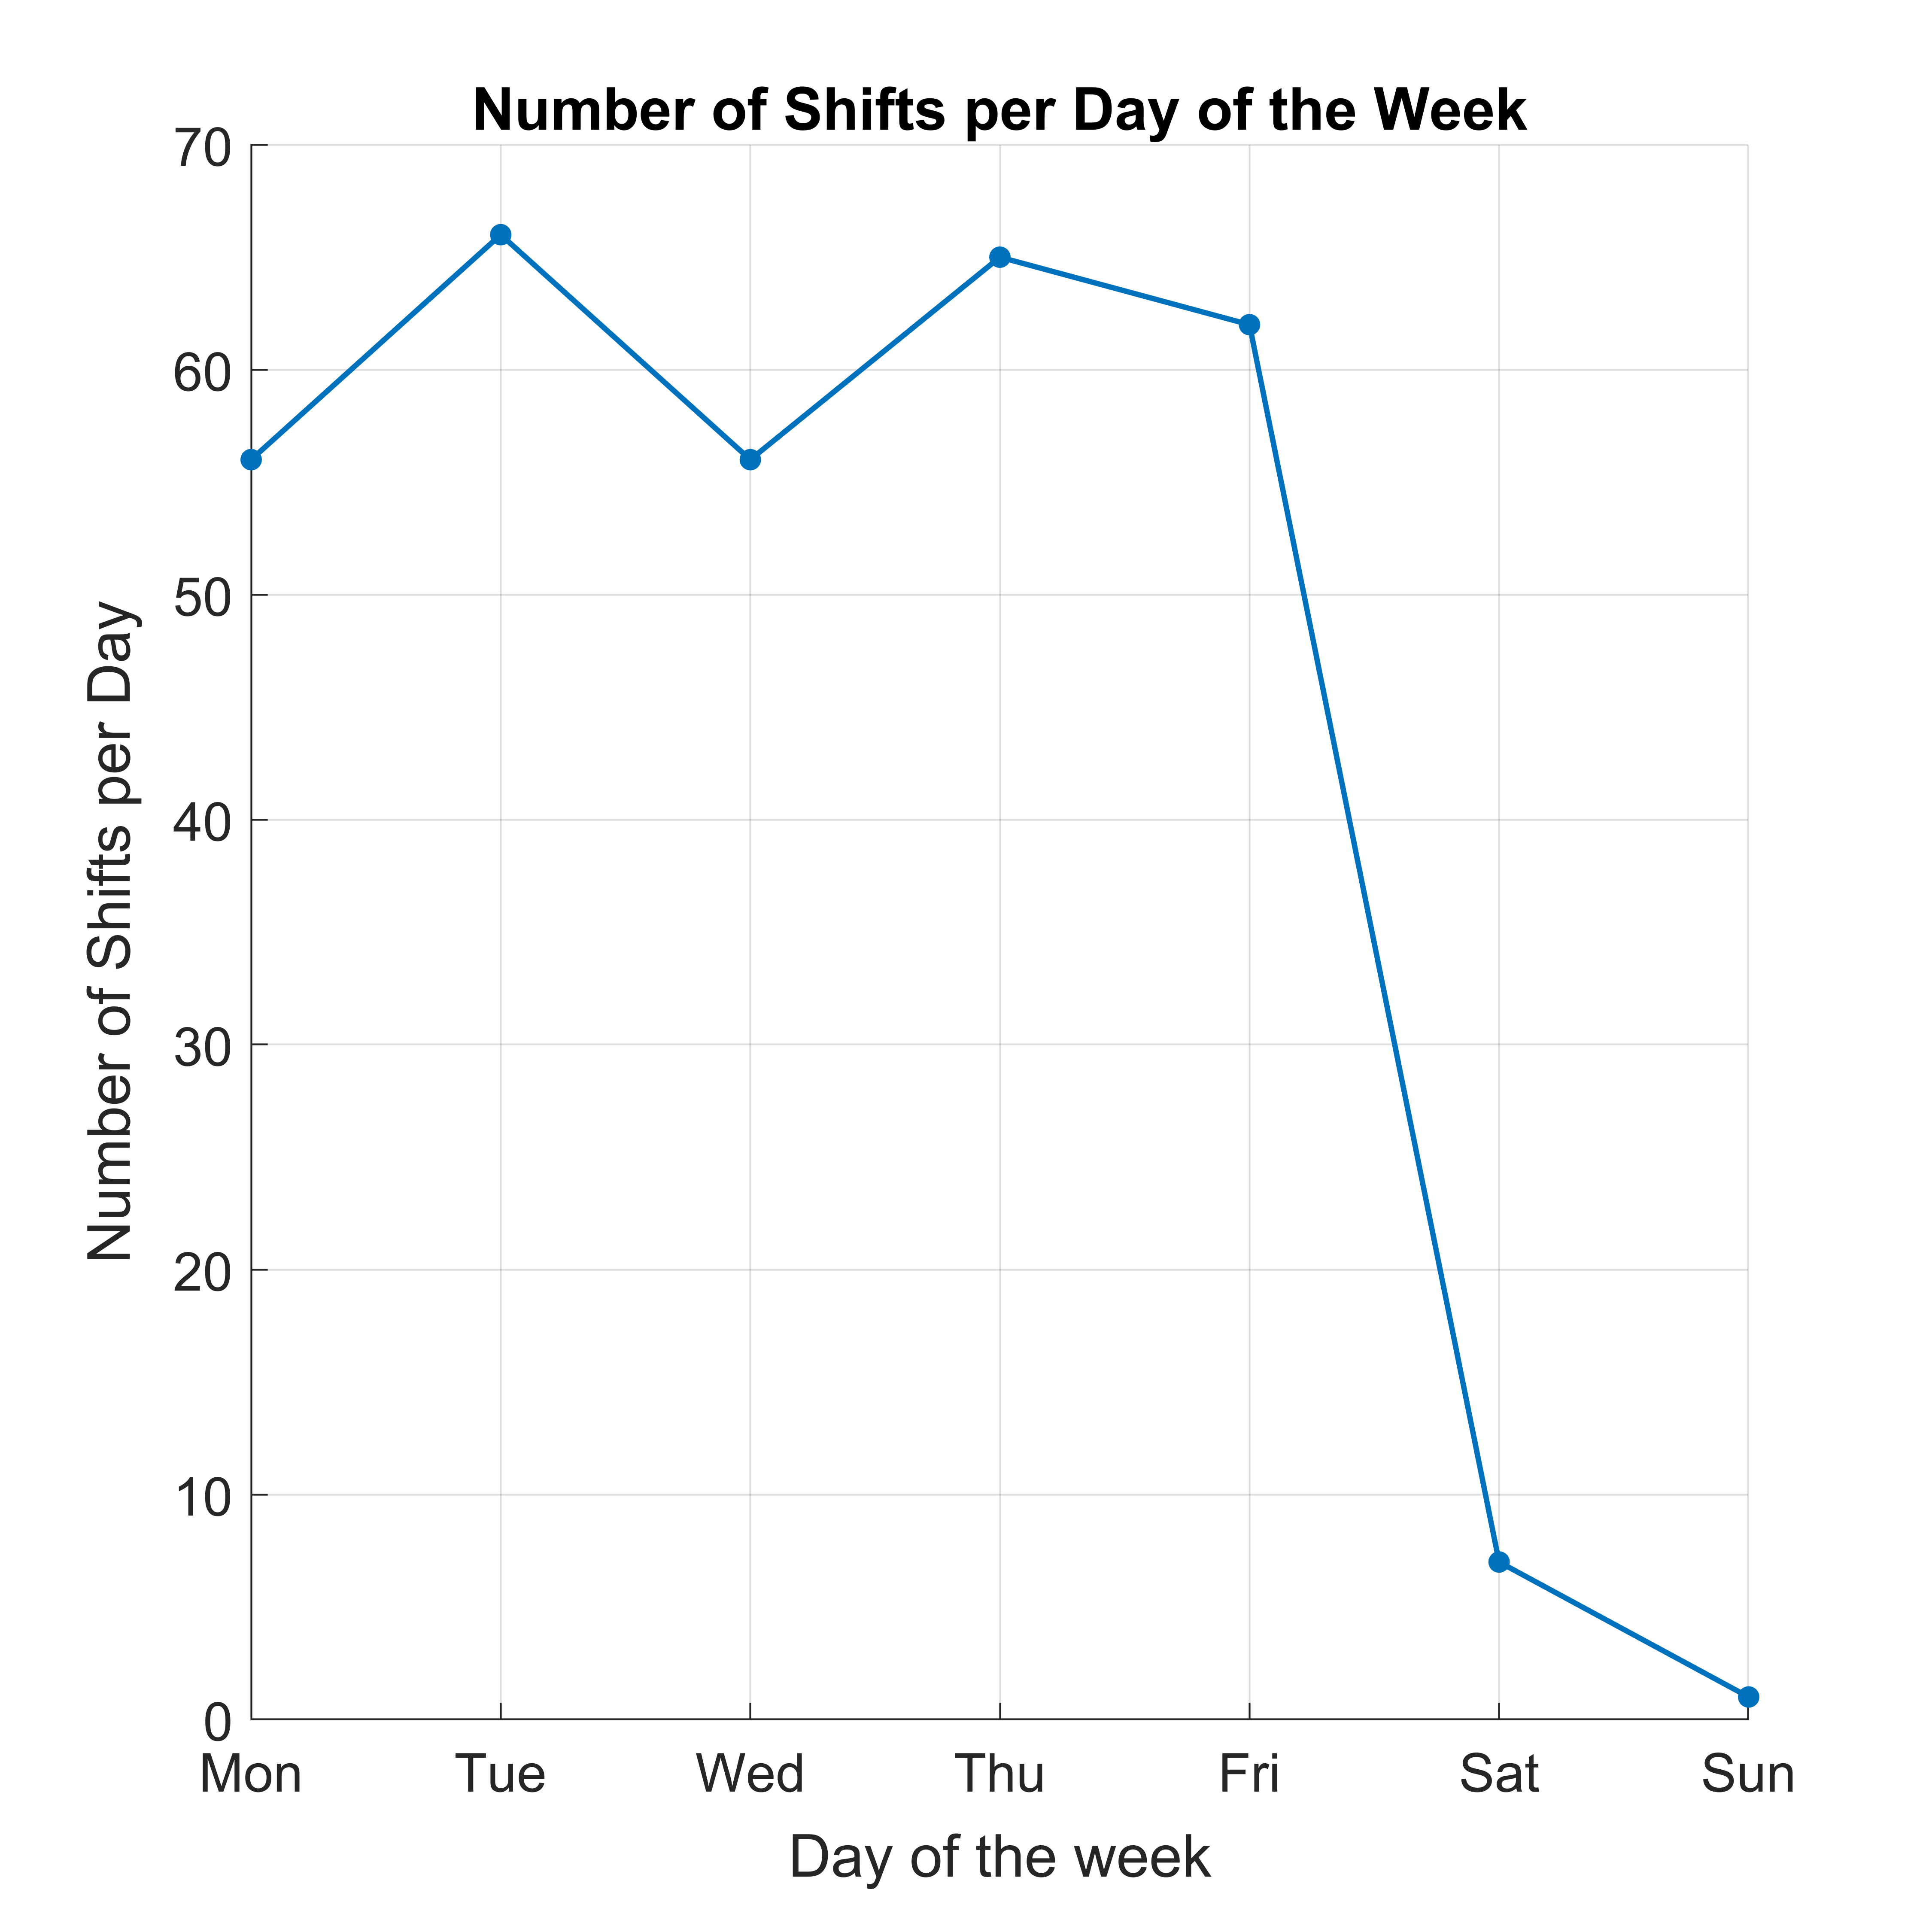
\includegraphics[width=0.46\linewidth]{appendix/shift per day.png}
    
\end{center}
   \caption{Plot of the number of shifts occurring each day.}
\label{fig: Number of shifts per day}
\end{figure}

%%%%%%%%%%%%%%%%%%%%%%%%%%%%%%%%%%%%%%%%%%%%%%%%%%%%%%%% Section %%%%%%%%%%%%%%%%%%%%%%%%%%%%%%%%%%%%%%%%%%%%%%%%%%%%%%%%%%%%%%%%%%%%%%%%%

\section{Operations on Historical Schedules}

%%%%%%%%%%%%%%%%%%%%%%%%%%%%%%%%%%%%%%%%%%%%%%%%%%%%%%%% Sub-Section %%%%%%%%%%%%%%%%%%%%%%%%%%%%%%%%%%%%%%%%%%%%%%%%%%%%%%%%%%%%%%%%%%%%%%%%%
\subsection{Redefining Historical Schedules}
\label{subsection: redefine appexnix}
%%%%%%%%%%%%%%%%%%%%%%%%%%%%%%%%%%%%%%%%%%%%%%%%%%%%%%%%%%%%%%%%%%%%%%%%%%%%%%% Figure %%%%%%%%%%%%%%%%%%%%%%%%%%%%%%%%%%%%%%%%%%%%%%%%%%%%%%%%%%%%%%%%%%%%%%%%%%%%%%

\begin{figure}[ht]
    \centering
    \subfloat[\textit{Duty lengths} sorted in increasing order, showing the effect of deleting the \textbf{non-useful} activities.]{%\begin{center}
    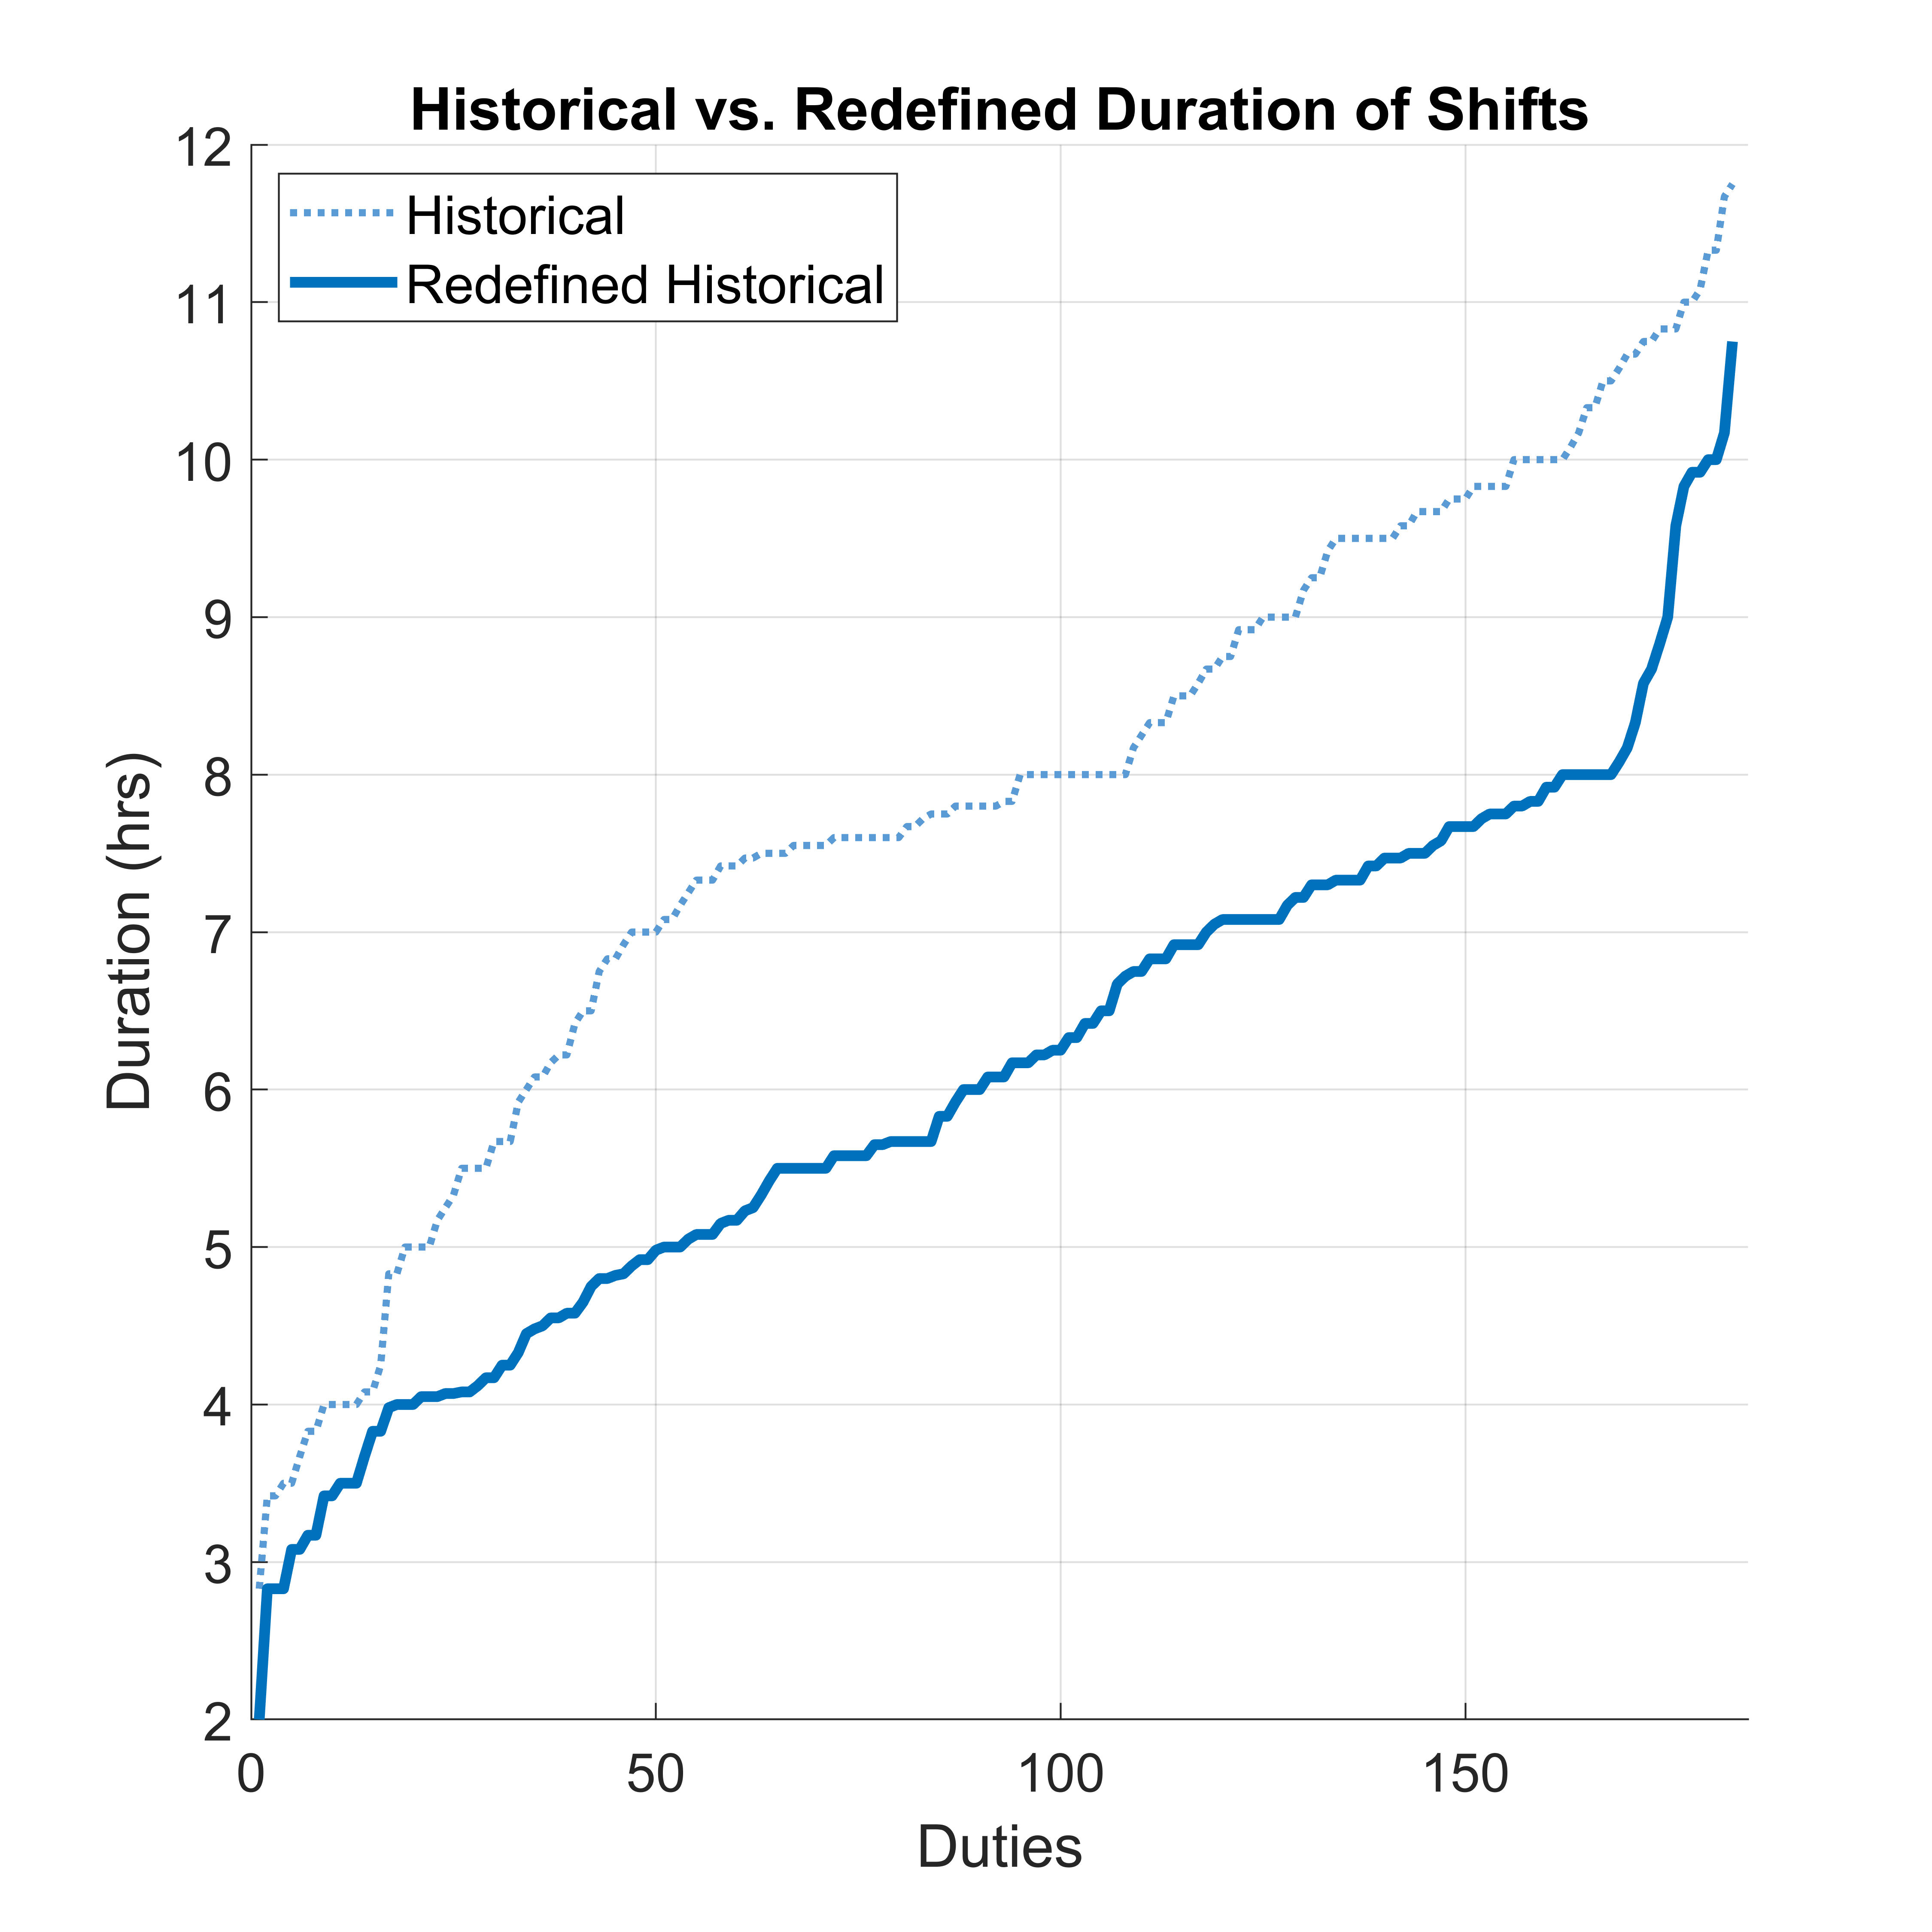
\includegraphics[width=0.46\linewidth]{[1] - chapter/Image Files/1-Effect-of-Redefined.png}
    }%\end{center}}%picture #1
    \qquad
    %picture #2
    \centering
    \subfloat[Histogram showing the effect of Redefining the dataset.]{%\begin{center}
    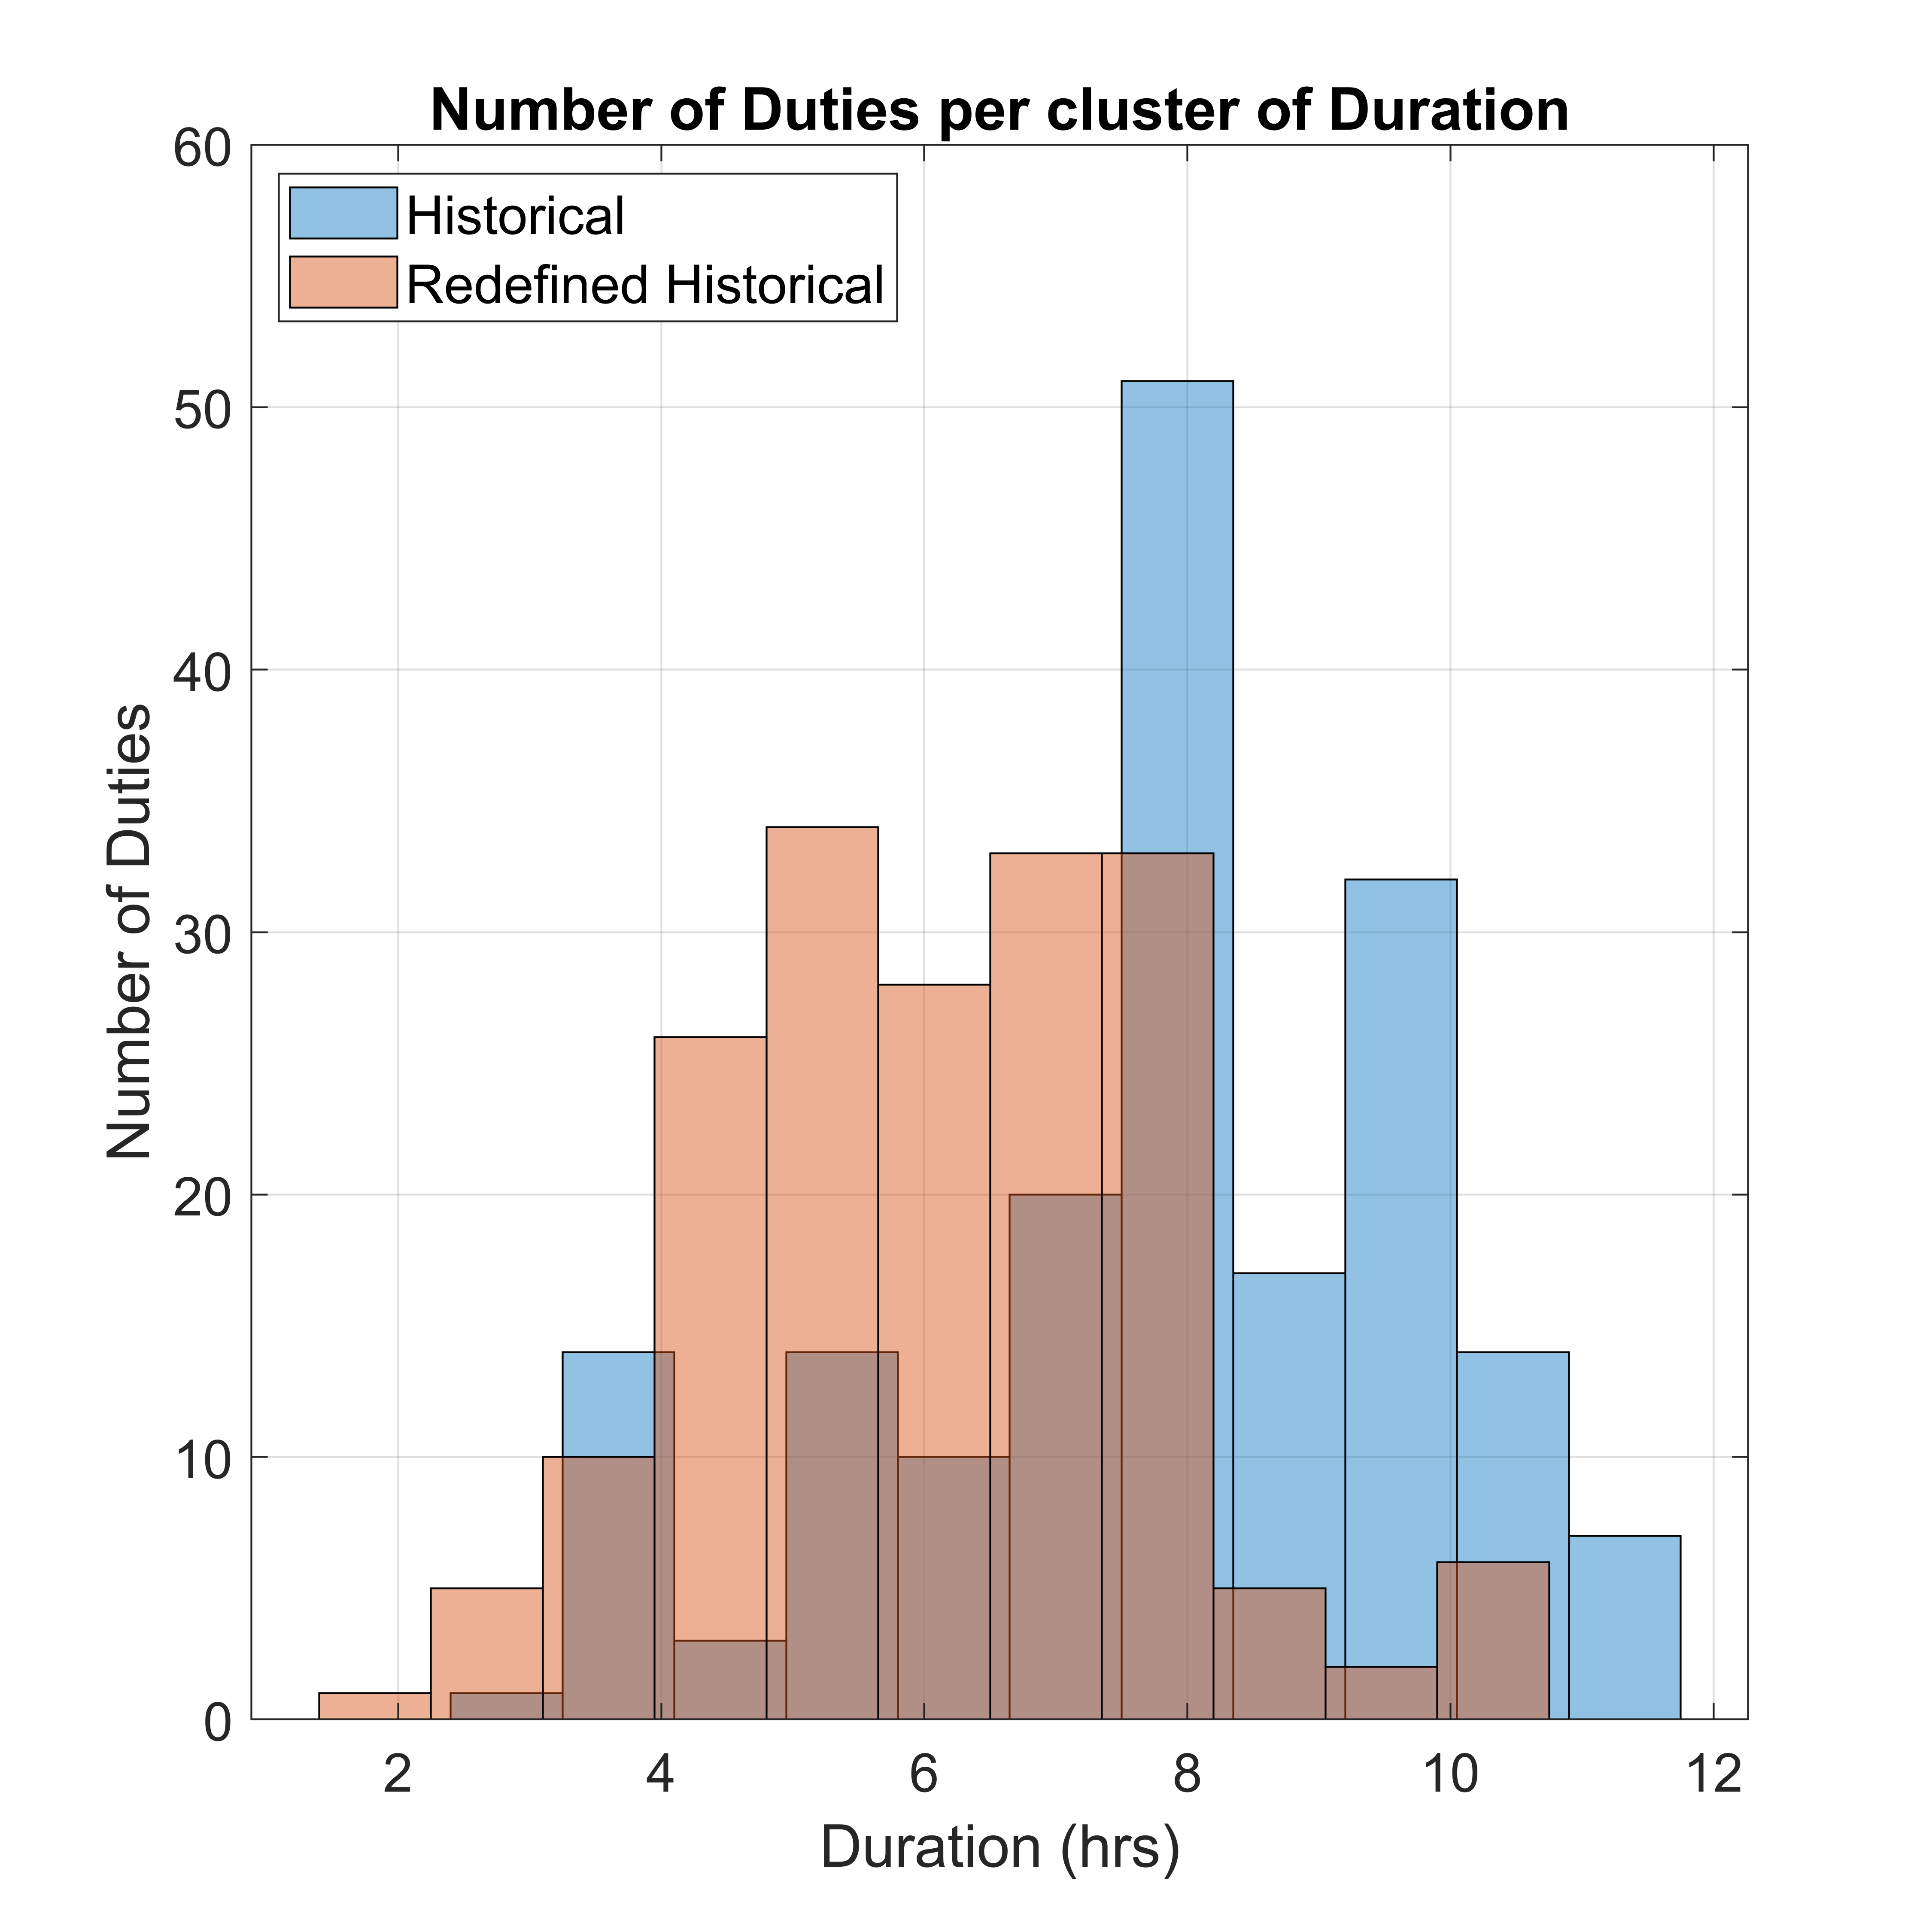
\includegraphics[width=0.46\linewidth]{[1] - chapter/Image Files/1-Effect-of-Redefined-histogram.png}
    }%\end{center}}%end of picture #2
    \caption{Figures illustrating the effects of the Redefining the dataset by deleting the \textbf{non-useful} activities from the Historical Schedule.}%
    \label{fig: Redefined Historical.}%
\end{figure}

In this section we discuss the effects of the operation carried out in Section \ref{section: Redefined Dataset} regarding the deletion of \textbf{non-useful} activities from the original dataset. As one can see Figure \ref{fig: Redefined Historical.}(a) there is a step change deletion of overall time to be schedule from the Historical dataset, once we delete the non-useful activities. Subsequently, Figure \ref{fig: Redefined Historical.}(b) shows the same effect as observed in a histogram graph. The deletion of the non-useful time is observed as a horizontal shift to of the histogram to the left, signifying the fact that less overall hours are not contained in the schedule.

\vspace{\baselineskip}
\noindent
The operation of deleting the activities has a direct impact on the structure of the blocks. Namely, blocks that contain such \textbf{non-useful} activities will see their duration decreased. This is seen more practically in the following table:

%%%%%%%%%%%%%%%%%%%%%%%%%%%%%%%%%%%%%%%%%%%%%%%%%%%%%%%%%%%%%%%%%%%%%% Table %%%%%%%%%%%%%%%%%%%%%%%%%%%%%%%%%%%%%%%%%%%%%%%

\begin{table}[ht]
\small
    \centering 
    \begin{tabular}{|c|c|c|c|}
        \hline
        \textbf{Instance} & \multicolumn{3}{|c|}{ \textbf{Blocks (HH:mm)}}  \\
        \hline
         & \texttt{Average} &  \texttt{Minimum} & \texttt{Maximum} \\
        \hline
        Historical & 03:05 & 00:40 & 08:25 \\
        \hline
        Morning & 03:28 & 00:50 & 08:25 \\
        \hline
        Afternoon & 03:05 & 01:10 & 07:20 \\
        \hline
        Night & 02:52 & 00:40 & 07:30 \\
        \hline
    \end{tabular}%
    \medbreak
\end{table}

%%%%%%%%%%%%%%%%%%%%%%%%%%%%%%%%%%%%%%%%%%%%%%%%%%%%%%%% Sub-Section %%%%%%%%%%%%%%%%%%%%%%%%%%%%%%%%%%%%%%%%%%%%%%%%%%%%%%%%%%%%%%%%%%%%%%%%%

\subsection{Comparison of Disturbed Nominal and Optimised Schedules}
\label{subsection: Appendix Comparison of Disturbed Nominal and Optimised Schedules}
In Figure \ref{fig: Nominal Uncertainty Sets Effects.} our goal is to determine the robustness to uncertainty of the nominal schedule. To identify its level of robustness we compare, for of the three uncertainty sets, the disturbed instance optimised under uncertainty with the nominal schedule disturbed with the same instance. There are two such cases for each uncertainty set, one that involves instances that have been \texttt{reduced}, with respect to the overall time scheduled, after the application of uncertainty, and those that have been \texttt{augmented} respectively. The former are presented in Figure \ref{fig: Nominal Uncertainty Sets Effects.}(a) while the latter in Figure \ref{fig: Nominal Uncertainty Sets Effects.}(b). 

%%%%%%%%%%%%%%%%%%%%%%%%%%%%%%%%%%%%%%%%%%%%%%%%%%%%%%% Double Figure %%%%%%%%%%%%%%%%%%%%%%%%%%%%%%%%%%%%%%%%%%%%%%%%%%%%%%%%%%%%%%%%%%%%%%%%%%%

\begin{figure}[ht]
    \centering
    \subfloat[Disturbed instances with a \textbf{decrease} in overall labor time (\texttt{reduced}).]{%\begin{center}
    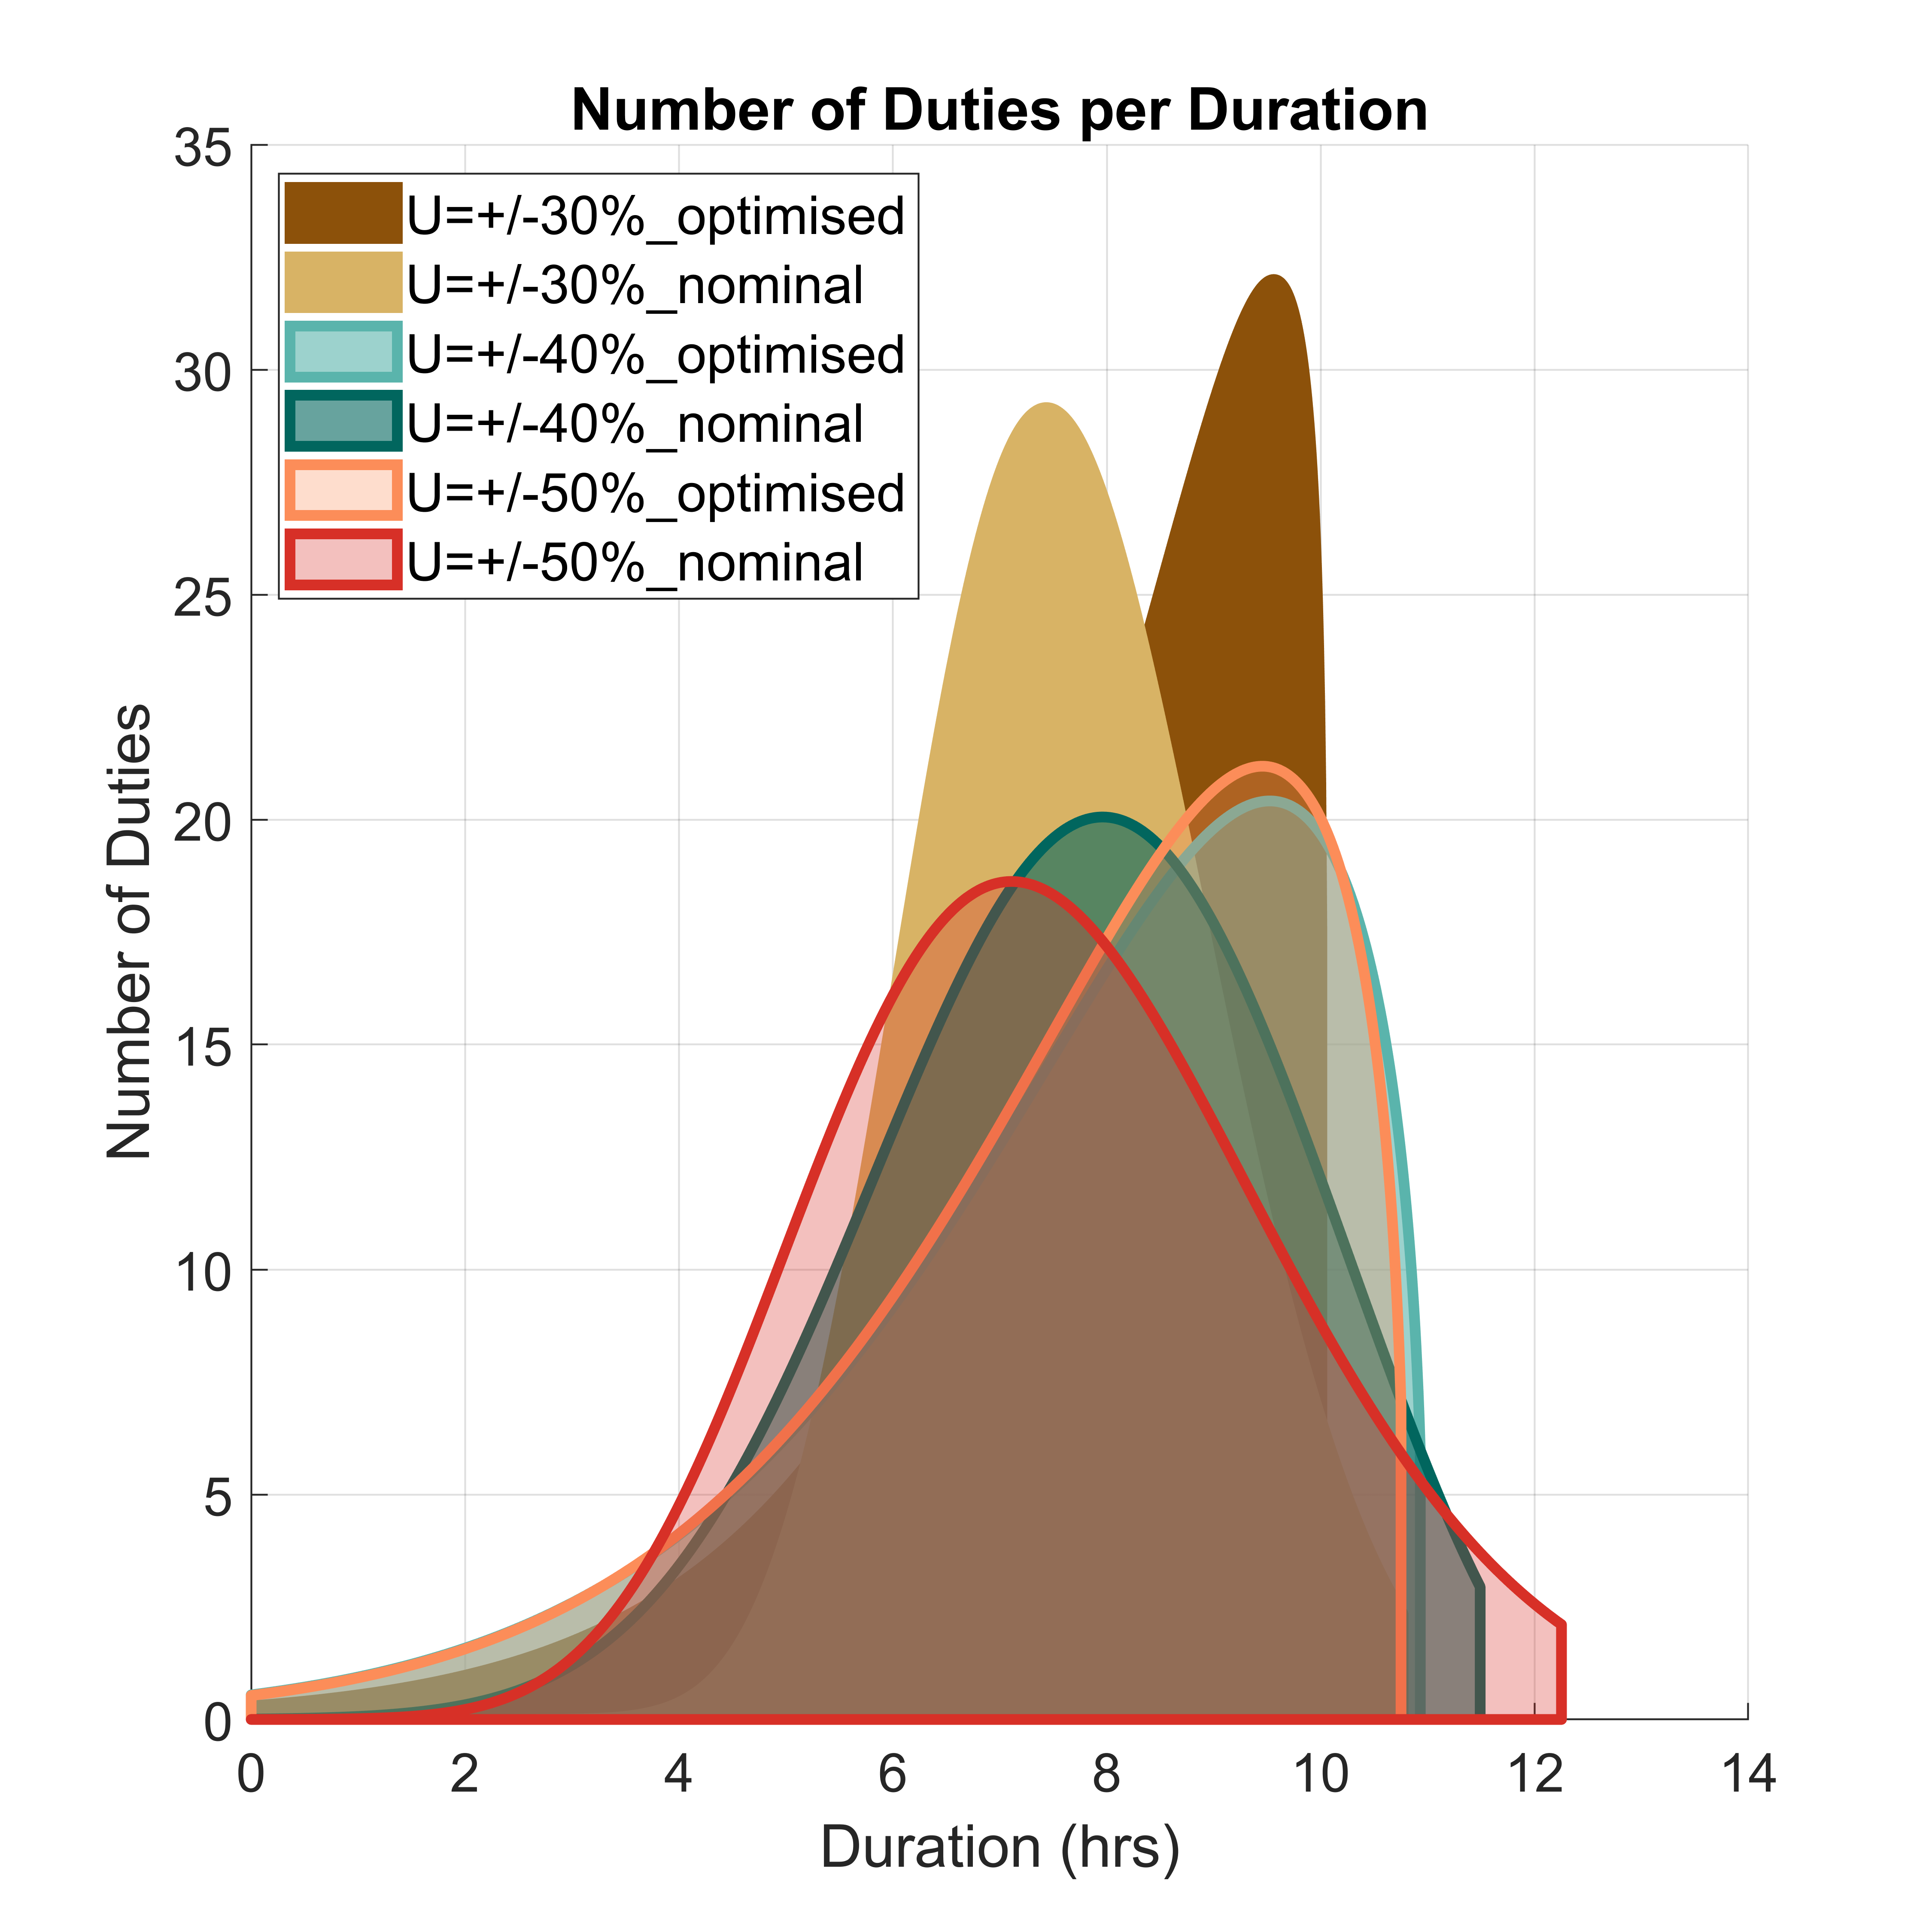
\includegraphics[width=0.46\linewidth]{appendix/Comparison_Of_Uncertainty_Sets_min_and_nominal.png}
    }%\end{center}}%end of picture #2
    \qquad
    %picture #2
    \centering
    \subfloat[Disturbed instances with an \textbf{increase} in overall labor time (\texttt{augmented}).]{%\begin{center}
    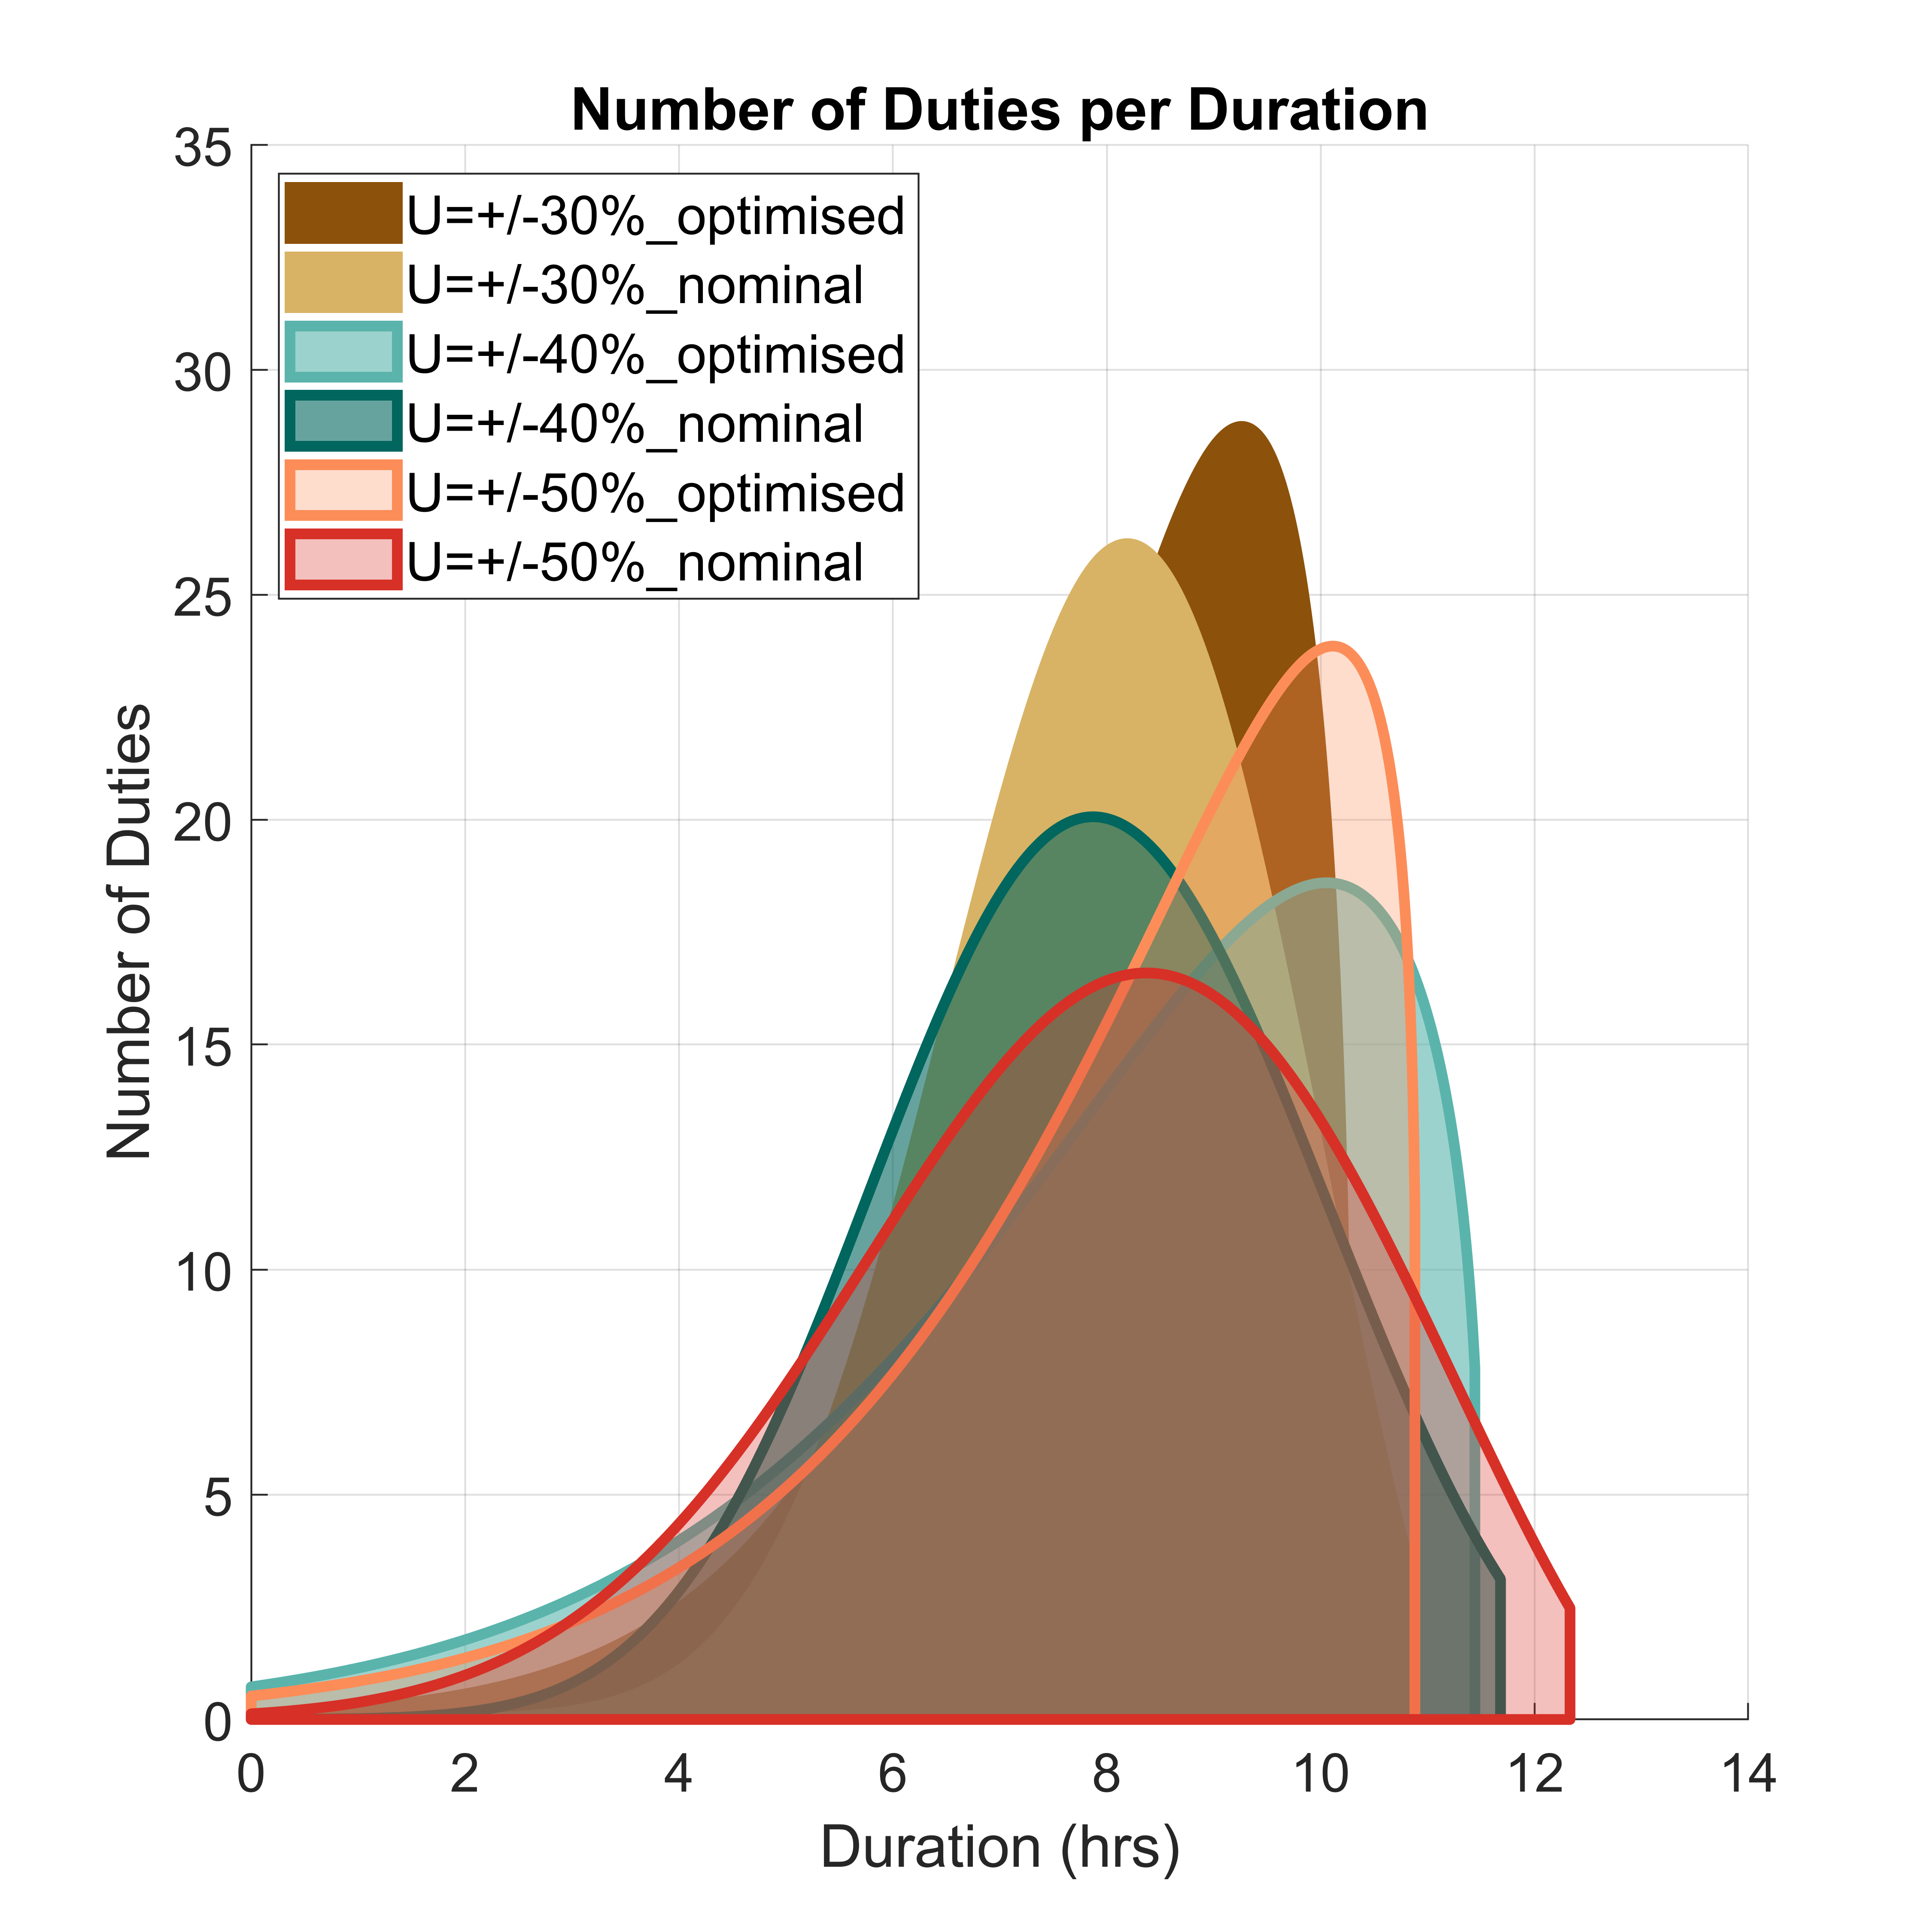
\includegraphics[width=0.46\linewidth]{appendix/Comparison_Of_Uncertainty_Sets_max_and_nominal.png}
    }%\end{center}}%picture #1
    \caption{The histograms provide an overview of the effects of various levels of uncertainty set on $Duty$ lengths.}
    \label{fig: Nominal Uncertainty Sets Effects.}
\end{figure}
 



%%%%%%%%%%%%%%%%%%%%%%%%%%%%%%%%%%%%%%%%%%%%%%%%%%%%%%%% Section %%%%%%%%%%%%%%%%%%%%%%%%%%%%%%%%%%%%%%%%%%%%%%%%%%%%%%%%%%%%%%%%%%%%%%%%%
\section{Supporting Notes}

%%%%%%%%%%%%%%%%%%%%%%%%%%%%%%%%%%%%%%%%%%%%%%%%%%%%%%%% Sub-Section %%%%%%%%%%%%%%%%%%%%%%%%%%%%%%%%%%%%%%%%%%%%%%%%%%%%%%%%%%%%%%%%%%%%%%%%%

\subsection{EU Directives for HGV Drivers}
\label{section: EU rules}
This section makes reference to the  European Union (EU) rules on drivers' hours and working time as dictated by the Department for Transport (DfT). This is an important real-life aspect of our problem, that is mentioned and referred to, at various points in the report. %link: https://assets.publishing.service.gov.uk/government/uploads/system/uploads/attachment_data/file/856360/simplified-guidance-eu-drivers-hours-working-time-rules.pdf

\begin{enumerate}[label=\textbf{(\arabic*)}]
    \item \textbf{\underline{Driving-time Directive}: }
       
       \vspace{\baselineskip}
        \noindent
        \begin{enumerate}[label=\roman*]
       \item \underline{Time Limit:}
       
        \begin{itemize}
            \item 9 hours daily driving limit.
            \item Maximum of 56 hours weekly driving limit.      
            \item Maximum of 90 hours fortnightly driving limit.
        \end{itemize} 
        
        \vspace{\baselineskip}
        \noindent
      \item  \underline{Break:}
        \begin{itemize}
        \item 45 minutes break after 4.5 hours driving
        \end{itemize} 
        \end{enumerate}

    \item \textbf{\underline{Working-time Directive}: }
    
      \vspace{\baselineskip}
      \noindent
      \begin{enumerate}[label=\roman*]
    \item  \underline{Time Limit:}
    
        \begin{itemize}
            \item Working time must not exceed average of 48 hours a week.
            \item Maximum working time of 60 hours in one week.
            \item Maximum working time of 10 hours if night work performed.
        \end{itemize}  
        
        
        \vspace{\baselineskip}
        \noindent
    \item    \underline{Break:}
        \begin{itemize}
        \item Cannot work for more than 6 hours without a break. A break should be at least 15 minutes long
        \item 30 minute break if working between 6 and 9 hours in total
        \item 45 minute break if working more than 9 hours in total
        \end{itemize} 
        \end{enumerate}

\end{enumerate}

        
%%%%%%%%%%%%%%%%%%%%%%%%%%%%%%%%%%%%%%%%%%%%%%%%%%%%%%%% Sub-Section %%%%%%%%%%%%%%%%%%%%%%%%%%%%%%%%%%%%%%%%%%%%%%%%%%%%%%%%%%%%%%%%%%%%%%%%%        
\subsection{Relaxation of a Mathematical Program}
\label{section: Appednix Relaxation}
In order to utilise the efficacy of the simplex algorithm, and apply to solve MILPs we require to obtain the relaxation of an integer-linear program into a LP. A relaxed version of an integer program is defined as below.

\begin{equation}
\begin{aligned}
& \underset{x}{\text{minimise}}
& & f(x) \\
& \text{subject to}
& & h_i(x) = 0 \\
& & & g_j(x) \leq 0 \\
\end{aligned}
\end{equation}
\[\text{where} \; x \in S_{original}\]

\noindent
with the corresponding \textbf{relaxed} version of the problem,\par

\begin{equation}
\begin{aligned}
& \underset{x}{\text{minimise}}
& & f(x) \\
& \text{subject to}
& & h_i(x) = 0 \\
& & & g_j(x) \leq 0 \\
\end{aligned}
\end{equation}
\[\text{where} \; x \in S_{relaxed} \; \text{and} \; S_{original} \subseteq S_{relaxed}\]

\vspace{\baselineskip}
\noindent
The relaxation of a problem is usually obtained by the removal of one or more constraints of the original formulation. For example, when obtaining the relaxation of an integer program, we usually refer to the process of neglecting the integrality constraint on the integer program's decision variable(s) to transform our problem into a standard LP.






\bibliographystyle{vancouver}
\bibliography{bibs/sample}

\end{document}